% Options for packages loaded elsewhere
\PassOptionsToPackage{unicode}{hyperref}
\PassOptionsToPackage{hyphens}{url}
%
\documentclass[
]{book}
\usepackage{lmodern}
\usepackage{amssymb,amsmath}
\usepackage{ifxetex,ifluatex}
\ifnum 0\ifxetex 1\fi\ifluatex 1\fi=0 % if pdftex
  \usepackage[T1]{fontenc}
  \usepackage[utf8]{inputenc}
  \usepackage{textcomp} % provide euro and other symbols
\else % if luatex or xetex
  \usepackage{unicode-math}
  \defaultfontfeatures{Scale=MatchLowercase}
  \defaultfontfeatures[\rmfamily]{Ligatures=TeX,Scale=1}
\fi
% Use upquote if available, for straight quotes in verbatim environments
\IfFileExists{upquote.sty}{\usepackage{upquote}}{}
\IfFileExists{microtype.sty}{% use microtype if available
  \usepackage[]{microtype}
  \UseMicrotypeSet[protrusion]{basicmath} % disable protrusion for tt fonts
}{}
\makeatletter
\@ifundefined{KOMAClassName}{% if non-KOMA class
  \IfFileExists{parskip.sty}{%
    \usepackage{parskip}
  }{% else
    \setlength{\parindent}{0pt}
    \setlength{\parskip}{6pt plus 2pt minus 1pt}}
}{% if KOMA class
  \KOMAoptions{parskip=half}}
\makeatother
\usepackage{xcolor}
\IfFileExists{xurl.sty}{\usepackage{xurl}}{} % add URL line breaks if available
\IfFileExists{bookmark.sty}{\usepackage{bookmark}}{\usepackage{hyperref}}
\hypersetup{
  pdftitle={The Worst Stats Text eveR},
  pdfauthor={Dan Stich},
  hidelinks,
  pdfcreator={LaTeX via pandoc}}
\urlstyle{same} % disable monospaced font for URLs
\usepackage{color}
\usepackage{fancyvrb}
\newcommand{\VerbBar}{|}
\newcommand{\VERB}{\Verb[commandchars=\\\{\}]}
\DefineVerbatimEnvironment{Highlighting}{Verbatim}{commandchars=\\\{\}}
% Add ',fontsize=\small' for more characters per line
\usepackage{framed}
\definecolor{shadecolor}{RGB}{248,248,248}
\newenvironment{Shaded}{\begin{snugshade}}{\end{snugshade}}
\newcommand{\AlertTok}[1]{\textcolor[rgb]{0.94,0.16,0.16}{#1}}
\newcommand{\AnnotationTok}[1]{\textcolor[rgb]{0.56,0.35,0.01}{\textbf{\textit{#1}}}}
\newcommand{\AttributeTok}[1]{\textcolor[rgb]{0.77,0.63,0.00}{#1}}
\newcommand{\BaseNTok}[1]{\textcolor[rgb]{0.00,0.00,0.81}{#1}}
\newcommand{\BuiltInTok}[1]{#1}
\newcommand{\CharTok}[1]{\textcolor[rgb]{0.31,0.60,0.02}{#1}}
\newcommand{\CommentTok}[1]{\textcolor[rgb]{0.56,0.35,0.01}{\textit{#1}}}
\newcommand{\CommentVarTok}[1]{\textcolor[rgb]{0.56,0.35,0.01}{\textbf{\textit{#1}}}}
\newcommand{\ConstantTok}[1]{\textcolor[rgb]{0.00,0.00,0.00}{#1}}
\newcommand{\ControlFlowTok}[1]{\textcolor[rgb]{0.13,0.29,0.53}{\textbf{#1}}}
\newcommand{\DataTypeTok}[1]{\textcolor[rgb]{0.13,0.29,0.53}{#1}}
\newcommand{\DecValTok}[1]{\textcolor[rgb]{0.00,0.00,0.81}{#1}}
\newcommand{\DocumentationTok}[1]{\textcolor[rgb]{0.56,0.35,0.01}{\textbf{\textit{#1}}}}
\newcommand{\ErrorTok}[1]{\textcolor[rgb]{0.64,0.00,0.00}{\textbf{#1}}}
\newcommand{\ExtensionTok}[1]{#1}
\newcommand{\FloatTok}[1]{\textcolor[rgb]{0.00,0.00,0.81}{#1}}
\newcommand{\FunctionTok}[1]{\textcolor[rgb]{0.00,0.00,0.00}{#1}}
\newcommand{\ImportTok}[1]{#1}
\newcommand{\InformationTok}[1]{\textcolor[rgb]{0.56,0.35,0.01}{\textbf{\textit{#1}}}}
\newcommand{\KeywordTok}[1]{\textcolor[rgb]{0.13,0.29,0.53}{\textbf{#1}}}
\newcommand{\NormalTok}[1]{#1}
\newcommand{\OperatorTok}[1]{\textcolor[rgb]{0.81,0.36,0.00}{\textbf{#1}}}
\newcommand{\OtherTok}[1]{\textcolor[rgb]{0.56,0.35,0.01}{#1}}
\newcommand{\PreprocessorTok}[1]{\textcolor[rgb]{0.56,0.35,0.01}{\textit{#1}}}
\newcommand{\RegionMarkerTok}[1]{#1}
\newcommand{\SpecialCharTok}[1]{\textcolor[rgb]{0.00,0.00,0.00}{#1}}
\newcommand{\SpecialStringTok}[1]{\textcolor[rgb]{0.31,0.60,0.02}{#1}}
\newcommand{\StringTok}[1]{\textcolor[rgb]{0.31,0.60,0.02}{#1}}
\newcommand{\VariableTok}[1]{\textcolor[rgb]{0.00,0.00,0.00}{#1}}
\newcommand{\VerbatimStringTok}[1]{\textcolor[rgb]{0.31,0.60,0.02}{#1}}
\newcommand{\WarningTok}[1]{\textcolor[rgb]{0.56,0.35,0.01}{\textbf{\textit{#1}}}}
\usepackage{longtable,booktabs}
% Correct order of tables after \paragraph or \subparagraph
\usepackage{etoolbox}
\makeatletter
\patchcmd\longtable{\par}{\if@noskipsec\mbox{}\fi\par}{}{}
\makeatother
% Allow footnotes in longtable head/foot
\IfFileExists{footnotehyper.sty}{\usepackage{footnotehyper}}{\usepackage{footnote}}
\makesavenoteenv{longtable}
\usepackage{graphicx,grffile}
\makeatletter
\def\maxwidth{\ifdim\Gin@nat@width>\linewidth\linewidth\else\Gin@nat@width\fi}
\def\maxheight{\ifdim\Gin@nat@height>\textheight\textheight\else\Gin@nat@height\fi}
\makeatother
% Scale images if necessary, so that they will not overflow the page
% margins by default, and it is still possible to overwrite the defaults
% using explicit options in \includegraphics[width, height, ...]{}
\setkeys{Gin}{width=\maxwidth,height=\maxheight,keepaspectratio}
% Set default figure placement to htbp
\makeatletter
\def\fps@figure{htbp}
\makeatother
\setlength{\emergencystretch}{3em} % prevent overfull lines
\providecommand{\tightlist}{%
  \setlength{\itemsep}{0pt}\setlength{\parskip}{0pt}}
\setcounter{secnumdepth}{5}
\usepackage{booktabs}
\usepackage[]{natbib}
\bibliographystyle{apalike}

\title{The Worst Stats Text eveR}
\author{Dan Stich}
\date{}

\begin{document}
\maketitle

{
\setcounter{tocdepth}{1}
\tableofcontents
}
\hypertarget{title}{%
\chapter*{The Worst Stats Text eveR}\label{title}}
\addcontentsline{toc}{chapter}{The Worst Stats Text eveR}

Dan Stich, PhD

\emph{Biology Department and Biological Field Station, SUNY Oneonta}

Unskillful representation of an alcohol molecule where -OH is the functional group and R is the radical group, or ``rest of the molecule'', much like it is to modern statistics. This is funny, because R is a ``functional'' programming language that will drive you to drink (or perhaps undertake some other, healthier stress-reducing activity). Don't worry, I'll explain all of the jokes, and \textbf{most} of the code as we go, because this

is \textbf{The Worst Stats Text eveR}.

\hypertarget{preface}{%
\chapter*{Preface}\label{preface}}
\addcontentsline{toc}{chapter}{Preface}

\begin{center}\rule{0.5\linewidth}{0.5pt}\end{center}

This book is a compilation of teaching content and lab activities that I have amassed like a digital hoarder during my time teaching BIOL 217 (Quantitative Biology) at SUNY Oneonta. The book started as a collection of R scripts that I eventually converted into web-pages under the former BIOL 217 course website using \href{https://rmarkdown.rstudio.com/}{rmarkdown}, and now finally into an e-document (thanks to \href{https://bookdown.org/home/about/}{bookdown}!) that is without doubt The Worst Stats Text eveR.

\textbf{The purpose of this book is to} provide a tutorial survey of commonly used statistical tools in R for undergraduate students interested in biology. On any given week, our focus will be to demonstrate one or more techniques in R and show how they might be applied to real-world data, warts and all. My hope is that students take away 1) why we use these tools, 2) how to use them (and how not to!), and 3) how we show what it means. Along the way, we'll incorporate data management and exploration, statistical assumptions, and plotting.

To that end, certain ideas and language within this book are simplified for the target audience - apologies in advance if simplicity or informality jeopardize accuracy in any way. I am happy to receive constructive advice through the GitHub repository for this project located \href{https://github.com/danStich/worst-r}{here}.

This text and the course assume minimal starting knowledge of statistics or computer programming. We build on both during each chapter, and from one chapter to the next. Throughout the book, we will demonstrate statistical and biological concepts using real and simulated data sets from a variety of sub-disciplines within the biological sciences. My own academic interests are in quantitative aspects of applied ecology and fisheries management. Therefore, many of our examples have a fishy flavor, but I try to incorporate examples from other realms of biology.

\textbf{The purpose of this book is not} to serve as a stand-alone, citable reference document or a comprehensive guide to R even for students enrolled in my own class. It is The Worst Stats Text eveR! Why would you cite a book with that name? The code and generally citation-free ranting contained herein are, however, extensively supplemented by targeted readings on each topic from the primary literature, published text supplements and discussions. The reader is strongly encouraged to seek out other learning resources appropriate to their comfort level (see \href{https://danstich.github.io/stich/classes/BIOL217/index.html}{Additional Resources} on the course website).

\hypertarget{author}{%
\chapter*{About the author}\label{author}}
\addcontentsline{toc}{chapter}{About the author}

Dr.~Dan Stich is Assistant Professor of Biology at the State University of New York College at Oneonta. He teaches undergraduate and graduate courses in organismal biology, ichthyology, ecology, experimental design, lake management, and quantitative biology. He also teaches R workshops for various professional societies to which he belongs. His research focuses on the development and application of quantitative models to answer theoretical and applied questions related to fisheries and aquatic resource management and decision making. You can learn more about his teaching and research through his \href{https://danstich.github.io/stich/index.html}{website}.

Dan is not a programmer or a statistician. He is a fish scientist who went rogue with code and stumbled into population modeling as a graduate student. At some point it became as much a hobby as a work endeavor. He is an active user of R and Rstudio and delites in seeing others get hooked on it, too. He maintains and contributes to multiple R packages as part of his research. You can find some of these in his \href{https://github.com/danStich}{GitHub repositories}, where he spends much time talking to himself in his own online issue trackers.

\hypertarget{Chapter1}{%
\chapter{Introduction to programming in R}\label{Chapter1}}

Title image. Read about it \protect\hypertarget{title}{}{there}.

Welcome to programming in R! This module will serve as a tutorial to help you get acquainted with the R programming environment, and will get you started with some basic tools and information that will help you along your way.

We will use the \href{https://rstudio.com/}{Rstudio IDE} to work with \href{https://www.r-project.org/}{R} in this class. It is important to note here that R is the program doing all of the thinking when we write and run code, and RStudio is a software tool that makes it a little easier to work with R - so we're going to need them both (plus a few other tools we'll check out along the way).

\hypertarget{what-is-r}{%
\section{What is R?}\label{what-is-r}}

Go Google it. This is The Worst Stats Text eveR.

Okay, okay. Briefly, R is a statistical programming language. That language is made up of functions and various objects (R is functional and object-oriented). Objects are things that we do stuff to, or that we create by doing stuff. Functions are the things that do stuff to objects or create objects by doing things. A lot of functions and objects are included in the \texttt{base} software distribution (this is the one you just downloaded). Other collections of functions and objects are available through ``packages''. You could think of these packages like web-extensions, add-ins for Microsoft programs, or mods for Minecraft. These packages may be written in R or built on a variety of other programming languages you may have heard of like C, C++, java, Python, etc. You can see a YouTube demo of installing packages in RStudio here. We will talk more about this later.

Because R is open-source anybody can write packages (even me). Therefore, there are lots of packages out there and many of them have functions that do the same thing but have slightly different names or behaviors. This framework, and an avid user-community has propelled the capabilities of R and RStudio during recent years, and now R can do everything from basic arithmetic to spatial time-series analysis to searching Amazon. This means that learning R is also a lot like learning the English language because there are about 10 ways to do everything and many of those are based on other programming languages.

\hypertarget{why-should-i-use-r}{%
\section{Why should I use R?}\label{why-should-i-use-r}}

For now: because this whole class revolves around your using R. If you don't, you'll fail or look silly at a job interview. I started using R because I needed it to finish my master's thesis. I'd like to think some people start using R ``just because'' they want to, but usually those people just say they want to start it.

Students are in a unique position to be able to do the things they want to do because they have to do them (somebody write that down). Most of us should probably make it more of a priority.

On that note, hopefully the ``why'' becomes obvious to you during our time together even if you don't want to be a data scientist or a modeler. If you only ever use R to do t-tests or make descriptive plots it is worth learning. The ability to re-use the same code for a later analysis alone can save you hours. You never lose what you write (and back up!). So, the more and the longer you write R code, the more time you will have to do other things in life that you care more about (as if). If R \emph{is} what you'll love, than hopefully we can help you enjoy that more, too. It's the software that everyone is using because of these things and more, and the development community has continued to grow during the past two decades. That means help is everywhere. Go Google it.

\hypertarget{where-do-i-start}{%
\section{Where do I start?}\label{where-do-i-start}}

If you haven't downloaded and installed the most recent versions of R and RStudio, you should probably go do that now. We'll wait\ldots{}

Once you have installed both of these, find and open RStudio on your computer so you can work along with the examples below.

It may be helpful to watch a couple of YouTube videos before going much further, especially if you are stuck already (no shame). There are tons of them out there, including some that walk you through how to install and open R and RStudio. They range from just a couple of minutes to a couple of hours. Here's one example provided by the \href{https://www.youtube.com/watch?v=lVKMsaWju8w}{How To R Channel}.

Depending on how long that took, you may or may not be enthused by the following:

\begin{quote}
the learning curve for R is steep\ldots like a cliff, not a hill.
\end{quote}

But, once you get the hang of it you can learn a lot really quickly. Cheat sheets like \href{https://www.rstudio.com/resources/cheatsheets/}{these} reference cards can help you along the way by serving as miniature reference manuals in the mean-time. There are also \emph{tons} of e-books and websites out there like the one you are reading now. And, there is a huge, active user-community just a Google away. Just searching ``how to \_\_\_ in R'' will return multiple results for most questions, with everything from open-source text books like this to R project websites (e.g.~\href{https://mc-stan.org/users/interfaces/rstan}{RStan}) or programming forums like \href{https://stackoverflow.com/questions/tagged/r}{StackOverflow}. You can find links to a few \href{https://danstich.github.io/stich/classes/BIOL217/resources.html}{Additional Resources} on the course website, but part of learning R is learning how to Google about R.

\hypertarget{programming-conventions}{%
\section{Programming conventions}\label{programming-conventions}}

\hypertarget{style}{%
\subsection*{Style and organization}\label{style}}
\addcontentsline{toc}{subsection}{Style and organization}

Learning to write code will be easier if you bite the bullet early on and adopt some kind of organization that allows you to interact with it (read, write, run, stare aimlessly, debug) more efficiently.

There are a lot of different ways to write computer code. All of them are intended to increase efficiency and readability. Some rules are more hard-coded and program-specific than others. For example, students in this class will notice that none of my code goes beyond a certain vertical line in the editor. That is to make it so that people don't have to scroll over to the right of the editor to see what I have written when I email them code. When I share code with students I tend to justify everything \emph{really} far to the left because everyone works on tiny laptops with multiple windows open and none of them maximized {[}shudders{]}.

I suppose there is no ``right'' way to edit your code, but it will make your life easier if you find a style you like and stick to those conventions. If you are the kind of person who needs order
in your life, you can check out the \texttt{tidyverse} \href{https://style.tidyverse.org/documentation.html}{style guide} for tips. You can check code style with the \href{https://github.com/jimhester/lintr}{\texttt{lintr}} package or interactively re-style your code with the \href{https://styler.r-lib.org/}{\texttt{styler}} package if you"re thinking that may be a lot of work to remember on the front-end.

Regardless of how you end up styling your code, here are a few helpful hints that ought to help you get comfortable with your keyboard. I guess these are probably generally applicable to programming and not specific to R.

\hypertarget{tips}{%
\subsection*{Some handy coding tips}\label{tips}}
\addcontentsline{toc}{subsection}{Some handy coding tips}

\textbf{Get to know your keyboard and your speed keys for code execution and completion.} Use the mouse to navigate the GUI, not to write code. Here is a fairly comprehensive list of speed-key combinations for all of the major operating systems from the \href{https://support.rstudio.com/hc/en-us/articles/200711853-Keyboard-Shortcuts}{Rstudio website}. You don't need to know them all, but it can save you a \textbf{ton} of time.

\textbf{File management is wicked important.} This is probably one of the primary struggles folks have with starting to learn R and other languages. At the same time, it is a big part of the secret sauce behind good programming. \textbf{For this class, I will assume that you are working out of a single working directory (call it something like ``quant\_bio'' or ``biol217''. That means I will assume your scripts (\texttt{.R} files) for each chapter are in the same folder on your computer as your the folder that contains your data.}

An example of your class folder might look like this:

\textbf{Save early and often}
In general, RStudio is really good about keeping track of things for you, and it is more and more foolproof these days. However, there are still times when it will crash and there is nothing you can do to get your work back unless it has been saved to a file. So, whenever you write code, write it in a source file that is saved in a place you know you can find it. It is the first thing I do when I start a script, and the last thing I do before I run any code.

Please go check out the supplemental materials on the course website or check out the YouTube video linked above for more help getting started in R if you have no idea what I am talking about at this point.

\textbf{Commenting code is helpful}
And I will require that you do it, at least to start. Comments are a way for you to explain what your code does and why. This is useful for sharing code or just figuring out what you did six months ago. It could also be that critical piece of clarity that makes me say ``Oh, I see what you did there, +1'' on your homework.

\begin{Shaded}
\begin{Highlighting}[]
\CommentTok{# This is a comment.}
\CommentTok{# We know because it is preceded}
\CommentTok{# by a hashtag, or "octothorpe".}

\CommentTok{# R ignores comments so you have}
\CommentTok{# a way to write down what you have}
\CommentTok{# done or what you are doing.}
\end{Highlighting}
\end{Shaded}

\textbf{Section breaks help organization}
I like to use the built-in heading style. It works really well for code-folding in R and when I"ve written a script that is several hundred lines long, sometimes all I want to see are the section headings. Go ahead and type the code below into a source file (File \textgreater{} New File \textgreater{} Rscript or \texttt{Ctrl+Shift+N}) and save it (File \textgreater{} Save As or \texttt{Ctrl+S}). Press the little upside-down triangle to the left of the line to see what it does.

\begin{Shaded}
\begin{Highlighting}[]
\CommentTok{# Follow a comment with four dashes or hashes}
\CommentTok{# to insert a section heading}

\CommentTok{# Section heading ----}

\CommentTok{# Also a section heading ####}
\end{Highlighting}
\end{Shaded}

This is really handy for organizing sections in your homework or for breaking code up into smaller sections when you get started. You'll later learn that when you have to do this a lot, there are usually ways you can reduce your code or split it up more efficiently into other files.

\hypertarget{rules}{%
\subsection*{Stricter R programming rules}\label{rules}}
\addcontentsline{toc}{subsection}{Stricter R programming rules}

For the next section, open RStudio if it is not already and type the code into a new source file (\texttt{Ctrl+Shift+N}).

\textbf{All code is in R is case sensitive.}
Run the following lines (with the Run button or \texttt{Ctrl+Enter}). If you highlight all of them, they will all be run in sequence from top to bottom. Or, you can manually run each line. Running each line can be helpful for learning how to debug code early on.

\begin{Shaded}
\begin{Highlighting}[]
\CommentTok{# Same letter, different case}
\NormalTok{a <-}\StringTok{ }\DecValTok{1}
\NormalTok{A <-}\StringTok{ }\DecValTok{2}
\NormalTok{a }\OperatorTok{==}\StringTok{ }\NormalTok{A}
\end{Highlighting}
\end{Shaded}

\begin{verbatim}
## [1] FALSE
\end{verbatim}

So, what just happened? A few things going on here.

\begin{enumerate}
\def\labelenumi{\arabic{enumi}.}
\item
  We've defined a couple of objects for the first time. If we translate the first line of code, we are saying, ``Hey R, assign the value of \texttt{1} to an object named \texttt{a} for me.''
\item
  Note that the two objects are not the same, and R knows this.
\item
  The \texttt{==} that we typed is a logical test that checks to see if the two objects are identical. If they were, then it would have returned a \texttt{TRUE} instead of \texttt{FALSE}. This \textbf{operator} is very useful, and is more or less ubiquitous in object-oriented languages. We will use it extensively for data queries and conditional indexing (ooooh, I know!).
\end{enumerate}

\textbf{R will overwrite objects sequentially, so don't name two things the same, unless you don't need the first.}

\begin{Shaded}
\begin{Highlighting}[]
\NormalTok{a <-}\StringTok{ }\DecValTok{1}
\NormalTok{a <-}\StringTok{ }\DecValTok{2}
\NormalTok{a }\CommentTok{# a takes on the second value here}
\KeywordTok{print}\NormalTok{(a) }\CommentTok{# This is another way to look at the value of an object}
\KeywordTok{show}\NormalTok{(a) }\CommentTok{# And, here is one more}
\end{Highlighting}
\end{Shaded}

\textbf{Names should be short and meaningful.} \texttt{a} is a terrible name, even for a temporary object in most cases.

\begin{Shaded}
\begin{Highlighting}[]
\NormalTok{myFirstObject <-}\StringTok{ }\DecValTok{1}
\end{Highlighting}
\end{Shaded}

Cheesy, but better\ldots{}

\textbf{Punctuation and special symbols are important} And, they are annoying to type in names. Avoid them in object names except for underscores ``\texttt{\_}'' where you can. I try to stick with lowercase for everything I do except built-in data and data from external files because it is a pain to change everything.

\begin{Shaded}
\begin{Highlighting}[]
\NormalTok{myobject <-}\StringTok{ }\DecValTok{1} \CommentTok{# Illegible}
\NormalTok{my.Object <-}\StringTok{ }\DecValTok{1} \CommentTok{# Annoying to type}
\NormalTok{myObject <-}\StringTok{ }\DecValTok{1} \CommentTok{# Better, but still annoying}
\NormalTok{my_object <-}\StringTok{ }\DecValTok{1} \CommentTok{# Same: maybe find a less annoying name?}
\end{Highlighting}
\end{Shaded}

Importantly, R doesn't really care and would treat all of these as unique, but equivalent objects in all regards. Worth noting that most R style recommendations are moving toward the last example above.

\textbf{Some symbol combinations are not allowed in object names} But, these are usually bad names or temporary objects that create junk in your workspace anyway.

\begin{Shaded}
\begin{Highlighting}[]
\CommentTok{# In Rstudio there are nifty}
\CommentTok{# little markers to show this}
\CommentTok{# is broken}
\CommentTok{# 1a <- 1}

\CommentTok{# This one works (try it by typing}
\CommentTok{# "a1" in the console)}
\NormalTok{a1 <-}\StringTok{ }\DecValTok{1}
\NormalTok{a2 <-}\StringTok{ }\NormalTok{a1 }\OperatorTok{+}\StringTok{ }\DecValTok{1}
\NormalTok{a3 <-}\StringTok{ }\NormalTok{a2 }\OperatorTok{+}\StringTok{ }\DecValTok{1}
\end{Highlighting}
\end{Shaded}

We'll see later that sequential operations that require creation of redundant objects (that require memory) are usually better replace by over-writing objects in place or using functions like the pipe \texttt{\%\textgreater{}\%} from the \texttt{magrittr} package that help us keep a ``tidy'' workspace.

\textbf{Some things can be expressed in multiple ways.} Both \texttt{T} and \texttt{TRUE} can be used to indicate a logical that evaluates as being TRUE. But \texttt{t} is used to transpose data.

\begin{Shaded}
\begin{Highlighting}[]
\NormalTok{T }\OperatorTok{==}\StringTok{ }\OtherTok{TRUE}
\end{Highlighting}
\end{Shaded}

\textbf{Some names are ``reserved'', ``built-in'', or pre-defined.} Did you notice that R already knew what \texttt{T} and \texttt{TRUE} were? We will talk more about this later in the course if we need to.

Other examples include functions like \texttt{in,\ if,\ else,\ for,\ function()} and a mess of others have special uses.

\textbf{Some \emph{symbols} are also reserved for special use as ``operators'', like:}
\texttt{+,\ -,\ *,\ \%\ \%,\ \&,\ /,\ \textless{},\ (,\ \{,\ {[},\ "",\ \textquotesingle{}\textquotesingle{},\ ...}, and a bunch of others. We will use basically all of these in just the first couple of chapters.

\hypertarget{next1}{%
\section{Next steps}\label{next1}}

These are just some basic guidelines that should help you get started working with R and RStudio. In \protect\hyperlink{data_struc}{Chapter 2}, we will begin working with objects, talk about how R sees those objects, and then look at things we can do to those objects using functions.

\hypertarget{Chapter2}{%
\chapter{Data structures}\label{Chapter2}}

Contrast how you see a fish and how computers see fish. Our job is to bridge the gap. No problem\ldots{}

In this chapter, we will introduce basic data structures and how to work with them in R. One of our challenges is to understand how R sees our data.

R is what is known as a ``high-level'' or ``interpreted'' programming language, in addition to being ``functional'' and ``object-oriented''. This means the pieces that make it up are a little more intuitive to the average user than most low-level languages like C or C++. The back-end of R is, in fact, a collection of low-level code that builds up the functionality that we need. This means that R has a broad range of uses, from data management to math, and even GIS and data visualization tools, all of which are conveniently wrapped in an ``intuitive'', ``user-friendly'' language.

Part of this flexibility comes from the fact that R is also a ``vectorized'' language. Holy cow, R is so many things. But, why do you care about this? This will help you wrap your head around how objects are created and stored in R, which will help you understand how to make, access, modify, and combine the data that you will need for any approach to data analysis. It is maybe easiest to see by taking a look at some of the data structures that we'll work with.

We will work exclusively with objects and functions created in base R for this Chapter, so you do not need any of the class data sets to play along.

\hypertarget{vectors}{%
\section{Vectors}\label{vectors}}

The vector is the basic unit of information in R. Pretty much everything else we'll concern ourselves with is made of vectors and can be contained within one. Wow, what an existential paradox \emph{that} is.

Let's take a look at how this works and why it matters. Here, we have defined \texttt{a} as a variable with the value of \texttt{1}.

\begin{Shaded}
\begin{Highlighting}[]
\NormalTok{a <-}\StringTok{ }\DecValTok{1}
\end{Highlighting}
\end{Shaded}

\ldots or have we?

\begin{Shaded}
\begin{Highlighting}[]
\KeywordTok{print}\NormalTok{(a)}
\end{Highlighting}
\end{Shaded}

\begin{verbatim}
## [1] 1
\end{verbatim}

What is the square bracket in the output here? It's an index. The index is telling us that the first element of \texttt{a} is \texttt{1}. This means that \texttt{a} is actually a ``vector'', not a ``scalar'' or singular value as you may have been thinking about it. You can think of a vector as a column in an Excel spreadsheet or an analogous data table. By treating every object (loosely) as a vector, or an element thereof, the language becomes much more general.

So, even if we define something with a single value, it is still just a vector with one element. For us, this is important because of the way that it lets us do math. It makes vector operations so easy that we don't even need to think about them when we start to make statistical models. It makes working through the math a zillion times easier than on paper! In terms of programming, it can make a lot of things easier, too.

An \textbf{atomic vector} is a vector that can hold one and only one kind of data. These can include:

\begin{itemize}
\tightlist
\item
  Character
\item
  Numeric
\item
  Integer
\item
  Logical
\item
  Factor
\item
  Date/time
\end{itemize}

And some others, but none with which we'll concern ourselves here.

If you are ever curious about what kind of object you are working with, you can find out by exposing the data structure with \texttt{str()}:

Let's go play with some!

\begin{Shaded}
\begin{Highlighting}[]
\KeywordTok{str}\NormalTok{(a)}
\end{Highlighting}
\end{Shaded}

\begin{verbatim}
##  num 1
\end{verbatim}

Examples of atomic vectors follow. Run the code to see what it does:

\hypertarget{nums}{%
\subsection*{Integers and numerics}\label{nums}}
\addcontentsline{toc}{subsection}{Integers and numerics}

First, we demonstrate one way to make a vector in R. The \texttt{c()} function (``combine'') is our friend here for the quick-and-dirty approach.

In this case, we are making an object that contains a sequence of whole numbers, or integers.

\begin{Shaded}
\begin{Highlighting}[]
\CommentTok{# Make a vector of integers 1-5}
\NormalTok{a <-}\StringTok{ }\KeywordTok{c}\NormalTok{(}\DecValTok{1}\NormalTok{, }\DecValTok{2}\NormalTok{, }\DecValTok{3}\NormalTok{, }\DecValTok{4}\NormalTok{, }\DecValTok{5}\NormalTok{)}

\CommentTok{# One way to look at our vector}
\KeywordTok{print}\NormalTok{(a)}
\end{Highlighting}
\end{Shaded}

Here is another way to make the same vector, but we need to pay attention to how R sees the data type. A closer look shows that these methods produce a \textbf{numeric} vector (\texttt{num}) instead of an \textbf{integer} vector (\texttt{int}). For the most part, this one won't make a huge difference, but it can become important when writing or debugging statistical models.

\begin{Shaded}
\begin{Highlighting}[]
\CommentTok{# Define the same vector using a sequence}
\NormalTok{a <-}\StringTok{ }\KeywordTok{seq}\NormalTok{(}\DataTypeTok{from =} \DecValTok{1}\NormalTok{, }\DataTypeTok{to =} \DecValTok{5}\NormalTok{, }\DataTypeTok{by =} \DecValTok{1}\NormalTok{)}
\KeywordTok{str}\NormalTok{(a)}
\end{Highlighting}
\end{Shaded}

\begin{verbatim}
##  num [1:5] 1 2 3 4 5
\end{verbatim}

We can change this by explicitly telling R how to build our vector:

\begin{Shaded}
\begin{Highlighting}[]
\NormalTok{a <-}\StringTok{ }\KeywordTok{as.vector}\NormalTok{(}\DataTypeTok{x =} \KeywordTok{seq}\NormalTok{(}\DecValTok{1}\NormalTok{, }\DecValTok{5}\NormalTok{, }\DecValTok{1}\NormalTok{), }\DataTypeTok{mode =} \StringTok{"numeric"}\NormalTok{)}
\end{Highlighting}
\end{Shaded}

Notice that I did not include the argument names in the call to \texttt{seq()} because these are commonly used default arguments.

\hypertarget{strings}{%
\subsection*{Characters and factors}\label{strings}}
\addcontentsline{toc}{subsection}{Characters and factors}

\textbf{Characters} are anything that is represented as text strings.

\begin{Shaded}
\begin{Highlighting}[]
\NormalTok{b <-}\StringTok{ }\KeywordTok{c}\NormalTok{(}\StringTok{"a"}\NormalTok{, }\StringTok{"b"}\NormalTok{, }\StringTok{"c"}\NormalTok{, }\StringTok{"d"}\NormalTok{, }\StringTok{"e"}\NormalTok{) }\CommentTok{# Make a character vector}
\NormalTok{b }\CommentTok{# Print it to the console}
\end{Highlighting}
\end{Shaded}

\begin{verbatim}
## [1] "a" "b" "c" "d" "e"
\end{verbatim}

\begin{Shaded}
\begin{Highlighting}[]
\KeywordTok{str}\NormalTok{(b) }\CommentTok{# Now it's a character vector}
\end{Highlighting}
\end{Shaded}

\begin{verbatim}
##  chr [1:5] "a" "b" "c" "d" "e"
\end{verbatim}

They are readily converted (sometimes automatically) to \textbf{factors}:

\begin{Shaded}
\begin{Highlighting}[]
\NormalTok{b <-}\StringTok{ }\KeywordTok{as.factor}\NormalTok{(b) }\CommentTok{# But we can change if we want}
\NormalTok{b}
\end{Highlighting}
\end{Shaded}

\begin{verbatim}
## [1] a b c d e
## Levels: a b c d e
\end{verbatim}

\begin{Shaded}
\begin{Highlighting}[]
\KeywordTok{str}\NormalTok{(b) }\CommentTok{# Look at the data structure}
\end{Highlighting}
\end{Shaded}

\begin{verbatim}
##  Factor w/ 5 levels "a","b","c","d",..: 1 2 3 4 5
\end{verbatim}

\textbf{Factors} are a special kind of data type in R that we may run across from time to time. They have \textbf{levels} that can be ordered numerically. This is not important except that it becomes useful for coding variables used in statistical models- R does most of this behind the scenes and we won't have to worry about it for the most part. In fact, in a lot of cases we will want to change factors to numerics or characters so they are easier to manipulate.

This is what it looks like when we code a factor as number:

\begin{Shaded}
\begin{Highlighting}[]
\KeywordTok{as.numeric}\NormalTok{(b)}
\end{Highlighting}
\end{Shaded}

\begin{Shaded}
\begin{Highlighting}[]
\CommentTok{# What did that do?}
\NormalTok{?as.numeric}
\end{Highlighting}
\end{Shaded}

\begin{quote}
Aside: we can ask R what functions mean by adding a question mark as we do above. And not just functions: we can ask it about pretty much any built-in object. The help pages take a little getting used to, but once you get the hang of it\ldots{} In the mean time, the internet is your friend and you will find a multitude of online groups and forums with a quick search.
\end{quote}

\hypertarget{logicals}{%
\subsection*{Logical vectors}\label{logicals}}
\addcontentsline{toc}{subsection}{Logical vectors}

Most of the \texttt{logical} vectors we deal with are yes/no or comparisons to determine whether a given piece of information matches a condition. Here, we use a logical check to see if the object \texttt{a} we created earlier is the same as object \texttt{b}. If we store the results of this check to a new object \texttt{c}, we get a new logical vector filled with \texttt{TRUE} and \texttt{FALSE}, one for each element in \texttt{a} and \texttt{b}.

\begin{Shaded}
\begin{Highlighting}[]
\CommentTok{# The "==" compares the numeric vector to the factor one}
\NormalTok{c <-}\StringTok{ }\NormalTok{a }\OperatorTok{==}\StringTok{ }\NormalTok{b}
\NormalTok{c}
\end{Highlighting}
\end{Shaded}

\begin{verbatim}
## [1] FALSE FALSE FALSE FALSE FALSE
\end{verbatim}

\begin{Shaded}
\begin{Highlighting}[]
\KeywordTok{str}\NormalTok{(c)}
\end{Highlighting}
\end{Shaded}

\begin{verbatim}
##  logi [1:5] FALSE FALSE FALSE FALSE FALSE
\end{verbatim}

We now have a logical vector. For the sake of demonstration, we could perform any number of logical checks on a vector using built-in R functions (it does not need to be a logical like \texttt{c} above).

We can check for missing values.

\begin{Shaded}
\begin{Highlighting}[]
\KeywordTok{is.na}\NormalTok{(a)}
\end{Highlighting}
\end{Shaded}

\begin{verbatim}
## [1] FALSE FALSE FALSE FALSE FALSE
\end{verbatim}

We can make sure that all values are finite.

\begin{Shaded}
\begin{Highlighting}[]
\KeywordTok{is.finite}\NormalTok{(a)}
\end{Highlighting}
\end{Shaded}

\begin{verbatim}
## [1] TRUE TRUE TRUE TRUE TRUE
\end{verbatim}

The exclamation \texttt{!} point means ``not'' in to computers.

\begin{Shaded}
\begin{Highlighting}[]
\OperatorTok{!}\KeywordTok{is.na}\NormalTok{(a)}
\end{Highlighting}
\end{Shaded}

\begin{verbatim}
## [1] TRUE TRUE TRUE TRUE TRUE
\end{verbatim}

We can see if specific elements meet a criterion.

\begin{Shaded}
\begin{Highlighting}[]
\NormalTok{a }\OperatorTok{==}\StringTok{ }\DecValTok{3}
\end{Highlighting}
\end{Shaded}

\begin{verbatim}
## [1] FALSE FALSE  TRUE FALSE FALSE
\end{verbatim}

We can just look at unique values.

\begin{Shaded}
\begin{Highlighting}[]
\KeywordTok{unique}\NormalTok{(b)}
\end{Highlighting}
\end{Shaded}

\begin{verbatim}
## [1] a b c d e
## Levels: a b c d e
\end{verbatim}

The examples above are all simple vector operations. These form the basis for data manipulation and analysis in R.

\hypertarget{operations}{%
\section{Vector operations}\label{operations}}

A lot of data manipulation in R is based on logical checks like the ones shown above. We can take these one step further to actually perform what one might think of as a query.

For example, we can reference specific elements of vectors directly. Here, we specify that we want to print the third element of \texttt{a}.

\begin{Shaded}
\begin{Highlighting}[]
\CommentTok{# This one just prints it}
\NormalTok{a[}\DecValTok{3}\NormalTok{]}
\end{Highlighting}
\end{Shaded}

\begin{verbatim}
## [1] 3
\end{verbatim}

We might want to store that value to a new object \texttt{f} that is easier to read and type out.

\begin{Shaded}
\begin{Highlighting}[]
\CommentTok{# This one stores it in a new object}
\NormalTok{f <-}\StringTok{ }\NormalTok{a[}\DecValTok{3}\NormalTok{]}
\end{Highlighting}
\end{Shaded}

\begin{quote}
\textbf{Important}
\end{quote}

If it is not yet obvious, we have to assign the output of functions to new objects for the values to be usable in the future. In the example above, \texttt{a} is never actually \emph{changed}. This is a common source of confusion early on.

Going further, we could select vector elements based on some condition. On the first line of code, we tell R to show us the indices of the elements in vector \texttt{b} that match the character string \texttt{c}. Out loud, we would say, ``\texttt{b} where the value of \texttt{b} is equal to \texttt{c}'' in the first example. We can also use built-in R functions to just store the indices for all elements of \texttt{b} where \texttt{b} is equal to the character string ``\texttt{c}''.

\begin{Shaded}
\begin{Highlighting}[]
\NormalTok{b[b }\OperatorTok{==}\StringTok{ "c"}\NormalTok{]}
\end{Highlighting}
\end{Shaded}

\begin{verbatim}
## [1] c
## Levels: a b c d e
\end{verbatim}

\begin{Shaded}
\begin{Highlighting}[]
\KeywordTok{which}\NormalTok{(b }\OperatorTok{==}\StringTok{ "c"}\NormalTok{)}
\end{Highlighting}
\end{Shaded}

\begin{verbatim}
## [1] 3
\end{verbatim}

Perhaps more practically speaking, we can do elementwise operations on vectors easily in R. Here are a bunch of different things that you might be interested in doing with the objects that we've created so far. Give a few of these a try.
Perhaps more practically speaking, we can do elementwise operations on vectors easily in R. Give a few of these a shot.

\begin{Shaded}
\begin{Highlighting}[]
\NormalTok{a }\OperatorTok{*}\StringTok{ }\FloatTok{.5} \CommentTok{# Multiplication}
\NormalTok{a }\OperatorTok{+}\StringTok{ }\DecValTok{100} \CommentTok{# Addition}
\NormalTok{a }\OperatorTok{-}\StringTok{ }\DecValTok{3} \CommentTok{# Subtraction}
\NormalTok{a }\OperatorTok{/}\StringTok{ }\DecValTok{2} \CommentTok{# Division}
\NormalTok{a}\OperatorTok{^}\DecValTok{2} \CommentTok{# Exponentiation}
\KeywordTok{exp}\NormalTok{(a) }\CommentTok{# Same as "e to the a"}
\KeywordTok{log}\NormalTok{(a) }\CommentTok{# Natural logarithm}
\KeywordTok{log10}\NormalTok{(a) }\CommentTok{# Log base 10}
\end{Highlighting}
\end{Shaded}

If we change b to \texttt{character}, we can do string manipulation, too!

\begin{Shaded}
\begin{Highlighting}[]
\CommentTok{# Convert b to character}
\NormalTok{b <-}\StringTok{ }\KeywordTok{as.character}\NormalTok{(b)}
\end{Highlighting}
\end{Shaded}

We can append text. Remember, the examples below will just print the result. We would have to overwrite \texttt{b} or save it to a new object if we wanted to be able to use the result somewhere else later.

\begin{Shaded}
\begin{Highlighting}[]
\CommentTok{# Paste an arbitrary string on to b}
\KeywordTok{paste}\NormalTok{(b, }\StringTok{"AAAA"}\NormalTok{, }\DataTypeTok{sep =} \StringTok{""}\NormalTok{)}
\end{Highlighting}
\end{Shaded}

\begin{verbatim}
## [1] "aAAAA" "bAAAA" "cAAAA" "dAAAA" "eAAAA"
\end{verbatim}

\begin{Shaded}
\begin{Highlighting}[]
\CommentTok{# We can do it the other way}
\KeywordTok{paste}\NormalTok{(}\StringTok{"AAAA"}\NormalTok{, b, }\DataTypeTok{sep =} \StringTok{""}\NormalTok{)}
\end{Highlighting}
\end{Shaded}

\begin{verbatim}
## [1] "AAAAa" "AAAAb" "AAAAc" "AAAAd" "AAAAe"
\end{verbatim}

\begin{Shaded}
\begin{Highlighting}[]
\CommentTok{# Add symbols to separate}
\KeywordTok{paste}\NormalTok{(}\StringTok{"AAAA"}\NormalTok{, b, }\DataTypeTok{sep =} \StringTok{"--"}\NormalTok{)}
\end{Highlighting}
\end{Shaded}

\begin{verbatim}
## [1] "AAAA--a" "AAAA--b" "AAAA--c" "AAAA--d" "AAAA--e"
\end{verbatim}

\begin{Shaded}
\begin{Highlighting}[]
\CommentTok{# We can replace text}
\KeywordTok{gsub}\NormalTok{(}\DataTypeTok{pattern =} \StringTok{"c"}\NormalTok{, }\DataTypeTok{replacement =} \StringTok{"AAAA"}\NormalTok{, b)}
\end{Highlighting}
\end{Shaded}

\begin{verbatim}
## [1] "a"    "b"    "AAAA" "d"    "e"
\end{verbatim}

\begin{Shaded}
\begin{Highlighting}[]
\CommentTok{# Make a new object}
\NormalTok{e <-}\StringTok{ }\KeywordTok{paste}\NormalTok{(}\StringTok{"AAAA"}\NormalTok{, b, }\DataTypeTok{sep =} \StringTok{""}\NormalTok{)}

\CommentTok{# Print to console}
\NormalTok{e}
\end{Highlighting}
\end{Shaded}

\begin{verbatim}
## [1] "AAAAa" "AAAAb" "AAAAc" "AAAAd" "AAAAe"
\end{verbatim}

\begin{Shaded}
\begin{Highlighting}[]
\CommentTok{# We can strip text}
\CommentTok{# (or dates, or times, etc.)}
\KeywordTok{substr}\NormalTok{(e, }\DataTypeTok{start =} \DecValTok{5}\NormalTok{, }\DataTypeTok{stop =} \DecValTok{5}\NormalTok{)}
\end{Highlighting}
\end{Shaded}

\begin{verbatim}
## [1] "a" "b" "c" "d" "e"
\end{verbatim}

We can check how many elements are in a vector.

\begin{Shaded}
\begin{Highlighting}[]
\CommentTok{# A has a length of 5,}
\CommentTok{# try it and check it}
\KeywordTok{length}\NormalTok{(a)}
\end{Highlighting}
\end{Shaded}

\begin{verbatim}
## [1] 5
\end{verbatim}

\begin{Shaded}
\begin{Highlighting}[]
\CommentTok{# Yup, looks about right}
\NormalTok{a}
\end{Highlighting}
\end{Shaded}

\begin{verbatim}
## [1] 1 2 3 4 5
\end{verbatim}

And we can do lots of other nifty things like this. We can also bind multiple vectors together into a rectangular \texttt{matrix}. Say what?

\hypertarget{matrices}{%
\section{Matrices}\label{matrices}}

Matrices are rectangular objects that we can think of as being made up of vectors.

We can make matrices by binding vectors that already exist.

\begin{Shaded}
\begin{Highlighting}[]
\KeywordTok{cbind}\NormalTok{(a, e)}
\end{Highlighting}
\end{Shaded}

\begin{verbatim}
##      a   e      
## [1,] "1" "AAAAa"
## [2,] "2" "AAAAb"
## [3,] "3" "AAAAc"
## [4,] "4" "AAAAd"
## [5,] "5" "AAAAe"
\end{verbatim}

Or we can make an empty one to fill.

\begin{Shaded}
\begin{Highlighting}[]
\KeywordTok{matrix}\NormalTok{(}\DecValTok{0}\NormalTok{, }\DataTypeTok{nrow =} \DecValTok{3}\NormalTok{, }\DataTypeTok{ncol =} \DecValTok{4}\NormalTok{)}
\end{Highlighting}
\end{Shaded}

\begin{verbatim}
##      [,1] [,2] [,3] [,4]
## [1,]    0    0    0    0
## [2,]    0    0    0    0
## [3,]    0    0    0    0
\end{verbatim}

Or we can make one from scratch.

\begin{Shaded}
\begin{Highlighting}[]
\NormalTok{mat <-}\StringTok{ }\KeywordTok{matrix}\NormalTok{(}\KeywordTok{seq}\NormalTok{(}\DecValTok{1}\NormalTok{, }\DecValTok{12}\NormalTok{), }\DataTypeTok{ncol =} \DecValTok{3}\NormalTok{, }\DataTypeTok{nrow =} \DecValTok{4}\NormalTok{)}
\end{Highlighting}
\end{Shaded}

We can do all of the things we did with vectors to matrices, but now we have more than one column, and official ``rows'' that we can also use to these ends:

\begin{Shaded}
\begin{Highlighting}[]
\KeywordTok{ncol}\NormalTok{(mat) }\CommentTok{# Number of columns}
\KeywordTok{nrow}\NormalTok{(mat) }\CommentTok{# Number of rows}
\KeywordTok{length}\NormalTok{(mat) }\CommentTok{# Total number of entries}
\NormalTok{mat[}\DecValTok{2}\NormalTok{, }\DecValTok{3}\NormalTok{] }\CommentTok{# Value of row 2, column 3}
\KeywordTok{str}\NormalTok{(mat)}
\end{Highlighting}
\end{Shaded}

See how number of rows and columns is defined in data structure? With rows and columns, we can assign column names and row names.

\begin{Shaded}
\begin{Highlighting}[]
\KeywordTok{colnames}\NormalTok{(mat) <-}\StringTok{ }\KeywordTok{c}\NormalTok{(}\StringTok{"first"}\NormalTok{, }\StringTok{"second"}\NormalTok{, }\StringTok{"third"}\NormalTok{)}
\KeywordTok{rownames}\NormalTok{(mat) <-}\StringTok{ }\KeywordTok{c}\NormalTok{(}\StringTok{"This"}\NormalTok{, }\StringTok{"is"}\NormalTok{, }\StringTok{"a"}\NormalTok{, }\StringTok{"matrix"}\NormalTok{)}

\CommentTok{# Take a look}
\NormalTok{mat}
\end{Highlighting}
\end{Shaded}

\begin{verbatim}
##        first second third
## This       1      5     9
## is         2      6    10
## a          3      7    11
## matrix     4      8    12
\end{verbatim}

We can also do math on matrices just like vectors, because matrices are just vectors smooshed into two dimensions (it's totally a word).

\begin{Shaded}
\begin{Highlighting}[]
\NormalTok{mat }\OperatorTok{*}\StringTok{ }\DecValTok{2}
\end{Highlighting}
\end{Shaded}

\begin{verbatim}
##        first second third
## This       2     10    18
## is         4     12    20
## a          6     14    22
## matrix     8     16    24
\end{verbatim}

All the same operations we did on \protect\hyperlink{operations}{vectors} above\ldots one example.

More on matrices as we need them. We won't use these a lot in this module, but R relies heavily on matrices to do linear algebra behind the scenes in the models that we will be working with.

\hypertarget{dataframes}{%
\section{Dataframes}\label{dataframes}}

Dataframes are like matrices, only not. They have a row/column structure like matrices and are also rectangular in nature. But, they can hold more than one data type!

Dataframes are made up of \protect\hyperlink{atomics}{atomic vectors}.

This is probably the data structure that we will use most in this book, along with atomic vectors.

Let's make a dataframe to see how it works.

\begin{Shaded}
\begin{Highlighting}[]
\CommentTok{# Make a new object 'a' from a sequence}
\NormalTok{a <-}\StringTok{ }\KeywordTok{seq}\NormalTok{(}\DataTypeTok{from =} \FloatTok{.5}\NormalTok{, }\DataTypeTok{to =} \DecValTok{10}\NormalTok{, }\DataTypeTok{by =} \FloatTok{.5}\NormalTok{)}

\CommentTok{# Vector math: raise each 'a' to power of 2}
\NormalTok{b <-}\StringTok{ }\NormalTok{a}\OperatorTok{^}\DecValTok{2}

\CommentTok{# Replicates values in object a # of times}
\NormalTok{c <-}\StringTok{ }\KeywordTok{rep}\NormalTok{(}\KeywordTok{c}\NormalTok{(}\StringTok{"a"}\NormalTok{, }\StringTok{"b"}\NormalTok{, }\StringTok{"c"}\NormalTok{, }\StringTok{"d"}\NormalTok{), }\DecValTok{5}\NormalTok{)}

\CommentTok{# Note, we don't use quotes for objects,}
\CommentTok{# but we do for character variables}
\NormalTok{d <-}\StringTok{ }\KeywordTok{data.frame}\NormalTok{(a, b, c)}
\end{Highlighting}
\end{Shaded}

Now we can look at it:

\begin{Shaded}
\begin{Highlighting}[]
\KeywordTok{print}\NormalTok{(d)}
\end{Highlighting}
\end{Shaded}

\begin{verbatim}
##       a      b c
## 1   0.5   0.25 a
## 2   1.0   1.00 b
## 3   1.5   2.25 c
## 4   2.0   4.00 d
## 5   2.5   6.25 a
## 6   3.0   9.00 b
## 7   3.5  12.25 c
## 8   4.0  16.00 d
## 9   4.5  20.25 a
## 10  5.0  25.00 b
## 11  5.5  30.25 c
## 12  6.0  36.00 d
## 13  6.5  42.25 a
## 14  7.0  49.00 b
## 15  7.5  56.25 c
## 16  8.0  64.00 d
## 17  8.5  72.25 a
## 18  9.0  81.00 b
## 19  9.5  90.25 c
## 20 10.0 100.00 d
\end{verbatim}

Notice that R assigns names to dataframes on the fly based on object names that you used to create them unless you specify elements of a data frame like this. They are not \texttt{colnames} as with \protect\hyperlink{matrices}{matrices}, they are \texttt{names}. You can set them when you make the dataframe like this:

\begin{Shaded}
\begin{Highlighting}[]
\NormalTok{d <-}\StringTok{ }\KeywordTok{data.frame}\NormalTok{(}\DataTypeTok{a =}\NormalTok{ a, }\DataTypeTok{b =}\NormalTok{ b, }\DataTypeTok{c =}\NormalTok{ c)}
\end{Highlighting}
\end{Shaded}

Now can look at the names.

\begin{Shaded}
\begin{Highlighting}[]
\CommentTok{# All of the names}
\KeywordTok{names}\NormalTok{(d)}
\end{Highlighting}
\end{Shaded}

\begin{verbatim}
## [1] "a" "b" "c"
\end{verbatim}

\begin{Shaded}
\begin{Highlighting}[]
\CommentTok{# One at a time: note indexing, names(d) is a vector!!}
\KeywordTok{names}\NormalTok{(d)[}\DecValTok{2}\NormalTok{]}
\end{Highlighting}
\end{Shaded}

\begin{verbatim}
## [1] "b"
\end{verbatim}

We can change the names.

\begin{Shaded}
\begin{Highlighting}[]
\CommentTok{# All at once- note quotes}
\KeywordTok{names}\NormalTok{(d) <-}\StringTok{ }\KeywordTok{c}\NormalTok{(}\StringTok{"Increment"}\NormalTok{, }\StringTok{"Squared"}\NormalTok{, }\StringTok{"Class"}\NormalTok{)}

\CommentTok{# Print it to see what this does}
\KeywordTok{names}\NormalTok{(d)}

\CommentTok{# Or, change one at a time..}
\KeywordTok{names}\NormalTok{(d)[}\DecValTok{3}\NormalTok{] <-}\StringTok{ "Letter"}

\CommentTok{# Print it again to see what changed}
\KeywordTok{names}\NormalTok{(d)}
\end{Highlighting}
\end{Shaded}

We can also rename the entire dataframe.

\begin{Shaded}
\begin{Highlighting}[]
\NormalTok{e <-}\StringTok{ }\NormalTok{d}
\end{Highlighting}
\end{Shaded}

Have a look:

\begin{Shaded}
\begin{Highlighting}[]
\CommentTok{# Head shows first six}
\CommentTok{# rows by default}
\KeywordTok{head}\NormalTok{(e)}
\end{Highlighting}
\end{Shaded}

\begin{verbatim}
##     a    b c
## 1 0.5 0.25 a
## 2 1.0 1.00 b
## 3 1.5 2.25 c
## 4 2.0 4.00 d
## 5 2.5 6.25 a
## 6 3.0 9.00 b
\end{verbatim}

\begin{Shaded}
\begin{Highlighting}[]
\CommentTok{# Or, we can look at any}
\CommentTok{# other number that we want}
\KeywordTok{head}\NormalTok{(e, }\DecValTok{10}\NormalTok{)}
\end{Highlighting}
\end{Shaded}

\begin{verbatim}
##      a     b c
## 1  0.5  0.25 a
## 2  1.0  1.00 b
## 3  1.5  2.25 c
## 4  2.0  4.00 d
## 5  2.5  6.25 a
## 6  3.0  9.00 b
## 7  3.5 12.25 c
## 8  4.0 16.00 d
## 9  4.5 20.25 a
## 10 5.0 25.00 b
\end{verbatim}

We can make new columns in data frames like this!

\begin{Shaded}
\begin{Highlighting}[]
\CommentTok{# Make a new column with the}
\CommentTok{# square root of our increment}
\CommentTok{# column}
\NormalTok{e}\OperatorTok{$}\NormalTok{Sqrt <-}\StringTok{ }\KeywordTok{sqrt}\NormalTok{(e}\OperatorTok{$}\NormalTok{Increment)}
\NormalTok{e}
\end{Highlighting}
\end{Shaded}

Looking at specific elements of a dataframe is similar to a matrix, with some added capabilities. We'll do this with a real data set so it's more fun. There are a whole bunch of built-in data sets that we can use for examples. Let's start by looking at the \texttt{iris} data.

\begin{Shaded}
\begin{Highlighting}[]
\CommentTok{# This is how you load built-in}
\CommentTok{# data sets}
\KeywordTok{data}\NormalTok{(}\StringTok{"iris"}\NormalTok{)}
\end{Highlighting}
\end{Shaded}

Play with the functions below to explore how this data set is stored in the environment, and how R sees it. This is a good practice to get into in general.

\begin{Shaded}
\begin{Highlighting}[]
\CommentTok{# We can use ls() to see}
\CommentTok{# what is in our environment}
\KeywordTok{ls}\NormalTok{()}

\CommentTok{# Look at the first six rows}
\CommentTok{# of data in the object}
\KeywordTok{head}\NormalTok{(iris)}

\CommentTok{# How many rows does it have?}
\KeywordTok{nrow}\NormalTok{(iris)}

\CommentTok{# How many columns?}
\KeywordTok{ncol}\NormalTok{(iris)}

\CommentTok{# What are the column names?}
\KeywordTok{names}\NormalTok{(iris)}

\CommentTok{# Have a look at the data structure-}
\CommentTok{# tells us all of the above}
\KeywordTok{str}\NormalTok{(iris)}

\CommentTok{# Summarize the variables}
\CommentTok{# in the dataframe}
\KeywordTok{summary}\NormalTok{(iris)}
\end{Highlighting}
\end{Shaded}

Now let's look at some specific things.

\begin{Shaded}
\begin{Highlighting}[]
\CommentTok{# What is the value in 12th row}
\CommentTok{# of the 4th column of iris?}
\NormalTok{iris[}\DecValTok{12}\NormalTok{, }\DecValTok{4}\NormalTok{]}
\end{Highlighting}
\end{Shaded}

\begin{verbatim}
## [1] 0.2
\end{verbatim}

\begin{Shaded}
\begin{Highlighting}[]
\CommentTok{# What is the mean sepal length}
\CommentTok{# among all species in iris?}
\KeywordTok{mean}\NormalTok{(iris}\OperatorTok{$}\NormalTok{Sepal.Length)}
\end{Highlighting}
\end{Shaded}

\begin{verbatim}
## [1] 5.843333
\end{verbatim}

What about the \texttt{mean} of \texttt{Sepal.Length} just for \texttt{setosa}?

A couple of new things going on here:

\begin{enumerate}
\def\labelenumi{\arabic{enumi}.}
\item
  We can refer to the columns as atomic vectors within the dataframe if we want to. Some times we have to do this\ldots{}
\item
  Note the logical check for species
\end{enumerate}

What we are saying here is, ``Hey R, show me the mean of the column Sepal.Length in the dataframe iris where the species name is \texttt{setosa}''

\begin{Shaded}
\begin{Highlighting}[]
\KeywordTok{mean}\NormalTok{(iris}\OperatorTok{$}\NormalTok{Sepal.Length[iris}\OperatorTok{$}\NormalTok{Species }\OperatorTok{==}\StringTok{ "setosa"}\NormalTok{])}
\end{Highlighting}
\end{Shaded}

\begin{verbatim}
## [1] 5.006
\end{verbatim}

We can write this out longhand to make sure it's correct (it is).

\begin{Shaded}
\begin{Highlighting}[]
\NormalTok{logicalCheck <-}\StringTok{ }\NormalTok{iris}\OperatorTok{$}\NormalTok{Species }\OperatorTok{==}\StringTok{ "setosa"}
\NormalTok{lengthCheck <-}\StringTok{ }\NormalTok{iris}\OperatorTok{$}\NormalTok{Sepal.Length[iris}\OperatorTok{$}\NormalTok{Species }\OperatorTok{==}\StringTok{ "setosa"}\NormalTok{]}
\end{Highlighting}
\end{Shaded}

We can also look at the whole data frame just for \texttt{setosa}.

\begin{Shaded}
\begin{Highlighting}[]
\CommentTok{# Note that the structure of species}
\CommentTok{# is preserved as a factor with three}
\CommentTok{# levels even though setosa is the}
\CommentTok{# only species name in the new df}
\NormalTok{setosaData <-}\StringTok{ }\NormalTok{iris[iris}\OperatorTok{$}\NormalTok{Species }\OperatorTok{==}\StringTok{ "setosa"}\NormalTok{, ]}

\KeywordTok{str}\NormalTok{(setosaData)}
\end{Highlighting}
\end{Shaded}

\begin{verbatim}
## 'data.frame':	50 obs. of  5 variables:
##  $ Sepal.Length: num  5.1 4.9 4.7 4.6 5 5.4 4.6 5 4.4 4.9 ...
##  $ Sepal.Width : num  3.5 3 3.2 3.1 3.6 3.9 3.4 3.4 2.9 3.1 ...
##  $ Petal.Length: num  1.4 1.4 1.3 1.5 1.4 1.7 1.4 1.5 1.4 1.5 ...
##  $ Petal.Width : num  0.2 0.2 0.2 0.2 0.2 0.4 0.3 0.2 0.2 0.1 ...
##  $ Species     : Factor w/ 3 levels "setosa","versicolor",..: 1 1 1 1 1 1 1 1 1 1 ...
\end{verbatim}

Finally, once we are working with dataframes, plotting becomes much easier to understand, and we can ease into some rudimentary, clunky R plots.

\begin{Shaded}
\begin{Highlighting}[]
\CommentTok{# Some quick plotting code}

\CommentTok{# Once we have a nice dataframe like}
\CommentTok{# these ones, we can actually step into}
\CommentTok{# The world of exploratory analyses.}

\CommentTok{# Make a histogram of sepal lengths}
\KeywordTok{hist}\NormalTok{(setosaData}\OperatorTok{$}\NormalTok{Sepal.Length)}
\end{Highlighting}
\end{Shaded}

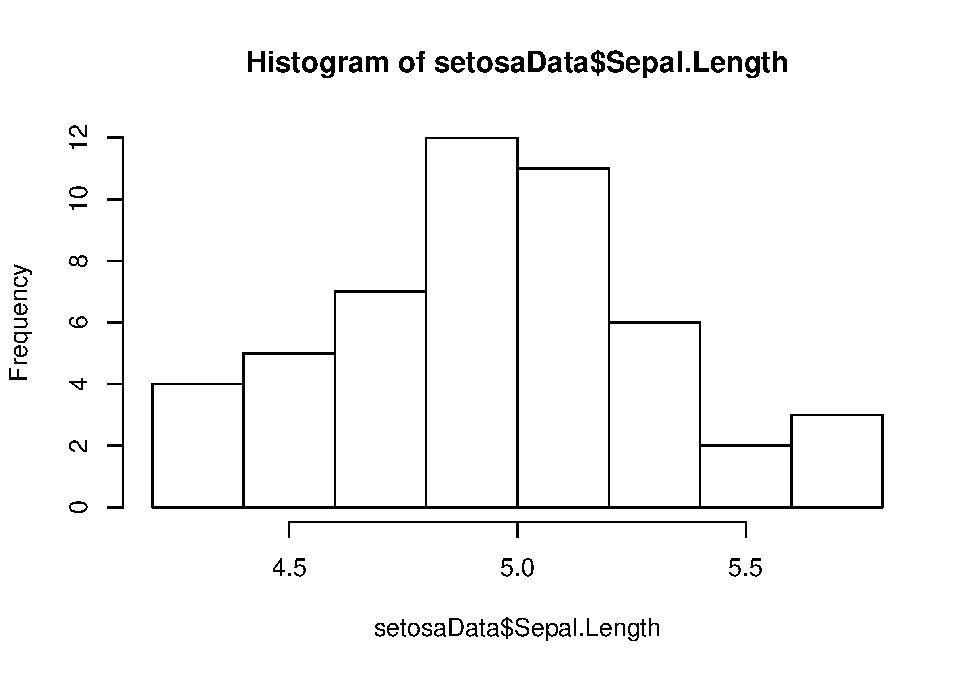
\includegraphics{worstr_files/figure-latex/unnamed-chunk-54-1.pdf}

\begin{Shaded}
\begin{Highlighting}[]
\CommentTok{# Bi-plot}
\KeywordTok{plot}\NormalTok{(setosaData}\OperatorTok{$}\NormalTok{Sepal.Width, setosaData}\OperatorTok{$}\NormalTok{Sepal.Length)}
\end{Highlighting}
\end{Shaded}

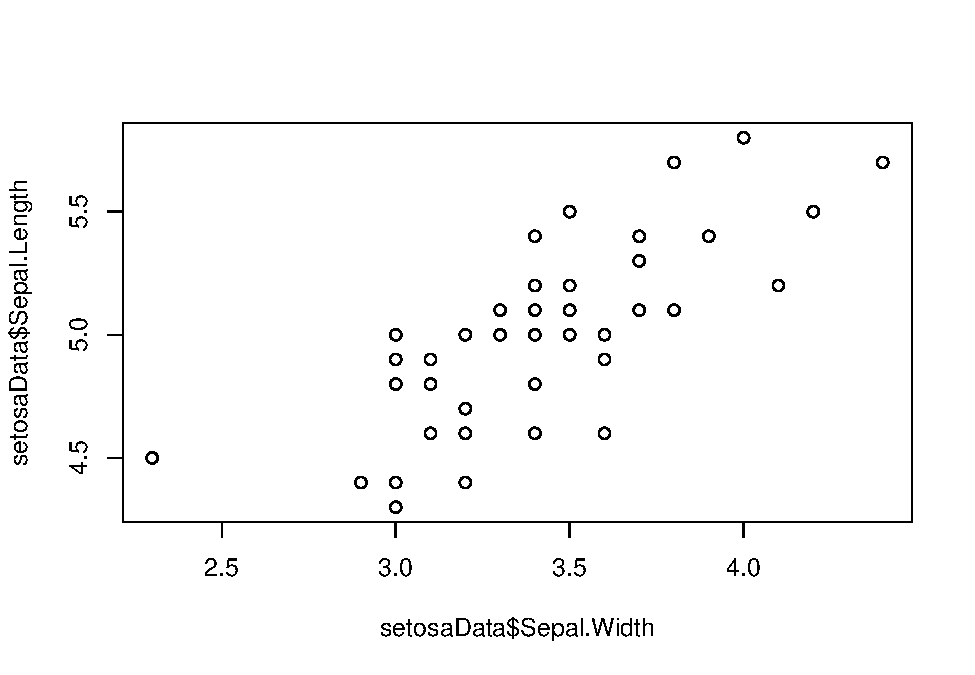
\includegraphics{worstr_files/figure-latex/unnamed-chunk-54-2.pdf}

\begin{Shaded}
\begin{Highlighting}[]
\CommentTok{# Boxplots}
\KeywordTok{boxplot}\NormalTok{(Sepal.Width }\OperatorTok{~}\StringTok{ }\NormalTok{Species, }\DataTypeTok{data =}\NormalTok{ iris)}
\end{Highlighting}
\end{Shaded}

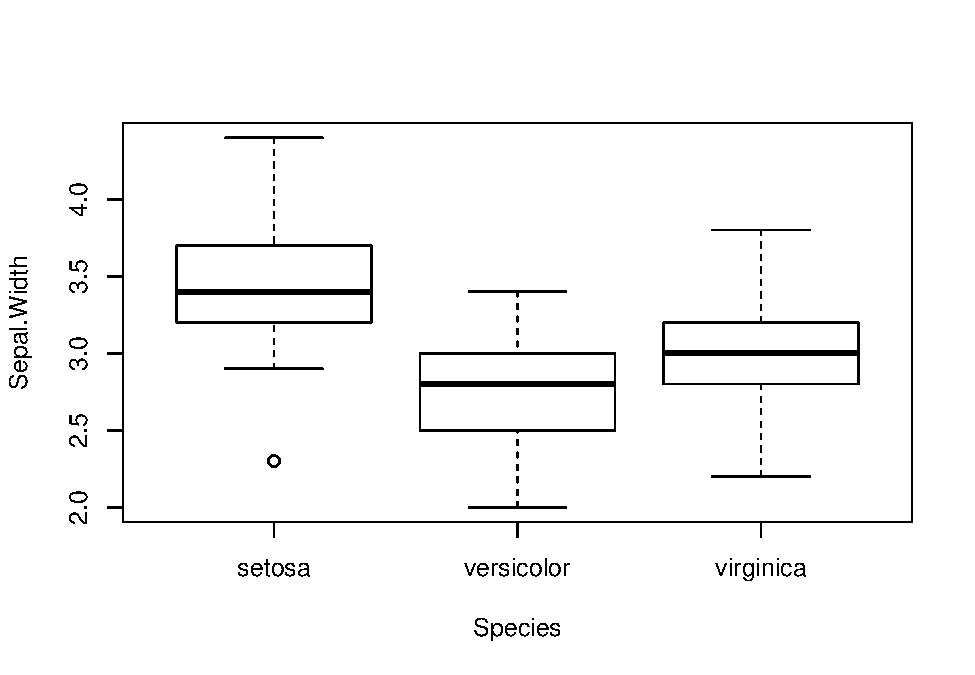
\includegraphics{worstr_files/figure-latex/unnamed-chunk-54-3.pdf}

Much, \textbf{MUCH} more of this to come as we continue.

\hypertarget{lists}{%
\section{Lists}\label{lists}}

\textbf{Lists} are the ultimate data type in R. They are actually a \href{vectors}{vector} that can hold different kinds of data, like a \protect\hyperlink{dataframes}{dataframe}. In fact, a dataframe is just a spectacularly rectangular list. Each element of a list can be any kind of object (an atomic vector, a matrix, a dataframe, or even another list!!).

Most of the real, filthy R programming relies heavily on lists. We will have to work with them at some point in this class, but we won't take a ton of time on them here.

Let's make a list- just to see how they work. Notice how our index operator has changed from \texttt{{[}\ {]}} to \texttt{{[}{[}\ {]}{]}}? And, at the highest level of organization, we have only one dimension in our list, but any given element \texttt{myList{[}{[}i{]}{]}} could hold any number of dimensions.

\begin{Shaded}
\begin{Highlighting}[]
\CommentTok{# Create an empty list with four elements}
\NormalTok{myList <-}\StringTok{ }\KeywordTok{vector}\NormalTok{(}\DataTypeTok{mode =} \StringTok{"list"}\NormalTok{, }\DataTypeTok{length =} \DecValTok{4}\NormalTok{)}

\CommentTok{# Assign some of our previously}
\CommentTok{# created objects to the elements}
\NormalTok{myList[[}\DecValTok{1}\NormalTok{]] <-}\StringTok{ }\NormalTok{a}
\NormalTok{myList[[}\DecValTok{2}\NormalTok{]] <-}\StringTok{ }\NormalTok{c}
\NormalTok{myList[[}\DecValTok{3}\NormalTok{]] <-}\StringTok{ }\NormalTok{mat}
\NormalTok{myList[[}\DecValTok{4}\NormalTok{]] <-}\StringTok{ }\NormalTok{d}
\end{Highlighting}
\end{Shaded}

Have a look at the list:

\begin{Shaded}
\begin{Highlighting}[]
\CommentTok{# Print it}
\CommentTok{# Cool, huh?}
\NormalTok{myList}
\end{Highlighting}
\end{Shaded}

\begin{verbatim}
## [[1]]
##  [1]  0.5  1.0  1.5  2.0  2.5  3.0  3.5  4.0  4.5  5.0  5.5  6.0  6.5  7.0  7.5
## [16]  8.0  8.5  9.0  9.5 10.0
## 
## [[2]]
##  [1] "a" "b" "c" "d" "a" "b" "c" "d" "a" "b" "c" "d" "a" "b" "c" "d" "a" "b" "c"
## [20] "d"
## 
## [[3]]
##        first second third
## This       1      5     9
## is         2      6    10
## a          3      7    11
## matrix     4      8    12
## 
## [[4]]
##       a      b c
## 1   0.5   0.25 a
## 2   1.0   1.00 b
## 3   1.5   2.25 c
## 4   2.0   4.00 d
## 5   2.5   6.25 a
## 6   3.0   9.00 b
## 7   3.5  12.25 c
## 8   4.0  16.00 d
## 9   4.5  20.25 a
## 10  5.0  25.00 b
## 11  5.5  30.25 c
## 12  6.0  36.00 d
## 13  6.5  42.25 a
## 14  7.0  49.00 b
## 15  7.5  56.25 c
## 16  8.0  64.00 d
## 17  8.5  72.25 a
## 18  9.0  81.00 b
## 19  9.5  90.25 c
## 20 10.0 100.00 d
\end{verbatim}

You can assign names when you create the list like we did for dataframes, too. You can do this manually, or R will do it on the fly for you. You can also reassign names to a list that yo've already created.

\begin{Shaded}
\begin{Highlighting}[]
\CommentTok{# No names by default}
\KeywordTok{names}\NormalTok{(myList)}

\CommentTok{# Give it names like we did with}
\CommentTok{# a dataframe}
\KeywordTok{names}\NormalTok{(myList) <-}\StringTok{ }\KeywordTok{c}\NormalTok{(}\StringTok{"a"}\NormalTok{, }\StringTok{"c"}\NormalTok{, }\StringTok{"mat"}\NormalTok{, }\StringTok{"d"}\NormalTok{)}

\CommentTok{# See how the names work now?}
\NormalTok{myList}

\CommentTok{# We reference these differently [[]]}
\NormalTok{myList[[}\DecValTok{1}\NormalTok{]]}

\CommentTok{# But we can still get into each object}
\CommentTok{# Play around with the numbers to see what they do!}
\NormalTok{myList[[}\DecValTok{2}\NormalTok{]][}\DecValTok{5}\NormalTok{]}

\CommentTok{# Can also reference it this way!}
\NormalTok{myList}\OperatorTok{$}\NormalTok{c[}\DecValTok{1}\NormalTok{]}
\end{Highlighting}
\end{Shaded}

Very commonly, model objects and output are stored as lists. In fact, most objects that require a large amount of diverse information in R pack it all together in one place using lists, that way we always know where to find it and how as long as the objects are documented. Conceptually, every object in R, from your workspace on down the line, is a list \textbf{AND} an element of a list. It seems like a lot to take in now, but will be very useful in the future.

\hypertarget{next2}{%
\section{Next steps}\label{next2}}

For more practice with the data structures and R functions we covered here, you can check out this walk-through of basic R commands from the How To R YouTube Channel.

In the Chapter 3(\#Chapter3), we will begin using functions from external R packages to read and work with real data.

\hypertarget{Chapter3}{%
\chapter{Working with data}\label{Chapter3}}

American shad, the best fish, lost in the data deluge. Let's figure out how to make some sense of it.

The purpose of this chapter is to get you comfortable working with data in R and give you some tools for summarizing those data in a meaningful way. This is not meant to be a comprehensive treatment of these subjects but rather an introduction to the tools that are available to you (say it with me: ``Worst Stats Text eveR''). There are a lot of tools out there and you may come up with something that works better for you once you have some basics under your belt.

Now that you have a handle on the types of data you can expect to run into in R, let's have a look at how we read and work with data that we get from the real world.

We will work with the \texttt{ctr\_fish.csv} file for Chapter 3, so you will need to download the class data sets that go with this book to play along. We will also need the \texttt{tidyverse} package, but instructions for installation are provided below because this is the first time we have downloaded and installed a package.

\hypertarget{data-read}{%
\section{Data read}\label{data-read}}

There are few things that will turn someone away from a statistical software program faster than if they can't even figure out how to get the program to read in their data. So, we are going to get it out of the way right up front!

Let's start by reading in a data file - this time we use real data.

The data are stored in a ``comma separated values'' file (\texttt{.csv} extension). This is a fairly universal format, so we read it in using the fairly universal \texttt{read.csv()} function. This would change depending on how the data were stored, or how big the data files were, but that is a topic further investigation for a later date. I probably do 95\% of my data reads using \texttt{.csv} files. We'll look at a few others later.

\textbf{Important} Remember that I am assuming your scripts are in the same directory (folder) on your computer as where you downloaded and unzipped the class data (see \href{https://danstich.github.io/stich/classes/BIOL217/software.html}{here} for reminder).

\textbf{Before you can read this file} you will need to set your working directory. For class, I will ask that you click \texttt{Session\ \textgreater{}\ Set\ Working\ Directory\ \textgreater{}\ To\ Source\ File\ Location}. This will set the working directory to wherever you have saved your code so that R can find the folder \texttt{data} and the files inside of it. You'll notice that R spits out some code in the console when you click this. You can also use that code to set a working directory in your script but that can cause \href{https://support.rstudio.com/hc/en-us/articles/200711843-Working-Directories-and-Workspaces}{all kinds of problems}, so don't do it.

\begin{Shaded}
\begin{Highlighting}[]
\CommentTok{# Start by reading in the data}
\NormalTok{am_shad <-}\StringTok{ }\KeywordTok{read.csv}\NormalTok{(}\StringTok{"data/ctr_fish.csv"}\NormalTok{)}
\end{Highlighting}
\end{Shaded}

Once you've read your data in, it's always a good idea to look at the first few lines of data to make sure nothing looks `fishy'. Ha-ha, I couldn't help myself!

These are sex-specific length and age data for American shad (\emph{Alosa sapidissima}) from the Connecticut River, USA. The data are used in models that I maintain with collaborators from NOAA Fisheries, the US Geological Survey, the US Fish and Wildlife Service, and others. The data were provided by CT Department of Energy and Environmental Protection (CTDEEP) and come from adult fish that return to the river from the ocean each year to spawn in fresh water.

You can look at the first few rows of data with the \texttt{head()} function:

\begin{Shaded}
\begin{Highlighting}[]
\CommentTok{# Look at the first 10 rows}
\KeywordTok{head}\NormalTok{(am_shad, }\DecValTok{10}\NormalTok{)}
\end{Highlighting}
\end{Shaded}

\begin{verbatim}
##    Sex Age Length yearCollected backCalculated Mass
## 1    B   1     13          2010           TRUE   NA
## 2    B   1     15          2010           TRUE   NA
## 3    B   1     15          2010           TRUE   NA
## 4    B   1     15          2010           TRUE   NA
## 5    B   1     15          2010           TRUE   NA
## 6    B   1     15          2010           TRUE   NA
## 7    B   1     16          2010           TRUE   NA
## 8    B   1     16          2010           TRUE   NA
## 9    B   1     16          2010           TRUE   NA
## 10   B   1     16          2010           TRUE   NA
\end{verbatim}

The \texttt{NA} values are supposed to be there. They are missing data.

And, don't forget about your old friend \texttt{str()} for a peek at how R sees your data. This can take care of a lot of potential problems later on.

\begin{Shaded}
\begin{Highlighting}[]
\CommentTok{# Look at the structure of the data}
\KeywordTok{str}\NormalTok{(am_shad)}
\end{Highlighting}
\end{Shaded}

\begin{verbatim}
## 'data.frame':	16946 obs. of  6 variables:
##  $ Sex           : Factor w/ 2 levels "B","R": 1 1 1 1 1 1 1 1 1 1 ...
##  $ Age           : int  1 1 1 1 1 1 1 1 1 1 ...
##  $ Length        : num  13 15 15 15 15 15 16 16 16 16 ...
##  $ yearCollected : int  2010 2010 2010 2010 2010 2010 2010 2010 2010 2010 ...
##  $ backCalculated: logi  TRUE TRUE TRUE TRUE TRUE TRUE ...
##  $ Mass          : int  NA NA NA NA NA NA NA NA NA NA ...
\end{verbatim}

There are about 17,000 observations (rows) of 6 variables (columns) in this data set. Here is a quick breakdown:

\texttt{Sex}: fish gender. \texttt{B} stands for `buck' (males), \texttt{R} stands for `roe' (females).\\

\texttt{Age}: an integer describing fish age.\\

\texttt{Length}: fish length at age (cm).\\

\texttt{yearCollected}: the year in which the fish was caught.\\

\texttt{backCalculated}: a logical indicating whether or not the length
of the fish was back-calculated from aging.\\

\texttt{Mass}: the mass of indnividual fish (in grams). Note that this is NA
for all ages that were estimated from hard structures (so all
cases for which \texttt{backCalculated\ ==\ TRUE}).

\hypertarget{quick-data-summaries}{%
\section{Quick data summaries}\label{quick-data-summaries}}

There are a number of simple ways to summarize data quickly in base R. We already looked at a few of these in previous chapters. But what about something a little more in-depth?

One quick way to look at your data is using the \texttt{summary()} function

\begin{Shaded}
\begin{Highlighting}[]
\KeywordTok{summary}\NormalTok{(am_shad)}
\end{Highlighting}
\end{Shaded}

\begin{verbatim}
##  Sex           Age            Length      yearCollected  backCalculated 
##  B:9512   Min.   :1.000   Min.   : 3.00   Min.   :2010   Mode :logical  
##  R:7434   1st Qu.:2.000   1st Qu.:31.00   1st Qu.:2011   FALSE:3046     
##           Median :3.000   Median :38.00   Median :2012   TRUE :13900    
##           Mean   :3.155   Mean   :36.39   Mean   :2012                  
##           3rd Qu.:4.000   3rd Qu.:43.00   3rd Qu.:2013                  
##           Max.   :7.000   Max.   :55.00   Max.   :2014                  
##                                                                         
##       Mass      
##  Min.   :   0   
##  1st Qu.: 900   
##  Median :1120   
##  Mean   :1173   
##  3rd Qu.:1440   
##  Max.   :3280   
##  NA's   :14115
\end{verbatim}

This is useful for getting the big-picture. For continuous variables (e.g., \texttt{Age} and \texttt{Length}) R will report some descriptive statistics like the \texttt{mean}, \texttt{median}, and quantiles. For discrete variables (e.g.~\texttt{Sex} and \texttt{backCalculated}) we get the mode (if not \texttt{factor} or \texttt{chr}) and counts of observations within each discrete level (e.g.~number of observations of \texttt{B} and \texttt{R} in the variable \texttt{Sex}).

But, this approach doesn't really give us much info.

We can create more meaningful summaries pretty easily if we install and load some packages like we talked about in \protect\hyperlink{Chapter1}{Chapter 1}, and then look at different ways of sub-setting the data with base R and some methods that might be a little more intuitive for you.

\hypertarget{subsetting-and-selecting-data}{%
\section{Subsetting and selecting data}\label{subsetting-and-selecting-data}}

Before we can make meaningful data summaries, we will probably need to re-organize our data in a logical way (through sub-setting or selected specific chunks of data). A lot of times, we do this along the way without really thinking about it.

\hypertarget{manual-subsets-and-selections}{%
\subsection{Manual subsets and selections}\label{manual-subsets-and-selections}}

We talked a little about sub-setting data with logical queries in \protect\hyperlink{Chapter2}{Chapter 2}. Now, let's refresh and take that a little further to see why we might want to do that.

First, we'll select just the data from \texttt{am\_shad} where \texttt{backCalculated} was \texttt{FALSE}. This will give us only the measured \texttt{Length} and \texttt{Mass} for each of the fish, along with their \texttt{Sex} and \texttt{yearCollected}. I'll call this new object \texttt{measured}. Remember, \texttt{am\_shad} is a data frame, so it has two dimensions when we use \texttt{{[}\ {]}} for sub-setting and these are separated by a comma, like this: \texttt{object{[}rows,\ columns{]}}. When we leave the columns blank, R knows that it should keep all of the columns.

\begin{Shaded}
\begin{Highlighting}[]
\NormalTok{measured <-}\StringTok{ }\NormalTok{am_shad[am_shad}\OperatorTok{$}\NormalTok{backCalculated }\OperatorTok{==}\StringTok{ }\OtherTok{FALSE}\NormalTok{, ]}
\end{Highlighting}
\end{Shaded}

We could do this for as many conceivable conditions in our data on which we may wish to subset, but the code can get clunky and hard to manage. For example can you imagine re-writing this if you just want to select age six roes without back-calculated lengths?

\begin{Shaded}
\begin{Highlighting}[]
\CommentTok{# Notice how we string together multiple }
\CommentTok{# conditions with "&". If these were 'or'}
\CommentTok{# we would use the vertical pipe "|"}
\NormalTok{age_}\DecValTok{6}\NormalTok{_rows_measured <-}\StringTok{ }\NormalTok{am_shad[am_shad}\OperatorTok{$}\NormalTok{backCalculated }\OperatorTok{==}\StringTok{ }\OtherTok{FALSE} \OperatorTok{&}\StringTok{ }
\StringTok{                                 }\NormalTok{am_shad}\OperatorTok{$}\NormalTok{Sex }\OperatorTok{==}\StringTok{ "R"} \OperatorTok{&}
\StringTok{                                 }\NormalTok{am_shad}\OperatorTok{$}\NormalTok{Age }\OperatorTok{==}\StringTok{ }\DecValTok{6}\NormalTok{, ]}
\end{Highlighting}
\end{Shaded}

\hypertarget{subsetting-and-summaries-in-base-r}{%
\subsection{Subsetting and summaries in base R}\label{subsetting-and-summaries-in-base-r}}

This notation can be really confusing to folks who are just trying to learn a new programming language. Because of that, there are great functions like \texttt{subset()} available that are more intuitive (but less clear to programmers). You could also subset the data using the following code:

\begin{Shaded}
\begin{Highlighting}[]
\NormalTok{measured <-}\StringTok{ }\KeywordTok{subset}\NormalTok{(am_shad, backCalculated }\OperatorTok{==}\StringTok{ }\OtherTok{FALSE}\NormalTok{)}
\end{Highlighting}
\end{Shaded}

We could also get our age-six females from the previous example using this approach, and at least the code is a little cleaner:

\begin{Shaded}
\begin{Highlighting}[]
\NormalTok{age_}\DecValTok{6}\NormalTok{_roes_measured <-}\StringTok{ }\KeywordTok{subset}\NormalTok{(am_shad,}
\NormalTok{                              backCalculated }\OperatorTok{==}\StringTok{ }\OtherTok{FALSE} \OperatorTok{&}
\StringTok{                                }\NormalTok{Sex }\OperatorTok{==}\StringTok{ "R"} \OperatorTok{&}
\StringTok{                                }\NormalTok{Age }\OperatorTok{==}\StringTok{ }\DecValTok{6}
\NormalTok{                              )}
\end{Highlighting}
\end{Shaded}

Both do the same thing, but we'll see later that using \texttt{subset} is preferable if we plan on chaining together a bunch of data manipulation commands using pipes (\texttt{\%\textgreater{}\%}).

Next, we might be interested to know how many fish we have represented in each \texttt{Sex}. We can find this out using the \texttt{table} function in base R:

\begin{Shaded}
\begin{Highlighting}[]
\CommentTok{# Here, I use the column name because}
\CommentTok{# we just want all observations of a single}
\CommentTok{# variable. Be careful switching between names,}
\CommentTok{# numbers, and $names!}
\KeywordTok{table}\NormalTok{(measured[}\StringTok{'Sex'}\NormalTok{])}
\end{Highlighting}
\end{Shaded}

\begin{verbatim}
## 
##    B    R 
## 1793 1253
\end{verbatim}

We see that we have \texttt{1793} females and \texttt{1253} males.

We can also get tallies of the number of fish in each \texttt{Age} for each \texttt{Sex} if we would like to see that:

\begin{Shaded}
\begin{Highlighting}[]
\KeywordTok{table}\NormalTok{(measured}\OperatorTok{$}\NormalTok{Sex, measured}\OperatorTok{$}\NormalTok{Age)}
\end{Highlighting}
\end{Shaded}

\begin{verbatim}
##    
##       3   4   5   6   7
##   B 255 848 579 108   3
##   R   0 361 658 220  14
\end{verbatim}

But, what if we wanted to calculate some kind of summary statistic, like a \texttt{mean} and report that by group?

For our age-6 females example, it would look like this:

\begin{Shaded}
\begin{Highlighting}[]
\NormalTok{age_}\DecValTok{6}\NormalTok{_roes_measured <-}\StringTok{ }\KeywordTok{subset}\NormalTok{(am_shad,}
\NormalTok{                              backCalculated }\OperatorTok{==}\StringTok{ }\OtherTok{FALSE} \OperatorTok{&}
\StringTok{                                }\NormalTok{Sex }\OperatorTok{==}\StringTok{ "R"} \OperatorTok{&}
\StringTok{                                }\NormalTok{Age }\OperatorTok{==}\StringTok{ }\DecValTok{6}
\NormalTok{                              )}

\NormalTok{age_}\DecValTok{6}\NormalTok{_female_mean <-}\StringTok{ }\KeywordTok{mean}\NormalTok{(age_}\DecValTok{6}\NormalTok{_roes_measured}\OperatorTok{$}\NormalTok{Length)}
\end{Highlighting}
\end{Shaded}

Again, we could do this manually, but would require a lot of code for a simple calculation if we use the methods above all by themselves to get these for each age group of roes.

We would basically just copy-and-paste the code over and over to force R into making the data summaries we need. Nothing wrong with this approach, and it certainly has its uses for simple summaries, but it can be cumbersome and redundant. It also fills your workspace up with tons of objects that are hard to keep track of and that will cause your code-completion suggestions to be \emph{wicked} annoying in RStudio.

That usually means there is a better way to write the code\ldots{}

\hypertarget{tidyverse}{%
\subsection{Subsetting and summaries in the tidyverse}\label{tidyverse}}

Long ago, when I was still a noOb writing R code with a stand-alone text editor and a console there were not a ton of packages available for the express purpose of cleaning up data manipulation in R. The one I relied on most heavily was the \texttt{plyr} package. Since then, R has grown and a lot of these functions have been gathered under the umbrella of the \href{https://www.tidyverse.org/packages/}{tidyverse}, which is a collection of specific R packages designed to make the whole process less painful. These include packages like \texttt{dplyr} (which replaced \texttt{plyr}) and others that are designed to work together with similar syntax to make data science (for us, data manipulation and presentation) a lot cleaner and better standardized. We will rely heavily on packages in the tidyverse throughout this book.

Before we can work with these packages, however, we need to install them - something we haven't talked about yet! Most of the critical R packages are hosted through the Comprehensive R Archive Network, or \href{https://cran.r-project.org/}{CRAN}. Still, tons of others are available for installation from hosting services like GitHub and GitLab.

If you haven't seen it yet, \href{https://www.youtube.com/watch?v=u1r5XTqrCTQ}{here} is a three-minute video explaining how to install packages using RStudio. \textbf{Watch it. Please.}

It is also easy to install packages by running a line of code in the console. We could install each of the packages in the tidyverse separately. But we can also get all of them at once because they are all packaged together, too.

Follow the instructions in the YouTube link above, or install the package from the command line:

\begin{Shaded}
\begin{Highlighting}[]
\KeywordTok{install.packages}\NormalTok{(}\StringTok{'tidyverse'}\NormalTok{)}
\end{Highlighting}
\end{Shaded}

Once we have installed these packages, we can use the functions in them to clean up our data manipulation pipeline and get some really useful information.

\hypertarget{better-data-summaries}{%
\section{Better data summaries}\label{better-data-summaries}}

Now, we'll look at some slightly more advanced summaries. Start by loading the \texttt{dplyr} package into your R session with the following code.

\begin{Shaded}
\begin{Highlighting}[]
\KeywordTok{library}\NormalTok{(dplyr)}
\end{Highlighting}
\end{Shaded}

We can use functions from the \texttt{dplyr} package to calculate mean \texttt{Length} of fish for each combination of \texttt{Sex} and \texttt{Age} group much more easily than we did for a single group above.

First, we group the data in \texttt{measured} data frame that we created previously using the \texttt{group\_by} function. For this, we just need to give R the data frame and the variables by which we would like to group:

\begin{Shaded}
\begin{Highlighting}[]
\NormalTok{g_lengths <-}\StringTok{ }\KeywordTok{group_by}\NormalTok{(measured, Sex, Age)}
\end{Highlighting}
\end{Shaded}

This doesn't change how we see the data much (it gets converted to a \href{https://tibble.tidyverse.org/\#:~:text=A\%20tibble\%2C\%20or\%20tbl_df\%20\%2C\%20is,modern\%20reimagining\%20of\%20the\%20data.\&text=Tibbles\%20are\%20data.,a\%20variable\%20does\%20not\%20exist}{\texttt{tibble}}), just how R sees it.

Next, we summarize the variable \texttt{Length} by \texttt{Sex} and \texttt{Age} using the \texttt{summarize} function:

\begin{Shaded}
\begin{Highlighting}[]
\NormalTok{sum_out <-}\StringTok{ }\KeywordTok{summarize}\NormalTok{(g_lengths, }\DataTypeTok{avg =} \KeywordTok{mean}\NormalTok{(Length))}

\KeywordTok{head}\NormalTok{(sum_out)}
\end{Highlighting}
\end{Shaded}

\begin{verbatim}
## # A tibble: 6 x 3
## # Groups:   Sex [2]
##   Sex     Age   avg
##   <fct> <int> <dbl>
## 1 B         3  38.1
## 2 B         4  40.5
## 3 B         5  42.0
## 4 B         6  43.4
## 5 B         7  46.8
## 6 R         4  45.0
\end{verbatim}

Wow! That was super-easy!

Finally, to make things even more streamlined, we can chain all of these operations together using the \texttt{\%\textgreater{}\%} function from \texttt{magrittr}. This really cleans up the code and gives us small chunks of code that are easier to read than the dozens of lines of code it would take to do this manually.

\begin{Shaded}
\begin{Highlighting}[]
\CommentTok{# This will do it all at once!}
\NormalTok{sum_out <-}\StringTok{ }\CommentTok{# Front-end object assignment}
\StringTok{  }\NormalTok{measured }\OperatorTok\StringTok{ }\CommentTok{# Pass measured to the group_by function}
\StringTok{  }\KeywordTok{group_by}\NormalTok{(Sex, Age) }\OperatorTok\StringTok{ }\CommentTok{# Group by Sex and age and pass to summarize}
\StringTok{  }\KeywordTok{summarize}\NormalTok{(}\DataTypeTok{avg =} \KeywordTok{mean}\NormalTok{(Length))}
\end{Highlighting}
\end{Shaded}

We could also assign the output to a variable at the end, whichever is easier for you to read:

\begin{Shaded}
\begin{Highlighting}[]
\NormalTok{  measured }\OperatorTok\StringTok{ }\CommentTok{# Pass measured to the group_by function}
\StringTok{  }\KeywordTok{group_by}\NormalTok{(Sex, Age) }\OperatorTok\StringTok{ }\CommentTok{# Group by Sex and age and pass to summarize}
\StringTok{  }\KeywordTok{summarize}\NormalTok{(}\DataTypeTok{avg =} \KeywordTok{mean}\NormalTok{(Length)) ->}\StringTok{ }\NormalTok{sim_out }\CommentTok{# Back-end object assignment}
\end{Highlighting}
\end{Shaded}

And, it is really easy to get multiple summaries out like this at once:

\begin{Shaded}
\begin{Highlighting}[]
\NormalTok{sum_out <-}
\StringTok{  }\NormalTok{measured }\OperatorTok\StringTok{ }
\StringTok{  }\KeywordTok{group_by}\NormalTok{(Sex, Age) }\OperatorTok\StringTok{ }
\StringTok{  }\KeywordTok{summarize}\NormalTok{(}\DataTypeTok{avg =} \KeywordTok{mean}\NormalTok{(Length), }\DataTypeTok{s.d. =} \KeywordTok{sd}\NormalTok{(Length))}

\KeywordTok{head}\NormalTok{(sum_out)}
\end{Highlighting}
\end{Shaded}

\begin{verbatim}
## # A tibble: 6 x 4
## # Groups:   Sex [2]
##   Sex     Age   avg  s.d.
##   <fct> <int> <dbl> <dbl>
## 1 B         3  38.1  2.75
## 2 B         4  40.5  2.70
## 3 B         5  42.0  2.29
## 4 B         6  43.4  2.09
## 5 B         7  46.8  1.61
## 6 R         4  45.0  2.65
\end{verbatim}

Isn't that slick? Just think how long that would have taken most of us in Excel!

This is just one example of how functions in packages can make your life easier and your code more efficient. Now that we have the basics under our belts, lets move on to how we create new variables.

\hypertarget{creating-new-variables}{%
\section{Creating new variables}\label{creating-new-variables}}

There are basically two ways to create new variables: we can modify an existing variable (groups or formulas), or we can simulate new values for that variable (random sampling.)

If we have a formula that relates two variables, we could predict one based on the other deterministically.

For example, I have fit a length-weight regression to explain the relationship between \texttt{Length} and \texttt{Mass} using the \texttt{am\_shad} data we've worked with in previous sections.

This relationship looks like your old friend \(y = mx + b\), the equation for a line, but we log10-transform both of the variables before fitting the line (more to come later in the class). Using this relationship, we can predict our \textbf{independent variable} (\texttt{Mass}) from our \textbf{dependent variable} (\texttt{Length}) if we plug in new values for \texttt{Length} and the \textbf{parameters} of the line.

In this case, I know that \texttt{m} = 3.0703621, and \texttt{b} = -1.9535405.

If I plug these numbers in to the equation above, I can predict \texttt{log10(Mass)} for new lengths \texttt{log10(Length)}:

\(log_{10}Mass = 3.0703621 \cdot log_{10}Length - 1.9535405\)

In R, this looks like:

\begin{Shaded}
\begin{Highlighting}[]
\CommentTok{# Parameters from length-weight regression}
\NormalTok{m <-}\StringTok{ }\FloatTok{3.0703621}
\NormalTok{b <-}\StringTok{ }\FloatTok{1.9535405}

\CommentTok{# Make a sequence of new lengths based on range in data,}
\CommentTok{# then take the log of the whole thing all at once.}
\NormalTok{log_length <-}\StringTok{ }\KeywordTok{log10}\NormalTok{( }\KeywordTok{seq}\NormalTok{(}\KeywordTok{min}\NormalTok{(am_shad}\OperatorTok{$}\NormalTok{Length), }\KeywordTok{max}\NormalTok{(am_shad}\OperatorTok{$}\NormalTok{Length), }\DecValTok{1}\NormalTok{) )}

\CommentTok{# Calculate a new thing (log10_mass) using parameters for line}
\CommentTok{# and sequence of new log10_length.}
\NormalTok{log_mass <-}\StringTok{ }\NormalTok{m }\OperatorTok{*}\StringTok{ }\NormalTok{log_length }\OperatorTok{+}\StringTok{ }\NormalTok{b}

\CommentTok{# Plot the prediction}
\KeywordTok{plot}\NormalTok{(}\DataTypeTok{x =}\NormalTok{ log_length, }\DataTypeTok{y =}\NormalTok{ log_mass, }\DataTypeTok{type =} \StringTok{"l"}\NormalTok{)}
\end{Highlighting}
\end{Shaded}

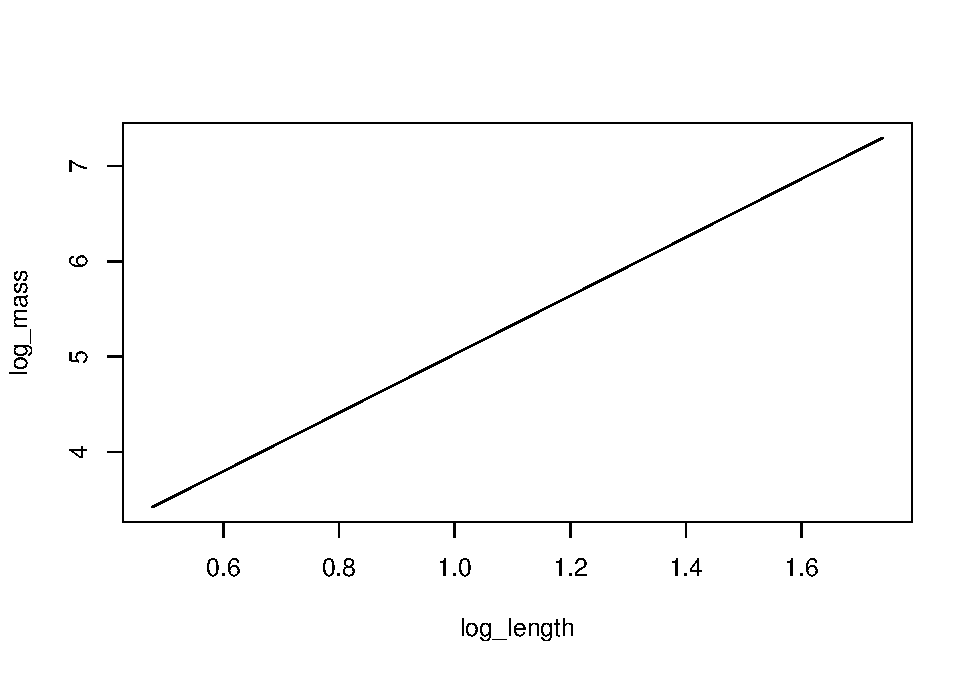
\includegraphics{worstr_files/figure-latex/unnamed-chunk-77-1.pdf}

\hypertarget{data-simulation}{%
\section{Data simulation}\label{data-simulation}}

The point of simulation is usually to account for uncertainty in some process (i.e.~we could just pick a single value if we knew it). This is almost always done based on probability. There are a number of ways we could do this. One is by drawing from some probability distribution that we have described, and the other is by randomly sampling data that we already have.

\hypertarget{random-sub-samples-from-a-dataset}{%
\subsection{Random sub-samples from a dataset}\label{random-sub-samples-from-a-dataset}}

Let's say we want to take random samples from our huge data set so we can fit models to a subset of data and then use the rest of our data for model validation in weeks to come.

We have around 17,000 observations in the \texttt{am\_shad} data set. But, what if we wanted to know what it would look like if we only had 100 samples from the same population?

First, tell R how many samples you want.

\begin{Shaded}
\begin{Highlighting}[]
\NormalTok{n_samples <-}\StringTok{ }\DecValTok{100}
\end{Highlighting}
\end{Shaded}

Now let's take two samples of 100 fish from our dataframe to see how they compare:

\begin{Shaded}
\begin{Highlighting}[]
\CommentTok{# Randomly sample 100 rows of data from our data frame two different}
\CommentTok{# times to see the differences}
\NormalTok{samp1 <-}\StringTok{ }\NormalTok{am_shad[}\KeywordTok{sample}\NormalTok{(}\KeywordTok{nrow}\NormalTok{(am_shad), }\DataTypeTok{size =}\NormalTok{ n_samples, }\DataTypeTok{replace =} \OtherTok{FALSE}\NormalTok{), ]}
\NormalTok{samp2 <-}\StringTok{ }\NormalTok{am_shad[}\KeywordTok{sample}\NormalTok{(}\KeywordTok{nrow}\NormalTok{(am_shad), }\DataTypeTok{size =}\NormalTok{ n_samples, }\DataTypeTok{replace =} \OtherTok{FALSE}\NormalTok{), ]}

\CommentTok{# We can look at them with our histograms}
\KeywordTok{par}\NormalTok{(}\DataTypeTok{mfrow =} \KeywordTok{c}\NormalTok{(}\DecValTok{1}\NormalTok{, }\DecValTok{2}\NormalTok{))}
\KeywordTok{hist}\NormalTok{(samp1}\OperatorTok{$}\NormalTok{Length, }\DataTypeTok{main =} \StringTok{""}\NormalTok{, }\DataTypeTok{ylim =} \KeywordTok{c}\NormalTok{(}\DecValTok{0}\NormalTok{, }\DecValTok{30}\NormalTok{))}
\KeywordTok{hist}\NormalTok{(samp2}\OperatorTok{$}\NormalTok{Length, }\DataTypeTok{main =} \StringTok{""}\NormalTok{, }\DataTypeTok{ylim =} \KeywordTok{c}\NormalTok{(}\DecValTok{0}\NormalTok{, }\DecValTok{30}\NormalTok{))}
\end{Highlighting}
\end{Shaded}

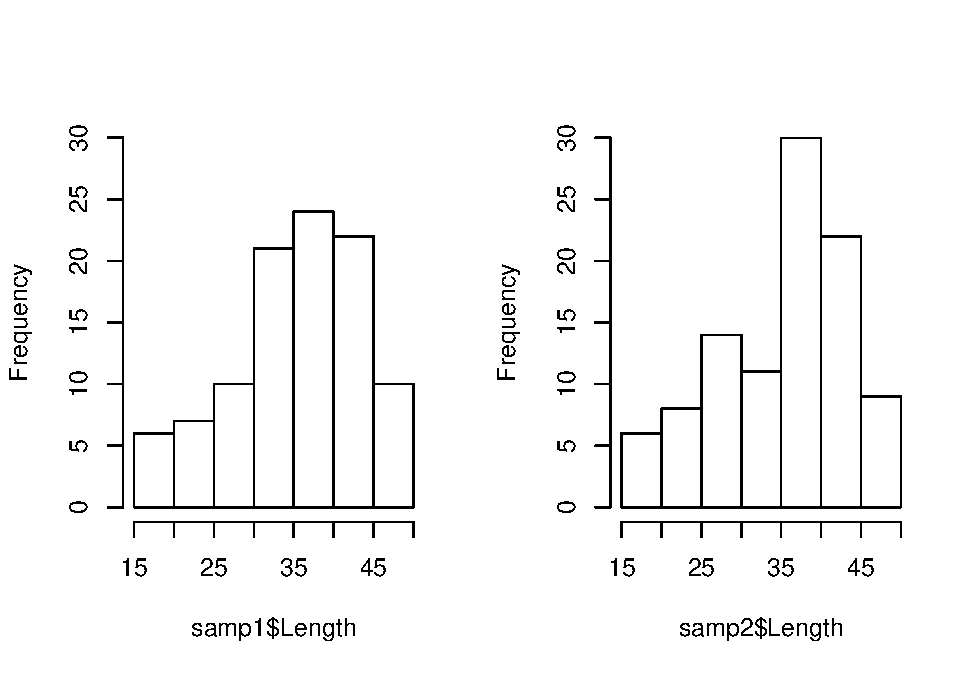
\includegraphics{worstr_files/figure-latex/unnamed-chunk-79-1.pdf}
*If you are struggling to get your plotting window back to ``normal'' after this, you can either click the broom button in your ``Plots'' window, or you can run the following code for now:

\hypertarget{stochastic}{%
\subsection{Stochastic simulation}\label{stochastic}}

Now, instead of sampling our data let's say we have some distribution from which we would like sample. So, let's make a distribution.

We will start with the normal, and we can move into others when we talk about probability distributions and sample statistics in \protect\hyperlink{Chapter5}{Chapter 5}. For this, we will use the distribution of American shad lengths for age-6 females because it approximates a normal distribution. We will calculate the \texttt{mean} and \texttt{sd} because those are the parameters of the normal distribution.

Start by looking at the size distribution for age 6 females. We use the tidy workflow here with really awful default graphics (more to come in \protect\hyperlink{Chapter4}{Chapter 4}), but we add two arguments to our \texttt{subset} call. We want to select only the variable \texttt{Length} from \texttt{am\_shad}, and we want to drop all other information so we can send the output straight to the \texttt{hist()} function as a vector.

\begin{Shaded}
\begin{Highlighting}[]
\NormalTok{am_shad }\OperatorTok
\StringTok{  }\KeywordTok{subset}\NormalTok{(Age }\OperatorTok{==}\StringTok{ }\DecValTok{6} \OperatorTok{&}\StringTok{ }\NormalTok{Sex }\OperatorTok{==}\StringTok{ "R"}\NormalTok{, }\DataTypeTok{select=}\StringTok{'Length'}\NormalTok{, }\DataTypeTok{drop=}\OtherTok{TRUE}\NormalTok{) }\OperatorTok
\StringTok{   }\KeywordTok{hist}\NormalTok{(}\DataTypeTok{main =} \StringTok{""}\NormalTok{)}
\end{Highlighting}
\end{Shaded}

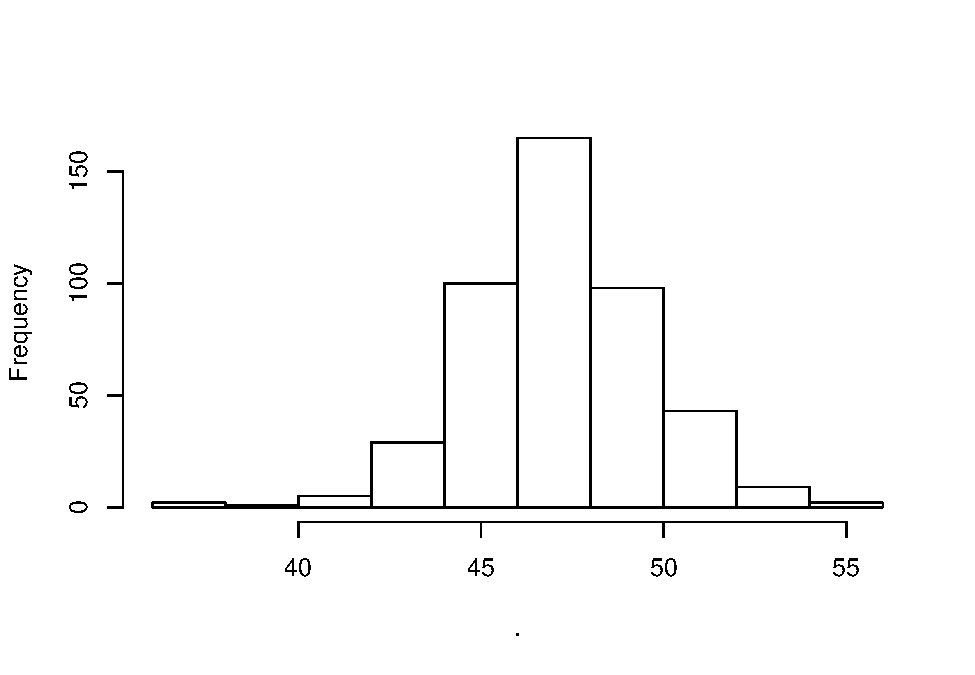
\includegraphics{worstr_files/figure-latex/unnamed-chunk-81-1.pdf}

Now, let's calculate the \texttt{mean} and \texttt{sd} of \texttt{Length} for age 6 females.

\begin{Shaded}
\begin{Highlighting}[]
\CommentTok{# Calculate the mean Length }
\NormalTok{x_bar <-}\StringTok{ }\NormalTok{am_shad }\OperatorTok
\StringTok{  }\KeywordTok{subset}\NormalTok{(Age }\OperatorTok{==}\StringTok{ }\DecValTok{6} \OperatorTok{&}\StringTok{ }\NormalTok{Sex }\OperatorTok{==}\StringTok{ "R"}\NormalTok{, }\DataTypeTok{select=}\StringTok{'Length'}\NormalTok{, }\DataTypeTok{drop=}\OtherTok{TRUE}\NormalTok{) }\OperatorTok
\StringTok{  }\NormalTok{mean}

\CommentTok{# Calculate standard deviation of Length}
\NormalTok{sigma <-}\StringTok{ }\NormalTok{am_shad }\OperatorTok
\StringTok{  }\KeywordTok{subset}\NormalTok{(Age }\OperatorTok{==}\StringTok{ }\DecValTok{6} \OperatorTok{&}\StringTok{ }\NormalTok{Sex }\OperatorTok{==}\StringTok{ "R"}\NormalTok{, }\DataTypeTok{select=}\StringTok{'Length'}\NormalTok{, }\DataTypeTok{drop=}\OtherTok{TRUE}\NormalTok{) }\OperatorTok
\StringTok{  }\NormalTok{sd}
\end{Highlighting}
\end{Shaded}

Note that we could also use the \texttt{filter()} function from the \texttt{dplyr} package for this job, and for big data sets it would be a lot faster for un-grouped data.

Now, we can use the mean and standard deviation to randomly sample our normal distribution of lengths.

\begin{Shaded}
\begin{Highlighting}[]
\CommentTok{# Take a random sample from a normal distribution}
\NormalTok{length_sample <-}\StringTok{ }\KeywordTok{rnorm}\NormalTok{(}\DataTypeTok{n =} \DecValTok{10000}\NormalTok{, }\DataTypeTok{mean =}\NormalTok{ x_bar, }\DataTypeTok{sd =}\NormalTok{ sigma)}

\CommentTok{# Plot the sample to see if it is a normal- YAY it is!}
\KeywordTok{hist}\NormalTok{(length_sample,}
  \DataTypeTok{col =} \StringTok{"gray"}\NormalTok{,}
  \DataTypeTok{main =} \StringTok{""}\NormalTok{,}
  \DataTypeTok{xlab =} \StringTok{"Forklength (cm)"}
\NormalTok{)}
\end{Highlighting}
\end{Shaded}

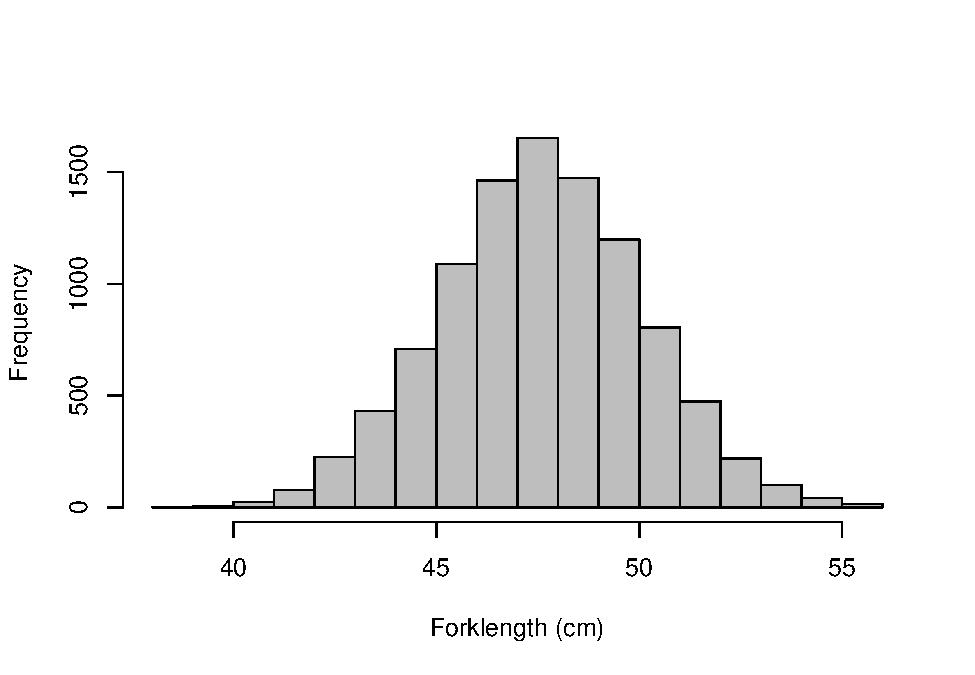
\includegraphics{worstr_files/figure-latex/unnamed-chunk-83-1.pdf}
We've add a couple of new arguments to the histogram call to make it a little less ugly here. In \protect\hyperlink{Chapter4}{Chapter 4} we are going to ramp it up and play with some plots!

\hypertarget{next3}{%
\section{Next steps}\label{next3}}

In this chapter, we provided a general overview of our work flow when it comes to reading in data and manipulating them to get useful summaries. In \protect\hyperlink{Chapter4}{Chapter 4} we will use these processes to help us visualize important trends in these summaries before we begin working with descriptive statistics and sampling distributions in \protect\hyperlink{Chapter5}{Chapter 5}.

\hypertarget{Chapter4}{%
\chapter{Plotting and graphics}\label{Chapter4}}

Sweet graphs, right? Want to learn how to make them? Okay, but baby steps here, alright?.

In this Chapter we will walk through plotting in R, both with the base graphic utilities that come with R, and the \texttt{ggplot2} package from the \texttt{tidyverse} that has taken over the world (er, revolutionized how we write R code). Both of these are actually great to work with for different reasons. The base graphics are built-in, powerful, and give you 100\% full control over your graphic environment. The \texttt{ggplot2} library (and a million packages that people have written to work with it) takes these to a new level in terms of functionality and 95\% of the time it will do exactly what you need. That other 5\% of the time it is really great to be able to fall back on the base graphics.

For the examples in this chapter, we'll work with the water quality data contained in \texttt{physical.csv}. You will need to download the class data sets that go with this book to play along if you have not already (click \href{https://danstich.github.io/stich/classes/BIOL217/software.html}{here} for instructions from the course website). But, you should have downloaded those to complete the examples in \protect\hyperlink{Chapter2}{Chapter 2}.

We will walk through histograms, scatter plots, line graphs, and boxplots in base graphics and \texttt{ggplot2} in this Chapter. Later in the book, we will add examples of how to plot predictions from statistical models alongside raw data using these same tools.

If you installed the \texttt{tidyverse} successfully in \protect\hyperlink{tidyverse}{Chapter 3}, then you can load all the packages we'll need by including \texttt{library(tidyverse)} at the start of your script:

\begin{Shaded}
\begin{Highlighting}[]
\CommentTok{# Chapter 4 Lecture module}

\CommentTok{# Package load}
\KeywordTok{library}\NormalTok{(tidyverse) }

\CommentTok{# 4.2 Plotting with base R ----}
\CommentTok{# ...}
\end{Highlighting}
\end{Shaded}

\hypertarget{plots-matter-as-much-as-stats}{%
\section{Plots matter as much as stats}\label{plots-matter-as-much-as-stats}}

Before we get started:

\begin{enumerate}
\def\labelenumi{\arabic{enumi}.}
\item
  There are few statistical tests that hold intuitive meaning to our readers. The ability to present information in a visually meaningful way to the reader can help to make the interpretation of your science crystal clear without having to worry about whether or not your reader has the faculties to interpret the results of some fancy statistical test that \emph{you} think is cool.
\item
  Effects and effect sizes are often (if not always) more important than the ability to detect `significant' differences. If you can present clear evidence that some treatment or manipulation confers a biologically meaningful change in a visual way alongside these tests, you can provide a much stronger body of evidence with which to argue your case.
\item
  There are a few graphical tools that are very useful for basic data exploration, diagnostics, etc., that can make your life a lot easier for data analysis and interpretation. They can also help you decide whether something has gone terribly wrong.
\end{enumerate}

The takeaway here is: \emph{don't make shitty graphs}.

\hypertarget{base-graphics}{%
\section{Plotting with base R}\label{base-graphics}}

Let's look at a few simple types of plots in R. The default graphics in R are not much to look at. But, there are a \textbf{ton} of ways to modify these plots, and the user (that's you!) can build plots from the ground up if needed.

One of the great things about base graphics is that many of the plot types take the same, or similar arguments that are all based on shared graphical parameters.

You can access the help file for these shared graphical parameters by running \texttt{?pars} in the console. We will use many of these in the sections that follow.

\hypertarget{histograms}{%
\subsection{Histograms}\label{histograms}}

Let's start with the histogram function that we began playing with at the end of \protect\hyperlink{stochastic}{Chapter 3}.

The \texttt{hist()} function plots a histogram but it actually does a whole lot more than just that. Like other plotting utilities, it can take a wide variety of arguments and it actually does some basic data analysis behind the scenes. All of the arguments are optional or have default values with the exception of the data that we want to plot (a numeric variable). This is the case for most plotting functions in the base graphics for R.

Start by reading in the data contained within the \texttt{physical.csv} file from the class data folder. Remember, I am assuming that your code is inside of a folder that also contains your class data folder that you named \href{https://danstich.github.io/stich/classes/BIOL217/software.html}{\texttt{data}}.

\begin{Shaded}
\begin{Highlighting}[]
\CommentTok{# I added stringsAsFactors = FALSE to read in all}
\CommentTok{# text strings as `chr`.}
\NormalTok{ otsego <-}\StringTok{ }\KeywordTok{read.csv}\NormalTok{(}\StringTok{"data/physical.csv"}\NormalTok{, }\DataTypeTok{stringsAsFactors =} \OtherTok{FALSE}\NormalTok{)}
\end{Highlighting}
\end{Shaded}

These are data collected each year from Otsego Lake by students, staff, and faculty at the SUNY Oneonta Biological Field Station in Cooperstown, NY, USA. The data set includes temperature (°C), pH, dissolved oxygen, and specific conductance measurements from a period of about 40 years. There are all kinds of cool spatial and seasonal patterns in the data that we can look at. We will use \texttt{temperature} for the examples that follow.

Make a histogram of temperature across all depths and dates just to see what we are working with here:

\begin{Shaded}
\begin{Highlighting}[]
\KeywordTok{hist}\NormalTok{(otsego}\OperatorTok{$}\NormalTok{temp)}
\end{Highlighting}
\end{Shaded}

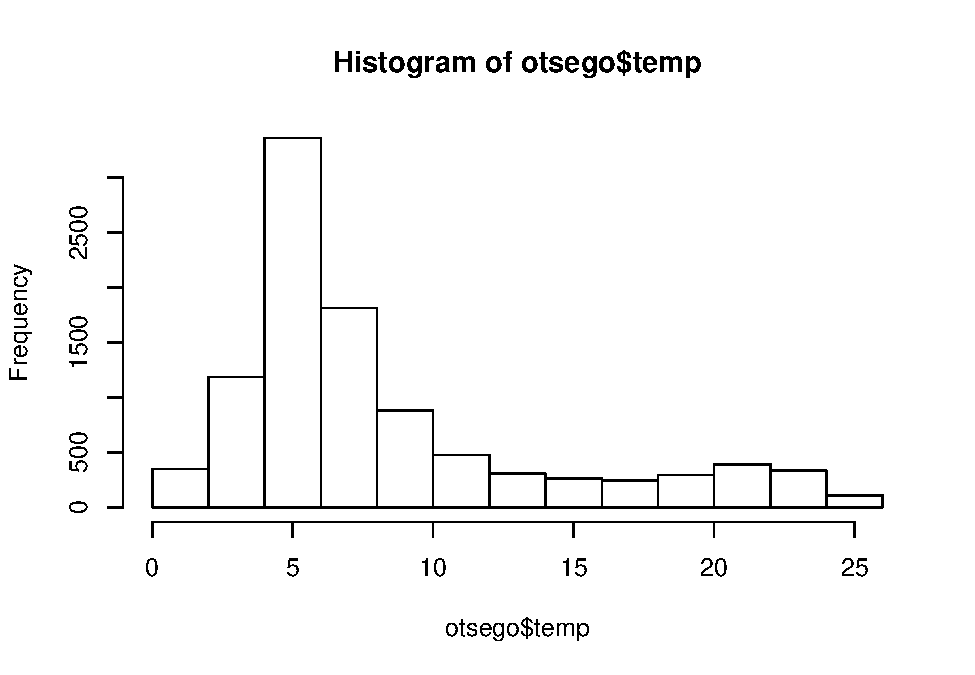
\includegraphics{worstr_files/figure-latex/unnamed-chunk-86-1.pdf}

The default histogram in base graphics leaves much to be desired. Thankfully, it is easy to modify the look of these figures. For example, we can add labels to the x and y-axis using \texttt{xlab} and \texttt{ylab}, and we can give the histogram a meaningful title by adding \texttt{main\ =\ ...} to the \texttt{hist()} call or remove it completely by saying \texttt{main\ =\ ""}.

\begin{Shaded}
\begin{Highlighting}[]
\KeywordTok{hist}\NormalTok{(otsego}\OperatorTok{$}\NormalTok{temp, }\DataTypeTok{xlab =} \StringTok{"Temperature"}\NormalTok{, }\DataTypeTok{ylab =} \StringTok{"Frequency"}\NormalTok{, }\DataTypeTok{main=}\StringTok{""}\NormalTok{)}
\end{Highlighting}
\end{Shaded}

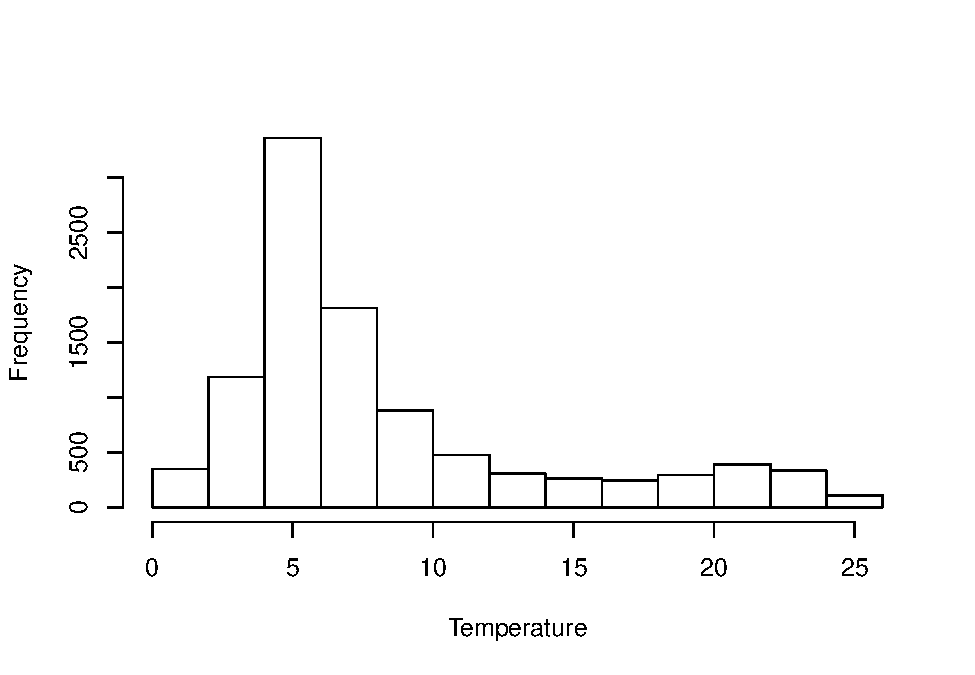
\includegraphics{worstr_files/figure-latex/unnamed-chunk-87-1.pdf}

We can make the axes cross at zero if we are concerned about that. We need to do this by specifying \texttt{yaxt\ =\ "n"}, \texttt{xaxt\ =\ "n"} in the \texttt{hist()} call and then follow up by telling R exactly where to start each of the axes. In this example, I also add some changes to the color of the bars (\texttt{col}) and the color of the borders (\texttt{border}). Finally, I fix the x- and y-axis scales so I know where they'll start.

\begin{Shaded}
\begin{Highlighting}[]
\CommentTok{# Make the histogram}
\KeywordTok{hist}\NormalTok{(otsego}\OperatorTok{$}\NormalTok{temp,}
     \DataTypeTok{xlab =} \StringTok{"Temperature"}\NormalTok{,}
     \DataTypeTok{ylab =} \StringTok{"Frequency"}\NormalTok{,}
     \DataTypeTok{main =} \StringTok{""}\NormalTok{,}
     \DataTypeTok{xaxt =} \StringTok{"n"}\NormalTok{,}
     \DataTypeTok{yaxt =} \StringTok{"n"}\NormalTok{,}
     \DataTypeTok{col =} \StringTok{"gray87"}\NormalTok{,}
     \DataTypeTok{border =} \StringTok{"white"}\NormalTok{,}
     \DataTypeTok{xlim =} \KeywordTok{c}\NormalTok{(}\DecValTok{0}\NormalTok{, }\DecValTok{30}\NormalTok{),}
     \DataTypeTok{ylim =} \KeywordTok{c}\NormalTok{(}\DecValTok{0}\NormalTok{, }\DecValTok{3500}\NormalTok{)}
\NormalTok{     )}

\CommentTok{# Add an x-axis going from zero to thirty degrees}
\CommentTok{# in increments of 2 degrees and start it at zero}
\KeywordTok{axis}\NormalTok{(}\DataTypeTok{side =} \DecValTok{1}\NormalTok{, }\DataTypeTok{at =} \KeywordTok{seq}\NormalTok{(}\DataTypeTok{from =} \DecValTok{0}\NormalTok{, }\DataTypeTok{to =} \DecValTok{30}\NormalTok{, }\DataTypeTok{by =} \DecValTok{2}\NormalTok{), }\DataTypeTok{pos =} \DecValTok{0}\NormalTok{)}

\CommentTok{# Add a rotated y-axis with default scale and }
\CommentTok{# start it at zero}
\KeywordTok{axis}\NormalTok{(}\DataTypeTok{side =} \DecValTok{2}\NormalTok{, }\DataTypeTok{las =} \DecValTok{2}\NormalTok{, }\DataTypeTok{pos =} \DecValTok{0}\NormalTok{)}
\end{Highlighting}
\end{Shaded}

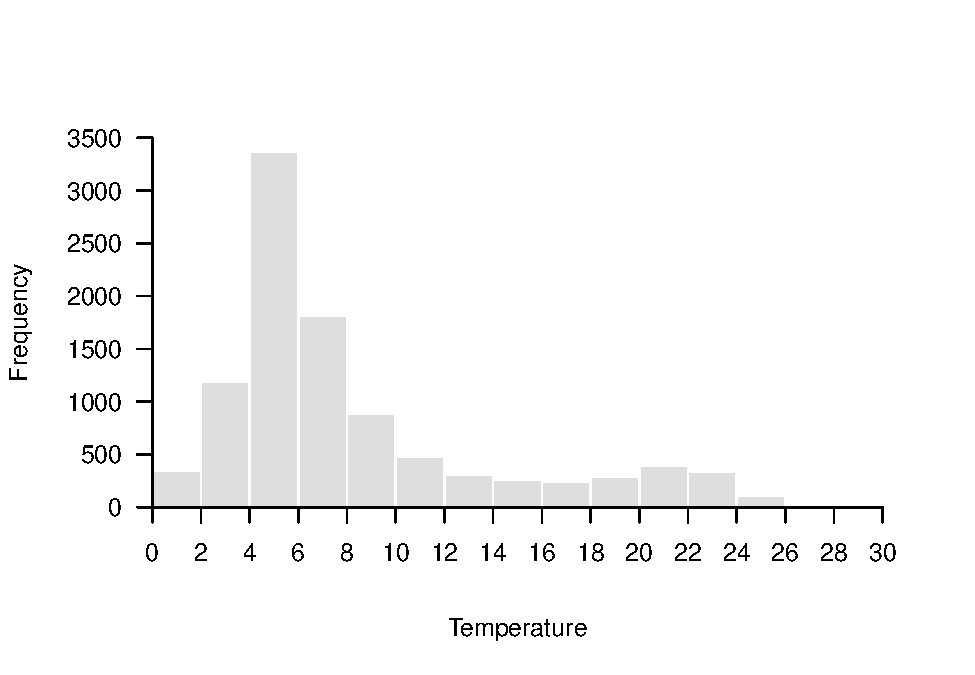
\includegraphics{worstr_files/figure-latex/unnamed-chunk-88-1.pdf}

\textbf{Colors!!!}

If \texttt{gray87} is not your style (whatevs), there are another 656 pre-named colors in R. You can see their names by running \texttt{colors()} in the console like this:

\begin{Shaded}
\begin{Highlighting}[]
\KeywordTok{colors}\NormalTok{()}
\end{Highlighting}
\end{Shaded}

If you are a little more adventurous, you might try the \texttt{rgb()} color specification or hex values. I really like the \texttt{rgb()} specification because you can include an \texttt{alpha} channel to make your colors transparent (oooooh!). For example, if I change my code above to use the following:

\begin{Shaded}
\begin{Highlighting}[]
\NormalTok{col =}\StringTok{ }\KeywordTok{rgb}\NormalTok{(}\DataTypeTok{red =} \FloatTok{0.90}\NormalTok{, }\DataTypeTok{green =} \DecValTok{0}\NormalTok{, }\DataTypeTok{blue =} \FloatTok{0.30}\NormalTok{, }\DataTypeTok{alpha =} \FloatTok{0.10}\NormalTok{)}
\end{Highlighting}
\end{Shaded}

I get a transparent, purple histogram.

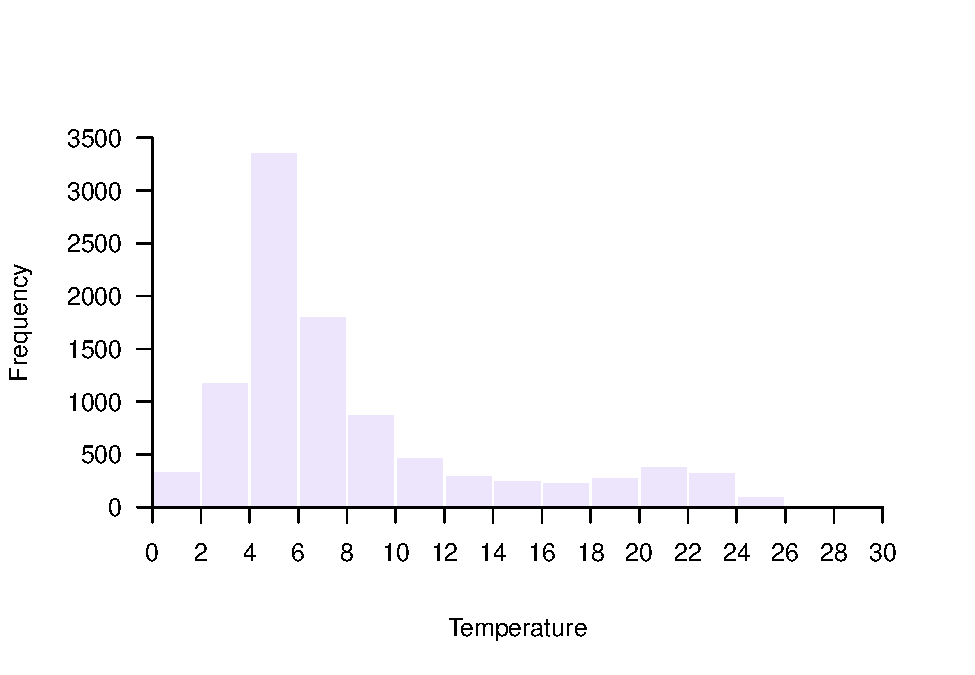
\includegraphics{worstr_files/figure-latex/unnamed-chunk-91-1.pdf}

So purply.

There are tons of great blogs and eBooks with whole chapters devoted to colors and color palletes in R. There are even whole packages we'll work with dedicated to colors. By all means, check them out! We will work with a few as we continue to increase complexity.

\hypertarget{scatterplots}{%
\subsection{Scatterplots}\label{scatterplots}}

Scatter plots are a great starting point for doing exploratory data analysis or for displaying raw data along with summary graphics. They are also the default behavior for the \texttt{plot()} function for continuous variables in base R.

Let's demonstrate by by plotting surface temperature (\texttt{depth} = 0.1 m) by month across years. We'll use the data management skills we picked up in \protect\hyperlink{Chapterux5cux25203}{Chapter 3} to filter the data first.

\begin{Shaded}
\begin{Highlighting}[]
\CommentTok{# Filter to get July surface temperatures}
\NormalTok{surface <-}\StringTok{ }\NormalTok{otsego }\OperatorTok\StringTok{ }\KeywordTok{filter}\NormalTok{(depth }\OperatorTok{==}\StringTok{ }\FloatTok{0.1}\NormalTok{)}

\CommentTok{# Default scatter plot}
\KeywordTok{plot}\NormalTok{(}\DataTypeTok{x =}\NormalTok{ surface}\OperatorTok{$}\NormalTok{month, }\DataTypeTok{y =}\NormalTok{ surface}\OperatorTok{$}\NormalTok{temp)}
\end{Highlighting}
\end{Shaded}

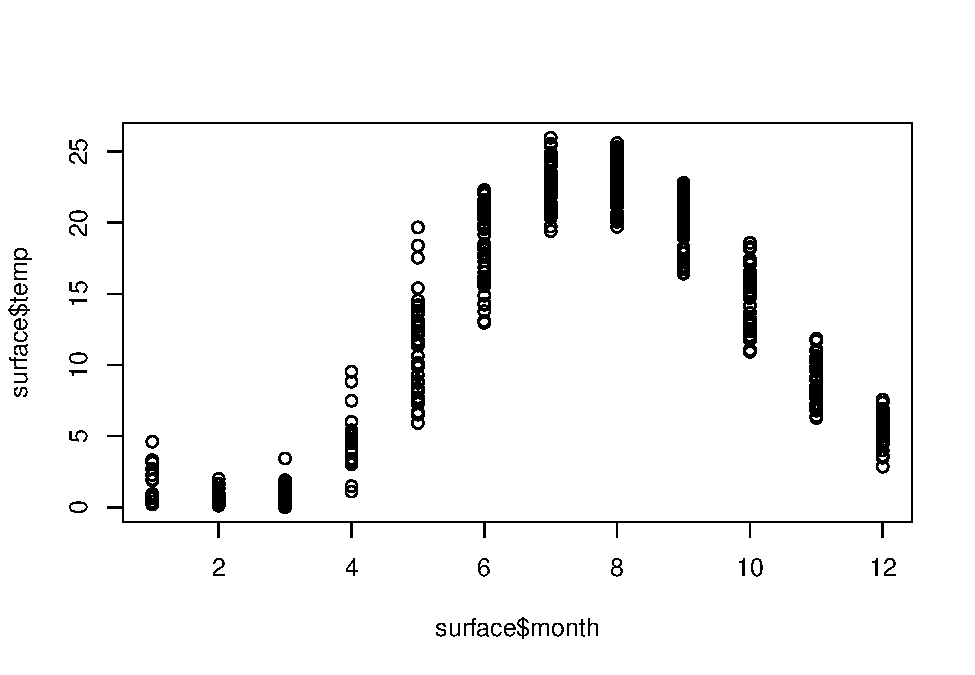
\includegraphics{worstr_files/figure-latex/unnamed-chunk-92-1.pdf}

As with the \texttt{hist()} function, the default here is underwhelming. We can use many of the same arguments that we specified in \texttt{hist()} to dress this up a bit. This time, we will specify a plotting character \texttt{pch} that corresponds to a filled circle. Then, we tell R to give it an \texttt{rgb()} background (\texttt{bg}) with no color for lines that go around each point. That way the data points are darker where there is overlap between them. Finally, we use \texttt{expression()} to include the degree symbol in the y-axis label.

\begin{Shaded}
\begin{Highlighting}[]
\CommentTok{# Better scatter plot}
\KeywordTok{plot}\NormalTok{(}\DataTypeTok{x =}\NormalTok{ surface}\OperatorTok{$}\NormalTok{month, }
     \DataTypeTok{y =}\NormalTok{ surface}\OperatorTok{$}\NormalTok{temp,}
     \DataTypeTok{pch =} \DecValTok{21}\NormalTok{,}
     \DataTypeTok{bg =} \KeywordTok{rgb}\NormalTok{(}\DecValTok{0}\NormalTok{, }\DecValTok{0}\NormalTok{, }\DecValTok{0}\NormalTok{, }\FloatTok{0.2}\NormalTok{),}
     \DataTypeTok{col =} \OtherTok{NA}\NormalTok{,}
     \DataTypeTok{xlab =} \StringTok{"Month"}\NormalTok{,}
     \DataTypeTok{ylab =} \KeywordTok{expression}\NormalTok{(}\KeywordTok{paste}\NormalTok{(}\StringTok{"Temperature ( "}\NormalTok{, degree, }\StringTok{"C)"}\NormalTok{))}
\NormalTok{     )}
\end{Highlighting}
\end{Shaded}

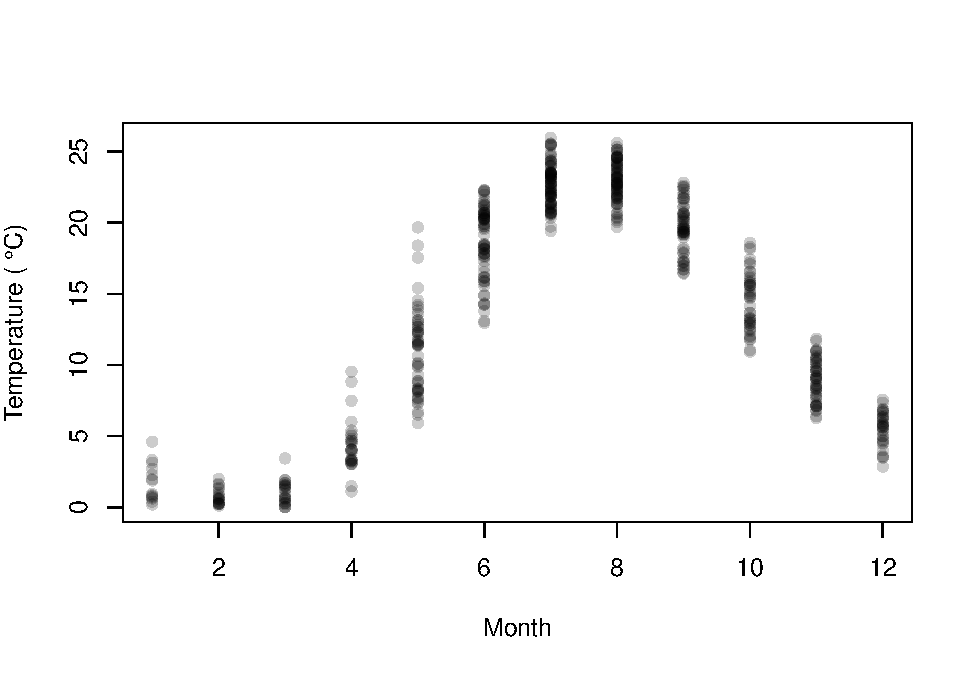
\includegraphics{worstr_files/figure-latex/unnamed-chunk-93-1.pdf}

This is a lot more informative because it shows us where most of the observations fall within a given month, and how much variability there is. But, it would be nice to have some summary.

\hypertarget{lines}{%
\subsection{Lines}\label{lines}}

We can plot lines in a few different ways in the base graphics of R. We can create stand-alone line graphs with data in R pretty easily with the \texttt{plot()} function we used for scatter plots in the preceding section.

For example, let's say that we want to just plot average surface temperature in each month as a line graph. We can summarize the data quickly and then plot those:

\begin{Shaded}
\begin{Highlighting}[]
\NormalTok{mids <-}\StringTok{ }\NormalTok{surface }\OperatorTok
\StringTok{  }\KeywordTok{group_by}\NormalTok{(month) }\OperatorTok
\StringTok{  }\KeywordTok{summarize}\NormalTok{(}\DataTypeTok{avg =} \KeywordTok{mean}\NormalTok{(temp))}

\KeywordTok{plot}\NormalTok{(mids}\OperatorTok{$}\NormalTok{month, mids}\OperatorTok{$}\NormalTok{avg, }\DataTypeTok{type =} \StringTok{"l"}\NormalTok{, }\DataTypeTok{xlab =} \StringTok{"Month"}\NormalTok{, }\DataTypeTok{ylab =} \StringTok{"Average"}\NormalTok{)}
\end{Highlighting}
\end{Shaded}

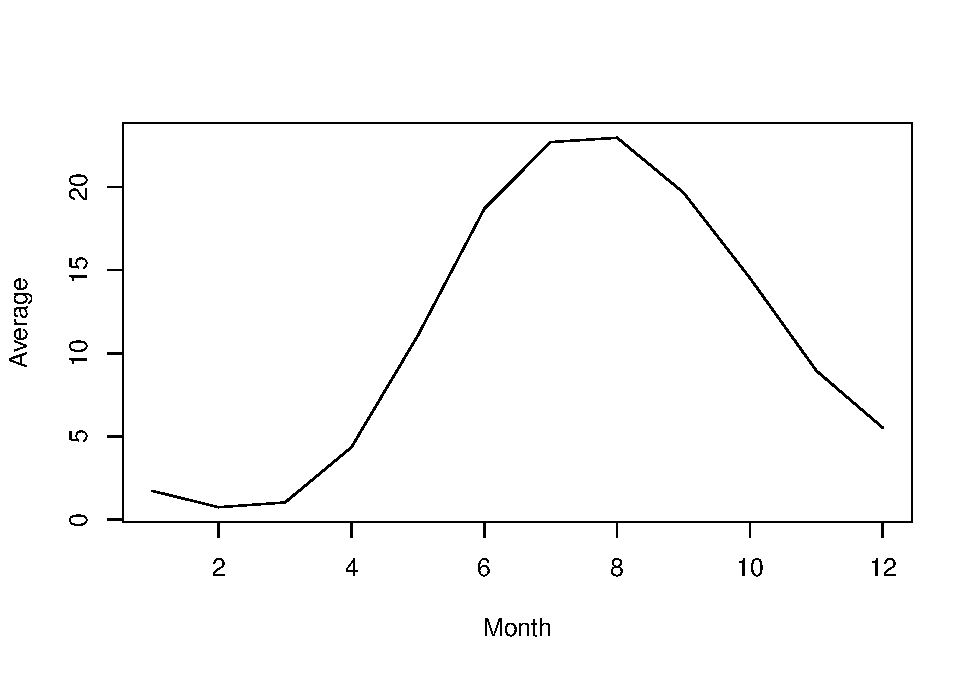
\includegraphics{worstr_files/figure-latex/unnamed-chunk-94-1.pdf}

We could even add these to the scatter plot of our raw data using the \texttt{lines()} function. Play around with \texttt{lty} and \texttt{lwd} to see if you can figure out what they do. If you get stuck, don't forget to Google it! (Worst Stats Text eveR.)

\begin{Shaded}
\begin{Highlighting}[]
\CommentTok{# Same scatter plot}
\KeywordTok{plot}\NormalTok{(}\DataTypeTok{x =}\NormalTok{ surface}\OperatorTok{$}\NormalTok{month, }
     \DataTypeTok{y =}\NormalTok{ surface}\OperatorTok{$}\NormalTok{temp,}
     \DataTypeTok{pch =} \DecValTok{21}\NormalTok{,}
     \DataTypeTok{bg =} \KeywordTok{rgb}\NormalTok{(}\DecValTok{0}\NormalTok{, }\DecValTok{0}\NormalTok{, }\DecValTok{0}\NormalTok{, }\FloatTok{0.2}\NormalTok{),}
     \DataTypeTok{col =} \OtherTok{NA}\NormalTok{,}
     \DataTypeTok{xlab =} \StringTok{"Month"}\NormalTok{,}
     \DataTypeTok{ylab =} \KeywordTok{expression}\NormalTok{(}\KeywordTok{paste}\NormalTok{(}\StringTok{"Temperature ( "}\NormalTok{, degree, }\StringTok{"C)"}\NormalTok{))}
\NormalTok{     )}
\CommentTok{# Add a thick, dotted line that is gray (this is a gray40 job)}
\KeywordTok{lines}\NormalTok{(mids}\OperatorTok{$}\NormalTok{month, mids}\OperatorTok{$}\NormalTok{avg, }\DataTypeTok{lty =} \DecValTok{3}\NormalTok{, }\DataTypeTok{lwd =} \DecValTok{2}\NormalTok{, }\DataTypeTok{col =} \StringTok{"gray40"}\NormalTok{)}
\end{Highlighting}
\end{Shaded}

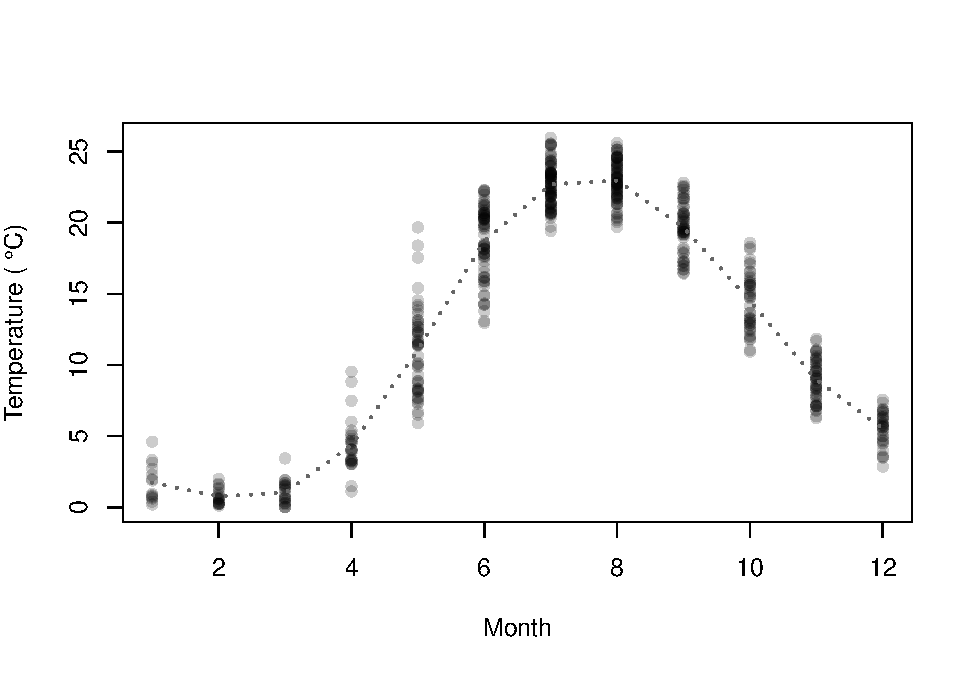
\includegraphics{worstr_files/figure-latex/unnamed-chunk-95-1.pdf}

We could also add the means to the main plot with \texttt{points()} and choose a different size or color than the raw data. We'll look at these options and more as we step up complexity.

For raw data like these, though, we are better off using a box plot to show those types of summaries.

\hypertarget{boxplots}{%
\subsection{Boxplots}\label{boxplots}}

The basic box plot is straightforward to create, but can be a real pain to modify because the syntax is slightly different from the other plotting functions we've worked with so far.

Let's try to summarize surface temperature by month using a box plot to see how these work in the base R graphics. Notice that we are specifying the variables as a formula here, and explicitly telling R what the data set is:

\begin{Shaded}
\begin{Highlighting}[]
\KeywordTok{boxplot}\NormalTok{(temp}\OperatorTok{~}\NormalTok{month, }\DataTypeTok{data =}\NormalTok{ surface,}
        \DataTypeTok{xlab =} \StringTok{"Month"}\NormalTok{,}
        \DataTypeTok{ylab =} \KeywordTok{expression}\NormalTok{(}\KeywordTok{paste}\NormalTok{(}\StringTok{"Surface temperature ( "}\NormalTok{, degree, }\StringTok{"C)"}\NormalTok{)))}
\end{Highlighting}
\end{Shaded}

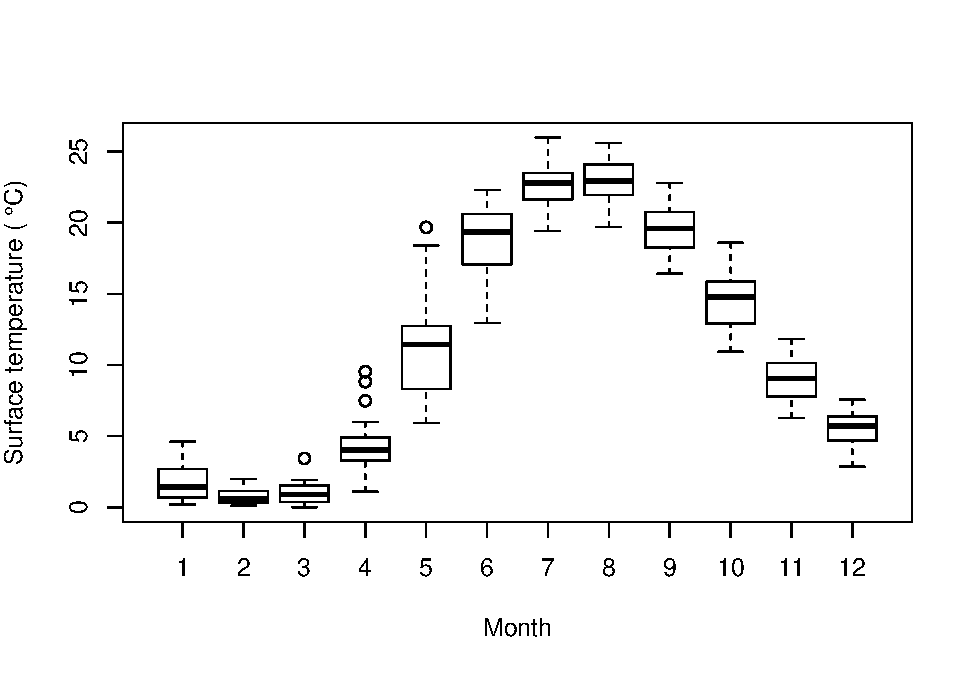
\includegraphics{worstr_files/figure-latex/unnamed-chunk-96-1.pdf}

Wow, that was waaaaay to easy! Have you ever tried to make one of those in Excel? Forget about it. It would take you half a day, and then when you realized you forgot ten data points you would have to do it all again.

But, it is still much ugly. Maybe there is a way we can change that?

Of course there is!

Let's add a little color and tweak some options. For a full set of optional arguments you can change, run \texttt{?bxp} in the console. (Ooh, that one is sneaky: \texttt{bxp()} is the function inside of \texttt{boxplot()} that actually draws the plots).

Options are named consistently by the part of the plot. For example, \texttt{boxwex}, \texttt{boxcol} and \texttt{boxfill} all control the look of the box. Likewise, the options \texttt{boxcol}, \texttt{whiskcol} and \texttt{staplecol} control the colors of the box, whiskers, and staples, respectively. Nifty, right? Play with the settings below to see what each one does. Then, go explore some more options.It is the easiest way to learn when you are learning from The Worst Stats Text eveR.

\begin{Shaded}
\begin{Highlighting}[]
\KeywordTok{boxplot}\NormalTok{(temp}\OperatorTok{~}\NormalTok{month, }
        \DataTypeTok{data =}\NormalTok{ surface,}
        \DataTypeTok{xlab =} \StringTok{"Month"}\NormalTok{,}
        \DataTypeTok{ylab =} \KeywordTok{expression}\NormalTok{(}\KeywordTok{paste}\NormalTok{(}\StringTok{"Surface temperature ( "}\NormalTok{, degree, }\StringTok{"C)"}\NormalTok{)),      }
        \DataTypeTok{border =} \StringTok{"gray40"}\NormalTok{,}
        \DataTypeTok{boxwex =} \FloatTok{0.50}\NormalTok{, }\DataTypeTok{boxcol =} \StringTok{"gray40"}\NormalTok{, }\DataTypeTok{boxfill =} \StringTok{"gray87"}\NormalTok{,}
        \DataTypeTok{whisklty =} \DecValTok{1}\NormalTok{, }\DataTypeTok{whisklwd=}\DecValTok{1}\NormalTok{, }\DataTypeTok{whiskcol =} \StringTok{"gray40"}\NormalTok{,}
        \DataTypeTok{staplewex =} \DecValTok{0}\NormalTok{, }\DataTypeTok{staplecol =} \OtherTok{NA}\NormalTok{,}
        \DataTypeTok{outpch =} \DecValTok{21}\NormalTok{, }\DataTypeTok{outbg =} \StringTok{"gray90"}\NormalTok{, }\DataTypeTok{outcol =} \StringTok{"gray90"}
\NormalTok{        )}
\end{Highlighting}
\end{Shaded}

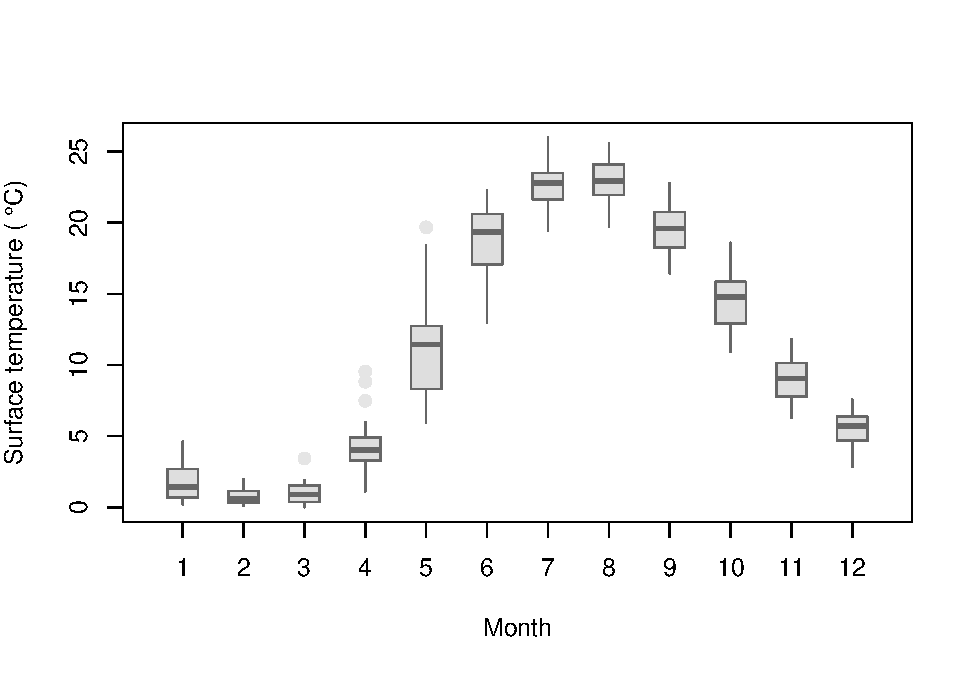
\includegraphics{worstr_files/figure-latex/unnamed-chunk-97-1.pdf}

Finally, we can combine this with a scatter plot to \texttt{jitter} our raw data over the top of the boxes in each month:

\begin{Shaded}
\begin{Highlighting}[]
\KeywordTok{boxplot}\NormalTok{(temp}\OperatorTok{~}\NormalTok{month, }
        \DataTypeTok{data =}\NormalTok{ surface,}
        \DataTypeTok{xlab =} \StringTok{"Month"}\NormalTok{,}
        \DataTypeTok{ylab =} \KeywordTok{expression}\NormalTok{(}\KeywordTok{paste}\NormalTok{(}\StringTok{"Surface temperature ( "}\NormalTok{, degree, }\StringTok{"C)"}\NormalTok{)),      }
        \DataTypeTok{border =} \StringTok{"gray40"}\NormalTok{,}
        \DataTypeTok{boxwex =} \FloatTok{0.50}\NormalTok{, }\DataTypeTok{boxcol =} \StringTok{"gray40"}\NormalTok{, }\DataTypeTok{boxfill =} \StringTok{"gray87"}\NormalTok{,}
        \DataTypeTok{whisklty =} \DecValTok{1}\NormalTok{, }\DataTypeTok{whisklwd=}\DecValTok{1}\NormalTok{, }\DataTypeTok{whiskcol =} \StringTok{"gray40"}\NormalTok{,}
        \DataTypeTok{staplewex =} \DecValTok{0}\NormalTok{, }\DataTypeTok{staplecol =} \OtherTok{NA}\NormalTok{,}
        \DataTypeTok{outpch =} \DecValTok{21}\NormalTok{, }\DataTypeTok{outbg =} \OtherTok{NA}\NormalTok{, }\DataTypeTok{outcol =} \OtherTok{NA}
\NormalTok{        )}
\KeywordTok{points}\NormalTok{(}\KeywordTok{jitter}\NormalTok{(surface}\OperatorTok{$}\NormalTok{month), surface}\OperatorTok{$}\NormalTok{temp, }\DataTypeTok{cex=}\NormalTok{.}\DecValTok{4}\NormalTok{, }\DataTypeTok{pch=}\DecValTok{19}\NormalTok{, }\DataTypeTok{col=}\KeywordTok{rgb}\NormalTok{(}\DecValTok{0}\NormalTok{,}\DecValTok{0}\NormalTok{,}\DecValTok{0}\NormalTok{,}\FloatTok{0.2}\NormalTok{))}
\end{Highlighting}
\end{Shaded}

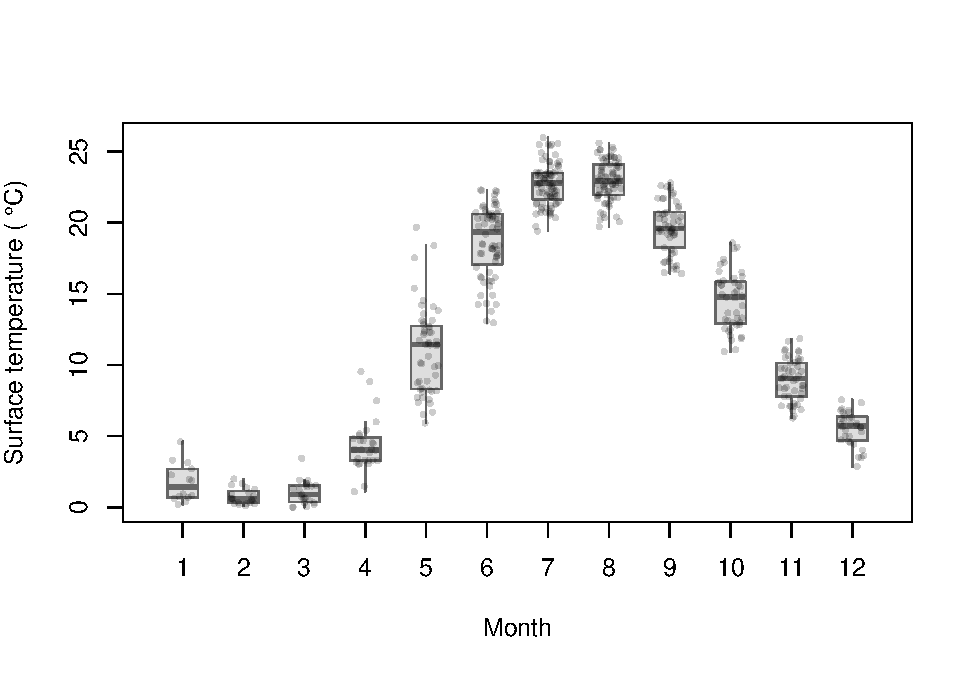
\includegraphics{worstr_files/figure-latex/unnamed-chunk-98-1.pdf}

That is actually starting to look pretty snazzy! We'll continue to work to improve our base graphics as we move forward. For now, let's have a look at how to do these things in \texttt{ggplot2} next.

\hypertarget{plotting-with-ggplot2}{%
\section{\texorpdfstring{Plotting with \texttt{ggplot2}}{Plotting with ggplot2}}\label{plotting-with-ggplot2}}

Plotting with \href{https://ggplot2.tidyverse.org/}{\texttt{ggplot2}} and the dozens of packages that use it is a bit different than plotting with base graphics in R. Part of the reason for this is that it uses a work flow that is similar to the data manipulation we have looked at so far. In general, you could think of this as creating a canvas, applying some routine aesthetics based on the data structure (e.g.~grouping), and then adding layers on to the canvas like we did with \protect\hyperlink{base-graphics}{base graphics}.

It takes a little getting used to, but you'll see how powerful it can be for multifaceted plots when we get to later chapters. We'll walk through the same plots that we did in \protect\hyperlink{base-graphics}{base graphics}, but this time we'll use the \texttt{ggplot()} function and layer on the pieces.

\hypertarget{gghists}{%
\subsection{Histograms}\label{gghists}}

The default histogram is easy to create with \texttt{ggplot()} and a geometry layer. We start with the \texttt{ggplot} call, and then add the histogram geometry, \texttt{geom\_histogram()}, like this. I usually save the plot to an object with an arbitrary name I don't use for anything, like \texttt{p} or \texttt{s} or \texttt{v}, and then print it explicitly.

\begin{Shaded}
\begin{Highlighting}[]
\CommentTok{# Histogram of water temperature across }
\CommentTok{# all dates and depths}
\NormalTok{p <-}\StringTok{ }\KeywordTok{ggplot}\NormalTok{(otsego, }\KeywordTok{aes}\NormalTok{(}\DataTypeTok{x=}\NormalTok{temp)) }\OperatorTok{+}\StringTok{ }\KeywordTok{geom_histogram}\NormalTok{(}\DataTypeTok{bins=}\DecValTok{30}\NormalTok{)}

\KeywordTok{print}\NormalTok{(p)}
\end{Highlighting}
\end{Shaded}

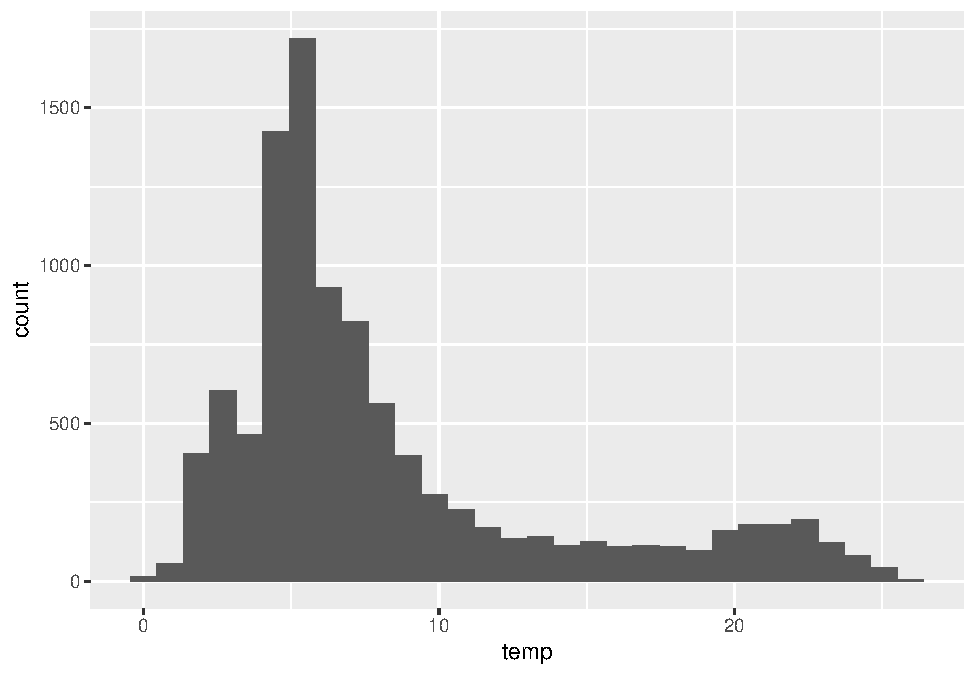
\includegraphics{worstr_files/figure-latex/unnamed-chunk-99-1.pdf}

Right away this looks a lot prettier than the default histogram that we produced with base graphics. Of course, we can customize just like we did before.

Let's add labels for the x and y-axis next:

\begin{Shaded}
\begin{Highlighting}[]
\CommentTok{# Histogram of water temperature across }
\CommentTok{# all dates and depths}
\NormalTok{p <-}\StringTok{ }\KeywordTok{ggplot}\NormalTok{(otsego, }\KeywordTok{aes}\NormalTok{(}\DataTypeTok{x=}\NormalTok{temp)) }\OperatorTok{+}\StringTok{ }
\StringTok{  }\KeywordTok{geom_histogram}\NormalTok{(}\DataTypeTok{bins=}\DecValTok{30}\NormalTok{) }\OperatorTok{+}\StringTok{ }
\StringTok{  }\KeywordTok{xlab}\NormalTok{(}\KeywordTok{expression}\NormalTok{(}\KeywordTok{paste}\NormalTok{(}\StringTok{"Temperature ("}\NormalTok{, degree, }\StringTok{"C)"}\NormalTok{))) }\OperatorTok{+}
\StringTok{  }\KeywordTok{ylab}\NormalTok{(}\StringTok{"Count"}\NormalTok{)}

\KeywordTok{print}\NormalTok{(p)}
\end{Highlighting}
\end{Shaded}

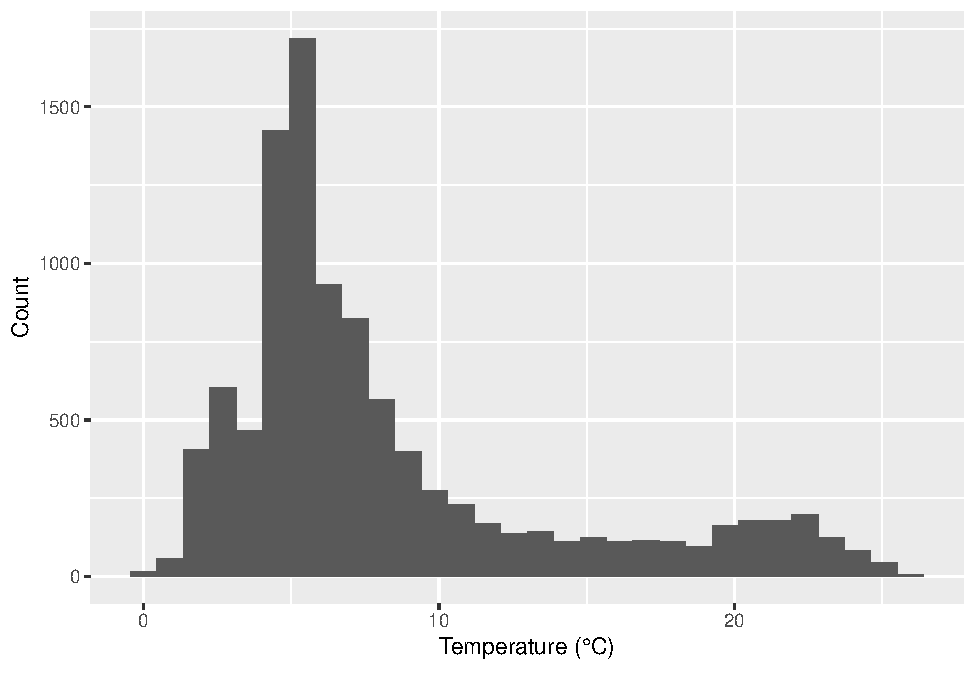
\includegraphics{worstr_files/figure-latex/unnamed-chunk-100-1.pdf}

We can also scale the \texttt{x-axis} and the \texttt{y-axis} like we did in the \protect\hyperlink{histograms}{base graphics example}.

\begin{Shaded}
\begin{Highlighting}[]
\CommentTok{# Histogram of water temperature across }
\CommentTok{# all dates and depths}
\NormalTok{p <-}\StringTok{ }\KeywordTok{ggplot}\NormalTok{(otsego, }\KeywordTok{aes}\NormalTok{(}\DataTypeTok{x=}\NormalTok{temp)) }\OperatorTok{+}\StringTok{ }
\StringTok{  }\KeywordTok{geom_histogram}\NormalTok{(}\DataTypeTok{bins=}\DecValTok{30}\NormalTok{) }\OperatorTok{+}\StringTok{ }
\StringTok{  }\KeywordTok{xlab}\NormalTok{(}\KeywordTok{expression}\NormalTok{(}\KeywordTok{paste}\NormalTok{(}\StringTok{"Temperature ("}\NormalTok{, degree, }\StringTok{"C)"}\NormalTok{))) }\OperatorTok{+}
\StringTok{  }\KeywordTok{ylab}\NormalTok{(}\StringTok{"Count"}\NormalTok{) }\OperatorTok{+}
\StringTok{  }\KeywordTok{scale_x_continuous}\NormalTok{(}\DataTypeTok{limits=}\KeywordTok{c}\NormalTok{(}\DecValTok{0}\NormalTok{, }\DecValTok{25}\NormalTok{), }\DataTypeTok{expand =} \KeywordTok{c}\NormalTok{(}\DecValTok{0}\NormalTok{, }\DecValTok{0}\NormalTok{)) }\OperatorTok{+}\StringTok{ }
\StringTok{  }\KeywordTok{scale_y_continuous}\NormalTok{(}\DataTypeTok{expand =} \KeywordTok{c}\NormalTok{(}\DecValTok{0}\NormalTok{, }\DecValTok{0}\NormalTok{))}
\KeywordTok{print}\NormalTok{(p)}
\end{Highlighting}
\end{Shaded}

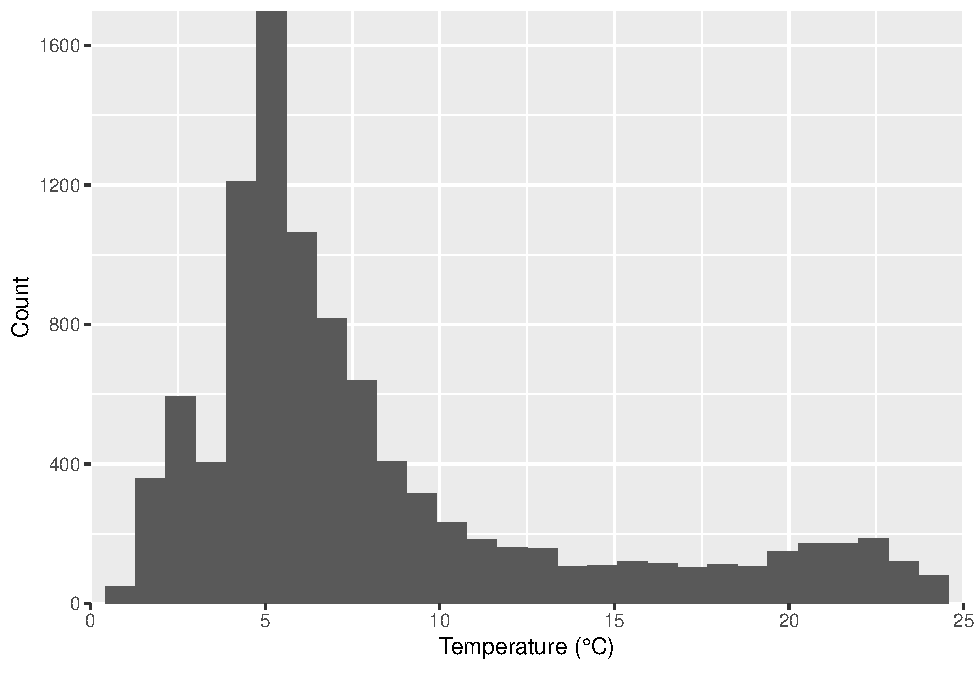
\includegraphics{worstr_files/figure-latex/unnamed-chunk-101-1.pdf}

We can modify each of other layers individually, all at once using preset ggplot \href{http://www.sthda.com/english/wiki/ggplot2-title-main-axis-and-legend-titles}{themes} or by modifying a pre-defined theme.

Let's have a look at how a theme changes the appearance. I am going to add \texttt{theme\_bw()} here, but check out the others linked above. I also add a few adjust the position of the x- and y-axis labels and removed the panel grid in the \texttt{theme()} function after applying a theme.

\begin{Shaded}
\begin{Highlighting}[]
\CommentTok{# Histogram of water temperature across }
\CommentTok{# all dates and depths}
\NormalTok{p <-}\StringTok{ }\KeywordTok{ggplot}\NormalTok{(otsego, }\KeywordTok{aes}\NormalTok{(}\DataTypeTok{x=}\NormalTok{temp)) }\OperatorTok{+}\StringTok{ }
\StringTok{  }\KeywordTok{geom_histogram}\NormalTok{(}\DataTypeTok{bins=}\DecValTok{30}\NormalTok{) }\OperatorTok{+}\StringTok{ }
\StringTok{  }\KeywordTok{scale_x_continuous}\NormalTok{(}\DataTypeTok{limits=}\KeywordTok{c}\NormalTok{(}\DecValTok{0}\NormalTok{, }\DecValTok{25}\NormalTok{), }\DataTypeTok{expand =} \KeywordTok{c}\NormalTok{(}\DecValTok{0}\NormalTok{, }\DecValTok{0}\NormalTok{)) }\OperatorTok{+}\StringTok{ }
\StringTok{  }\KeywordTok{scale_y_continuous}\NormalTok{(}\DataTypeTok{expand =} \KeywordTok{c}\NormalTok{(}\DecValTok{0}\NormalTok{, }\DecValTok{0}\NormalTok{)) }\OperatorTok{+}\StringTok{ }
\StringTok{  }\KeywordTok{xlab}\NormalTok{(}\KeywordTok{expression}\NormalTok{(}\KeywordTok{paste}\NormalTok{(}\StringTok{"Temperature ("}\NormalTok{, degree, }\StringTok{"C)"}\NormalTok{))) }\OperatorTok{+}
\StringTok{  }\KeywordTok{ylab}\NormalTok{(}\StringTok{"Count"}\NormalTok{) }\OperatorTok{+}
\StringTok{  }\KeywordTok{theme_bw}\NormalTok{() }\OperatorTok{+}
\StringTok{  }\KeywordTok{theme}\NormalTok{(}
    \DataTypeTok{axis.title.x =} \KeywordTok{element_text}\NormalTok{(}\DataTypeTok{vjust =} \DecValTok{-1}\NormalTok{),}
    \DataTypeTok{axis.title.y =} \KeywordTok{element_text}\NormalTok{(}\DataTypeTok{vjust =} \DecValTok{3}\NormalTok{),}
    \DataTypeTok{panel.grid =} \KeywordTok{element_blank}\NormalTok{()}
\NormalTok{  )}
\KeywordTok{print}\NormalTok{(p)}
\end{Highlighting}
\end{Shaded}

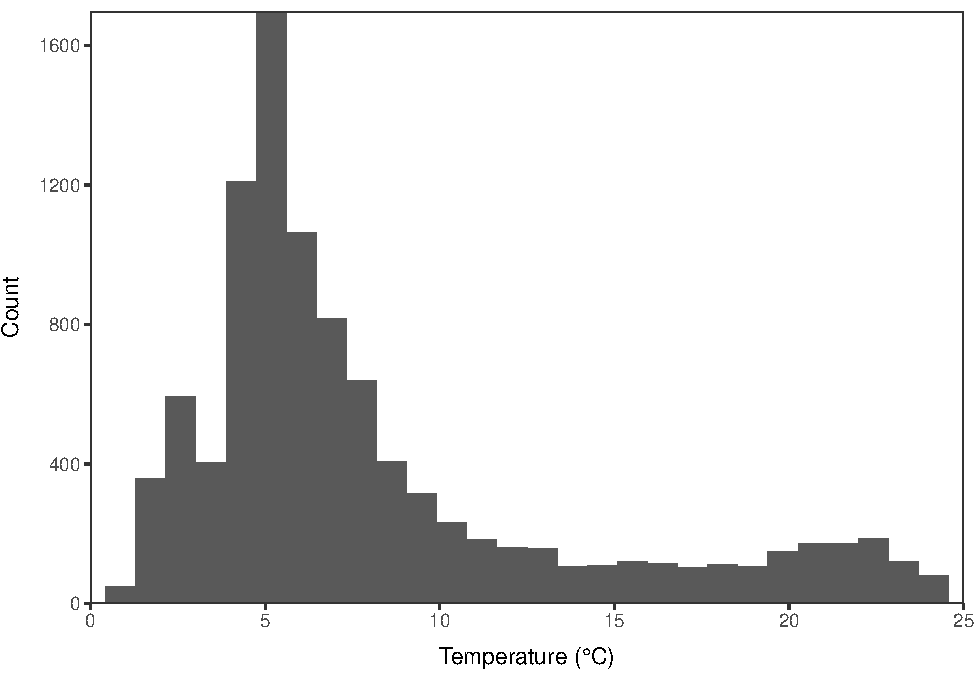
\includegraphics{worstr_files/figure-latex/unnamed-chunk-102-1.pdf}

Spend some time practicing this and changing options to see what you can come up with. Be sure to check out the descriptions of the options you can pass to theme by running \texttt{?theme} to get the help file.

\hypertarget{ggscatter}{%
\subsection{Scatter plots}\label{ggscatter}}

Now that we have a basic feel for the \texttt{ggplot2} work flow, changing plot types is really easy because all of the parts of our plots work together in the same way.

As a reminder, we previously built scatter plots of surface temperature in Otsego Lake, NY by month using base graphics.

Go ahead and subset the data again:

\begin{Shaded}
\begin{Highlighting}[]
\NormalTok{surface <-}\StringTok{ }\NormalTok{otsego }\OperatorTok\StringTok{ }\KeywordTok{filter}\NormalTok{(depth }\OperatorTok{==}\StringTok{ }\FloatTok{0.10}\NormalTok{)}
\end{Highlighting}
\end{Shaded}

Now, we can make the default scatterplot:

\begin{Shaded}
\begin{Highlighting}[]
\NormalTok{s <-}\StringTok{ }\KeywordTok{ggplot}\NormalTok{(surface, }\KeywordTok{aes}\NormalTok{(}\DataTypeTok{x =}\NormalTok{ month, }\DataTypeTok{y =}\NormalTok{ temp)) }\OperatorTok{+}
\StringTok{  }\KeywordTok{geom_point}\NormalTok{()}
\KeywordTok{print}\NormalTok{(s)}
\end{Highlighting}
\end{Shaded}

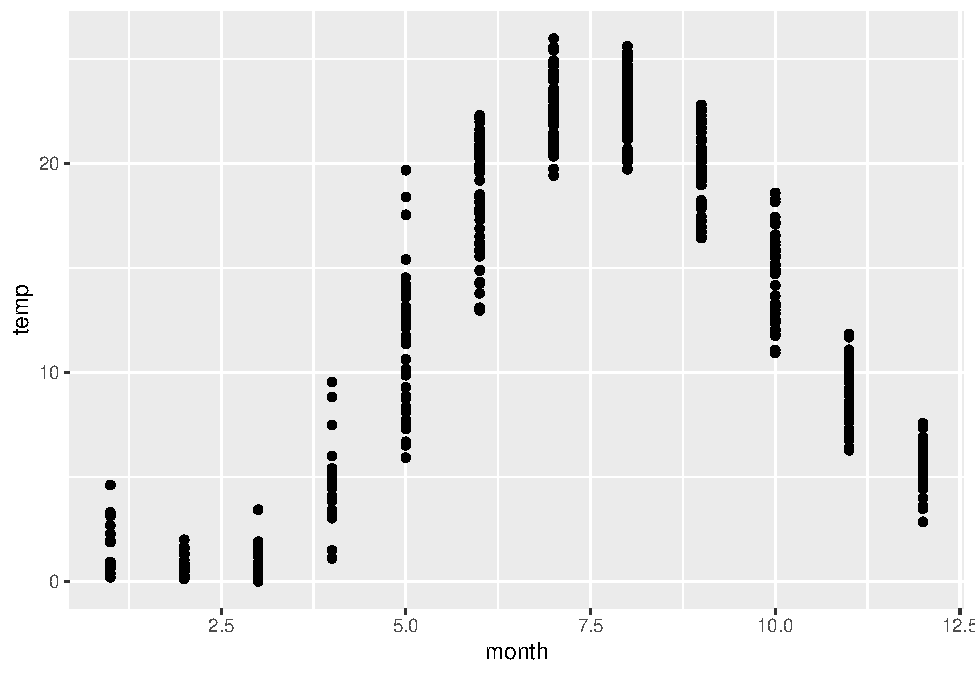
\includegraphics{worstr_files/figure-latex/unnamed-chunk-104-1.pdf}

At a glance, this already looks a lot nicer than the default scatterplots from base graphics, but we still have a lot of work to do. Plus, we get ggplots own odd behaviors when it comes to the x-axis scale and titles. So, let's get to work!

First, we'll replace the default axis titles and add the \texttt{theme\_bw()} that we used above, with the same modifications to axis positions and grid lines.

\begin{Shaded}
\begin{Highlighting}[]
\NormalTok{s <-}\StringTok{ }\KeywordTok{ggplot}\NormalTok{(surface, }\KeywordTok{aes}\NormalTok{(}\DataTypeTok{x =}\NormalTok{ month, }\DataTypeTok{y =}\NormalTok{ temp)) }\OperatorTok{+}
\StringTok{  }\KeywordTok{geom_point}\NormalTok{() }\OperatorTok{+}\StringTok{ }
\StringTok{  }\KeywordTok{xlab}\NormalTok{(}\StringTok{"Month"}\NormalTok{) }\OperatorTok{+}
\StringTok{  }\KeywordTok{ylab}\NormalTok{(}\KeywordTok{expression}\NormalTok{(}\KeywordTok{paste}\NormalTok{(}\StringTok{"Temperature ( "}\NormalTok{, degree, }\StringTok{"C)"}\NormalTok{))) }\OperatorTok{+}
\StringTok{  }\KeywordTok{theme_bw}\NormalTok{() }\OperatorTok{+}
\StringTok{  }\KeywordTok{theme}\NormalTok{(}\DataTypeTok{axis.title.x =} \KeywordTok{element_text}\NormalTok{(}\DataTypeTok{vjust =} \DecValTok{-1}\NormalTok{),}
        \DataTypeTok{axis.title.y =} \KeywordTok{element_text}\NormalTok{(}\DataTypeTok{vjust =} \DecValTok{3}\NormalTok{),}
        \DataTypeTok{panel.grid =} \KeywordTok{element_blank}\NormalTok{()}
\NormalTok{  )}
\KeywordTok{print}\NormalTok{(s)}
\end{Highlighting}
\end{Shaded}

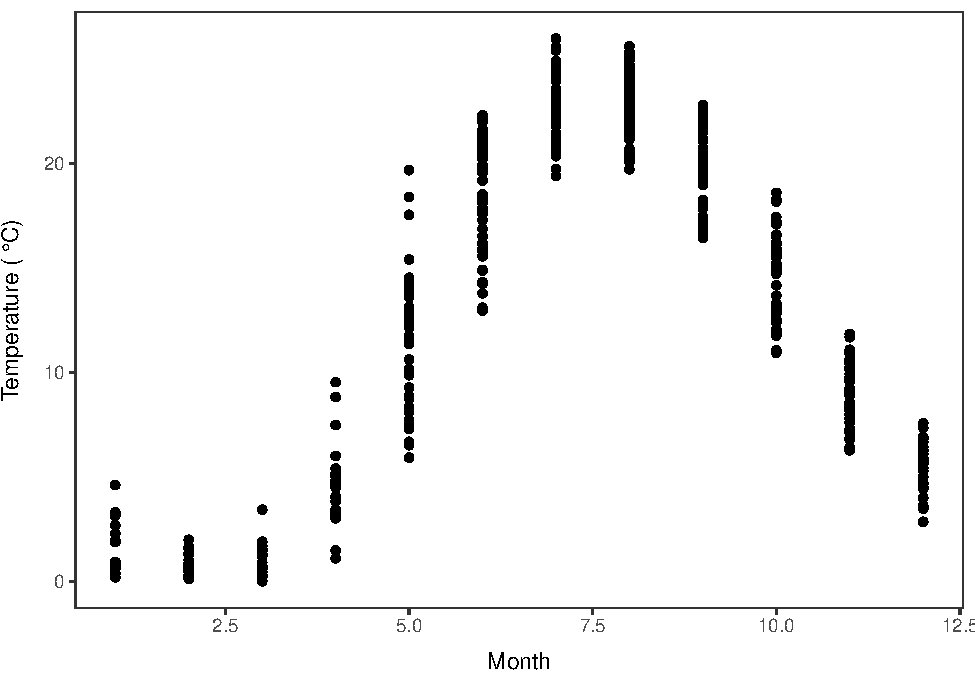
\includegraphics{worstr_files/figure-latex/unnamed-chunk-105-1.pdf}

Okay, now we need to fix that pesky x-axis scale to use whole months or text labels.

To fix the axis scales, we've actually got to do a little bit of work this time. In this case the easiest thing to do is probably to make a categorical variable out of the column \texttt{month}, which is an integer. We can do this using some fancy indexing with the built-in object that contains month abbreviations, \texttt{month.abb} in base R.

\begin{Shaded}
\begin{Highlighting}[]
\NormalTok{surface}\OperatorTok{$}\NormalTok{c_month <-}\StringTok{ }\KeywordTok{factor}\NormalTok{(month.abb[surface}\OperatorTok{$}\NormalTok{month], }\DataTypeTok{levels=}\NormalTok{month.abb)}
\end{Highlighting}
\end{Shaded}

Whoa, that was a heavy lift (sarcasm). Let's see how that changes the appearance of our plot:

\begin{Shaded}
\begin{Highlighting}[]
\NormalTok{s <-}\StringTok{ }\KeywordTok{ggplot}\NormalTok{(surface, }\KeywordTok{aes}\NormalTok{(}\DataTypeTok{x =}\NormalTok{ c_month, }\DataTypeTok{y =}\NormalTok{ temp)) }\OperatorTok{+}
\StringTok{  }\KeywordTok{geom_point}\NormalTok{() }\OperatorTok{+}\StringTok{ }
\StringTok{  }\KeywordTok{xlab}\NormalTok{(}\StringTok{"Month"}\NormalTok{) }\OperatorTok{+}
\StringTok{  }\KeywordTok{ylab}\NormalTok{(}\KeywordTok{expression}\NormalTok{(}\KeywordTok{paste}\NormalTok{(}\StringTok{"Temperature ( "}\NormalTok{, degree, }\StringTok{"C)"}\NormalTok{))) }\OperatorTok{+}
\StringTok{  }\KeywordTok{theme_bw}\NormalTok{() }\OperatorTok{+}
\StringTok{  }\KeywordTok{theme}\NormalTok{(}\DataTypeTok{axis.title.x =} \KeywordTok{element_text}\NormalTok{(}\DataTypeTok{vjust =} \DecValTok{-1}\NormalTok{),}
        \DataTypeTok{axis.title.y =} \KeywordTok{element_text}\NormalTok{(}\DataTypeTok{vjust =} \DecValTok{3}\NormalTok{),}
        \DataTypeTok{panel.grid =} \KeywordTok{element_blank}\NormalTok{()}
\NormalTok{  )}
\KeywordTok{print}\NormalTok{(s)}
\end{Highlighting}
\end{Shaded}

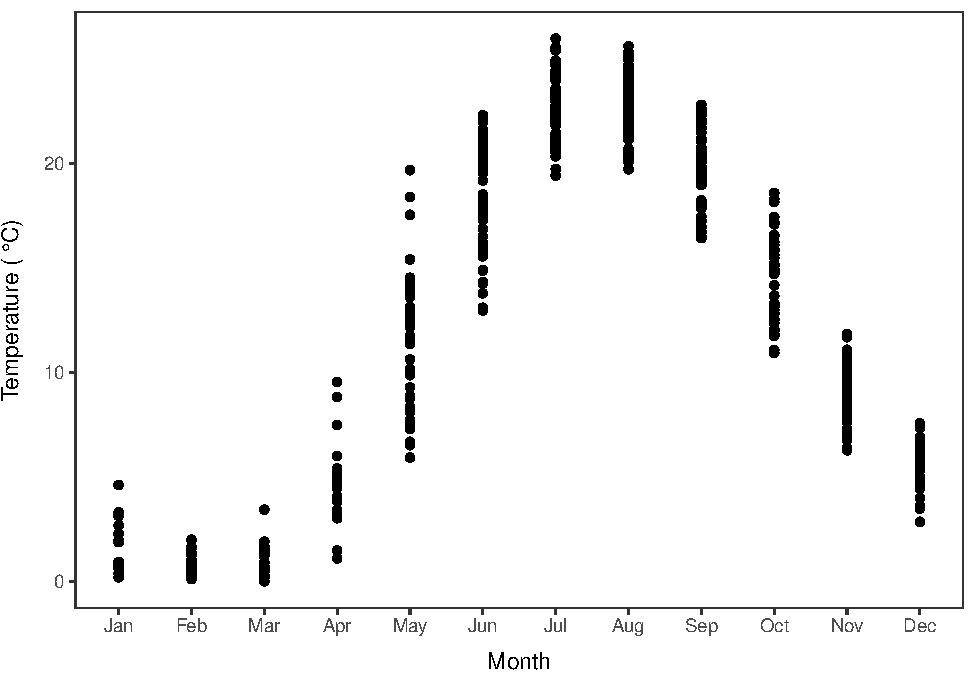
\includegraphics{worstr_files/figure-latex/unnamed-chunk-107-1.pdf}
This is starting to look really nice.

Finally, we just add a little transparency to the points by specifying \texttt{alpha\ =\ 0.2} inside of \texttt{geom\_point()} and we are good to go!

\begin{Shaded}
\begin{Highlighting}[]
\NormalTok{s <-}\StringTok{ }\KeywordTok{ggplot}\NormalTok{(surface, }\KeywordTok{aes}\NormalTok{(}\DataTypeTok{x =}\NormalTok{ c_month, }\DataTypeTok{y =}\NormalTok{ temp)) }\OperatorTok{+}
\StringTok{  }\KeywordTok{geom_point}\NormalTok{(}\DataTypeTok{alpha =} \FloatTok{0.2}\NormalTok{) }\OperatorTok{+}\StringTok{ }
\StringTok{  }\KeywordTok{xlab}\NormalTok{(}\StringTok{"Month"}\NormalTok{) }\OperatorTok{+}
\StringTok{  }\KeywordTok{ylab}\NormalTok{(}\KeywordTok{expression}\NormalTok{(}\KeywordTok{paste}\NormalTok{(}\StringTok{"Temperature ( "}\NormalTok{, degree, }\StringTok{"C)"}\NormalTok{))) }\OperatorTok{+}
\StringTok{  }\KeywordTok{theme_bw}\NormalTok{() }\OperatorTok{+}
\StringTok{  }\KeywordTok{theme}\NormalTok{(}\DataTypeTok{axis.title.x =} \KeywordTok{element_text}\NormalTok{(}\DataTypeTok{vjust =} \DecValTok{-1}\NormalTok{),}
        \DataTypeTok{axis.title.y =} \KeywordTok{element_text}\NormalTok{(}\DataTypeTok{vjust =} \DecValTok{3}\NormalTok{),}
        \DataTypeTok{panel.grid =} \KeywordTok{element_blank}\NormalTok{()}
\NormalTok{  )}
\KeywordTok{print}\NormalTok{(s)}
\end{Highlighting}
\end{Shaded}

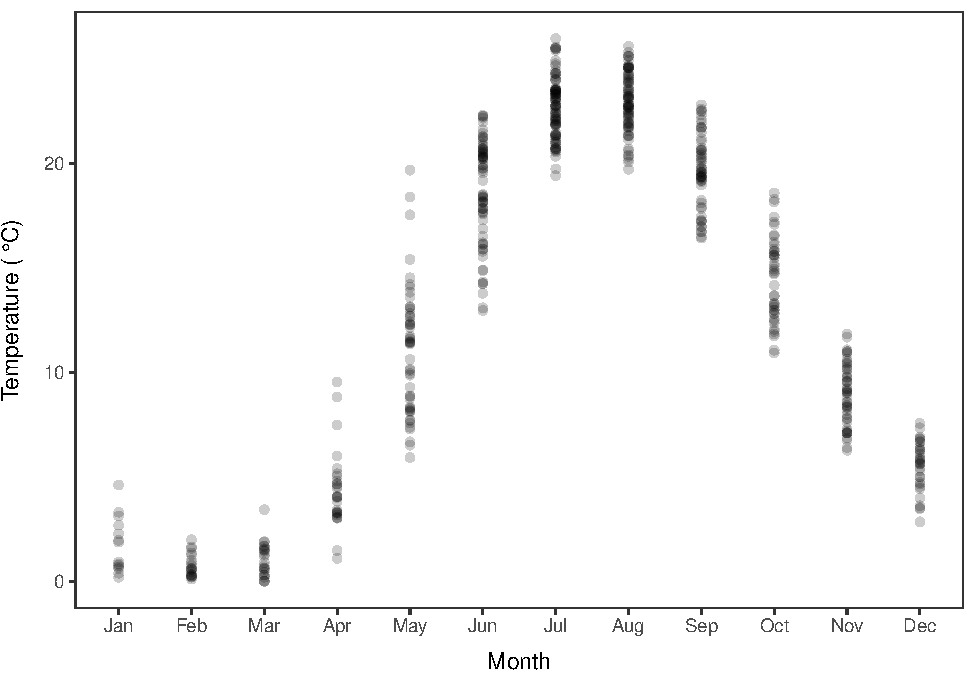
\includegraphics{worstr_files/figure-latex/unnamed-chunk-108-1.pdf}

Looks just like the one we made with base graphics!

\hypertarget{gglines}{%
\subsection{Lines}\label{gglines}}

Most of the time we plot line graphs, whether in base graphics or using \texttt{ggplot2}, we are going to be adding them to existing plots. This was really straightforward in base graphics. It is only slightly more complicated in \texttt{ggplot2}.

We'll start with the default line graph, and then add it to the scatter plot from the previous section.

Let's calculate monthly means of surface temperature in Otsego Lake again:

\begin{Shaded}
\begin{Highlighting}[]
\NormalTok{mids <-}\StringTok{ }\NormalTok{surface }\OperatorTok
\StringTok{  }\KeywordTok{group_by}\NormalTok{(month) }\OperatorTok
\StringTok{  }\KeywordTok{summarize}\NormalTok{(}\DataTypeTok{avg =} \KeywordTok{mean}\NormalTok{(temp))}
\end{Highlighting}
\end{Shaded}

Now plot it with \texttt{ggplot()}:

\begin{Shaded}
\begin{Highlighting}[]
\NormalTok{lp <-}\StringTok{ }\KeywordTok{ggplot}\NormalTok{(mids, }\KeywordTok{aes}\NormalTok{(}\DataTypeTok{x =}\NormalTok{ month, }\DataTypeTok{y =}\NormalTok{ avg)) }\OperatorTok{+}
\StringTok{  }\KeywordTok{geom_line}\NormalTok{()}

\KeywordTok{print}\NormalTok{(lp)}
\end{Highlighting}
\end{Shaded}

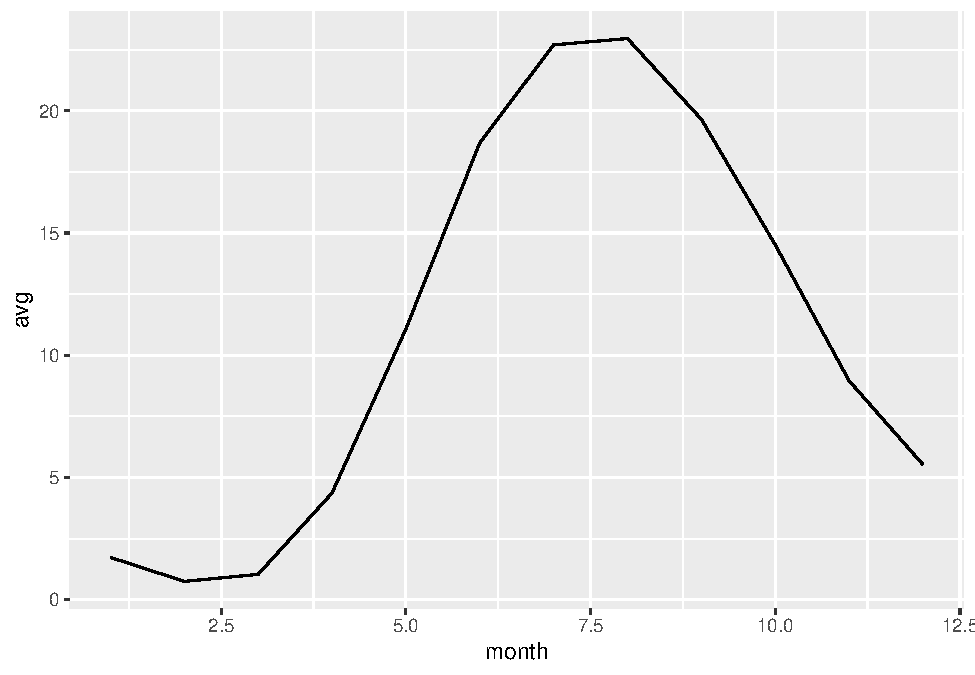
\includegraphics{worstr_files/figure-latex/unnamed-chunk-110-1.pdf}

There you have it!

Now, we just need to add this to our scatterplot that we made previously. To do this, we have to insert \texttt{geom\_line()} in the code, but we must specify

\begin{Shaded}
\begin{Highlighting}[]
\NormalTok{s <-}\StringTok{ }\KeywordTok{ggplot}\NormalTok{(}\DataTypeTok{data =}\NormalTok{ surface, }\DataTypeTok{mapping =} \KeywordTok{aes}\NormalTok{(}\DataTypeTok{x =}\NormalTok{ c_month, }\DataTypeTok{y =}\NormalTok{ temp)) }\OperatorTok{+}
\StringTok{  }\KeywordTok{geom_point}\NormalTok{(}\DataTypeTok{alpha =} \FloatTok{0.20}\NormalTok{) }\OperatorTok{+}\StringTok{ }
\StringTok{  }\KeywordTok{geom_line}\NormalTok{(}\DataTypeTok{mapping =} \KeywordTok{aes}\NormalTok{(}\DataTypeTok{x =}\NormalTok{ month, }\DataTypeTok{y =}\NormalTok{ avg),}
            \DataTypeTok{data =}\NormalTok{ mids,}
            \DataTypeTok{color =} \StringTok{'gray40'}\NormalTok{,}
            \DataTypeTok{lty =} \DecValTok{3}\NormalTok{,}
            \DataTypeTok{lwd =} \DecValTok{1}\NormalTok{) }\OperatorTok{+}
\StringTok{  }\KeywordTok{xlab}\NormalTok{(}\StringTok{"Month"}\NormalTok{) }\OperatorTok{+}
\StringTok{  }\KeywordTok{ylab}\NormalTok{(}\KeywordTok{expression}\NormalTok{(}\KeywordTok{paste}\NormalTok{(}\StringTok{"Temperature ( "}\NormalTok{, degree, }\StringTok{"C)"}\NormalTok{))) }\OperatorTok{+}
\StringTok{  }\KeywordTok{theme_bw}\NormalTok{() }\OperatorTok{+}
\StringTok{  }\KeywordTok{theme}\NormalTok{(}\DataTypeTok{axis.title.x =} \KeywordTok{element_text}\NormalTok{(}\DataTypeTok{vjust =} \DecValTok{-1}\NormalTok{),}
        \DataTypeTok{axis.title.y =} \KeywordTok{element_text}\NormalTok{(}\DataTypeTok{vjust =} \DecValTok{3}\NormalTok{),}
        \DataTypeTok{panel.grid =} \KeywordTok{element_blank}\NormalTok{()}
\NormalTok{  )}

\KeywordTok{print}\NormalTok{(s)}
\end{Highlighting}
\end{Shaded}

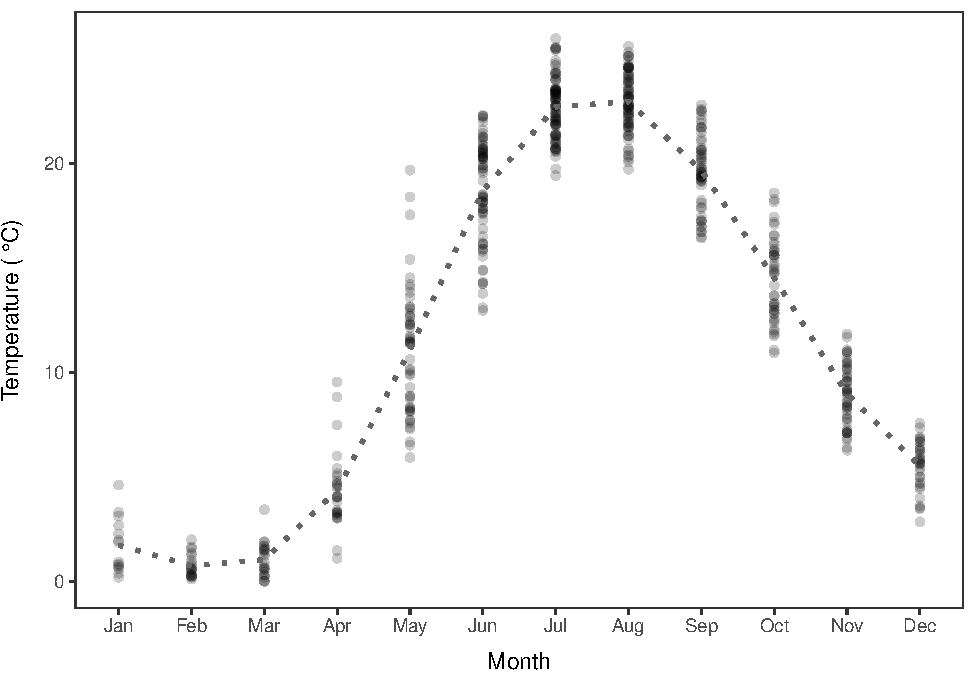
\includegraphics{worstr_files/figure-latex/unnamed-chunk-111-1.pdf}

We will continue to use this approach throughout the book to plot raw data and model predictions. So, if it is giving you trouble now, spend some extra time with it.

\hypertarget{ggboxplots}{%
\subsection{Boxplots and}\label{ggboxplots}}

To wrap up our tour of plotting examples in \texttt{ggplot2}, we will reproduce (more or less) the box plots we made in \protect\hyperlink{boxplots}{base graphics}.

Make the default box plot of surface water temperatures in Otsego Lake, NY. Notice that we use the \texttt{c\_month} variable that we made previously in the \texttt{surface} data so R knows these are groups.

\begin{Shaded}
\begin{Highlighting}[]
\NormalTok{bp <-}\StringTok{ }\KeywordTok{ggplot}\NormalTok{(surface, }\KeywordTok{aes}\NormalTok{(}\DataTypeTok{x =}\NormalTok{ c_month, }\DataTypeTok{y =}\NormalTok{ temp)) }\OperatorTok{+}\StringTok{ }\KeywordTok{geom_boxplot}\NormalTok{()}

\KeywordTok{print}\NormalTok{(bp)}
\end{Highlighting}
\end{Shaded}

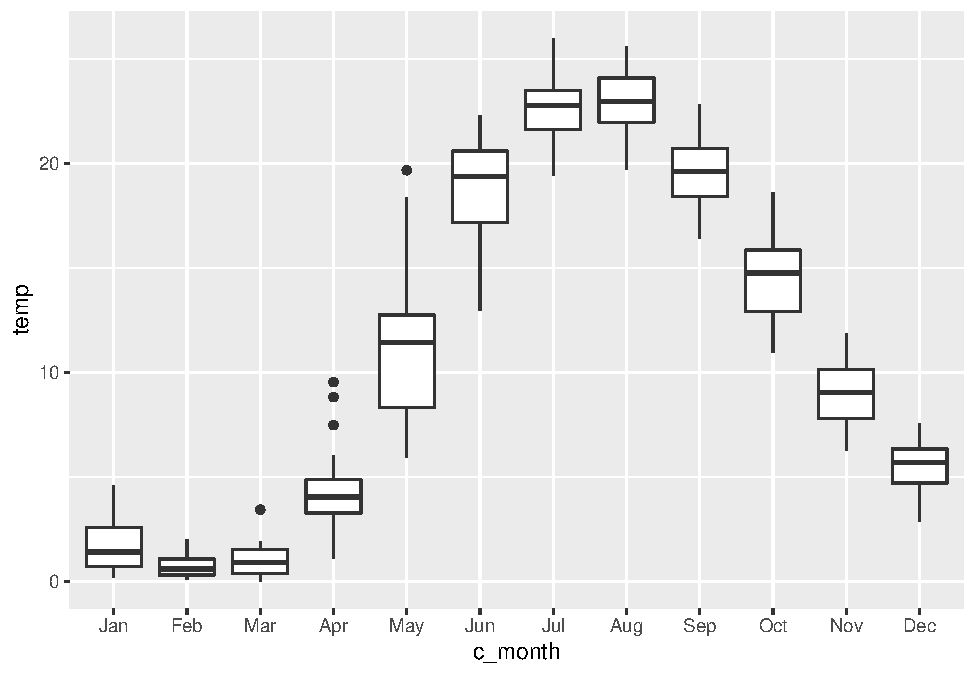
\includegraphics{worstr_files/figure-latex/unnamed-chunk-112-1.pdf}

If we add changes we made to previous plots here, then we can get a cleaner look:

\begin{Shaded}
\begin{Highlighting}[]
\NormalTok{bp <-}\StringTok{ }\KeywordTok{ggplot}\NormalTok{(surface, }\KeywordTok{aes}\NormalTok{(}\DataTypeTok{x =}\NormalTok{ c_month, }\DataTypeTok{y =}\NormalTok{ temp)) }\OperatorTok{+}
\StringTok{  }\KeywordTok{geom_boxplot}\NormalTok{(}\DataTypeTok{color =} \StringTok{'gray40'}\NormalTok{, }\DataTypeTok{fill =} \StringTok{'gray87'}\NormalTok{, }\DataTypeTok{width =} \FloatTok{0.3}\NormalTok{) }\OperatorTok{+}
\StringTok{  }\KeywordTok{xlab}\NormalTok{(}\StringTok{"Month"}\NormalTok{) }\OperatorTok{+}
\StringTok{  }\KeywordTok{ylab}\NormalTok{(}\KeywordTok{expression}\NormalTok{(}\KeywordTok{paste}\NormalTok{(}\StringTok{"Temperature ( "}\NormalTok{, degree, }\StringTok{"C)"}\NormalTok{))) }\OperatorTok{+}
\StringTok{  }\KeywordTok{theme_bw}\NormalTok{() }\OperatorTok{+}
\StringTok{  }\KeywordTok{theme}\NormalTok{(}\DataTypeTok{axis.title.x =} \KeywordTok{element_text}\NormalTok{(}\DataTypeTok{vjust =} \DecValTok{-1}\NormalTok{),}
        \DataTypeTok{axis.title.y =} \KeywordTok{element_text}\NormalTok{(}\DataTypeTok{vjust =} \DecValTok{3}\NormalTok{),}
        \DataTypeTok{panel.grid =} \KeywordTok{element_blank}\NormalTok{()}
\NormalTok{  )}

\KeywordTok{print}\NormalTok{(bp)}
\end{Highlighting}
\end{Shaded}

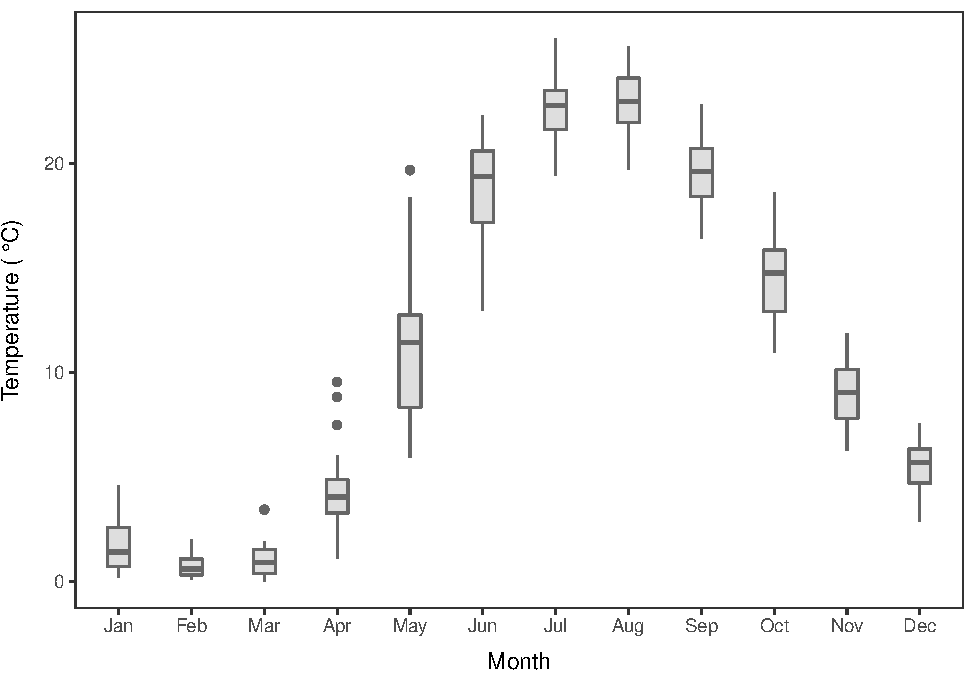
\includegraphics{worstr_files/figure-latex/unnamed-chunk-113-1.pdf}

And, of course, we can add our ``jittered'', raw data points over the top to show the spread.

\begin{Shaded}
\begin{Highlighting}[]
\NormalTok{bp <-}\StringTok{ }\KeywordTok{ggplot}\NormalTok{(surface, }\KeywordTok{aes}\NormalTok{(}\DataTypeTok{x =}\NormalTok{ c_month, }\DataTypeTok{y =}\NormalTok{ temp)) }\OperatorTok{+}
\StringTok{  }\KeywordTok{geom_boxplot}\NormalTok{(}\DataTypeTok{color =} \StringTok{'gray40'}\NormalTok{, }\DataTypeTok{fill =} \StringTok{'gray87'}\NormalTok{, }\DataTypeTok{width =} \FloatTok{0.4}\NormalTok{) }\OperatorTok{+}
\StringTok{  }\KeywordTok{geom_jitter}\NormalTok{(}\DataTypeTok{size =} \FloatTok{.5}\NormalTok{, }\DataTypeTok{width =} \FloatTok{0.1}\NormalTok{) }\OperatorTok{+}
\StringTok{  }\KeywordTok{xlab}\NormalTok{(}\StringTok{"Month"}\NormalTok{) }\OperatorTok{+}
\StringTok{  }\KeywordTok{ylab}\NormalTok{(}\KeywordTok{expression}\NormalTok{(}\KeywordTok{paste}\NormalTok{(}\StringTok{"Temperature ( "}\NormalTok{, degree, }\StringTok{"C)"}\NormalTok{))) }\OperatorTok{+}
\StringTok{  }\KeywordTok{theme_bw}\NormalTok{() }\OperatorTok{+}
\StringTok{  }\KeywordTok{theme}\NormalTok{(}\DataTypeTok{axis.title.x =} \KeywordTok{element_text}\NormalTok{(}\DataTypeTok{vjust =} \DecValTok{-1}\NormalTok{),}
        \DataTypeTok{axis.title.y =} \KeywordTok{element_text}\NormalTok{(}\DataTypeTok{vjust =} \DecValTok{3}\NormalTok{),}
        \DataTypeTok{panel.grid =} \KeywordTok{element_blank}\NormalTok{()}
\NormalTok{  )}

\KeywordTok{print}\NormalTok{(bp)}
\end{Highlighting}
\end{Shaded}

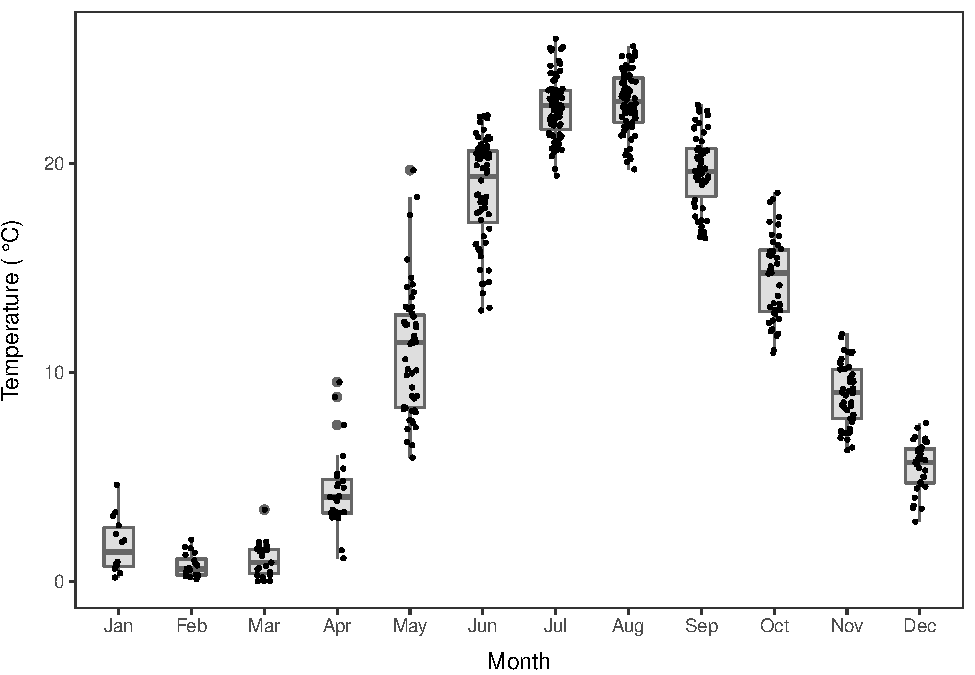
\includegraphics{worstr_files/figure-latex/unnamed-chunk-114-1.pdf}

\hypertarget{next4}{%
\section{Next steps}\label{next4}}

Hopefully this chapter provided you with a basic overview of plotting in R. If you struggled with these exercises, practice them again, or check out some \href{https://danstich.github.io/stich/classes/BIOL217/resources.html}{additional online resources}. In the coming chapters, we will continue to add functionality and complexity to how we use these kinds of plots. We'll look at how to compare two groups within a single plot in \protect\hyperlink{Chapter6}{Chapter 6} when we dive into sampling distributions. And, eventually we will learn how to plot predictions from our statistical model against observed data from Chapter 8 onward.

\hypertarget{Chapter5}{%
\chapter{Sampling distributions in R}\label{Chapter5}}

If we can describe the shape of a probability distribution for a random variable like temperature we can make predictions about the world. Sinister? Maybe. These are temperatures that I simulated from the Hudson River using historical data to estimate parameters of a multivariate normal distribution (muwahahaha).

In this Chapter, we'll talk about probability and probability distributions as a backdrop for the models that we will be working with during the next several chapters. When we describe these from data we have collected, we call them \textbf{sampling distributions}. Probability theory is central to statistical techniques, so it will be important for you to have a pretty firm understanding of this to grab hold of big ideas later on. For now, play along and try to understand how they work. We'll swing back later for a refresher.

In order to complete this Chapter, you will need to have the \texttt{ggplot2}, \texttt{MASS}, and \texttt{Rlab} packages loaded. The only one you should need to install is the \texttt{Rlab} package because \texttt{MASS} is installed when you install R, and we already installed \texttt{ggplot2} with the \texttt{tidyverse} in \protect\hyperlink{Chapter3}{Chapter3}.

I'm going to load these now. In general, it is good practice to put these at the top of the script so we know they are needed.

\begin{Shaded}
\begin{Highlighting}[]
\KeywordTok{library}\NormalTok{(ggplot2)}
\KeywordTok{library}\NormalTok{(MASS)}
\KeywordTok{library}\NormalTok{(Rlab)}
\end{Highlighting}
\end{Shaded}

None of the class data are required to complete this chapter.

\hypertarget{what-are-sampling-distributions}{%
\section{What are sampling distributions?}\label{what-are-sampling-distributions}}

When we talk about sampling distributions, we are talking about the probability that a variable we can measure (e.g.~temperature) takes on some value. In most cases, there is a higher probability that the variable will take on certain values than others. That probability may be governed by any number of processes and thus may assume a number of different shapes with respect to the likelihood of any given value of our variable. The differences in the shapes that we assume, and the mathematical parameters that we use to describe those shapes are called ``probability distributions''. And, when they are estimated from data, they are sampling distributions.

There was a time when biologists were largely restricted to using models that relied heavily on the assumption that the things we measured, and their errors, followed ``normal'' distributions, which you have probably heard of or seen in a scientific paper. This was because of how computationally intensive other methods were. This often led to the use of strictly parametric tools like ANOVA and t-tests, or the use of strictly non-parametric tools like frequency analyses and rank-order methods. While these are still useful techniques in our toolboxes, that time has passed, and now we have access to a wide range of tools that allow us to extend simple parametric and non-parametric tools to relax or change distributional assumptions. We will discuss these throughout the book, but we need to look at the underlying distributions that govern our decisions about which of these tools to use. So, this week we'll look at a few probability distributions that correspond to sampling distributions we frequently encounter in biology. To wrap-up, we will use this new information to talk about how we calculate descriptive statistics such as means and standard deviations from samples.

\hypertarget{probability-distributions-in-r}{%
\section{Probability distributions in R}\label{probability-distributions-in-r}}

R has a number of built-in distribution types, and there are random-number generators associated with most or all of these that will allow us to take random samples from a distribution (like picking numbers out of a hat!). This is useful for data simulation, but is also helpful for us to learn about probability distributions and how their parameters affect the shape, spread, scale, location, etc. of those distributions. We will briefly discuss concepts like skew because of how they can help us think about the assumptions that we are making (or breaking!) in the models that we use.

For this class, we will focus on one major family of distributions and then zero in on a few distributions within this family that you are guaranteed to encounter throughout your career.

\hypertarget{exponential-family}{%
\section{Exponential family}\label{exponential-family}}

Most or all of the distributions we will use for this class come from the \textbf{exponential family} of distributions.

The exponential family is very flexible, and whether you know it or not, it includes most of the distributions one might use to describe every day phenomena. It includes most of the probability distributions with which you are familiar, and many more. Just ask this \emph{very} reliable \href{https://en.wikipedia.org/wiki/Exponential_family}{Wikipedia entry}. Oh, let's face it, you were going there anyway, I just cut out the Google step.

Take a look at the table at the bottom of this Wikipedia page just to get an idea of how many distributions are included within the exponential! Holy cow! We're not going to look at all of these in this class- I just want you to be aware that this is a \textbf{huge} family of specific distributions.

\textbf{Distributions that we'll focus on in this chapter}:

\textbf{1. Continuous distributions}
Normal (Gaussian)
Lognormal
Beta
Uniform
\textbf{2. Discrete distributions}
Bernouli
Binomial
Multinomial
Poisson
Negative binomial

\hypertarget{continuous-distributions}{%
\section{Continuous distributions}\label{continuous-distributions}}

The normal distribution

This is one distribution with which most of you have at least some nodding acquaintance. It is the classic ``bell curve'' that college students once dreaded in upper-level courses. I don't know if it's a thing anymore. Go Google it.

The \textbf{normal distribution} is defined by two parameters:

\begin{enumerate}
\def\labelenumi{\arabic{enumi}.}
\item
  The mean (\(\mu\))
\item
  The variance (\(\sigma^2\))
\end{enumerate}

Let's take a look at what the normal distribution looks like. We'll start with a special one called the standard normal (or \emph{z}) distribution. The standard normal is a normal distribution with a mean of zero and a variance of 1. This one is really cool because the standard deviation (\(\sigma\)) is the square-root of the variance, and in this special case \(\sqrt{1} = 1\), so the variance and standard deviation are equal! And because of this property, and other normal distribution can be converted to a standard normal using z-standardization, which we'll talk about later. How exciting is that?

First, take a sample from a normal distribution:

\begin{Shaded}
\begin{Highlighting}[]
\NormalTok{samp <-}\StringTok{ }\KeywordTok{rnorm}\NormalTok{(}\DataTypeTok{n =} \DecValTok{10000}\NormalTok{, }\DataTypeTok{mean =} \DecValTok{0}\NormalTok{, }\DataTypeTok{sd =} \DecValTok{1}\NormalTok{)}
\end{Highlighting}
\end{Shaded}

Now, plot a histogram using the sick new skills you got in \protect\hyperlink{Chapter4}{Chapter 4}

\begin{Shaded}
\begin{Highlighting}[]
\NormalTok{p <-}\StringTok{ }\KeywordTok{ggplot}\NormalTok{() }\OperatorTok{+}\StringTok{ }
\StringTok{  }\KeywordTok{geom_histogram}\NormalTok{(}\KeywordTok{aes}\NormalTok{(samp), }\DataTypeTok{binwidth =} \DecValTok{1}\NormalTok{) }\OperatorTok{+}\StringTok{ }
\StringTok{  }\KeywordTok{scale_x_continuous}\NormalTok{(}\DataTypeTok{limits=}\KeywordTok{c}\NormalTok{(}\OperatorTok{-}\DecValTok{7}\NormalTok{,}\DecValTok{7}\NormalTok{), }\DataTypeTok{expand =} \KeywordTok{c}\NormalTok{(}\DecValTok{0}\NormalTok{, }\DecValTok{0}\NormalTok{)) }\OperatorTok{+}\StringTok{ }
\StringTok{  }\KeywordTok{scale_y_continuous}\NormalTok{(}\DataTypeTok{expand =} \KeywordTok{c}\NormalTok{(}\DecValTok{0}\NormalTok{, }\DecValTok{1}\NormalTok{)) }\OperatorTok{+}\StringTok{ }
\StringTok{  }\KeywordTok{xlab}\NormalTok{(}\StringTok{"Value"}\NormalTok{) }\OperatorTok{+}
\StringTok{  }\KeywordTok{ylab}\NormalTok{(}\StringTok{"Count"}\NormalTok{) }\OperatorTok{+}
\StringTok{  }\KeywordTok{theme_classic}\NormalTok{() }\OperatorTok{+}
\StringTok{  }\KeywordTok{theme}\NormalTok{(}
    \DataTypeTok{axis.title.x =} \KeywordTok{element_text}\NormalTok{(}\DataTypeTok{vjust =} \DecValTok{-1}\NormalTok{),}
    \DataTypeTok{axis.title.y =} \KeywordTok{element_text}\NormalTok{(}\DataTypeTok{vjust =} \DecValTok{3}\NormalTok{),}
    \DataTypeTok{panel.grid =} \KeywordTok{element_blank}\NormalTok{()}
\NormalTok{  )}
\KeywordTok{print}\NormalTok{(p)}
\end{Highlighting}
\end{Shaded}

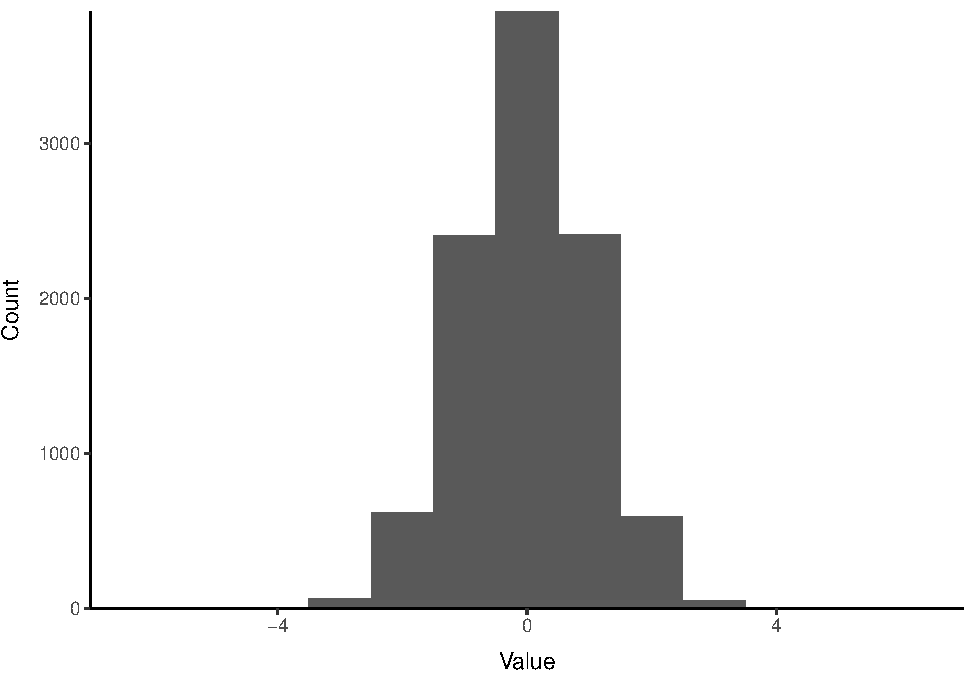
\includegraphics{worstr_files/figure-latex/unnamed-chunk-117-1.pdf}

Pretty!

Because this sample is from a \textbf{continuous} distribution, we might actually wish to represent this distribution with a probability density function. You can think of this as R calculating the relative probability of an given value. It implies a continuous surface, rather than the discrete bins like the histogram. In reality it doesn't matter because at best we chop continuous distributions into tiny little bins when we do things like integrals, and R bases \texttt{binwidth} in histograms off a density function anyway (aaaaah!).

Density plots are a new one for us, so let's try them out. If you scroll back and forth, you'll notice that the code below is basically identical to the histogram above except for labels and scales. We just replaced the histogram geometry (\texttt{geom\_histogram}) with a density-based geometry (\texttt{geom\_density}). Here, we use \texttt{fill\ =\ 1} to trick R into filling the area under the line because we have no grouping variables. By default, this is interpreted as \texttt{\textquotesingle{}black\textquotesingle{}}, so we add an alpha channel for transparency.

\begin{Shaded}
\begin{Highlighting}[]
\NormalTok{p <-}\StringTok{ }\KeywordTok{ggplot}\NormalTok{() }\OperatorTok{+}\StringTok{ }
\StringTok{  }\KeywordTok{geom_density}\NormalTok{(}\KeywordTok{aes}\NormalTok{(samp), }\DataTypeTok{alpha =} \FloatTok{.1}\NormalTok{, }\DataTypeTok{fill =} \DecValTok{1}\NormalTok{) }\OperatorTok{+}\StringTok{ }
\StringTok{  }\KeywordTok{scale_x_continuous}\NormalTok{(}\DataTypeTok{limits =} \KeywordTok{c}\NormalTok{(}\OperatorTok{-}\DecValTok{7}\NormalTok{,}\DecValTok{7}\NormalTok{), }\DataTypeTok{expand =} \KeywordTok{c}\NormalTok{(}\DecValTok{0}\NormalTok{, }\DecValTok{0}\NormalTok{)) }\OperatorTok{+}\StringTok{ }
\StringTok{  }\KeywordTok{scale_y_continuous}\NormalTok{(}\DataTypeTok{expand =} \KeywordTok{c}\NormalTok{(}\DecValTok{0}\NormalTok{, }\DecValTok{0}\NormalTok{)) }\OperatorTok{+}\StringTok{ }
\StringTok{  }\KeywordTok{xlab}\NormalTok{(}\StringTok{"Value"}\NormalTok{) }\OperatorTok{+}
\StringTok{  }\KeywordTok{ylab}\NormalTok{(}\StringTok{"Density"}\NormalTok{) }\OperatorTok{+}
\StringTok{  }\KeywordTok{theme_classic}\NormalTok{() }\OperatorTok{+}
\StringTok{  }\KeywordTok{theme}\NormalTok{(}
    \DataTypeTok{axis.title.x =} \KeywordTok{element_text}\NormalTok{(}\DataTypeTok{vjust =} \DecValTok{-1}\NormalTok{),}
    \DataTypeTok{axis.title.y =} \KeywordTok{element_text}\NormalTok{(}\DataTypeTok{vjust =} \DecValTok{3}\NormalTok{),}
    \DataTypeTok{panel.grid =} \KeywordTok{element_blank}\NormalTok{()}
\NormalTok{  )}
\KeywordTok{print}\NormalTok{(p)}
\end{Highlighting}
\end{Shaded}

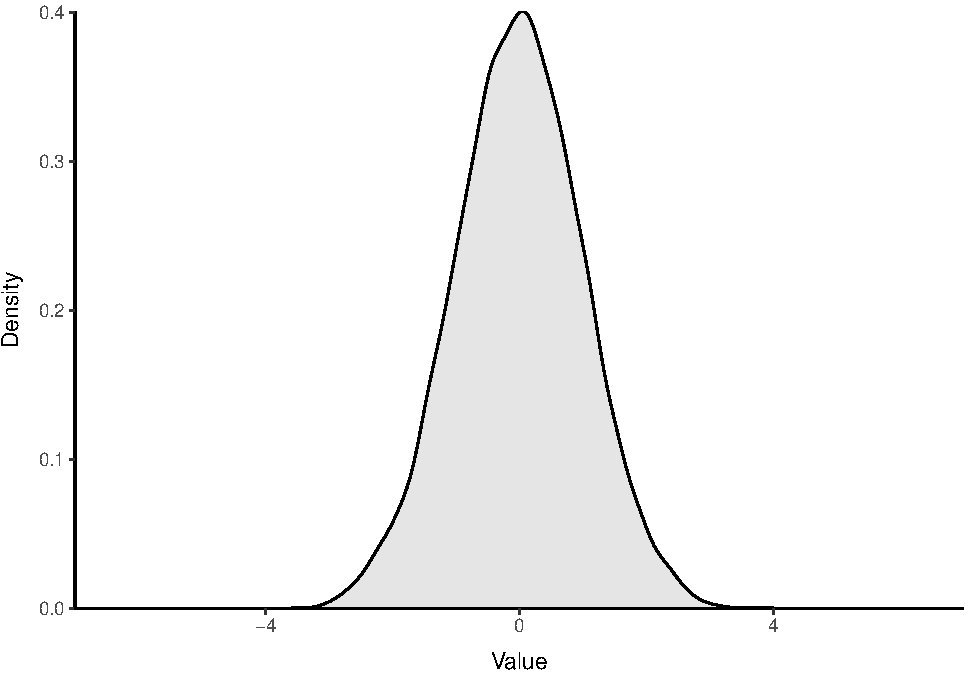
\includegraphics{worstr_files/figure-latex/unnamed-chunk-118-1.pdf}

Excellent use of \texttt{ggplot()} to make a figure that looks like the clunky base graphics. Maybe you can improve on it in the homework assignment?

We can change the parameters of the standard normal to change both the location and the scale of our distribution. The influence of changing the mean, or average, on the location of a distribution is perhaps obvious. But, the influence of variance may be less intuitive, so let's have a look!

Create two more random samples, one with a larger \texttt{sd} and one with a smaller \texttt{sd}, to see how this changes the shape of the distribution:

\begin{Shaded}
\begin{Highlighting}[]
\NormalTok{samp2 <-}\StringTok{ }\KeywordTok{rnorm}\NormalTok{(}\DataTypeTok{n =} \FloatTok{1e4}\NormalTok{, }\DataTypeTok{mean =} \DecValTok{0}\NormalTok{, }\DataTypeTok{sd =} \DecValTok{2}\NormalTok{)}
\NormalTok{samp3 <-}\StringTok{ }\KeywordTok{rnorm}\NormalTok{(}\DataTypeTok{n =} \FloatTok{1e4}\NormalTok{, }\DataTypeTok{mean =} \DecValTok{0}\NormalTok{, }\DataTypeTok{sd =} \FloatTok{.5}\NormalTok{)}
\end{Highlighting}
\end{Shaded}

Let's put them in a data frame with \texttt{samp} so they're easy to plot. We combine all three random samples into one column called \texttt{Value}. Then, we create a column to hold the standard deviation used in each sample (\texttt{Sigma}). If we make that one into a factor, we can use the \texttt{Sigma} columns to plot the samples as separate lines by tweaking our plotting code.

\begin{Shaded}
\begin{Highlighting}[]
\NormalTok{normals <-}\StringTok{ }\KeywordTok{data.frame}\NormalTok{(}
  \DataTypeTok{Value =} \KeywordTok{c}\NormalTok{(samp, samp2, samp3),}
  \DataTypeTok{Sigma =} \KeywordTok{factor}\NormalTok{(}
    \KeywordTok{c}\NormalTok{(}
      \KeywordTok{rep}\NormalTok{(}\DecValTok{1}\NormalTok{, }\KeywordTok{length}\NormalTok{(samp)), }
      \KeywordTok{rep}\NormalTok{(}\DecValTok{2}\NormalTok{, }\KeywordTok{length}\NormalTok{(samp2)), }
      \KeywordTok{rep}\NormalTok{(.}\DecValTok{5}\NormalTok{, }\KeywordTok{length}\NormalTok{(samp3))}
\NormalTok{    )}
\NormalTok{  )}
\NormalTok{)}
\end{Highlighting}
\end{Shaded}

Next, we can just add these to the plot to compare the sampling distributions. This time, we tell R to fill the area under our lines based on sample ID with a default color scheme by saying \texttt{fill\ =\ Sigma} in our \texttt{ggplot()} call. We also added \texttt{color\ =\ Sigma} to make the lines the same default colors. Remember, you can specify your own.

\begin{Shaded}
\begin{Highlighting}[]
\NormalTok{p <-}\StringTok{ }\KeywordTok{ggplot}\NormalTok{(}\DataTypeTok{data =}\NormalTok{ normals, }
            \KeywordTok{aes}\NormalTok{(}\DataTypeTok{x =}\NormalTok{ Value, }\DataTypeTok{group =}\NormalTok{ Sigma, }\DataTypeTok{fill =}\NormalTok{ Sigma, }\DataTypeTok{color =}\NormalTok{ Sigma)) }\OperatorTok{+}
\StringTok{  }\KeywordTok{geom_density}\NormalTok{(}\DataTypeTok{adjust =} \FloatTok{1.5}\NormalTok{, }\DataTypeTok{alpha =} \FloatTok{.4}\NormalTok{) }\OperatorTok{+}
\StringTok{  }\KeywordTok{scale_x_continuous}\NormalTok{(}\DataTypeTok{limits =} \KeywordTok{c}\NormalTok{(}\OperatorTok{-}\DecValTok{7}\NormalTok{, }\DecValTok{7}\NormalTok{), }\DataTypeTok{expand =} \KeywordTok{c}\NormalTok{(}\DecValTok{0}\NormalTok{, }\DecValTok{0}\NormalTok{)) }\OperatorTok{+}\StringTok{ }
\StringTok{  }\KeywordTok{scale_y_continuous}\NormalTok{(}\DataTypeTok{expand =} \KeywordTok{c}\NormalTok{(}\DecValTok{0}\NormalTok{, }\DecValTok{0}\NormalTok{)) }\OperatorTok{+}\StringTok{ }
\StringTok{  }\KeywordTok{xlab}\NormalTok{(}\StringTok{"Value"}\NormalTok{) }\OperatorTok{+}
\StringTok{  }\KeywordTok{ylab}\NormalTok{(}\StringTok{"Density"}\NormalTok{) }\OperatorTok{+}
\StringTok{  }\KeywordTok{theme_classic}\NormalTok{() }\OperatorTok{+}
\StringTok{  }\KeywordTok{theme}\NormalTok{(}
    \DataTypeTok{axis.title.x =} \KeywordTok{element_text}\NormalTok{(}\DataTypeTok{vjust =} \DecValTok{-1}\NormalTok{),}
    \DataTypeTok{axis.title.y =} \KeywordTok{element_text}\NormalTok{(}\DataTypeTok{vjust =} \DecValTok{3}\NormalTok{),}
    \DataTypeTok{panel.grid =} \KeywordTok{element_blank}\NormalTok{()}
\NormalTok{  )}
\KeywordTok{print}\NormalTok{(p)}
\end{Highlighting}
\end{Shaded}

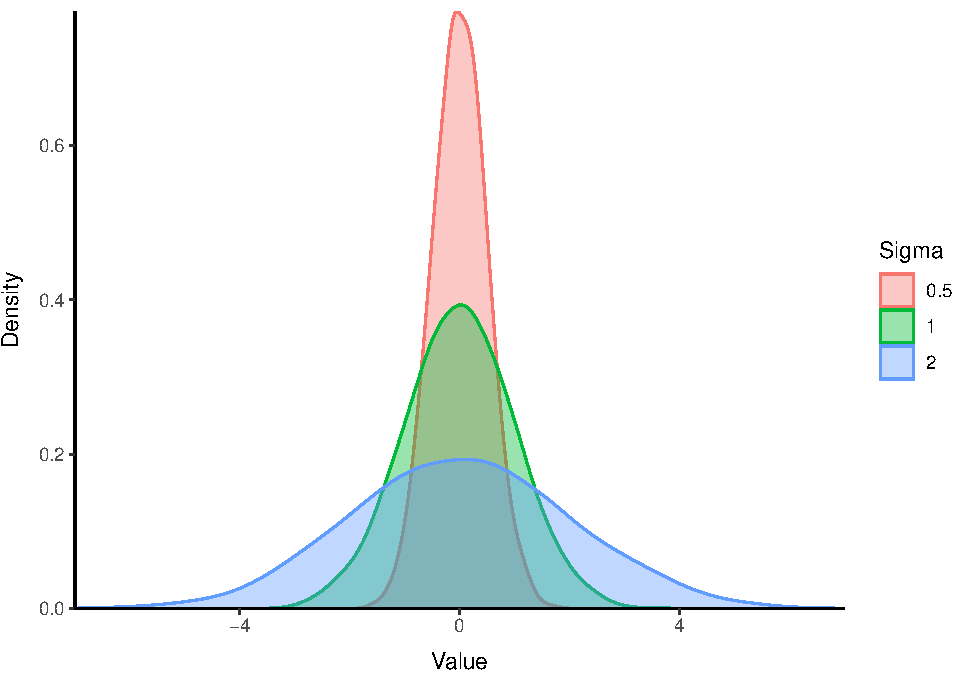
\includegraphics{worstr_files/figure-latex/unnamed-chunk-121-1.pdf}

The blue polygon in the plot above shows a distribution with greater variance than our z distribution (green). The red polygon shows a distribution with a smaller variance. Hopefully this helps demonstrate how variance influences the scale of the distribution.

\hypertarget{the-lognormal-distribution}{%
\subsection{The lognormal distribution}\label{the-lognormal-distribution}}

The \textbf{lognormal distribution} is a probability distribution that assumes our random variable is normally distributed on the \textbf{log scale}. This assumption allows us to incorporate \textbf{skew} into the normal distribution and change the location and scale of the normal distribution by transforming the parameters (\(\mu\) and \(\sigma\)) onto the log scale. This is one of the more common data transformations that you will run into, e.g.: ``We log-transformed the data to achieve normality\ldots{}''. One of the other reasons for that is that all values (positive or negative) transformed from the log to the real scale are positive, so it helps prevent us from making negative predictions about phenomena or variables that can't be less than zero.

Let's take a look at how changes to the mean change the location of this distribution:

\begin{Shaded}
\begin{Highlighting}[]
\CommentTok{# Create random samples from log-normal}
\CommentTok{# distributions with different means}
\NormalTok{samp1 <-}\StringTok{ }\KeywordTok{rlnorm}\NormalTok{(}\DataTypeTok{n=}\FloatTok{1e4}\NormalTok{, }\DataTypeTok{mean=}\DecValTok{0}\NormalTok{, }\DataTypeTok{sd=}\DecValTok{1}\NormalTok{)}
\NormalTok{samp2 <-}\StringTok{ }\KeywordTok{rlnorm}\NormalTok{(}\DataTypeTok{n=}\FloatTok{1e4}\NormalTok{, }\DataTypeTok{mean=}\DecValTok{1}\NormalTok{, }\DataTypeTok{sd=}\DecValTok{1}\NormalTok{)}
\NormalTok{samp3 <-}\StringTok{ }\KeywordTok{rlnorm}\NormalTok{(}\DataTypeTok{n=}\FloatTok{1e4}\NormalTok{, }\DataTypeTok{mean=}\DecValTok{2}\NormalTok{, }\DataTypeTok{sd=}\DecValTok{1}\NormalTok{)}

\CommentTok{# Put them in a data frame with the values}
\CommentTok{# of the means used to create them}
\NormalTok{lognormals <-}\StringTok{ }\KeywordTok{data.frame}\NormalTok{(}
  \DataTypeTok{Value =} \KeywordTok{c}\NormalTok{(samp, samp2, samp3),}
  \DataTypeTok{X_bar =} \KeywordTok{factor}\NormalTok{(}
    \KeywordTok{c}\NormalTok{(}
      \KeywordTok{rep}\NormalTok{(}\DecValTok{0}\NormalTok{, }\KeywordTok{length}\NormalTok{(samp)), }
      \KeywordTok{rep}\NormalTok{(}\DecValTok{1}\NormalTok{, }\KeywordTok{length}\NormalTok{(samp2)), }
      \KeywordTok{rep}\NormalTok{(}\DecValTok{2}\NormalTok{, }\KeywordTok{length}\NormalTok{(samp3))}
\NormalTok{    )}
\NormalTok{  )}
\NormalTok{)}
\end{Highlighting}
\end{Shaded}

Now you can plot these using the code above with a couple of modifications to show how the mean of the log-normal distribution influences the location.

\begin{Shaded}
\begin{Highlighting}[]
\NormalTok{p <-}\StringTok{ }\KeywordTok{ggplot}\NormalTok{(}\DataTypeTok{data =}\NormalTok{ lognormals,}
            \KeywordTok{aes}\NormalTok{(}\DataTypeTok{x =}\NormalTok{ Value, }\DataTypeTok{group =}\NormalTok{ X_bar, }\DataTypeTok{fill =}\NormalTok{ X_bar, }\DataTypeTok{color =}\NormalTok{ X_bar)) }\OperatorTok{+}
\StringTok{  }\KeywordTok{geom_density}\NormalTok{(}\DataTypeTok{adjust =} \FloatTok{1.5}\NormalTok{, }\DataTypeTok{alpha =} \FloatTok{.4}\NormalTok{) }\OperatorTok{+}
\StringTok{  }\KeywordTok{scale_x_continuous}\NormalTok{(}\DataTypeTok{limits =}\KeywordTok{c}\NormalTok{(}\DecValTok{0}\NormalTok{, }\DecValTok{50}\NormalTok{), }\DataTypeTok{expand =} \KeywordTok{c}\NormalTok{(}\DecValTok{0}\NormalTok{, }\DecValTok{0}\NormalTok{)) }\OperatorTok{+}\StringTok{ }
\StringTok{  }\KeywordTok{scale_y_continuous}\NormalTok{(}\DataTypeTok{expand =} \KeywordTok{c}\NormalTok{(}\DecValTok{0}\NormalTok{, }\DecValTok{0}\NormalTok{)) }\OperatorTok{+}\StringTok{ }
\StringTok{  }\KeywordTok{xlab}\NormalTok{(}\StringTok{"Value"}\NormalTok{) }\OperatorTok{+}
\StringTok{  }\KeywordTok{ylab}\NormalTok{(}\StringTok{"Density"}\NormalTok{) }\OperatorTok{+}
\StringTok{  }\KeywordTok{theme_classic}\NormalTok{() }\OperatorTok{+}
\StringTok{  }\KeywordTok{theme}\NormalTok{(}
    \DataTypeTok{axis.title.x =} \KeywordTok{element_text}\NormalTok{(}\DataTypeTok{vjust =} \DecValTok{-1}\NormalTok{),}
    \DataTypeTok{axis.title.y =} \KeywordTok{element_text}\NormalTok{(}\DataTypeTok{vjust =} \DecValTok{3}\NormalTok{),}
    \DataTypeTok{panel.grid =} \KeywordTok{element_blank}\NormalTok{()}
\NormalTok{  )}
\KeywordTok{print}\NormalTok{(p)}
\end{Highlighting}
\end{Shaded}

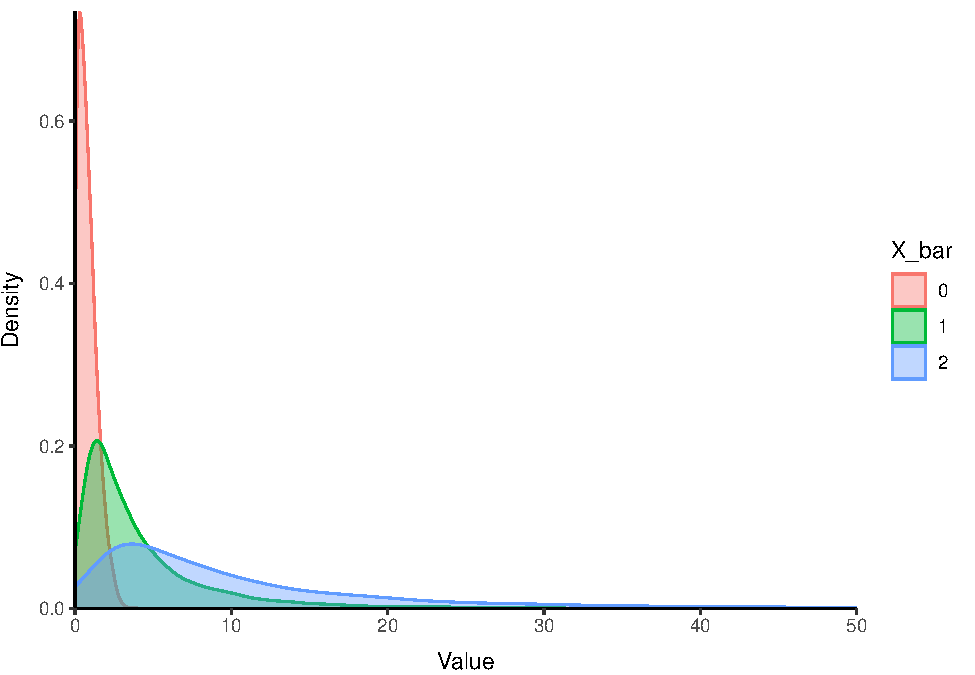
\includegraphics{worstr_files/figure-latex/unnamed-chunk-123-1.pdf}

You can see that the relative scale of these three distributions is similar, but the location shifts to the right on our x-axis as the value of \texttt{X\_bar} (the mean) increases. Note also how this affects \emph{kurtosis}.

\hypertarget{the-beta-distribution}{%
\subsection{The beta distribution}\label{the-beta-distribution}}

The \textbf{beta distribution} is a probability distribution that is constrained to the interval {[}0, 1{]}. But, it is incredibly flexible in its parameterization, and as a result is very useful for stochastic simulation of variables on the probability scale, such as survival.

The parameters of the beta distribution are \(\alpha\) and \(\beta\), or commonly \texttt{a} and \texttt{b} or \texttt{shape\ 1} and \texttt{shape\ 2} in R. Within this distribution, \(\alpha\) pushes the distribution to the right (toward 1), and \(\beta\) pushes the distribution back toward the left (toward 0). The relative magnitude of \(\alpha\) and \(\beta\) determine the location, shape, and scale of the probability distribution for our random variable. When \(\alpha\) and \(\beta\) are equal, and greater than 1, the beta distribution looks like a normal distribution within the interval {[}0, 1{]}.

Let's take a look:

\begin{Shaded}
\begin{Highlighting}[]
\CommentTok{# Simulate random values from 3 different beta distributions}
\CommentTok{# so we can compare them}
\NormalTok{samp1 <-}\StringTok{ }\KeywordTok{rbeta}\NormalTok{(}\DataTypeTok{n=}\FloatTok{1e4}\NormalTok{, }\DataTypeTok{shape1=}\DecValTok{50}\NormalTok{, }\DataTypeTok{shape2=}\DecValTok{50}\NormalTok{)}
\NormalTok{samp2 <-}\StringTok{ }\KeywordTok{rbeta}\NormalTok{(}\DataTypeTok{n=}\FloatTok{1e4}\NormalTok{, }\DataTypeTok{shape1=}\DecValTok{50}\NormalTok{, }\DataTypeTok{shape2=}\DecValTok{100}\NormalTok{)     }
\NormalTok{samp3 <-}\StringTok{ }\KeywordTok{rbeta}\NormalTok{(}\DataTypeTok{n=}\FloatTok{1e4}\NormalTok{, }\DataTypeTok{shape1=}\DecValTok{500}\NormalTok{, }\DataTypeTok{shape2=}\DecValTok{250}\NormalTok{) }

\CommentTok{# Put them in a data frame with the values}
\CommentTok{# of the means used to create them. I am }
\CommentTok{# using "theta" because often that is how we}
\CommentTok{# refer collectively to a group of parameters}
\NormalTok{betas <-}\StringTok{ }\KeywordTok{data.frame}\NormalTok{(}
  \DataTypeTok{Value =} \KeywordTok{c}\NormalTok{(samp, samp2, samp3),}
  \DataTypeTok{theta =} \KeywordTok{factor}\NormalTok{(}
    \KeywordTok{c}\NormalTok{(}
      \KeywordTok{rep}\NormalTok{(}\StringTok{'a = 50, b = 50'}\NormalTok{, }\KeywordTok{length}\NormalTok{(samp)), }
      \KeywordTok{rep}\NormalTok{(}\StringTok{'a = 50, b = 100'}\NormalTok{, }\KeywordTok{length}\NormalTok{(samp2)), }
      \KeywordTok{rep}\NormalTok{(}\StringTok{'a = 500, b = 250'}\NormalTok{, }\KeywordTok{length}\NormalTok{(samp3))}
\NormalTok{    )}
\NormalTok{  )}
\NormalTok{)}
\end{Highlighting}
\end{Shaded}

And then, we can plot them just like we did above. Copy and paste it - change what you need. Isn't code great?. Just don't forget to change the scale and the data in the plotting code!

\begin{Shaded}
\begin{Highlighting}[]
\NormalTok{p <-}\StringTok{ }\KeywordTok{ggplot}\NormalTok{(}\DataTypeTok{data =}\NormalTok{ betas,}
            \KeywordTok{aes}\NormalTok{(}\DataTypeTok{x =}\NormalTok{ Value, }\DataTypeTok{group =}\NormalTok{ theta, }\DataTypeTok{fill =}\NormalTok{ theta, }\DataTypeTok{color =}\NormalTok{ theta)) }\OperatorTok{+}
\StringTok{  }\KeywordTok{geom_density}\NormalTok{(}\DataTypeTok{adjust =} \FloatTok{1.5}\NormalTok{, }\DataTypeTok{alpha =} \FloatTok{.4}\NormalTok{) }\OperatorTok{+}
\StringTok{  }\KeywordTok{scale_x_continuous}\NormalTok{(}\DataTypeTok{limits =}\KeywordTok{c}\NormalTok{(}\DecValTok{0}\NormalTok{, }\DecValTok{1}\NormalTok{), }\DataTypeTok{expand =} \KeywordTok{c}\NormalTok{(}\DecValTok{0}\NormalTok{, }\DecValTok{0}\NormalTok{)) }\OperatorTok{+}\StringTok{ }
\StringTok{  }\KeywordTok{scale_y_continuous}\NormalTok{(}\DataTypeTok{expand =} \KeywordTok{c}\NormalTok{(}\DecValTok{0}\NormalTok{, }\DecValTok{0}\NormalTok{)) }\OperatorTok{+}\StringTok{ }
\StringTok{  }\KeywordTok{xlab}\NormalTok{(}\StringTok{"Value"}\NormalTok{) }\OperatorTok{+}
\StringTok{  }\KeywordTok{ylab}\NormalTok{(}\StringTok{"Density"}\NormalTok{) }\OperatorTok{+}
\StringTok{  }\KeywordTok{theme_classic}\NormalTok{() }\OperatorTok{+}
\StringTok{  }\KeywordTok{theme}\NormalTok{(}
    \DataTypeTok{axis.title.x =} \KeywordTok{element_text}\NormalTok{(}\DataTypeTok{vjust =} \DecValTok{-1}\NormalTok{),}
    \DataTypeTok{axis.title.y =} \KeywordTok{element_text}\NormalTok{(}\DataTypeTok{vjust =} \DecValTok{3}\NormalTok{),}
    \DataTypeTok{panel.grid =} \KeywordTok{element_blank}\NormalTok{()}
\NormalTok{  )}
\KeywordTok{print}\NormalTok{(p)}
\end{Highlighting}
\end{Shaded}

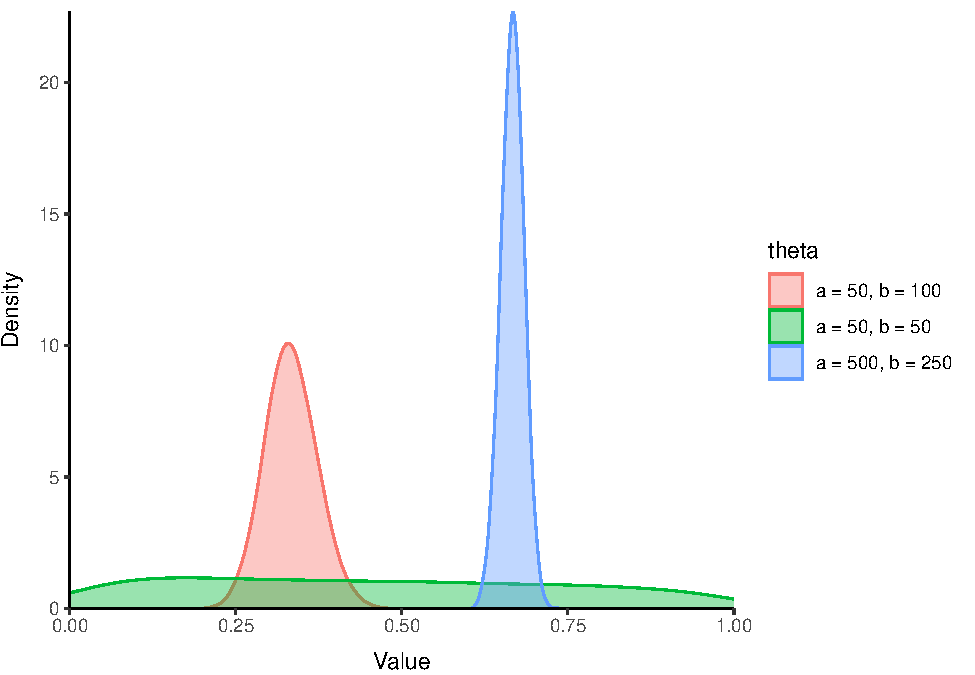
\includegraphics{worstr_files/figure-latex/unnamed-chunk-125-1.pdf}

Play around with these to see what kind of cool shapes you can make and where they are located within the range between zero and one.

\hypertarget{discrete-distributions}{%
\section{Discrete distributions}\label{discrete-distributions}}

\textbf{Discrete} probability distributions are useful for situations in which our random variable of interest can only take specific values within the interval of interest. For example, this might include age, counts, pass/fail, or any number of conceivable categories. As a result, these require a slightly different treatment of probability as a discrete, rather than continuous phenomenon. (Think back to our histogram that we started with in this chapter.)

\hypertarget{bernoulli}{%
\subsection{Bernoulli}\label{bernoulli}}

The \textbf{Bernoulli distribution} is a special case of the binomial distribution with a single trial (see below for clarification). Bernoulli outcomes are those for which the variable we are measuring can take on one of two values: a one or a zero. This distribution is useful for visualizing processes such as coin flips, yes/no responses, live/dead endpoints in lab studies, and a number of other very interesting phenomena. The Bernoulli distribution has a single parameter: the probability of success, but the number of successful outcomes is also governed by sample size: \emph{n}, which R calls \texttt{size} because \texttt{n} was already taken.

We can simulate data from a Bernoulli distribution in one of two ways in R.

The ``old-school'' way of doing this was to draw from a binomial with a single \textbf{trial}. Here we randomly draw a single sample from a binomial with a single trial, and a 50\% chance of success. We'll use the example of hatching chicken eggs with some probability of success. If you are boring, you can think about flipping coins, too!

We'll start with one chicken egg that has a 50\% chance of successfully hatching (probability of success = 0.50).

\begin{Shaded}
\begin{Highlighting}[]
\KeywordTok{rbinom}\NormalTok{(}\DataTypeTok{n=}\DecValTok{1}\NormalTok{, }\DataTypeTok{size=}\DecValTok{1}\NormalTok{, }\DataTypeTok{prob=}\NormalTok{.}\DecValTok{5}\NormalTok{)}
\end{Highlighting}
\end{Shaded}

\begin{verbatim}
## [1] 0
\end{verbatim}

There is also a function called \texttt{rbern} in the \texttt{Rlab} package that simplifies this for the specific case of a Bernoulli.

Let's do it again with that function:

\begin{Shaded}
\begin{Highlighting}[]
\CommentTok{# Hatch one egg with 50% success rate}
\KeywordTok{rbern}\NormalTok{(}\DataTypeTok{n =} \DecValTok{1}\NormalTok{, }\DataTypeTok{prob =} \FloatTok{.5}\NormalTok{)}
\end{Highlighting}
\end{Shaded}

\begin{verbatim}
## [1] 0
\end{verbatim}

Or we could hatch a whole bunch of eggs:

\begin{Shaded}
\begin{Highlighting}[]
\CommentTok{# Hatch ten eggs, each with p = 0.5}
\KeywordTok{rbern}\NormalTok{(}\DataTypeTok{n =} \DecValTok{10}\NormalTok{, }\DataTypeTok{prob =} \FloatTok{.5}\NormalTok{)}
\end{Highlighting}
\end{Shaded}

\begin{verbatim}
##  [1] 1 0 0 0 0 0 0 1 1 0
\end{verbatim}

Then, we could even count how many of those were successful. Do you remember how to do that? There are several different ways. You'll have to come up with one for the homework assignment (hint: see \protect\hyperlink{Chapter2}{Chapter 2}).

\hypertarget{binomial}{%
\subsection{Binomial}\label{binomial}}

The \textbf{binomial distribution} is pretty similar to the Bernoulli distribution. In fact, the Bernoulli is just a special kind of binomial. The binomial includes a parameter called \(N\) (\texttt{size} in R) which corresponds to a number of trials per sample. We assume that this is 1 in the case of Bernoulli. In most cases in biology, it will suffice to use the Bernoulli, but for modeling we will want to understand the binomial for things like random stratified designs and nested models that rely on the use of binomial distribution. Later in your career, you might even get into cool models that estimate \(N\) as a latent state to estimate population size (for example). Plus, using the binomial is way faster and can be more precise for certain regression applications {[}okay, that one should probably have a citation, but this is The Worst Stats Text eveR, so go Google it{]}.

To sample data from a binomial distribution, we can use \texttt{rbinom} from base R. In this example we tell R that we want 10 samples (\texttt{n}) from a binomial distribution that has 10 trials (\texttt{size}) and a probability of success (\texttt{prob}) of 0.5. This is like hatching ten eggs from each of ten chickens instead of just one chicken laying ten eggs.

\begin{Shaded}
\begin{Highlighting}[]
\CommentTok{# Take a random draw of 10 samples}
\CommentTok{# from a binomial distribution with 10 trials}
\CommentTok{# and probability of success equal to 0.50}
\KeywordTok{rbinom}\NormalTok{(}\DataTypeTok{n=}\DecValTok{10}\NormalTok{, }\DataTypeTok{size=}\DecValTok{10}\NormalTok{, }\DataTypeTok{prob=}\FloatTok{0.5}\NormalTok{)}
\end{Highlighting}
\end{Shaded}

\begin{verbatim}
##  [1] 5 4 2 6 4 2 6 5 6 5
\end{verbatim}

Remember as you look through these that your numbers should look different than mine (at least most of the time) because these are being generated randomly.

\hypertarget{multinomial}{%
\subsection{Multinomial}\label{multinomial}}

The \textbf{multinomial distribution} is a further generalization of the Binomial and Bernoulli distributions. Here, there are one or more possible categorical outcomes (states), and the probability of each one occurring is specified individually \textbf{but all of them must sum to one}. The categories are, in this case, assumed to be a \textbf{mutually exclusive} and \textbf{exhaustive} set of possible outcomes.

We can use the multinomial distribution to randomly sample from categories (imagine our response variable is a categorical variable, like the names of the students in this class).

To do this, we need to read in the \texttt{s\_names.csv} file from our \texttt{data} folder that is definitely in your working directory (\textbf{remember to set your working directory first}).

Read in the data file with \texttt{stringsAsFactors\ =\ FALSE} for purposes of demonstrating with categorical variables (not factors).

\begin{Shaded}
\begin{Highlighting}[]
\NormalTok{s_names <-}\StringTok{ }\KeywordTok{read.csv}\NormalTok{(}\StringTok{'data/s_names.csv'}\NormalTok{, }\DataTypeTok{stringsAsFactors =} \OtherTok{FALSE}\NormalTok{)}
\end{Highlighting}
\end{Shaded}

Next, let's assign the variable \texttt{name} in \texttt{s\_names} to a vector for simplicity.

\begin{Shaded}
\begin{Highlighting}[]
\NormalTok{name <-}\StringTok{ }\NormalTok{s_names}\OperatorTok{$}\NormalTok{name}
\end{Highlighting}
\end{Shaded}

Then, we can assign a uniform probability of drawing any given name if we divide one by the number of names.

\begin{Shaded}
\begin{Highlighting}[]
\CommentTok{# Calculate probability of getting a given }
\CommentTok{# name based on the length of the vector}
\NormalTok{prob_each <-}\StringTok{ }\DecValTok{1} \OperatorTok{/}\StringTok{ }\KeywordTok{length}\NormalTok{(name)}

\CommentTok{# Repeat this probability for each }
\CommentTok{# name in our vector of names}
\NormalTok{probs <-}\StringTok{ }\KeywordTok{rep}\NormalTok{(prob_each, }\DataTypeTok{times =} \KeywordTok{length}\NormalTok{(name))      }
\NormalTok{probs      }
\end{Highlighting}
\end{Shaded}

\begin{verbatim}
##  [1] 0.03846154 0.03846154 0.03846154 0.03846154 0.03846154 0.03846154
##  [7] 0.03846154 0.03846154 0.03846154 0.03846154 0.03846154 0.03846154
## [13] 0.03846154 0.03846154 0.03846154 0.03846154 0.03846154 0.03846154
## [19] 0.03846154 0.03846154 0.03846154 0.03846154 0.03846154 0.03846154
## [25] 0.03846154 0.03846154
\end{verbatim}

This shows us that the probability of drawing any of the individual names is \texttt{\{r\ prob\_each\}}.

Now, we can sample from a multinomial distribution using our objects. Here we are taking 5 samples from the distribution, each time we sample there is only one trial, and we are sampling with the 26 probabilities above.

Have a look:

\begin{Shaded}
\begin{Highlighting}[]
\KeywordTok{rmultinom}\NormalTok{(}\DataTypeTok{n=}\DecValTok{5}\NormalTok{, }\DataTypeTok{size=}\DecValTok{1}\NormalTok{, }\DataTypeTok{prob=}\NormalTok{probs)}
\end{Highlighting}
\end{Shaded}

\begin{verbatim}
##       [,1] [,2] [,3] [,4] [,5]
##  [1,]    0    0    0    0    0
##  [2,]    0    0    0    1    0
##  [3,]    0    0    0    0    0
##  [4,]    0    0    0    0    0
##  [5,]    0    0    0    0    0
##  [6,]    0    0    0    0    0
##  [7,]    0    0    0    0    0
##  [8,]    0    0    0    0    0
##  [9,]    0    0    0    0    0
## [10,]    0    0    0    0    0
## [11,]    0    0    0    0    0
## [12,]    0    0    0    0    0
## [13,]    1    0    0    0    0
## [14,]    0    0    0    0    0
## [15,]    0    0    0    0    0
## [16,]    0    0    0    0    1
## [17,]    0    0    0    0    0
## [18,]    0    1    0    0    0
## [19,]    0    0    1    0    0
## [20,]    0    0    0    0    0
## [21,]    0    0    0    0    0
## [22,]    0    0    0    0    0
## [23,]    0    0    0    0    0
## [24,]    0    0    0    0    0
## [25,]    0    0    0    0    0
## [26,]    0    0    0    0    0
\end{verbatim}

\textbf{WHOA} a matrix??!!! \textbf{What does it all mean}?

Take a step back, breathe, and think about this. The rows in this matrix are you and your classmates. If we took one random sample from the multinomial distribution, it would look like this:

\begin{Shaded}
\begin{Highlighting}[]
\CommentTok{# Take a single sample from}
\CommentTok{# the list of student names    }
\KeywordTok{rmultinom}\NormalTok{(}\DataTypeTok{n=}\DecValTok{1}\NormalTok{, }\DataTypeTok{size=}\DecValTok{1}\NormalTok{, }\DataTypeTok{prob=}\NormalTok{probs)}
\end{Highlighting}
\end{Shaded}

\begin{verbatim}
##       [,1]
##  [1,]    0
##  [2,]    0
##  [3,]    0
##  [4,]    0
##  [5,]    0
##  [6,]    0
##  [7,]    0
##  [8,]    0
##  [9,]    0
## [10,]    0
## [11,]    0
## [12,]    0
## [13,]    0
## [14,]    0
## [15,]    1
## [16,]    0
## [17,]    0
## [18,]    0
## [19,]    0
## [20,]    0
## [21,]    0
## [22,]    0
## [23,]    0
## [24,]    0
## [25,]    0
## [26,]    0
\end{verbatim}

Here, we pulled a single sample from the distribution, and probability of sampling a given individual was 0.04 (1/26). If it makes it easier, we can put your names next to it:

\begin{Shaded}
\begin{Highlighting}[]
\KeywordTok{cbind}\NormalTok{(name, }\KeywordTok{rmultinom}\NormalTok{(}\DataTypeTok{n=}\DecValTok{1}\NormalTok{, }\DataTypeTok{size=}\DecValTok{1}\NormalTok{, }\DataTypeTok{prob=}\NormalTok{probs))}
\end{Highlighting}
\end{Shaded}

\begin{verbatim}
##       name             
##  [1,] "Ava"         "0"
##  [2,] "Dillon"      "1"
##  [3,] "Delaney"     "0"
##  [4,] "Manolo"      "0"
##  [5,] "Sarah"       "0"
##  [6,] "Shannon"     "0"
##  [7,] "Olivia"      "0"
##  [8,] "Ebony"       "0"
##  [9,] "Julia"       "0"
## [10,] "Davi"        "0"
## [11,] "Gabrielle"   "0"
## [12,] "Jordan"      "0"
## [13,] "Tayler"      "0"
## [14,] "Summer"      "0"
## [15,] "Leah"        "0"
## [16,] "Christine"   "0"
## [17,] "Ashley"      "0"
## [18,] "Katherine"   "0"
## [19,] "James"       "0"
## [20,] "Emily"       "0"
## [21,] "Cassidy"     "0"
## [22,] "Maximillion" "0"
## [23,] "Sierra"      "0"
## [24,] "Kyle"        "0"
## [25,] "Diana"       "0"
## [26,] "Amanda"      "0"
\end{verbatim}

Now, if I was calling on you randomly in class, after 10 questions, the spread of people who would have participated in class might look like this (or whatever you got - remember, it is random):

\begin{Shaded}
\begin{Highlighting}[]
\KeywordTok{cbind}\NormalTok{(name, }\KeywordTok{rmultinom}\NormalTok{(}\DataTypeTok{n=}\DecValTok{10}\NormalTok{, }\DataTypeTok{size=}\DecValTok{1}\NormalTok{, }\DataTypeTok{prob=}\NormalTok{probs))}
\end{Highlighting}
\end{Shaded}

\begin{verbatim}
##       name                                                 
##  [1,] "Ava"         "0" "0" "0" "1" "0" "0" "1" "0" "0" "0"
##  [2,] "Dillon"      "0" "0" "0" "0" "0" "0" "0" "0" "1" "0"
##  [3,] "Delaney"     "0" "0" "0" "0" "0" "0" "0" "0" "0" "0"
##  [4,] "Manolo"      "0" "0" "0" "0" "0" "0" "0" "0" "0" "0"
##  [5,] "Sarah"       "0" "0" "0" "0" "0" "0" "0" "0" "0" "0"
##  [6,] "Shannon"     "0" "0" "0" "0" "0" "1" "0" "0" "0" "0"
##  [7,] "Olivia"      "1" "0" "0" "0" "0" "0" "0" "0" "0" "0"
##  [8,] "Ebony"       "0" "0" "0" "0" "0" "0" "0" "0" "0" "0"
##  [9,] "Julia"       "0" "0" "0" "0" "0" "0" "0" "0" "0" "0"
## [10,] "Davi"        "0" "0" "0" "0" "0" "0" "0" "0" "0" "0"
## [11,] "Gabrielle"   "0" "0" "0" "0" "0" "0" "0" "0" "0" "0"
## [12,] "Jordan"      "0" "0" "0" "0" "0" "0" "0" "0" "0" "0"
## [13,] "Tayler"      "0" "0" "0" "0" "0" "0" "0" "0" "0" "0"
## [14,] "Summer"      "0" "0" "0" "0" "0" "0" "0" "0" "0" "0"
## [15,] "Leah"        "0" "0" "0" "0" "0" "0" "0" "0" "0" "0"
## [16,] "Christine"   "0" "0" "0" "0" "0" "0" "0" "0" "0" "1"
## [17,] "Ashley"      "0" "0" "0" "0" "0" "0" "0" "0" "0" "0"
## [18,] "Katherine"   "0" "0" "0" "0" "0" "0" "0" "0" "0" "0"
## [19,] "James"       "0" "0" "0" "0" "1" "0" "0" "0" "0" "0"
## [20,] "Emily"       "0" "0" "0" "0" "0" "0" "0" "0" "0" "0"
## [21,] "Cassidy"     "0" "0" "0" "0" "0" "0" "0" "0" "0" "0"
## [22,] "Maximillion" "0" "0" "0" "0" "0" "0" "0" "1" "0" "0"
## [23,] "Sierra"      "0" "0" "0" "0" "0" "0" "0" "0" "0" "0"
## [24,] "Kyle"        "0" "0" "0" "0" "0" "0" "0" "0" "0" "0"
## [25,] "Diana"       "0" "1" "0" "0" "0" "0" "0" "0" "0" "0"
## [26,] "Amanda"      "0" "0" "1" "0" "0" "0" "0" "0" "0" "0"
\end{verbatim}

Taking this one step further, we could just draw a name and stop looking at these ugly (no but really they are \textbf{awesome}!) matrices:

\begin{Shaded}
\begin{Highlighting}[]
\NormalTok{name[}\KeywordTok{which}\NormalTok{(}\KeywordTok{rmultinom}\NormalTok{(}\DataTypeTok{n=}\DecValTok{1}\NormalTok{, }\DataTypeTok{size=}\DecValTok{1}\NormalTok{, }\DataTypeTok{prob=}\NormalTok{probs)}\OperatorTok{>}\DecValTok{0}\NormalTok{)]}
\end{Highlighting}
\end{Shaded}

\begin{verbatim}
## [1] "Delaney"
\end{verbatim}

And now we have a way to randomly select an individual based on a multinomial distribution. What fun!

\hypertarget{poisson}{%
\subsection{Poisson}\label{poisson}}

The \textbf{Poisson distribution} is used for counts or other integer data. This distribution is widely used (and just as widely misused!) for its ability to account for a large number of biological and ecological processes in the models that we will discuss this semester. The Poisson distribution has a single parameter, \(\lambda\), which is both the mean and the variance of the distribution. So, despite its utility, the distribution is relatively inflexible with respect to shape and spread. \textbf{Fun fact}: this distribution was made widely known by a Russian economist to predict the number of soldiers who were accidentally killed from being kicked by horses in the Prussian army each year. It is named, however, after French mathematician Siméon Denis Poisson. {[}fails to provide citations for any of this{]}

Take a look at how the distribution changes when you change \(\lambda\), and you will get an idea of how this one works. It is probably the most straightforward of any we've considered.

\begin{Shaded}
\begin{Highlighting}[]
\KeywordTok{hist}\NormalTok{(}\KeywordTok{rpois}\NormalTok{(}\DataTypeTok{n=}\FloatTok{1e4}\NormalTok{, }\DataTypeTok{lambda=}\DecValTok{100}\NormalTok{), }\DataTypeTok{main=}\StringTok{''}\NormalTok{)}
\end{Highlighting}
\end{Shaded}

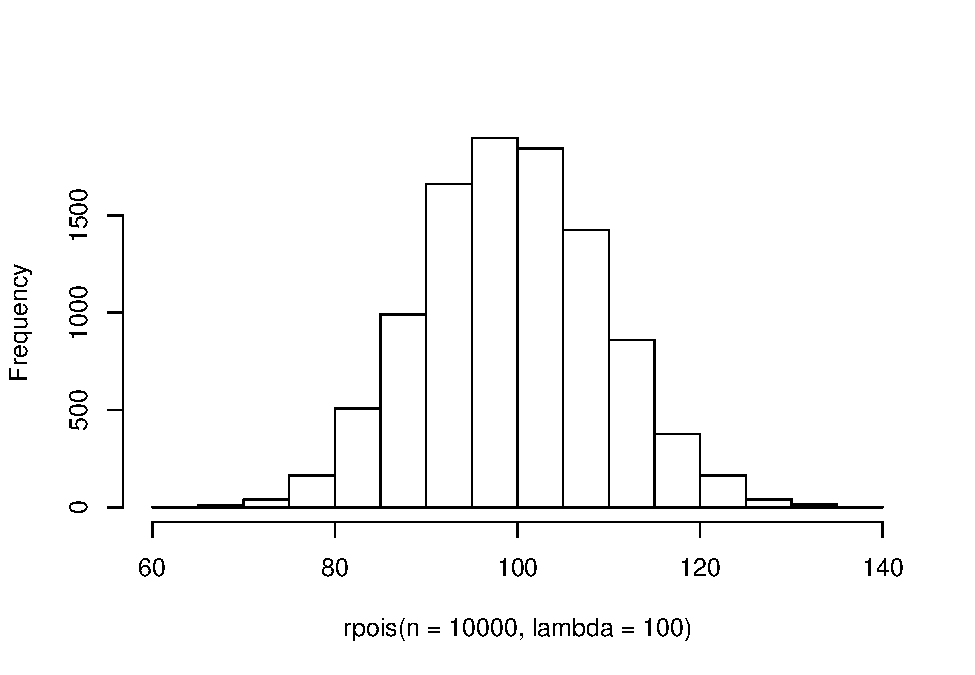
\includegraphics{worstr_files/figure-latex/unnamed-chunk-138-1.pdf}

We'll set it aside for now because it often fails us (or our data fail it, I suppose).

\hypertarget{the-negative-binomial-distribution}{%
\subsection{The negative binomial distribution}\label{the-negative-binomial-distribution}}

Okay, this one can be a little difficult to wrap your head around but it's an important one for us to know about. So, we will spend a little extra time setting this one up to try and be clear. Often, folks start out thinking that they're going to use a Poisson distribution and they end up collecting with data that do not conform to the relative inflexibility of that single-parameter distribution. Where they end up usually tends to be a negative binomial in a best case (we'll talk about challenges associated with lots of zeros later in the book).

For the purpose of this class, we are not going to dive into the mechanics of the \textbf{negative binomial distribution}, but we do need to know what it looks like and why we might need it.

One useful way to conceptualize the negative binomial is ``how long does it take for some event to occur?'' For example, we might ask how long it takes a fish to start migrating, how long it takes a sea turtle to recover in a rehabilitation center, how long it will take for a terminal patient to expire (ooh, that's dark), or how frequently we see the expression of a gene of interest. These kinds of questions are asked in aptly named ``time-to-event'' models that rely on the variance structure of the negative binomial. In the context of these kinds of questions, the negative binomial is a discrete probability distribution (and not a continuous distribution) because the ``time'' component of the distribution is actually a series of independent Bernoulli trials (holy crap!). For example: if we want to know how many days it will take for a turtle to recover from an injury, what we are really doing is asking on each day until recovery, ``Is today the day?''. Then, we flip a coin and find out. So, each day in this example is a Bernoulli trial. Another way to think about this is the number of failures occurring in a sequence before a target number of sucesses is achieved.

For the classical parameterization:

We will start by looking at how many failures are observed before one success in a sequence of Bernoulli trials.

With probability of succes equal to 0.95, it doesn't take long and most of the probability mass is near zero, with a couple of stragglers further out.

\begin{Shaded}
\begin{Highlighting}[]
\CommentTok{# Take a random sample from the negative binomial}
\NormalTok{Value <-}\StringTok{ }\KeywordTok{rnbinom}\NormalTok{(}\FloatTok{1e4}\NormalTok{, }\DataTypeTok{size=}\DecValTok{1}\NormalTok{, }\DataTypeTok{prob=}\NormalTok{.}\DecValTok{95}\NormalTok{)}

\CommentTok{# Make a histogram of it with ggplot}
\KeywordTok{ggplot}\NormalTok{() }\OperatorTok{+}\StringTok{ }\KeywordTok{geom_histogram}\NormalTok{( }\KeywordTok{aes}\NormalTok{(}\DataTypeTok{x =}\NormalTok{ Value) )}
\end{Highlighting}
\end{Shaded}

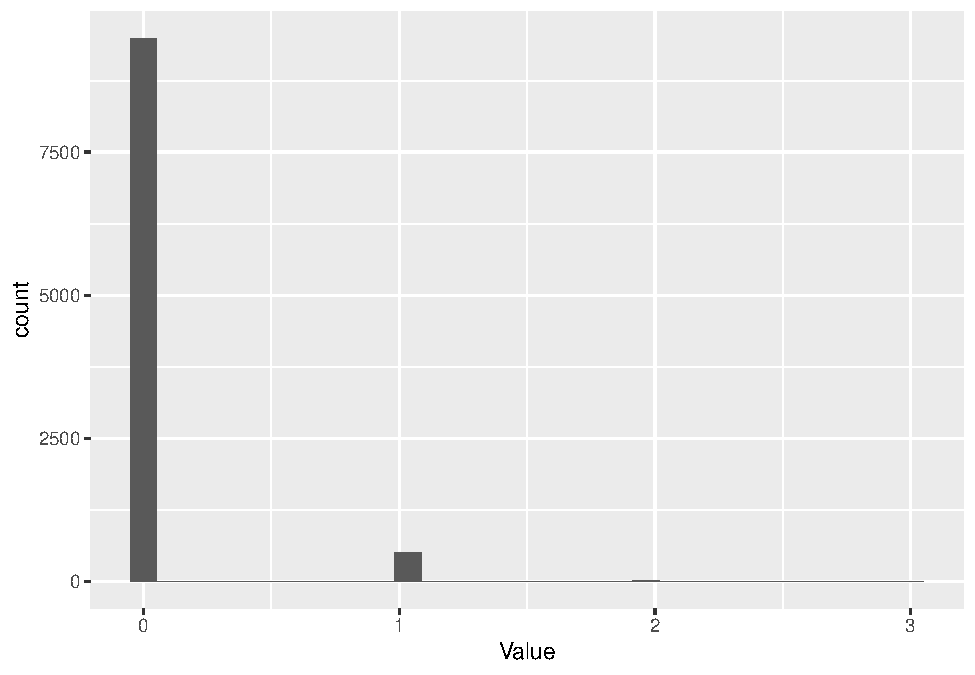
\includegraphics{worstr_files/figure-latex/unnamed-chunk-139-1.pdf}

If we decrease probability of success in each trial to 0.25, we see more failures on average before we reach success. Most of the time, it still takes less than 5 trials to reach a success, but some times it takes much longer.

\begin{Shaded}
\begin{Highlighting}[]
\CommentTok{# Take a random sample from the negative binomial}
\NormalTok{Value <-}\StringTok{ }\KeywordTok{rnbinom}\NormalTok{(}\FloatTok{1e4}\NormalTok{, }\DataTypeTok{size=}\DecValTok{1}\NormalTok{, }\DataTypeTok{prob=}\NormalTok{.}\DecValTok{25}\NormalTok{)}

\CommentTok{# Make a histogram of it with ggplot}
\KeywordTok{ggplot}\NormalTok{() }\OperatorTok{+}\StringTok{ }\KeywordTok{geom_histogram}\NormalTok{( }\KeywordTok{aes}\NormalTok{(}\DataTypeTok{x =}\NormalTok{ Value) )}
\end{Highlighting}
\end{Shaded}

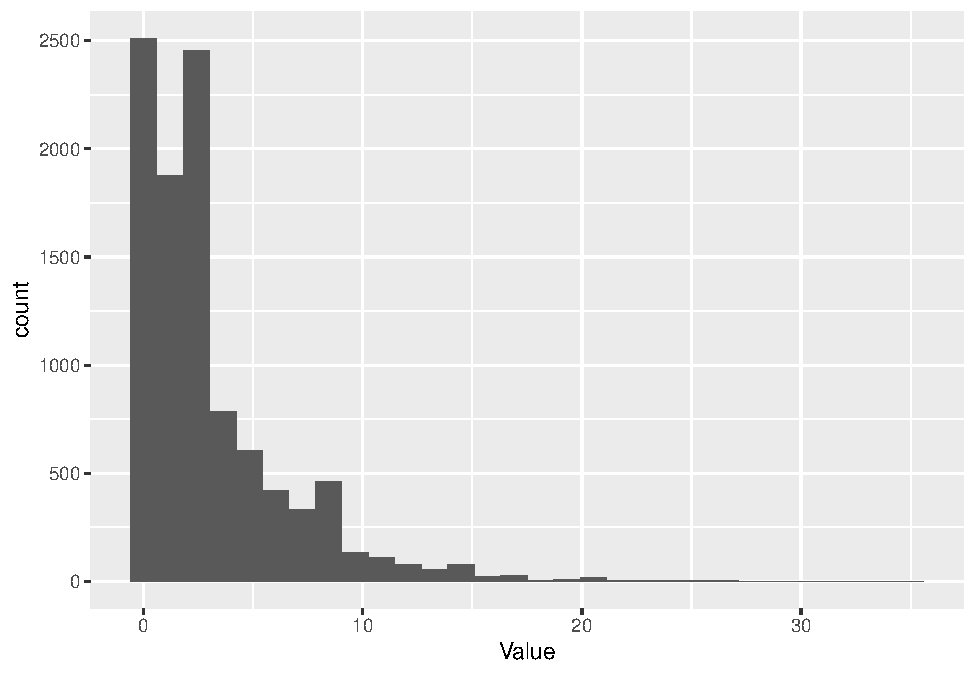
\includegraphics{worstr_files/figure-latex/unnamed-chunk-140-1.pdf}

And, if we increase the number of successes that we use for our criterion, or target, then it spreads the distribution out even further.

\begin{Shaded}
\begin{Highlighting}[]
\CommentTok{# Take a random sample from the negative binomial}
\NormalTok{Value <-}\StringTok{ }\KeywordTok{rnbinom}\NormalTok{(}\FloatTok{1e4}\NormalTok{, }\DataTypeTok{size=}\DecValTok{10}\NormalTok{, }\DataTypeTok{prob=}\NormalTok{.}\DecValTok{25}\NormalTok{)}

\CommentTok{# Make a histogram of it with ggplot}
\KeywordTok{ggplot}\NormalTok{() }\OperatorTok{+}\StringTok{ }\KeywordTok{geom_histogram}\NormalTok{( }\KeywordTok{aes}\NormalTok{(}\DataTypeTok{x =}\NormalTok{ Value) )}
\end{Highlighting}
\end{Shaded}

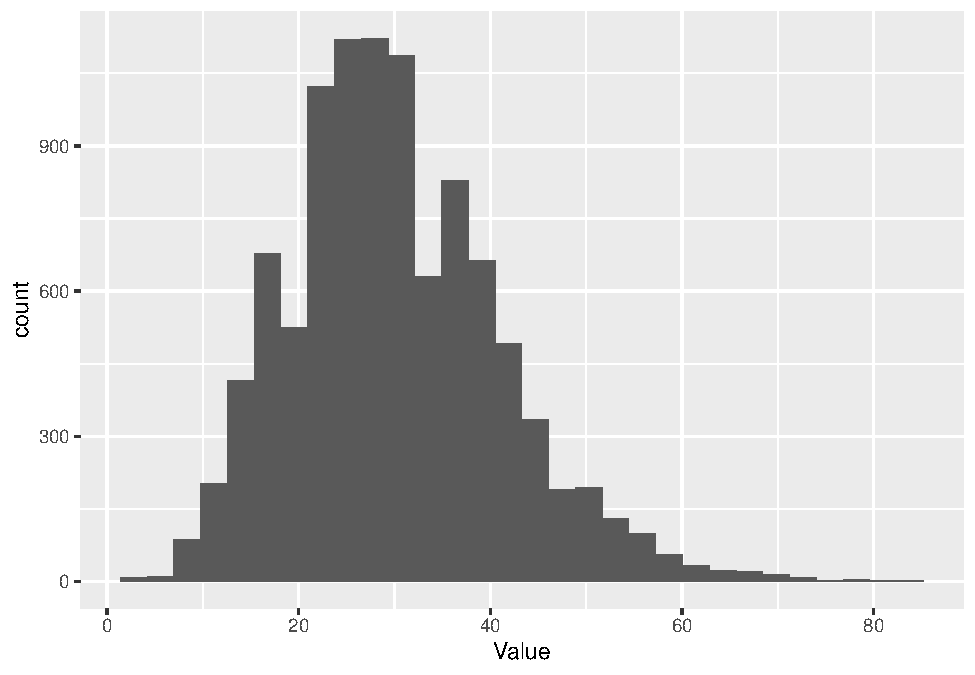
\includegraphics{worstr_files/figure-latex/unnamed-chunk-141-1.pdf}

Now, because of it's properties, the negative binomial is also useful for number of other applications that have nothing to do with interpretting the results of repeated binomial trials. Specifically, it has been widely used to represent Poisson-like processes in which the mean and variance are not equal (e.g., \textbf{overdispersion}). This has seen a lot of application in the field of ecology, especially for overdispersed count data.

Here, we draw 10,000 random samples from a negative binomial distribution with a mean of 10 and an overdispersion parameter of 1. The overdispersion parameter is called `size' because this is an alternative parameterization that is just making use of the relationships between existing parameters of the negative binomial. It's easy to grasp how the mean changes the location of the distribution.

\begin{Shaded}
\begin{Highlighting}[]
\CommentTok{# Take a random sample from the negative binomial}
\NormalTok{Value <-}\StringTok{ }\KeywordTok{rnbinom}\NormalTok{(}\FloatTok{1e4}\NormalTok{, }\DataTypeTok{mu =} \DecValTok{10}\NormalTok{, }\DataTypeTok{size =} \DecValTok{1}\NormalTok{)}

\CommentTok{# Make a histogram of it with ggplot}
\KeywordTok{ggplot}\NormalTok{() }\OperatorTok{+}\StringTok{ }\KeywordTok{geom_histogram}\NormalTok{( }\KeywordTok{aes}\NormalTok{(}\DataTypeTok{x =}\NormalTok{ Value), }\DataTypeTok{bins =} \DecValTok{20}\NormalTok{ )}
\end{Highlighting}
\end{Shaded}

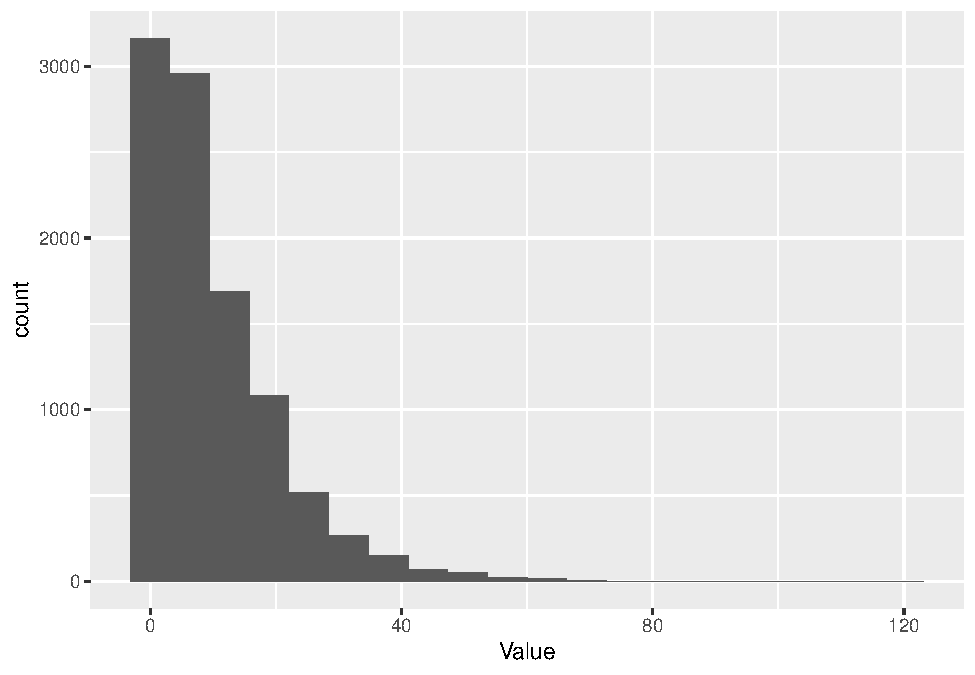
\includegraphics{worstr_files/figure-latex/unnamed-chunk-142-1.pdf}

But, note how the overdispersion parameter changes things if you run the following code:

\begin{Shaded}
\begin{Highlighting}[]
\CommentTok{# Take a random sample from the negative binomial}
\NormalTok{Value <-}\StringTok{ }\KeywordTok{rnbinom}\NormalTok{(}\FloatTok{1e4}\NormalTok{, }\DataTypeTok{mu =} \DecValTok{10}\NormalTok{, }\DataTypeTok{size =} \DecValTok{1000}\NormalTok{)}

\CommentTok{# Make a histogram of it with ggplot}
\KeywordTok{ggplot}\NormalTok{() }\OperatorTok{+}\StringTok{ }\KeywordTok{geom_histogram}\NormalTok{( }\KeywordTok{aes}\NormalTok{(}\DataTypeTok{x =}\NormalTok{ Value), }\DataTypeTok{bins =} \DecValTok{20}\NormalTok{ )}
\end{Highlighting}
\end{Shaded}

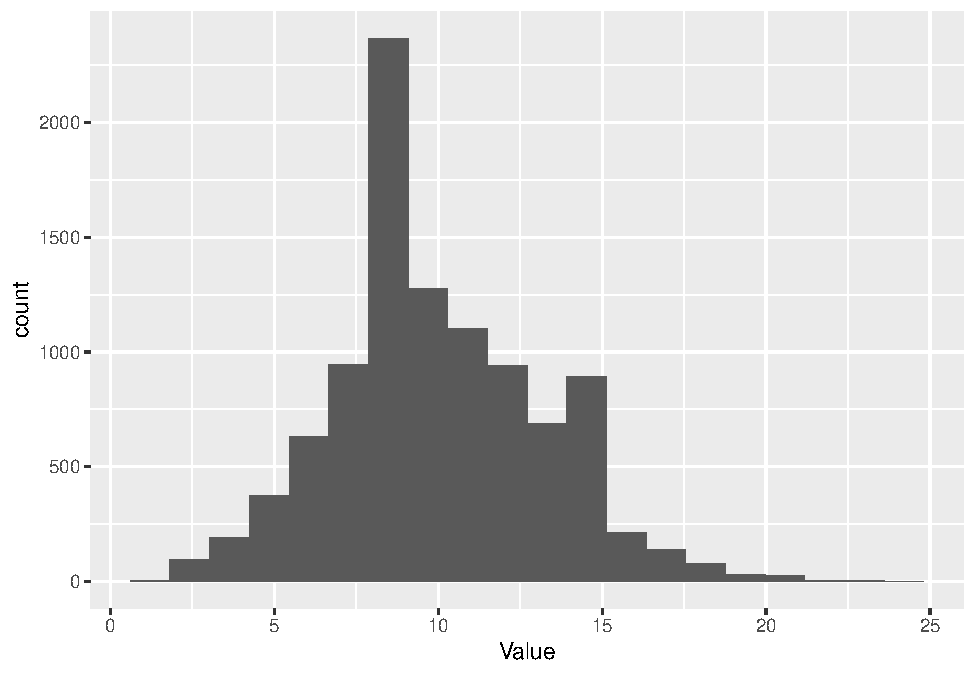
\includegraphics{worstr_files/figure-latex/unnamed-chunk-143-1.pdf}

A more intuitive way (I think) to work with the negative binomial in R is by using the \texttt{MASS} package. In this parameterization, we use the mean and the
dispersion parameter explicitly so it makes more sense:

\begin{Shaded}
\begin{Highlighting}[]
\CommentTok{# Take a random sample from the negative binomial}
\NormalTok{Value <-}\StringTok{ }\KeywordTok{rnegbin}\NormalTok{(}\FloatTok{1e4}\NormalTok{, }\DataTypeTok{mu =} \DecValTok{10}\NormalTok{, }\DataTypeTok{theta =} \DecValTok{1000}\NormalTok{)}

\CommentTok{# Make a histogram of it with ggplot}
\KeywordTok{ggplot}\NormalTok{() }\OperatorTok{+}\StringTok{ }\KeywordTok{geom_histogram}\NormalTok{( }\KeywordTok{aes}\NormalTok{(}\DataTypeTok{x =}\NormalTok{ Value), }\DataTypeTok{bins =} \DecValTok{20}\NormalTok{ )}
\end{Highlighting}
\end{Shaded}

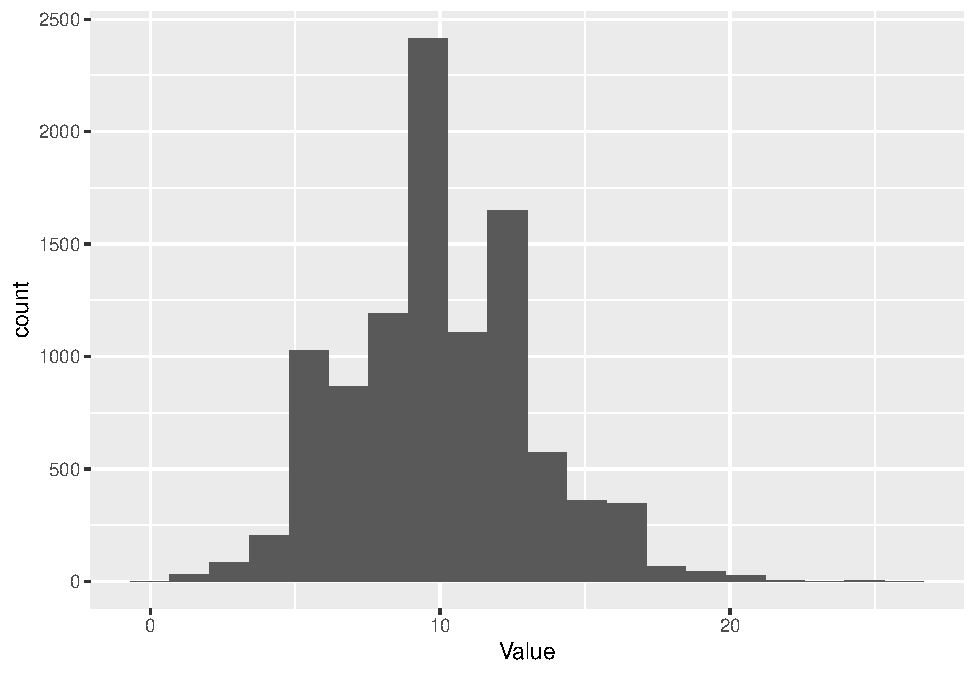
\includegraphics{worstr_files/figure-latex/unnamed-chunk-144-1.pdf}

The results are pretty much identical. Just two different naming systems for the parameters.

\hypertarget{sample-statistics}{%
\section{Sample statistics}\label{sample-statistics}}

In this section, we will learn how to derive the parameters of the \textbf{normal distribution} using a few different methods in R. We will use this opportunity to re-introduce the parameters as \textbf{moments} of the distribution so we can talk about what we mean by \textbf{confidence intervals}. We also will introduce a couple of different methods for calculating moments of a distribution. Specifically, we will look at how to derive\ldots{}

\hypertarget{moments-about-the-mean}{%
\subsection{Moments about the mean}\label{moments-about-the-mean}}

Sounds fancy, huh? Here they are, like a bandaid:

\begin{enumerate}
\def\labelenumi{\arabic{enumi}.}
\tightlist
\item
  Zeroth moment

  \begin{itemize}
  \tightlist
  \item
    This is the sum of the total probability of the distribution 1.00, always
  \end{itemize}
\item
  First moment

  \begin{itemize}
  \tightlist
  \item
    The mean
  \item
    We will look at a few ways to calculate this
  \end{itemize}
\item
  Second moment

  \begin{itemize}
  \tightlist
  \item
    The variance
  \item
    As with the mean, we will examine a couple of options for calculating
  \end{itemize}
\item
  Third moment

  \begin{itemize}
  \tightlist
  \item
    Skew
  \item
    We won't calculate for this class, but we have discussed, and this
    parameter contributes to the location/spread of the distribution (how
    far left or right the peak is)
  \end{itemize}
\item
  Fourth moment

  \begin{itemize}
  \tightlist
  \item
    Kurtosis
  \item
    Similarly, we won't cover the calculation, but this is another moment
    that we may have discussed with respect to departure from a z\\
    distribution in the normal
  \end{itemize}
\end{enumerate}

\hypertarget{estimating-parameters-of-the-normal-distribution-from-a-sample}{%
\subsection{Estimating parameters of the normal distribution from a sample}\label{estimating-parameters-of-the-normal-distribution-from-a-sample}}

The tools demonstrated below can be used for most of the probability distributions that have been implemented in R, and we could go on and on forever about them. But, for the sake of our collective sanity we will walk through the tools available using the normal distribution alone. Most of the time this will suffice because our objective in understanding other distributions is really just so that we can use them to assume asymptotic normality in response variables (with transformations) or parameter distributions (with link functions) later on anyway.

\hypertarget{method-of-moments-estimator}{%
\subsubsection{Method of moments estimator}\label{method-of-moments-estimator}}

The moments of the normal distribution are well defined, and you are probably familiar with how to calculate a mean (average) already. See if you can rearrange this in a way that makes sense with how you know to calculate a \textbf{mean} and a \textbf{variance}!

Start by simulating a variable with a known mean and standard deviation. We'll pretend that we are simulating cold temperatures here:

\begin{Shaded}
\begin{Highlighting}[]
\CommentTok{# Take a random sample from a normal}
\CommentTok{# with a mean of 20 and a standard}
\CommentTok{# deviation of 2}
\NormalTok{test_norm <-}\StringTok{ }\KeywordTok{rnorm}\NormalTok{(}\FloatTok{1e4}\NormalTok{, }\DecValTok{20}\NormalTok{, }\DecValTok{2}\NormalTok{)}
\end{Highlighting}
\end{Shaded}

First, we'll estimate it by making our own function:

\begin{Shaded}
\begin{Highlighting}[]
\CommentTok{# Write the function}
\CommentTok{# First, define a function by name}
\NormalTok{norm.mom =}\StringTok{ }\ControlFlowTok{function}\NormalTok{(x)\{      }
  
  \CommentTok{# Calculate mean}
\NormalTok{  x_bar =}\StringTok{ }\NormalTok{(}\DecValTok{1}\OperatorTok{/}\KeywordTok{length}\NormalTok{(x)) }\OperatorTok{*}\StringTok{ }\KeywordTok{sum}\NormalTok{(x) }
  
  \CommentTok{# Calculate variance}
\NormalTok{  sigma2 =}\StringTok{ }\NormalTok{(}\DecValTok{1}\OperatorTok{/}\KeywordTok{length}\NormalTok{(x)) }\OperatorTok{*}\StringTok{ }\KeywordTok{sum}\NormalTok{((x}\OperatorTok{-}\NormalTok{x_bar)}\OperatorTok{^}\DecValTok{2}\NormalTok{)}
  
  \CommentTok{# Return the calculations}
  \KeywordTok{return}\NormalTok{(}\KeywordTok{c}\NormalTok{(x_bar, sigma2))      }
  
\NormalTok{\}}
\CommentTok{# Test the function}
\KeywordTok{norm.mom}\NormalTok{(test_norm)}
\end{Highlighting}
\end{Shaded}

\begin{verbatim}
## [1] 19.97631  4.07563
\end{verbatim}

Because this one is so common, R has built-in estimators that rely on
the exact solution provided by the formulas for the first two moments
of the normal distribution:

\begin{Shaded}
\begin{Highlighting}[]
\KeywordTok{mean}\NormalTok{(test_norm)}
\end{Highlighting}
\end{Shaded}

\begin{verbatim}
## [1] 19.97631
\end{verbatim}

\begin{Shaded}
\begin{Highlighting}[]
\KeywordTok{var}\NormalTok{(test_norm)}
\end{Highlighting}
\end{Shaded}

\begin{verbatim}
## [1] 4.076038
\end{verbatim}

Wow, that was a lot less code. That is the beauty of having these functions available. How do these compare to the answers returned by our function if you scroll back up?

\hypertarget{maximum-likelihood-estimator}{%
\subsubsection{Maximum likelihood estimator}\label{maximum-likelihood-estimator}}

R also has built-in \textbf{maximum likelihood} estimators that provide an exact solution to the first two moments of the normal distribution. These are available through the \texttt{MASS} package.

\begin{Shaded}
\begin{Highlighting}[]
\KeywordTok{fitdistr}\NormalTok{(test_norm, }\StringTok{'normal'}\NormalTok{)}
\end{Highlighting}
\end{Shaded}

\begin{verbatim}
##       mean           sd     
##   19.97631239    2.01881895 
##  ( 0.02018819) ( 0.01427521)
\end{verbatim}

Only one problem here: R doesn't report the second moment! It reports
the square root of the second moment: the \textbf{standard deviation}!

Finally, let's write our own function and maximize the likelihood with the \texttt{optim()} function in R.

\begin{Shaded}
\begin{Highlighting}[]
\CommentTok{# Define the function}
\NormalTok{normal.lik =}\StringTok{ }\ControlFlowTok{function}\NormalTok{(theta, y)\{}
  
  \CommentTok{# The starting value for}
  \CommentTok{# mu that we provide}
\NormalTok{  mu =}\StringTok{ }\NormalTok{theta[}\DecValTok{1}\NormalTok{]}
  
  \CommentTok{# The starting value for}
  \CommentTok{# sigma2 that we provide}
\NormalTok{  sigma2 =}\StringTok{ }\NormalTok{theta[}\DecValTok{2}\NormalTok{]}
  
  \CommentTok{# Number of observations in the data}
\NormalTok{  n =}\StringTok{ }\KeywordTok{nrow}\NormalTok{(y)}
  
  \CommentTok{# Compute the log likelihood of the}
  \CommentTok{# data (y) using the likelihood}
  \CommentTok{# function for the normal distribution}
  \CommentTok{# given the starting values for our}
  \CommentTok{# parameters (contained in the vector 'theta')}
\NormalTok{  logl =}\StringTok{ }\FloatTok{-.5}\OperatorTok{*}\NormalTok{n}\OperatorTok{*}\KeywordTok{log}\NormalTok{(}\DecValTok{2}\OperatorTok{*}\NormalTok{pi) }\FloatTok{-.5}\OperatorTok{*}\NormalTok{n}\OperatorTok{*}\KeywordTok{log}\NormalTok{(sigma2)}\OperatorTok{-}\NormalTok{(}\DecValTok{1}\OperatorTok{/}\NormalTok{(}\DecValTok{2}\OperatorTok{*}\NormalTok{sigma2))}\OperatorTok{*}\KeywordTok{sum}\NormalTok{((y}\OperatorTok{-}\NormalTok{mu)}\OperatorTok{**}\DecValTok{2}\NormalTok{)}
  \KeywordTok{return}\NormalTok{(}\OperatorTok{-}\NormalTok{logl)}
\NormalTok{\}}
\end{Highlighting}
\end{Shaded}

Now, we use the \texttt{optim} function to maximize the likelihood of the data
(technically by minimizing the -2*log{[}likehood{]}) given different values of
our parameters (\texttt{mu} and \texttt{sigma2}).

To get started, we need to take a guess at what those parameters could be. (Yes, we know they are mu = 20 and sd = 2)

\begin{Shaded}
\begin{Highlighting}[]
\KeywordTok{optim}\NormalTok{(}\KeywordTok{c}\NormalTok{(}\DecValTok{20}\NormalTok{, }\DecValTok{4}\NormalTok{), normal.lik, }\DataTypeTok{y=}\KeywordTok{data.frame}\NormalTok{(test_norm))}
\end{Highlighting}
\end{Shaded}

\begin{verbatim}
## $par
## [1] 19.976100  4.074998
## 
## $value
## [1] 21214.51
## 
## $counts
## function gradient 
##       49       NA 
## 
## $convergence
## [1] 0
## 
## $message
## NULL
\end{verbatim}

The pieces are in \texttt{pars} here (right where we told R to put them!). We can also make the output into an object and call the parts by name:

\begin{Shaded}
\begin{Highlighting}[]
\CommentTok{# Make it into an object}
\NormalTok{est =}\StringTok{ }\KeywordTok{optim}\NormalTok{(}\KeywordTok{c}\NormalTok{(}\DecValTok{0}\NormalTok{, }\DecValTok{1}\NormalTok{),}
\NormalTok{            normal.lik,}
            \DataTypeTok{y=}\KeywordTok{data.frame}\NormalTok{(test_norm)}
\NormalTok{            ) }
\end{Highlighting}
\end{Shaded}

\begin{verbatim}
## Warning in log(sigma2): NaNs produced

## Warning in log(sigma2): NaNs produced

## Warning in log(sigma2): NaNs produced

## Warning in log(sigma2): NaNs produced

## Warning in log(sigma2): NaNs produced

## Warning in log(sigma2): NaNs produced
\end{verbatim}

Look at the structure I'll be damned, it's a list! Hey, we learned about those!

\begin{Shaded}
\begin{Highlighting}[]
\KeywordTok{str}\NormalTok{(est)   }
\end{Highlighting}
\end{Shaded}

\begin{verbatim}
## List of 5
##  $ par        : num [1:2] 19.98 4.07
##  $ value      : num 21215
##  $ counts     : Named int [1:2] 99 NA
##   ..- attr(*, "names")= chr [1:2] "function" "gradient"
##  $ convergence: int 0
##  $ message    : NULL
\end{verbatim}

And, here are the estimates:

\begin{Shaded}
\begin{Highlighting}[]
\CommentTok{# Both}
\NormalTok{est}\OperatorTok{$}\NormalTok{par }
\end{Highlighting}
\end{Shaded}

\begin{verbatim}
## [1] 19.975793  4.071458
\end{verbatim}

\begin{Shaded}
\begin{Highlighting}[]
\CommentTok{# The mean  }
\NormalTok{est}\OperatorTok{$}\NormalTok{par[}\DecValTok{1}\NormalTok{]}
\end{Highlighting}
\end{Shaded}

\begin{verbatim}
## [1] 19.97579
\end{verbatim}

\begin{Shaded}
\begin{Highlighting}[]
\CommentTok{# The variance  }
\NormalTok{est}\OperatorTok{$}\NormalTok{par[}\DecValTok{2}\NormalTok{] }
\end{Highlighting}
\end{Shaded}

\begin{verbatim}
## [1] 4.071458
\end{verbatim}

There you have it, a couple of different ways to calculate parameters of the normal distribution using a couple of different approaches each.

\hypertarget{quantiles-and-other-descriptive-statistics}{%
\subsection{Quantiles and other descriptive statistics}\label{quantiles-and-other-descriptive-statistics}}

There are a number of other ways we might like to describe this this (or any) sampling distribution. Here are a few examples that we will work with this semester.

\begin{Shaded}
\begin{Highlighting}[]
\CommentTok{# Here is the median, or 50th percentile}
\KeywordTok{median}\NormalTok{(test_norm) }
\end{Highlighting}
\end{Shaded}

\begin{verbatim}
## [1] 19.96641
\end{verbatim}

\begin{Shaded}
\begin{Highlighting}[]
\CommentTok{# The 95% confidence limits}
\KeywordTok{quantile}\NormalTok{(test_norm, }\DataTypeTok{probs =} \KeywordTok{c}\NormalTok{(}\FloatTok{0.025}\NormalTok{, }\FloatTok{0.975}\NormalTok{)) }
\end{Highlighting}
\end{Shaded}

\begin{verbatim}
##     2.5%    97.5% 
## 16.06509 23.95483
\end{verbatim}

\begin{Shaded}
\begin{Highlighting}[]
\CommentTok{# Interquartile range (Q1 and Q3)}
\KeywordTok{quantile}\NormalTok{(test_norm, }\DataTypeTok{probs =} \KeywordTok{c}\NormalTok{(}\FloatTok{0.25}\NormalTok{, }\FloatTok{0.75}\NormalTok{))    }
\end{Highlighting}
\end{Shaded}

\begin{verbatim}
##      25%      75% 
## 18.60817 21.31751
\end{verbatim}

\begin{Shaded}
\begin{Highlighting}[]
\CommentTok{# Range of sample}
\KeywordTok{range}\NormalTok{(test_norm)                             }
\end{Highlighting}
\end{Shaded}

\begin{verbatim}
## [1] 11.68006 28.63840
\end{verbatim}

\hypertarget{next5}{%
\section{Next steps}\label{next5}}

Here, we have explored some of the probability distributions that we use to describe samples (data) that we collect from the real world. In \protect\hyperlink{Chapter6}{Chapter 6} we will explore how these sampling distributions can be used for statistical inference before diving into applied statistical analyses for the remainder of the book. Hopefully the order of things is starting to make some sense! If not, well\ldots this \emph{is} The Worst Stats Text eveR.

\hypertarget{Chapter6}{%
\chapter{Inferential statistics}\label{Chapter6}}

These are hot peppers. Like hot peppers, statistics can cause pain and heartburn if you are not accustomed to them. Ready or not, let's get munching!!

This week we will begin conducting our first statistical tests! We are going to start small and simple, and we will build complexity during the remainder of the semester. We will also start to make more use of some of the programming techniques that you have been developing, and we will build a foundation for moving into regression models in coming weeks.

We'll start with some simple methods for testing hypotheses about sampling distributions this week. Although relatively limited in scope within the fields of biology and ecology, these tend to be fairly robust tests, and can be powerful tools if studies are designed thoughtfully. For this week, we will focus on implementation of one-sample t-tests, two-sample t-tests, Wilcox tests, and frequency analysis using a \(\chi^2\) test. Within the context of the assumptions of these tests we will also discuss the F-test and the Shapiro-Wilk test of normality. In short, you probably will learn more statistical tests in this preliminary chapter about statistical inference than you have in your college career to this point. Take your time and soak in all the mathy goodness. We'll need it!

For this Chapter, we will continue working with packages from the \texttt{tidyverse}. You can go ahead and put this in the top of your code for the chapter if you want to load it all at once:

\begin{Shaded}
\begin{Highlighting}[]
\KeywordTok{library}\NormalTok{(tidyverse)}
\end{Highlighting}
\end{Shaded}

We will also need the grass carp data for this exercise, which we will load from \texttt{grasscarp.csv}. Remember that you can download all of the class data here or you can get the individual \texttt{grasscarp.csv} file by clicking here and saving with \texttt{Ctrl\ +\ S} (Windows) or \texttt{Command\ +\ S} (Mac OS-X).

These data come from a long-term study of fish population responses to changes in their primary food source, the invasive hydrilla (\emph{Hydrilla verticallata}). There are a whole bunch of columns in here! The important variables for this chapter are \texttt{Year} (year of fish collection), \texttt{Age} (the age of each fish), \texttt{Length} (total length of fish in mm), and \texttt{hydrilla} (hectares of hydrilla measured each \texttt{Year}).

\hypertarget{one-sample-tests}{%
\section{One-sample tests}\label{one-sample-tests}}

Sometimes, we are interested in simply knowing whether or not the measurements we've obtained from an individual or a group are representative of a larger population. For example, we may have a `control' group in an experiment and we want to know if the group is truly representative of the population average or some measurement we have collected from a different biological population. For these situations, we will rely on one-sample tests this week and we'll look at other (totally related) options moving forward.

\hypertarget{one-sample-t-test}{%
\subsection{One sample t-test}\label{one-sample-t-test}}

We will examine parametric and non-parametric examples of one-sample tests here to demonstrate why and how we use them.

Let's start with a simple example of how we might do this, and what the results actually mean. We'll use some data from grass carp (\emph{Ctenopharyngodon idella}) from Lake Gaston, Virginia and North Carolina, USA for this example. We will compare the size of grass carp at specific ages with their population density using a few different tools

Read in the data set:

\begin{Shaded}
\begin{Highlighting}[]
\NormalTok{  grasscarp <-}\StringTok{ }\KeywordTok{read.csv}\NormalTok{(}\StringTok{'data/grasscarp.csv'}\NormalTok{)}
\end{Highlighting}
\end{Shaded}

Just for funsies, you could also read this in directly from the link to the raw data in the \href{https://github.com/danStich/worst-r/tree/master/data}{GitHub repository for this book} if you have an internet connection:

\begin{Shaded}
\begin{Highlighting}[]
\NormalTok{grasscarp <-}\StringTok{ }\KeywordTok{read.csv}\NormalTok{(}\StringTok{'https://raw.githubusercontent.com/danStich/worst-r/master/data/grasscarp.csv'}\NormalTok{)}
\end{Highlighting}
\end{Shaded}

Remember to check out the data set in your Environment tab so you understand how many observations there are and how many variables (as well as their types).

Let's start by asking a simple biological question: is the size of age-3 grass carp different from the average size of fish in this population?

First, let's create a sample that includes only age-3 fish. We will store this to a new vector called \texttt{age3\_lengths}.

\begin{Shaded}
\begin{Highlighting}[]
\NormalTok{age3_lengths <-}\StringTok{ }\NormalTok{grasscarp}\OperatorTok{$}\NormalTok{Length[grasscarp}\OperatorTok{$}\NormalTok{Age }\OperatorTok{==}\StringTok{ }\DecValTok{3}\NormalTok{]}
\end{Highlighting}
\end{Shaded}

Now, let's compare the \texttt{Length} of age-3 fish to the rest of the population using a one-sample t-test. To do this, we need to pass \texttt{age3\_lengths}

\begin{Shaded}
\begin{Highlighting}[]
\CommentTok{# Run the test and save the output to an object}
\NormalTok{our_test =}\StringTok{ }\KeywordTok{t.test}\NormalTok{(age3_lengths,}
                  \DataTypeTok{mu =} \KeywordTok{mean}\NormalTok{(grasscarp}\OperatorTok{$}\NormalTok{Length),}
                  \DataTypeTok{conf.level =} \FloatTok{0.95}
\NormalTok{                  )}

\CommentTok{# Print the results of the object to the console}
\KeywordTok{print}\NormalTok{(our_test)}
\end{Highlighting}
\end{Shaded}

\begin{verbatim}
## 
## 	One Sample t-test
## 
## data:  age3_lengths
## t = -18.829, df = 47, p-value < 2.2e-16
## alternative hypothesis: true mean is not equal to 973.0118
## 95 percent confidence interval:
##  749.2547 792.4536
## sample estimates:
## mean of x 
##  770.8542
\end{verbatim}

Okay, so what does that mean???

\begin{quote}
First, let's look at what we've done here.
\end{quote}

We've conducted a one-sample t-test.

The null hypothesis was that:

\begin{quote}
(H\textsubscript{0}): the sample (age-3 fish) did not differ in \texttt{Length} from the mean of the population.
\end{quote}

This is because we stated no specific alternative hypothesis when we executed the t-test above. If we had used a different alternative hypothesis (i.e.~\texttt{greater} or \texttt{less} in the argument \texttt{alternative}) then our null would be formalized as: ``The length of age-3 fish is not significantly greater (or less) than the population mean''.

Finally, we specified the confidence level. Here, we are told R that we want to know the result with a confidence level of 95\% (0.95). This corresponds to a Type-I error rate (\(\alpha\)) of 0.05. This means we are looking for \emph{p} \textless{} 0.05 to conclude that the sample is statistically different from the population mean. Since p \textless{} 0.001, we reject the H\textsubscript{0} and conclude that age-3 fish are significantly shorter than the population mean.

\hypertarget{output}{%
\subsubsection{Output}\label{output}}

R returns the output of statistical tests as objects, and you can reference any part of those objects by name or index. The type of object that R returns, and how you access the parts depends on the type of test you ran and with what options.

Like so many other models objects, our one sample t-test is stored as a list:

\begin{Shaded}
\begin{Highlighting}[]
\KeywordTok{str}\NormalTok{(our_test)}
\end{Highlighting}
\end{Shaded}

\begin{verbatim}
## List of 10
##  $ statistic  : Named num -18.8
##   ..- attr(*, "names")= chr "t"
##  $ parameter  : Named num 47
##   ..- attr(*, "names")= chr "df"
##  $ p.value    : num 1.57e-23
##  $ conf.int   : num [1:2] 749 792
##   ..- attr(*, "conf.level")= num 0.95
##  $ estimate   : Named num 771
##   ..- attr(*, "names")= chr "mean of x"
##  $ null.value : Named num 973
##   ..- attr(*, "names")= chr "mean"
##  $ stderr     : num 10.7
##  $ alternative: chr "two.sided"
##  $ method     : chr "One Sample t-test"
##  $ data.name  : chr "age3_lengths"
##  - attr(*, "class")= chr "htest"
\end{verbatim}

We can just look at the names if there are specific pieces in which we are interested. For example, we might want to save the p-value (\texttt{p.value}):

\begin{Shaded}
\begin{Highlighting}[]
\CommentTok{# Shows us the names of the things inside the model list}
  \KeywordTok{names}\NormalTok{(our_test) }
\end{Highlighting}
\end{Shaded}

\begin{verbatim}
##  [1] "statistic"   "parameter"   "p.value"     "conf.int"    "estimate"   
##  [6] "null.value"  "stderr"      "alternative" "method"      "data.name"
\end{verbatim}

\begin{Shaded}
\begin{Highlighting}[]
\CommentTok{# This stores our p-value to an object for use}
\NormalTok{  p_out =}\StringTok{ }\NormalTok{our_test}\OperatorTok{$}\NormalTok{p.value }
  
\CommentTok{# And of course we can look at it}
  \KeywordTok{print}\NormalTok{(p_out)             }
\end{Highlighting}
\end{Shaded}

\begin{verbatim}
## [1] 1.572767e-23
\end{verbatim}

Now we can go through the output as it is displayed by:

\begin{Shaded}
\begin{Highlighting}[]
\CommentTok{# Print a summary of the test}
  \KeywordTok{print}\NormalTok{(our_test)}
\end{Highlighting}
\end{Shaded}

\begin{verbatim}
## 
## 	One Sample t-test
## 
## data:  age3_lengths
## t = -18.829, df = 47, p-value < 2.2e-16
## alternative hypothesis: true mean is not equal to 973.0118
## 95 percent confidence interval:
##  749.2547 792.4536
## sample estimates:
## mean of x 
##  770.8542
\end{verbatim}

The first line of the output gives us the actual data that with which we are working- nothing of interest here other than a quick sanity check until later on in the course.

The second line shows the `statistics' that we are interested in: \texttt{t} is the calculated value of the test statistic for the t-test in this case. The \texttt{df}, or degrees of freedom, is the number of observations in the sample, minus the number of parameters that we are estimating (in this case, just one: the mean). Our \texttt{p-value} is the probability of observing data that are more extreme than what we observed if the null hypothesis is in fact true (i.e.~the probability that rejection of the null is inappropriate). Again, because it is smaller than \(\alpha\) we reject the null and accept the alternative hypothesis.

Our \texttt{alteranive\ hypothesis} (H\textsubscript{A}) was that the sample mean is not equal to population mean. We can specify other alternatives (and therefore nulls) in this and other models in R.

Finally, R reports the mean and the 95\% confidence interval of \texttt{age3\_lengths}.

\hypertarget{assumptions}{%
\subsubsection{Assumptions}\label{assumptions}}

It's always important for us to think about the assumptions that we are making when (read \emph{before}) conducting a statistical test. First, there are implicit assumptions that we make. For example, we assume that the data are representative and were collected in a random manner in this case. Then, there are explicit assumptions that we make in specific tests.

For the one-sample t-test, the assumption that we really care about is:

\begin{enumerate}
\def\labelenumi{\arabic{enumi}.}
\tightlist
\item
  The data are normally distributed
\end{enumerate}

The t-test is generally robust to violations of this assumption provided that sample sizes are large enough (Google Central Limit Theorem, this is The Worst Stats Text eveR). But, it is always good to check. In particular, when we are working with small sample sizes like this example (n = \texttt{48}), we should really make sure that things look okay.

\hypertarget{checking-assumptions}{%
\subsubsection{Checking assumptions}\label{checking-assumptions}}

Visual check for normality

One simple way to gauge assumptions of normality is to look at a plot of the data. As you will see later, we are usually concerned with the \emph{residuals}, but we can look at the actual data here because we have only one group and if it's normal so are its errors.

Have a quick look at these to see what we are working with using the histogram code from \protect\hyperlink{Chapter4}{Chapter 4}. I set the x-axis limits below using the maximum \texttt{Length} from the \texttt{grasscarp} data so we can see what part of the length range we've sampled here.

\begin{Shaded}
\begin{Highlighting}[]
\NormalTok{p <-}\StringTok{ }\KeywordTok{ggplot}\NormalTok{() }\OperatorTok{+}\StringTok{ }
\StringTok{  }\KeywordTok{geom_histogram}\NormalTok{(}\KeywordTok{aes}\NormalTok{(age3_lengths), }\DataTypeTok{bins =} \DecValTok{30}\NormalTok{) }\OperatorTok{+}\StringTok{ }
\StringTok{  }\KeywordTok{scale_x_continuous}\NormalTok{(}\DataTypeTok{limits=}\KeywordTok{c}\NormalTok{(}\DecValTok{0}\NormalTok{, }\KeywordTok{max}\NormalTok{(grasscarp}\OperatorTok{$}\NormalTok{Length)), }\DataTypeTok{expand =} \KeywordTok{c}\NormalTok{(}\DecValTok{0}\NormalTok{, }\DecValTok{0}\NormalTok{)) }\OperatorTok{+}\StringTok{ }
\StringTok{  }\KeywordTok{scale_y_continuous}\NormalTok{(}\DataTypeTok{expand =} \KeywordTok{c}\NormalTok{(}\DecValTok{0}\NormalTok{, }\DecValTok{0}\NormalTok{)) }\OperatorTok{+}\StringTok{ }
\StringTok{  }\KeywordTok{xlab}\NormalTok{(}\StringTok{"Total length (mm)"}\NormalTok{) }\OperatorTok{+}
\StringTok{  }\KeywordTok{ylab}\NormalTok{(}\StringTok{"Count"}\NormalTok{) }\OperatorTok{+}
\StringTok{  }\KeywordTok{theme_classic}\NormalTok{() }\OperatorTok{+}
\StringTok{  }\KeywordTok{theme}\NormalTok{(}
    \DataTypeTok{axis.title.x =} \KeywordTok{element_text}\NormalTok{(}\DataTypeTok{vjust =} \DecValTok{-1}\NormalTok{),}
    \DataTypeTok{axis.title.y =} \KeywordTok{element_text}\NormalTok{(}\DataTypeTok{vjust =} \DecValTok{3}\NormalTok{),}
    \DataTypeTok{panel.grid =} \KeywordTok{element_blank}\NormalTok{()}
\NormalTok{  )}
\KeywordTok{print}\NormalTok{(p)}
\end{Highlighting}
\end{Shaded}

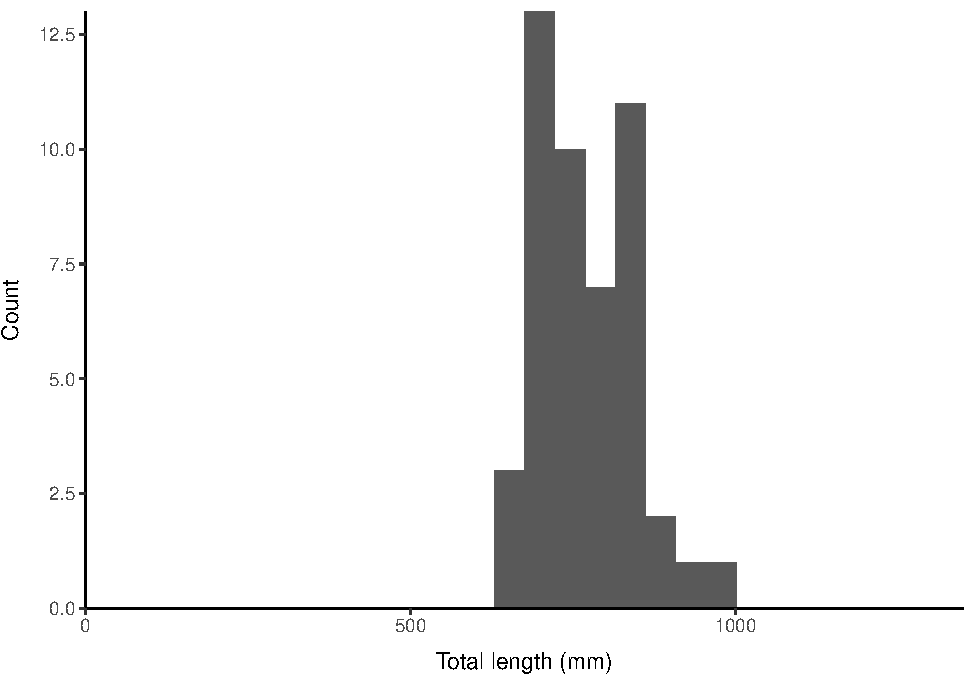
\includegraphics{worstr_files/figure-latex/unnamed-chunk-163-1.pdf}
Sure, looks totally normal to me? Wouldn't it be great if there were a statistical test for determining whether this sample is different from the normal? Great that you should ask.

\hypertarget{tests-of-normality-shapiro-wilk}{%
\paragraph{Tests of normality (Shapiro-Wilk)}\label{tests-of-normality-shapiro-wilk}}

The Shapiro-Wilk test is commonly used to test normality of a distribution as a check of assumptions. We can use this to test whether our data deviate from normal in the following manner:

\begin{Shaded}
\begin{Highlighting}[]
\KeywordTok{shapiro.test}\NormalTok{(age3_lengths)}
\end{Highlighting}
\end{Shaded}

\begin{verbatim}
## 
## 	Shapiro-Wilk normality test
## 
## data:  age3_lengths
## W = 0.95715, p-value = 0.07746
\end{verbatim}

First, note that the test statistic is the \texttt{W} statistic for this test.

Second, we have a p-value of \texttt{0.0774637}. \textbf{Oh, no}! Wait, what does that mean?

For this test, we actually don't want p \textless{} 0.05 if we are relying on assumptions of normality, so this is a ``good'' thing. But, it doesn't necessarily mean \texttt{age3\_lengths} is normally distributed. It just means that we can't tell if the sample we have collected is different from normal (we fail to reject the null but can't ``accept'' it). I guess that is good enough, but that p-value is awfully close to 0.05 for my taste.

So, are we up that proverbial tributary without a paddle, or can we salvage the mess and move on with life? Don't worry, there's a statistical test for that, too.

\hypertarget{wilcox-test}{%
\subsection{Wilcox test}\label{wilcox-test}}

You can think of the Wilcox test as a non-parametric analog of the t-test. In general, non-parametric tests tend to be slightly more ``conservative'' than the parametric alternatives because they require fewer assumptions. However, non-parametric tests can be useful where our data are not normal, or we don't feel we have sufficient data to know (hmm\ldots maybe don't conduct any tests, in that case!).

Here, we are checking for shifts in the median (not the mean) of one or more samples.

Why is this? The mean of a non-normal distribution is not always a useful descriptor of the probability mass under a distribution (it still describes `central tendency' but does not necessarily describe the place where `most of the data are'). But, the median always (as in always, always, always) describes central tendency of the data, so we can pretty much use it for describing any sample. This is because the median is defined as the ``middle'' value. That is, half of the data should fall on either side of the median if you lined up all of your data on the equator (wrong metaphor?).

\ldots back to the Wilcox test.

\begin{Shaded}
\begin{Highlighting}[]
\CommentTok{# First, do this and have a quick read:}
\NormalTok{  ?wilcox.test}
\end{Highlighting}
\end{Shaded}

Now we can actually run a test to see if the median length of age-3 fish is statistically different from the median value of length in the sample.

\begin{Shaded}
\begin{Highlighting}[]
    \KeywordTok{wilcox.test}\NormalTok{(}
\NormalTok{      age3_lengths,}
      \DataTypeTok{mu =} \KeywordTok{median}\NormalTok{(grasscarp}\OperatorTok{$}\NormalTok{Length),}
      \DataTypeTok{alternative =} \StringTok{'less'}\NormalTok{,    }\CommentTok{# Note different alternative here!}
      \DataTypeTok{exact =} \OtherTok{FALSE}            \CommentTok{# Not much data, so not exact}
\NormalTok{    )}
\end{Highlighting}
\end{Shaded}

\begin{verbatim}
## 
## 	Wilcoxon signed rank test with continuity correction
## 
## data:  age3_lengths
## V = 0, p-value = 8.414e-10
## alternative hypothesis: true location is less than 1007
\end{verbatim}

Interpretting the results is essentially the same as for the t-test, but without the degrees of freedom, so we won't belabor this. Importantly, the test, being robust to any distributional assumptions, should also (and does) tell us that the length of age-3 fish is significantly shorter than the population mean (or median- whichever you used).

\hypertarget{two-sample-tests}{%
\section{Two-sample tests}\label{two-sample-tests}}

Okay, with that out of the way, now we can get on to some tests that might be a little more meaningful to most people. We can use \textbf{two-sample} tests to whether two groups differ in some metric of interest. This lends itself naturally to use in controlled experiments that we conduct in laboratories, for example.

\hypertarget{the-two-sample-t-test}{%
\subsection{The two-sample t-test}\label{the-two-sample-t-test}}

If you have been exposed to only one statistical test already it is probably the two-sample t-test. This is a test that is used to test for differences in some continuous variable between two groups. The test statistic itself is pretty trivial to calculate. You can find a video of that \href{https://www.khanacademy.org/math/ap-statistics/two-sample-inference/two-sample-t-test-means/v/two-sample-t-test-for-difference-of-means}{here}. \textbf{Seriously, if you have never done a t-test, watch the 6-minute video now}. Otherwise, you may not understand what follows. I am not going to go into the math here because this is The Worst Stats Text eveR. The video will also help you understand how ANOVA and other tests work later. Understanding how these tests work will give you phenomenal cosmic powers when it comes to analyzing biological data. If you email asking me how a t-test works, I am going to send you this video.

Let's keep working with the \texttt{grasscarp} data for now for the sake of consistency. But, now we want to know if there is a difference in mean length of fish depending on whether their population density is high or low. To look at this, we'll need to make some groups in our \texttt{grasscarp} data that correspond to years of high and low density.

You can compare fish density between years quickly using the summary pipeline demonstrated in \protect\hyperlink{Chapter3}{Chapter 3}

\begin{Shaded}
\begin{Highlighting}[]
\NormalTok{grasscarp }\OperatorTok
\StringTok{  }\KeywordTok{group_by}\NormalTok{(Year) }\OperatorTok
\StringTok{  }\KeywordTok{summarize}\NormalTok{(}\DataTypeTok{dens =} \KeywordTok{unique}\NormalTok{(nha))}
\end{Highlighting}
\end{Shaded}

\begin{verbatim}
## # A tibble: 5 x 2
##    Year  dens
##   <int> <int>
## 1  2006    21
## 2  2007    58
## 3  2009    44
## 4  2010    43
## 5  2017   127
\end{verbatim}

You can see that density was much higher in \texttt{2017} than in any of the preceding years. This is because hydrilla area was reduced by several hundred hectares (\texttt{ha}) between 2010 and 2014 (which was actually the reason we went out to collect more data in 2017). But, these are just means and we need to be able to account for the variability in these measurements to call it science.

So, let's build some groups based on high and low density years. First, we'll add a new categorical variable to \texttt{grasscarp} called ``\texttt{density}'', and we'll fill it all in with the word \texttt{"low"} because there is only one year when density was high.

\begin{Shaded}
\begin{Highlighting}[]
\NormalTok{grasscarp}\OperatorTok{$}\NormalTok{density <-}\StringTok{ "low"}
\end{Highlighting}
\end{Shaded}

Next, we'll change all of the observations for 2017 to \texttt{"high"} so we have low density and high density groupings in our \texttt{density} column. This way, we only have to change the variable for one year.

\begin{Shaded}
\begin{Highlighting}[]
\NormalTok{grasscarp}\OperatorTok{$}\NormalTok{density[grasscarp}\OperatorTok{$}\NormalTok{Year }\OperatorTok{==}\StringTok{ }\DecValTok{2017}\NormalTok{] <-}\StringTok{ "high"}
\end{Highlighting}
\end{Shaded}

Then, we'll subset the data to look at a single age so our comparisons are fair between years. I picked \texttt{Age\ ==\ 10} because 10 years is in the middle of the range of ages in the data set. You can try it with another age as long as there are enough data.

\begin{Shaded}
\begin{Highlighting}[]
\NormalTok{mid_carps <-}\StringTok{ }\NormalTok{grasscarp }\OperatorTok\StringTok{ }\KeywordTok{subset}\NormalTok{(Age }\OperatorTok{==}\StringTok{ }\DecValTok{10}\NormalTok{)}
\end{Highlighting}
\end{Shaded}

Now, we can conduct our two-sample t-test!

The syntax is pretty straightforward, and is similar to what we used above, except that now we have two groups so we will omit \texttt{mu} and specify the t-test as a formula with independent (x, \texttt{density}) and dependent (y, \texttt{Length}) variables. There is no pairing of our observations, so we specify \texttt{paired\ =\ FALSE}, and we tell R we don't want to assume that the variance of \texttt{Length} is equal between \texttt{density} groups.

\begin{Shaded}
\begin{Highlighting}[]
  \KeywordTok{t.test}\NormalTok{(Length }\OperatorTok{~}\StringTok{ }\NormalTok{density,}
         \DataTypeTok{data =}\NormalTok{ mid_carps,}
         \DataTypeTok{paired =} \OtherTok{FALSE}\NormalTok{,      }\CommentTok{# 2-sample test, not "paired"}
         \DataTypeTok{var.equal =} \OtherTok{FALSE}\NormalTok{,   }\CommentTok{# We make no variance assumption}
         \DataTypeTok{conf.level =} \FloatTok{0.95}    \CommentTok{# Alpha = 0.05}
\NormalTok{    )}
\end{Highlighting}
\end{Shaded}

\begin{verbatim}
## 
## 	Welch Two Sample t-test
## 
## data:  Length by density
## t = -3.2263, df = 11.133, p-value = 0.007952
## alternative hypothesis: true difference in means is not equal to 0
## 95 percent confidence interval:
##  -190.03710  -36.03433
## sample estimates:
## mean in group high  mean in group low 
##           987.7143          1100.7500
\end{verbatim}

The interpretation of the results is much the same as with the one-sample t-test, except that we are now testing the null hypothesis that there is no difference between groups.

We reject the null hypothesis, and we conclude that age-10 fish were significantly larger during periods of low population density than they were during years of high population density (\emph{t} = \texttt{-3.2262903}, df = \texttt{11.1326183}, \emph{p} \textless{} 0.05). Makes perfect sense!

\hypertarget{assumptions-1}{%
\subsubsection{Assumptions}\label{assumptions-1}}

Equal variance

Now that we are using two samples, we should be cognizant that this test assumes equal variances in the independent variable between our two groups. If our variances are not equal, then we need to account for that (R actually assumes that the variances are unequal by default).

Let's test to see if the variances were equal between age-10 fish in the \texttt{high} and \texttt{low} density groups. To do this, we will conduct an F-test on the ratio of the two variances. If the ratio of the variances is different than one, we reject the null that the variances are the same.

\begin{Shaded}
\begin{Highlighting}[]
\KeywordTok{var.test}\NormalTok{(Length}\OperatorTok{~}\NormalTok{density, mid_carps)}
\end{Highlighting}
\end{Shaded}

\begin{verbatim}
## 
## 	F test to compare two variances
## 
## data:  Length by density
## F = 0.72988, num df = 20, denom df = 7, p-value = 0.5423
## alternative hypothesis: true ratio of variances is not equal to 1
## 95 percent confidence interval:
##  0.1634026 2.1950440
## sample estimates:
## ratio of variances 
##           0.729877
\end{verbatim}

Wow, this is way to easy. I hope that you are beginning to understand the \textbf{GLORY OF R}. This test could be a real pain in other software programs, and may not even be an option in many.

Back on topic\ldots we fail to reject the null hypothesis that the variances were equal. In this case, we now feel validated in the use of a two-sample t-test regardless of what R uses as the default (yes, sarcasm intended).

\hypertarget{normality}{%
\paragraph{Normality}\label{normality}}

Yes, we are still worried about this one because of the reasons given in the previous section. We can check this the same way as before. End of section.

\hypertarget{two-sample-wilcox-test}{%
\subsection{Two-sample Wilcox test}\label{two-sample-wilcox-test}}

If we were in violation of normality, we would use the Wilcox test to test for differences in ranks. I will not go through the whole thing again here. As with the t-test, if you have not been exposed to doing a rank-sum test by hand you really should \href{https://www.youtube.com/watch?v=AM87jjnNt8U}{\textbf{watch a video of how to do it}}. It really is easy once you've seen it and the video demystify the test for you.

I will note that the syntax is very much the same to that of the t-test now. This will pretty much stay the same for the next 6 chapters. Thank R, not me.

\begin{Shaded}
\begin{Highlighting}[]
\KeywordTok{wilcox.test}\NormalTok{(Length}\OperatorTok{~}\NormalTok{density, mid_carps)}
\end{Highlighting}
\end{Shaded}

\begin{verbatim}
## 
## 	Wilcoxon rank sum test with continuity correction
## 
## data:  Length by density
## W = 26, p-value = 0.005015
## alternative hypothesis: true location shift is not equal to 0
\end{verbatim}

As expected, this test also shows that the two samples differ significantly.

\emph{Note: this is equivelent to the Mann-Whitney U-test you may have learned about elsewhere. Had these samples been paired, R would have defaulted to a signed-rank test, with which you may also be familiar.}

\hypertarget{presenting-your-results}{%
\subsection{Presenting your results}\label{presenting-your-results}}

While it is important to report the test statistics, df, etc., it can be just as meaningful to give the sample means (reported in the \texttt{t.test}) and show a graph. \textbf{Remember}: don't make shitty graphs. Be proud of your results and show your readers what they mean.

In this case, a boxplot or a violin plot would work great. We haven't looked at violin plots yet, so let's give them a whirl!

Violins are a lot like box plots except they give us a little better visual description of the shape of sampling distributions within groups. I added some \texttt{ggplot2} functions to control fill and color of the violins in the example below. You can check out \href{https://www.datanovia.com/en/blog/ggplot-colors-best-tricks-you-will-love/\#predefined-ggplot-color-palettes}{this blog post} for some other cool examples with other \texttt{ggplot} geometries. Play around with the plotting code above to change what you like. Remember, all of the customization achieved using the \texttt{theme()} function is the same across plot types.

Here is a quick, ugly violin plot with some basic options. Pretty easy to make, but also kind of makes you want to puke.

\begin{Shaded}
\begin{Highlighting}[]
\KeywordTok{ggplot}\NormalTok{(mid_carps, }\KeywordTok{aes}\NormalTok{(}\DataTypeTok{x =}\NormalTok{ density, }\DataTypeTok{y =}\NormalTok{ Length)) }\OperatorTok{+}\StringTok{ }
\StringTok{  }\KeywordTok{geom_violin}\NormalTok{(}\KeywordTok{aes}\NormalTok{(}\DataTypeTok{group =}\NormalTok{ density), }\DataTypeTok{trim =} \OtherTok{FALSE}\NormalTok{)}
\end{Highlighting}
\end{Shaded}

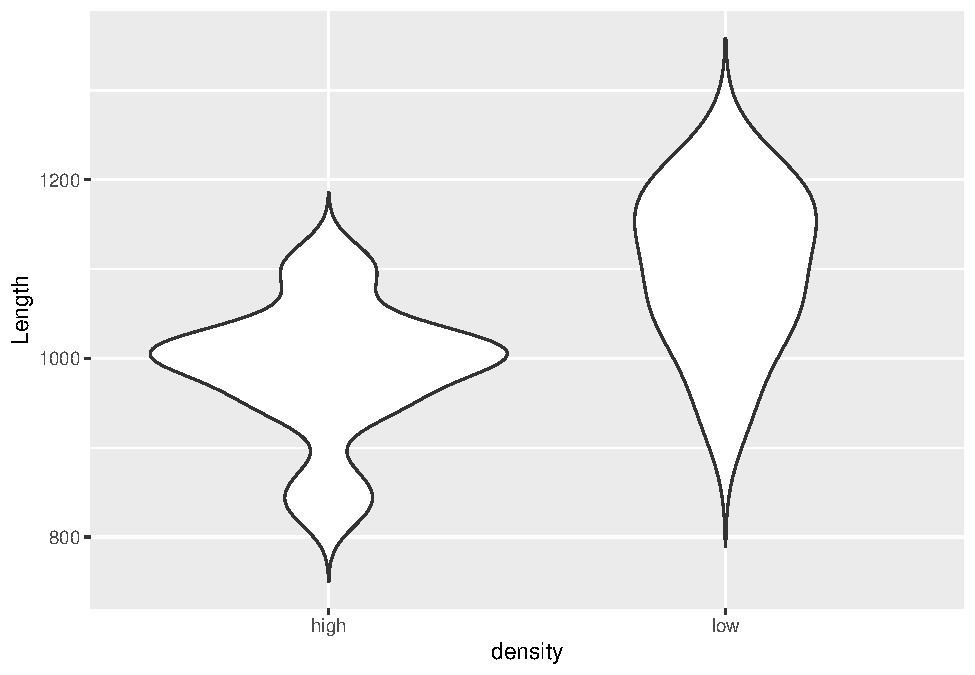
\includegraphics{worstr_files/figure-latex/unnamed-chunk-175-1.pdf}

Here is a much better plot. Not that much more difficult to make, and doesn't make you want to puke even if the code does a little bit.

\begin{Shaded}
\begin{Highlighting}[]
\NormalTok{mid_carps }\OperatorTok
\KeywordTok{ggplot}\NormalTok{(}\KeywordTok{aes}\NormalTok{(}\DataTypeTok{x =}\NormalTok{ density, }\DataTypeTok{y =}\NormalTok{ Length, }\DataTypeTok{fill =}\NormalTok{ density, }\DataTypeTok{color =}\NormalTok{ density)) }\OperatorTok{+}\StringTok{ }
\StringTok{  }\KeywordTok{geom_violin}\NormalTok{(}\KeywordTok{aes}\NormalTok{(}\DataTypeTok{group =}\NormalTok{ density), }\DataTypeTok{trim =} \OtherTok{FALSE}\NormalTok{, }\DataTypeTok{size =} \FloatTok{.75}\NormalTok{) }\OperatorTok{+}
\StringTok{  }\KeywordTok{scale_x_discrete}\NormalTok{(}\DataTypeTok{breaks=}\KeywordTok{c}\NormalTok{(}\StringTok{"high"}\NormalTok{, }\StringTok{"low"}\NormalTok{), }\DataTypeTok{labels =} \KeywordTok{c}\NormalTok{(}\StringTok{"High"}\NormalTok{, }\StringTok{"Low"}\NormalTok{)) }\OperatorTok{+}
\StringTok{  }\KeywordTok{scale_fill_grey}\NormalTok{(}\DataTypeTok{start =} \FloatTok{0.9}\NormalTok{, }\DataTypeTok{end =} \FloatTok{0.4}\NormalTok{) }\OperatorTok{+}
\StringTok{  }\KeywordTok{scale_color_grey}\NormalTok{(}\DataTypeTok{start =} \FloatTok{0.8}\NormalTok{, }\DataTypeTok{end =} \FloatTok{0.3}\NormalTok{) }\OperatorTok{+}
\StringTok{  }\KeywordTok{xlab}\NormalTok{(}\StringTok{"Density"}\NormalTok{) }\OperatorTok{+}
\StringTok{  }\KeywordTok{ylab}\NormalTok{(}\StringTok{"Total length (mm) at age 10"}\NormalTok{) }\OperatorTok{+}
\StringTok{  }\KeywordTok{labs}\NormalTok{(}\DataTypeTok{fill =} \StringTok{"Density"}\NormalTok{, }\DataTypeTok{color =} \StringTok{"Density"}\NormalTok{) }\OperatorTok{+}
\StringTok{  }\KeywordTok{theme_bw}\NormalTok{() }\OperatorTok{+}
\StringTok{  }\KeywordTok{theme}\NormalTok{(}
    \DataTypeTok{axis.title.x =} \KeywordTok{element_text}\NormalTok{(}\DataTypeTok{vjust =} \DecValTok{-1}\NormalTok{),}
    \DataTypeTok{axis.title.y =} \KeywordTok{element_text}\NormalTok{(}\DataTypeTok{vjust =} \DecValTok{3}\NormalTok{),}
    \DataTypeTok{panel.grid =} \KeywordTok{element_blank}\NormalTok{()}
\NormalTok{  )}
\end{Highlighting}
\end{Shaded}

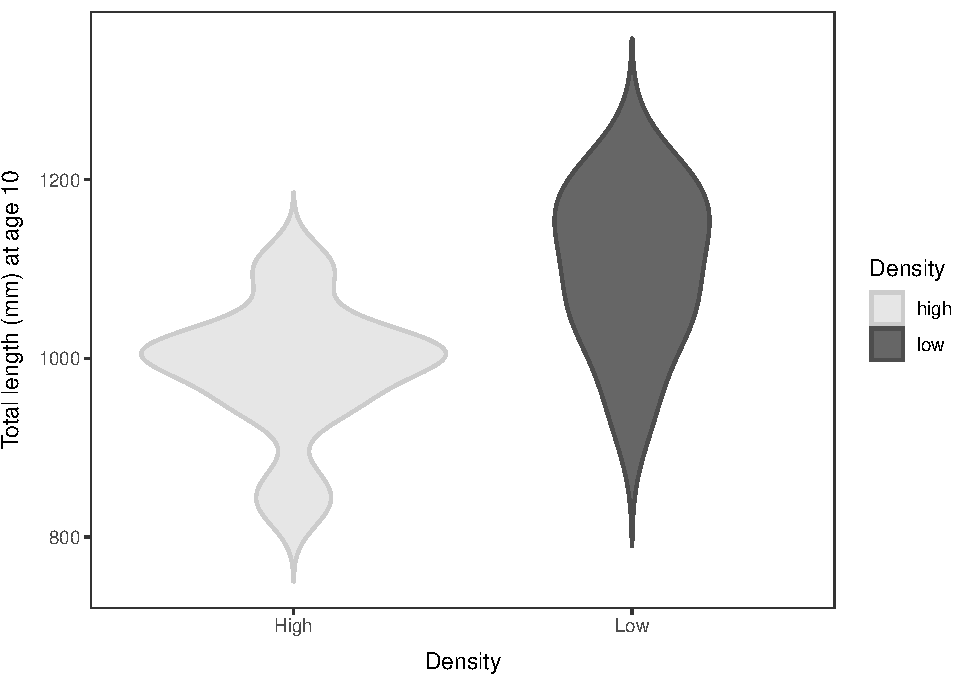
\includegraphics{worstr_files/figure-latex/unnamed-chunk-176-1.pdf}

There, isn't that fancy? I think that gives you a much more detailed understanding of how \texttt{Length} varies between \texttt{high} and \texttt{low} population density than a simple p-value. But, maybe its just me\ldots{}

\hypertarget{frequency-analysis}{%
\section{Frequency analysis}\label{frequency-analysis}}

Now, what if we didn't collect very good data, or we binned our data into low-resolution categories for the sake of ease in our study design? Often, and for a variety of reasons other than crappy data collection, we want to compare frequencies of events between two (or more) groups. We may even design studies specifically to test these kinds of hypotheses when we think about rates, for example. This is very common in studies of population genetics {[}definitely citations available for that one - go Google them{]}

The simplest way to test for differences in the frequency of a categorical response between two groups is (some would argue) the \(\chi^2\) test. The \(\chi^2\) is another one of those that you should really work out by hand because it is used in a variety of settings ``under the hood'' of more complex routines. Here is your token \href{https://www.youtube.com/watch?v=V4SRgabFbz0}{video link showing an example}. Watch it. Please.

\hypertarget{worked-example}{%
\subsection{Worked example}\label{worked-example}}

Let's say we want to know if the number of grass carp in a given age group (say age 10) varies between years. These fish are sterile hybrids, so we would expect that the number of fish in each age would change drastically with increasing time since the year of initial stocking (1995).

First, make a table showing the number of fish in each \texttt{Age} by \texttt{Year} with the \texttt{grasscarp} data.

\begin{Shaded}
\begin{Highlighting}[]
\NormalTok{agexyear <-}\StringTok{ }\KeywordTok{with}\NormalTok{(grasscarp, }\KeywordTok{table}\NormalTok{(Age, Year))}

\KeywordTok{print}\NormalTok{(agexyear)}
\end{Highlighting}
\end{Shaded}

\begin{verbatim}
##     Year
## Age  2006 2007 2009 2010 2017
##   1     0    0    0    2    0
##   2     6    7    7    8    0
##   3    11   10   10   14    3
##   4     4    3    6    3    3
##   5     0    1    3    2   10
##   6     0    1    2    1   12
##   7     0    0    1    3   11
##   8     0    1    1    2   12
##   9     1    0    1    3   21
##   10    4    1    1    2   21
##   11    4    9    0    6   15
##   12    3   15    2    3   18
##   13    0    1    4    3    7
##   14    0    0   11    8    6
##   15    0    0    2   12   12
##   16    0    0    0    2   10
##   17    0    0    0    0    8
##   18    0    0    0    0    9
##   19    0    0    0    0   12
##   20    0    0    0    0   12
##   21    0    0    0    0    5
##   22    0    0    0    0    3
##   23    0    0    0    0    2
\end{verbatim}

Basically what we are going to do is analyze the proportion of total fish in each column by age.

You should see some pretty obvious patterns here. We have a couple of things to think about now. First, this is the kind of question you don't need statistics for. Second, we have a whole bunch of empty groups, and these are not random with respect to year. Some of these come from ages that were not yet available in years 2006 - 2010 and some from patterns in fish stocking. The large number of empty pairings and the fact that most age classes had fewer than five fish in any year prior to 2017 means we should probably break the data down a little further. This stinks because we lose resolution, but that is the cost.

For the sake of demonstration, let's summarize the data by \texttt{high} and \texttt{low} density again and we'll look at the number of fish collected in each age class during high and low density years.

\begin{Shaded}
\begin{Highlighting}[]
\NormalTok{freqs <-}\StringTok{ }\NormalTok{grasscarp }\OperatorTok\StringTok{ }\CommentTok{# Pass grass carp data frame to group_by()}
\StringTok{    }\KeywordTok{filter}\NormalTok{(Age }\OperatorTok\StringTok{ }\KeywordTok{c}\NormalTok{(}\DecValTok{10}\OperatorTok{:}\DecValTok{15}\NormalTok{)) }\CommentTok{# Select only shared age range}

\KeywordTok{head}\NormalTok{(freqs)}
\end{Highlighting}
\end{Shaded}

\begin{verbatim}
##   Year Length Weight_kg Age cohort n_stocked     n acre   ha nha     kg kg_ha
## 1 2006   1262    23.154  12   1994      7000 25128 2957 1203  21 129929   108
## 2 2006   1138    23.923  10   1996      7000 25128 2957 1203  21 129929   108
## 3 2006   1187    18.614  10   1996      7000 25128 2957 1203  21 129929   108
## 4 2006   1207    19.522  12   1994      7000 25128 2957 1203  21 129929   108
## 5 2006   1086    21.285  10   1996      7000 25128 2957 1203  21 129929   108
## 6 2006   1095    18.160  12   1994      7000 25128 2957 1203  21 129929   108
##   density
## 1     low
## 2     low
## 3     low
## 4     low
## 5     low
## 6     low
\end{verbatim}

We will test the null hypothesis that there is no difference in the number of age-10 fish between high and low densities.

\begin{Shaded}
\begin{Highlighting}[]
\CommentTok{# Run the test}
\NormalTok{chi_test <-}\StringTok{ }\KeywordTok{with}\NormalTok{(freqs, }\KeywordTok{chisq.test}\NormalTok{(}\DataTypeTok{x =}\NormalTok{ density, }\DataTypeTok{y =}\NormalTok{ Age))}

\CommentTok{# Have a look}
\KeywordTok{print}\NormalTok{(chi_test)}
\end{Highlighting}
\end{Shaded}

\begin{verbatim}
## 
## 	Pearson's Chi-squared test
## 
## data:  density and Age
## X-squared = 13.107, df = 5, p-value = 0.0224
\end{verbatim}

And, bam! We see that there is a difference in the frequency of fish collected in each age class in high and low density years. Shocker.

Data visualization techniques for contingency table analyses like this seem to have generally lagged behind theory in terms of wide-spread implementation. There is a base R \texttt{mosaicplot} that plots relative freqencies. You can interpret the width of the bars as the proportion of total observations in each age class. Likewise, the height of the vertical segnmens corresponds to proportion of \texttt{high} or \texttt{low} \texttt{density} observations in each \texttt{Age}.

\begin{Shaded}
\begin{Highlighting}[]
\KeywordTok{mosaicplot}\NormalTok{(Age }\OperatorTok{~}\StringTok{ }\NormalTok{density, }\DataTypeTok{data =}\NormalTok{ freqs)}
\end{Highlighting}
\end{Shaded}

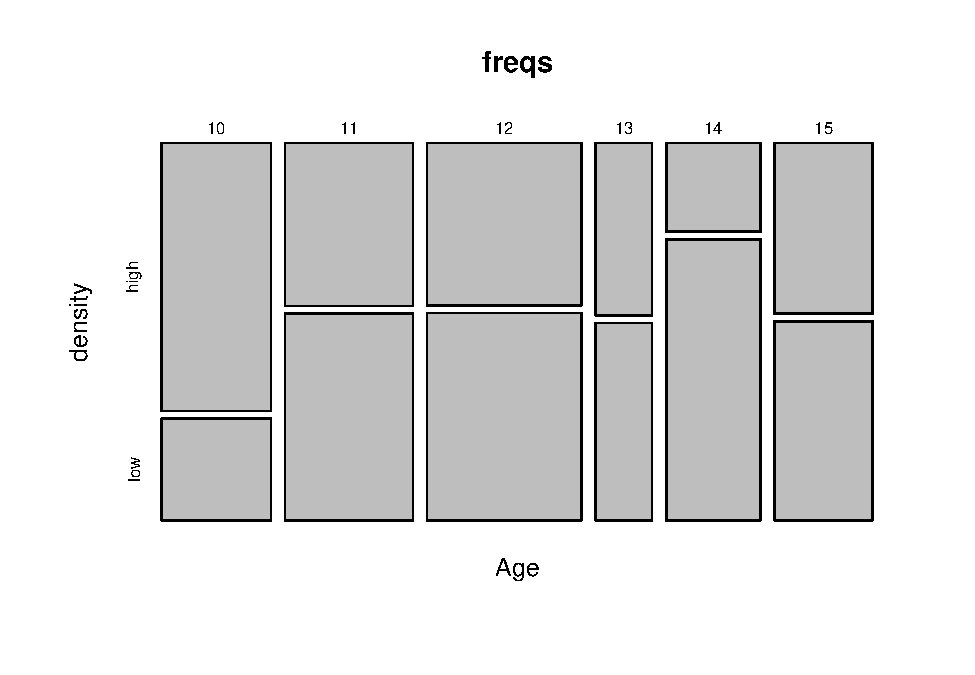
\includegraphics{worstr_files/figure-latex/unnamed-chunk-180-1.pdf}

The need for improved graphical representation for these data types is recognized. There have been recent efforts to extend the philosophies used \texttt{ggplot()} to contingency analysis by r developers (see Wickham and Hofmann 2011). It was even the topic of a recent master's thesis (see Grant 2017). But as far as I know the ideas from these works have not been integrated into \texttt{ggplot2} or the \texttt{tidyverse} yet. Sorry about the citations. I don't know what I was thinking. This is supposed to be the Worst Stats Text eveR.

\hypertarget{next6}{%
\section{Next steps}\label{next6}}

In this chapter, we introduced inferential statistics and walked through examples of a few simple statistical tests for comparing samples to one another using two-sample tests, or to a single value using a one-sample test. In \protect\hyperlink{Chapter7}{Chapter 7} we will continue to build on these tools as we press on to linear models and the rest of statistics.

\hypertarget{Chapter7}{%
\chapter{Linear models}\label{Chapter7}}

Yeah, I know this is the picture from Chapter 4. I only have like five pictures. This is the Worst Stats Text eveR! But, both of the graphs in this picture are just applications of linear regression, which is one kind of linear model, which is also called the general linear model.

Introduction

In this chapter, we will introduce a class of statistical tools known collectively as \textbf{linear models}. This class of tools includes such examples as analysis of variance (ANOVA), linear regression and correlation, and by extension includes n-way ANOVA, multiple linear regression, and analysis of covariance (ANCOVA). Later this semester, we will see that these models be extended even further to include generalized linear models, generalized linear mixed models, multivariate techniques and even machine learning algorithms.

Linear models are, therefore, the gateway into the rest of the world of statistics. We will focus primarily on parametric applications this week and next. The over-arching theme for this week is that any of these methods can be expressed as the formula for a line, which is how they got their names (oh, snap!). We will start with ANOVA because it is analogous to many of the methods that we've already discussed. However, it is important to recognize that this is just a special case of the linear model. This will help you think about how we test statistical assumptions, test hypotheses, and communicate results of models.

Because we are now entering into the realm of `the rest of statistics' we also need to start `talking the talk' in addition to `walking the walk', so we will practice how to write methods sections for these tests and how to report the results. In reality, once you are comfortable using a couple of functions in R, writing up the methods and results is more challenging than fitting models.

\begin{Shaded}
\begin{Highlighting}[]
\KeywordTok{library}\NormalTok{(tidyverse)}
\end{Highlighting}
\end{Shaded}

\hypertarget{anova}{%
\section{Analysis of variance (ANOVA)}\label{anova}}

We will use some of the built-in datasets in R this week to demonstrate our analyses and show how to communicate the methods and the results of our statistical inference.

Analysis of variance is typically used when we have a continuous dependent variable (y, response) and a categorical independent variable (x, explanatory) containing three or more groups. As with the t-test, we assume that the error (variance) within groups is normal (we'll discuss in detail in \protect\hyperlink{Chapter8}{Chapter 8}). Most of the math behind ANOVA is basically the same as a t-test, but we add a couple steps for the third group, and now it essentially becomes the same thing as an F test (\texttt{var.test()} from Chapter 6{[}\#Chapter6{]}) on three groups. In fact, the t-test, the F test, and one-way anova are all pretty much the same thing!

\texttt{mind\ ==\ blown}

\hypertarget{one-way}{%
\subsection{One-way analysis of variance}\label{one-way}}

The number of grouping variables used in ANOVA confers different fancy naming conventions. The simplest of these contains a single grouping variable (e.g.~treatment \textbf{or} year) and is referred to as one-way ANOVA. In theory, these models can be extended to include any number \emph{n} of grouping variables (e.g.~treatment \textbf{and} year) and are commonly referred to as \emph{n}-way ANOVA.

Let's start by loading the \texttt{PlantGrowth} dataset in R:

\begin{Shaded}
\begin{Highlighting}[]
\KeywordTok{data}\NormalTok{(PlantGrowth)}
\end{Highlighting}
\end{Shaded}

\texttt{PlantGrowth} is a dataframe with 30 observations of two variables. The first variable \texttt{weight} describes plant growth (in units of mass), and the second variable \texttt{group} contains control (\texttt{ctrl}) and two treatment groups (\texttt{trt1} and \texttt{trt2}) for individual plants. Have a look, as always:

\begin{Shaded}
\begin{Highlighting}[]
\KeywordTok{str}\NormalTok{(PlantGrowth)}
\end{Highlighting}
\end{Shaded}

\begin{verbatim}
## 'data.frame':	30 obs. of  2 variables:
##  $ weight: num  4.17 5.58 5.18 6.11 4.5 4.61 5.17 4.53 5.33 5.14 ...
##  $ group : Factor w/ 3 levels "ctrl","trt1",..: 1 1 1 1 1 1 1 1 1 1 ...
\end{verbatim}

Let's begin by using a one-way ANOVA to determine if the mass of plants differs between groups in \texttt{PlantGrowth}. In practice, this is \emph{very} easy. First of all, though, we would report our \textbf{methods} something like this:

\begin{quote}
We used a one-way analysis of variance (ANOVA) to estimate the effects of treatment group on the mass (g) of plants assuming a Type-I error rate of \(\alpha\) = 0.05. Our null hypothesis was that all group means were equal (H\textsubscript{0}: \(\mu_{ctrl} = \mu_{trt1} = \mu_{trt2}\)).
\end{quote}

Therefore, if any one of the means is not equal to the others, then we reject the null hypothesis.

You can fit an ANOVA using either the \texttt{aov()} function or the \texttt{lm()} function in base R. I prefer to use \texttt{lm()} for two reasons. First, there is output from \texttt{lm()} that I don't get with \texttt{aov()}. Second, the \texttt{lm()} function is the one we'll use for linear regression, multiple regression, and analysis of covariance. This reminds us that these models are all special cases of the glorious, over-arching group of general linear models \protect\hyperlink{Chapter8}{Chapter 8} and will help us develop a standard workflow moving forward.

\begin{Shaded}
\begin{Highlighting}[]
\CommentTok{# Fit the model}
\NormalTok{model <-}\StringTok{ }\KeywordTok{lm}\NormalTok{(weight}\OperatorTok{~}\NormalTok{group, }\DataTypeTok{data=}\NormalTok{PlantGrowth)}

\CommentTok{# Print the model object to the console}
\NormalTok{model}
\end{Highlighting}
\end{Shaded}

\begin{verbatim}
## 
## Call:
## lm(formula = weight ~ group, data = PlantGrowth)
## 
## Coefficients:
## (Intercept)    grouptrt1    grouptrt2  
##       5.032       -0.371        0.494
\end{verbatim}

Wow, that is dangerously easy to do. But, this output is not very useful for getting the information we need if you don't already know what you are looking at. What we get here is essentially just one part of the information that we would like to (should) report.

We'll proceed with a more standard ANOVA table for now using the \texttt{anova()} function:

\begin{Shaded}
\begin{Highlighting}[]
\CommentTok{# Save anova table to an object}
\NormalTok{plant_nova <-}\StringTok{ }\KeywordTok{anova}\NormalTok{(model)}

\CommentTok{# Have a look at the goodness}
\KeywordTok{print}\NormalTok{(plant_nova)}
\end{Highlighting}
\end{Shaded}

\begin{verbatim}
## Analysis of Variance Table
## 
## Response: weight
##           Df  Sum Sq Mean Sq F value  Pr(>F)  
## group      2  3.7663  1.8832  4.8461 0.01591 *
## Residuals 27 10.4921  0.3886                  
## ---
## Signif. codes:  0 '***' 0.001 '**' 0.01 '*' 0.05 '.' 0.1 ' ' 1
\end{verbatim}

Okay, this is really what we needed in order to evaluate our null hypothesis: an ANOVA table with a break down of the residuals, mean squared errors, and test statistic(s). We interpret the test statistic and the p-value the same way we did in \protect\hyperlink{Chapter6}{Chapter 6} when we did t-tests and Wilcox tests. And, we can now say:

\begin{quote}
We found that the treatment had a significant effect on plant weight
(ANOVA, F = 4.846, df\textsubscript{1} = 2, df\textsubscript{2} = 27, p = 0.0159).
\end{quote}

We can also calculate the R\textsuperscript{2} value for the ANOVA, which is a statistic used to describe the amount of variation in the data explained by the model relative to the total variation in the data set. More correctly, we are actually comparing the sum of squared errors for the model we fit (SSB) to the total sum of squares (SST = SSB + SSE).

For what it's worth, this is a super useful statistic for getting the big-picture perspective on whether your model is useful or crap. You calculate it pretty easily from the \texttt{anova()} output like as:

\[R^2 = \frac{SSB}{SST}\]
\ldots or\ldots{}

Why wouldn't you do this in R?

\begin{Shaded}
\begin{Highlighting}[]
\CommentTok{# Look at the names of the anova() output}
\CommentTok{# We want the "Sum Sq" bit}
\KeywordTok{names}\NormalTok{(plant_nova)}
\end{Highlighting}
\end{Shaded}

\begin{Shaded}
\begin{Highlighting}[]
\CommentTok{# Here is the sum of squares for the model}
\CommentTok{# Have to use back-ticks for spaces, sigh}
\NormalTok{ssb <-}\StringTok{ }\NormalTok{plant_nova}\OperatorTok{$}\StringTok{`}\DataTypeTok{Sum Sq}\StringTok{`}\NormalTok{[}\DecValTok{1}\NormalTok{]}

\CommentTok{# And the sum of squares total is the sum}
\CommentTok{# of the column in this case}
\NormalTok{sst <-}\StringTok{ }\KeywordTok{sum}\NormalTok{(plant_nova}\OperatorTok{$}\StringTok{`}\DataTypeTok{Sum Sq}\StringTok{`}\NormalTok{)}

\CommentTok{# Some quick division, and we get...}
\NormalTok{R2 <-}\StringTok{ }\NormalTok{ssb}\OperatorTok{/}\NormalTok{sst}
\end{Highlighting}
\end{Shaded}

Have a look:

\begin{Shaded}
\begin{Highlighting}[]
\KeywordTok{print}\NormalTok{(R2)}
\end{Highlighting}
\end{Shaded}

\begin{verbatim}
## [1] 0.2641483
\end{verbatim}

Now, we can say that our treatment effect explained about 26\% of the variation in the data. The rest is a combination error and unexplained variation in the data that might require further investigation.

The only problem here is that this is an awful lot of work to get something that should be really easy to do in R. And, we still don't know how \texttt{weight} varied between \texttt{groups}. We just know that at least one group is different from the other.

Thankfully, the default output of \texttt{summary()} for linear models fit with \texttt{lm()} does a lot of this for us.

\begin{Shaded}
\begin{Highlighting}[]
\CommentTok{# Print the summary of the model}
\KeywordTok{summary}\NormalTok{(model)}
\end{Highlighting}
\end{Shaded}

\begin{verbatim}
## 
## Call:
## lm(formula = weight ~ group, data = PlantGrowth)
## 
## Residuals:
##     Min      1Q  Median      3Q     Max 
## -1.0710 -0.4180 -0.0060  0.2627  1.3690 
## 
## Coefficients:
##             Estimate Std. Error t value Pr(>|t|)    
## (Intercept)   5.0320     0.1971  25.527   <2e-16 ***
## grouptrt1    -0.3710     0.2788  -1.331   0.1944    
## grouptrt2     0.4940     0.2788   1.772   0.0877 .  
## ---
## Signif. codes:  0 '***' 0.001 '**' 0.01 '*' 0.05 '.' 0.1 ' ' 1
## 
## Residual standard error: 0.6234 on 27 degrees of freedom
## Multiple R-squared:  0.2641,	Adjusted R-squared:  0.2096 
## F-statistic: 4.846 on 2 and 27 DF,  p-value: 0.01591
\end{verbatim}

That's better, we get some useful information here. First of all, we get the value of the test statistic, the df, and the p-value for the model. We also get the \(R^2\) for the model, 0.26, as part of the default output.

But, what if we want to know more about how treatment affected weight? Like, which groups are different? Can we use the p-values reported in the column \texttt{Pr(\textgreater{}\textbar{}t\textbar{})} to infer group-wise differences? The quick answer is ``sometimes''.

The \texttt{Coefficients} chunk of this output can help us with inference in simple situations, and it really is the key to making predictions from our models (see \protect\hyperlink{Chapter10}{Chapter 10}).

Remember, most model output in R is stored as lists, so we can extract the coefficients table like this if we look at `names( summary(model) ) to find what we want:

\begin{Shaded}
\begin{Highlighting}[]
\NormalTok{coeffs <-}\StringTok{ }\KeywordTok{data.frame}\NormalTok{( }\KeywordTok{summary}\NormalTok{(model)}\OperatorTok{$}\NormalTok{coefficients )}
\end{Highlighting}
\end{Shaded}

Okay, what is going on here? This looks nothing like the output we got from \texttt{anova()}.

The \texttt{coeffs} object is a dataframe with columns for mean coefficient estimates, the standard error of those estimates, t-statistic, and p-value. We are actually not going to worry about the p-values here for a hot minute.

Let's focus on the estimate column first. There are three values here. Each of these represents one of the factor levels in the \texttt{group} variable in \texttt{PlantGrowth}. They are assigned alpha-numerically, and the first (\texttt{ctrl}) is assigned as the \texttt{(Intercept)} or base level against which all others are compared. In this sense, the \texttt{(Intercept)} coefficient is an estimate of the mean value of \texttt{weight} for the \texttt{group} called \texttt{ctrl.}

Do a quick check:

\begin{Shaded}
\begin{Highlighting}[]
\CommentTok{# Calculate and print mean weight}
\CommentTok{# for the group ctrl in PlantGrowth}
\NormalTok{PlantGrowth }\OperatorTok
\StringTok{  }\KeywordTok{filter}\NormalTok{(group }\OperatorTok{==}\StringTok{ 'ctrl'}\NormalTok{) }\OperatorTok
\StringTok{  }\KeywordTok{summarize}\NormalTok{(}\DataTypeTok{avg =} \KeywordTok{mean}\NormalTok{(weight))}
\end{Highlighting}
\end{Shaded}

\begin{verbatim}
##     avg
## 1 5.032
\end{verbatim}

As you can see, the prediction from the ANOVA is identical to the group mean estimated directly from the data.

The coefficients for \texttt{grouptrt1} and \texttt{grouptrt2} can be thought of adjustments to the \texttt{(Intercept)} coefficient, or the difference between the mean of \texttt{ctrl} and \texttt{trt1} or \texttt{trt2}. If the \texttt{Estimate} for \texttt{grouptrt1} or \texttt{grouptrt2} is negative, then the mean for that group is less than \texttt{ctrl} and if it is positive, the mean for the group is greater than \texttt{ctrl}.

If we wanted to calculate the mean \texttt{weight} of the \texttt{trt1} and \texttt{trt2} groups, we would add them to the \texttt{(Intercept)} coefficient like this:

\begin{Shaded}
\begin{Highlighting}[]
\CommentTok{# Assign model coefficients to objects}
\NormalTok{ctrl <-}\StringTok{ }\NormalTok{coeffs}\OperatorTok{$}\NormalTok{Estimate[}\DecValTok{1}\NormalTok{]}
\NormalTok{trt1 <-}\StringTok{ }\NormalTok{coeffs}\OperatorTok{$}\NormalTok{Estimate[}\DecValTok{2}\NormalTok{]}
\NormalTok{trt2 <-}\StringTok{ }\NormalTok{coeffs}\OperatorTok{$}\NormalTok{Estimate[}\DecValTok{3}\NormalTok{]}

\CommentTok{# Calculate group means for trt1 and trt2}
\CommentTok{# from the model}
\NormalTok{trt1_prediction <-}\StringTok{ }\NormalTok{ctrl }\OperatorTok{+}\StringTok{ }\NormalTok{trt1}
\NormalTok{trt2_prediction <-}\StringTok{ }\NormalTok{ctrl }\OperatorTok{+}\StringTok{ }\NormalTok{trt2}

\KeywordTok{print}\NormalTok{(}\KeywordTok{c}\NormalTok{(trt1_prediction, trt2_prediction))}
\end{Highlighting}
\end{Shaded}

\begin{verbatim}
## [1] 4.661 5.526
\end{verbatim}

If you calculate the means for these groups directly from the data you'll see that these values are identical to the mean \texttt{weight} of the \texttt{trt1} and \texttt{trt2} groups.

In \protect\hyperlink{Chapter10}{Chapter 10} we will examine how to estimate confidence intervals around these estimates and make predictions from the model that include our uncertainty. But for that, we'll need to talk about a little bit of math and we're dealing with enough right now already!

Finally, the p-values associated with \texttt{trt1} and \texttt{trt2} indicates whether each group is significantly different from \texttt{ctrl}. In the case of the intercept, the p-value simply tells us whether the mean \texttt{weight} of \texttt{ctrl} is significantly different from zero. A fundamentally dull question - of course it is. This is the first time we really need to think about the differences between our statistical null hypotheses and our biological null hypotheses.

If we want to do further comparisons between groups (other than just comparing \texttt{trt1} and \texttt{trt2} to \texttt{ctrl} by themselves), then we need to add on a little ``post-hoc'' testing to find out which groups differ. We can use a `pair-wise' comparison to test for differences between factor levels. Because this essentially means conducting a whole bunch of t-tests, we need a way to account for our repeated Type-I error rate, because at \(\alpha\) = 0.05 we stand a 1 in 20 chance of falsely rejecting the null even if it is true.

One tool that allows us to make multiple comparisons between groups while adjusting for elevated Type-I error is the Tukey HSD (honest significant difference) test. This test makes comparisons between each pairing of groups while controlling for Type-I error. Essentially, this makes it harder to detect differences between groups but when we do we are more sure that they are not spurious (``Honest significant difference'', say it with me).

Sound confusing? At least it's easy to do in R.

We need to recast our model this as an \texttt{aov} object in R\ldots this is essentially the same thing as the \texttt{lm} function, but in a different wrapper (literally) that allows us to access the info in a different way. It would be a fine default function for doing ANOVA if we weren't interested in going any further with linear models.

\begin{Shaded}
\begin{Highlighting}[]
\KeywordTok{TukeyHSD}\NormalTok{(    }\CommentTok{# The function that does the Tukey test}
  \KeywordTok{aov}\NormalTok{(       }\CommentTok{# A wrapper for lm objects}
\NormalTok{    model    }\CommentTok{# The model that we ran above}
\NormalTok{    )}
\NormalTok{  )}
\end{Highlighting}
\end{Shaded}

\begin{verbatim}
##   Tukey multiple comparisons of means
##     95% family-wise confidence level
## 
## Fit: aov(formula = model)
## 
## $group
##             diff        lwr       upr     p adj
## trt1-ctrl -0.371 -1.0622161 0.3202161 0.3908711
## trt2-ctrl  0.494 -0.1972161 1.1852161 0.1979960
## trt2-trt1  0.865  0.1737839 1.5562161 0.0120064
\end{verbatim}

This report shows us exactly how \texttt{weight} differs between each pair of treatment groups. Here, we see that the only significant difference (\texttt{p\ adj\ \textless{}\ 0.05}) occurs between \texttt{trt2} and \texttt{trt1}.

For the readers, and for us, it may be easier to see this information displayed graphically:

\begin{Shaded}
\begin{Highlighting}[]
\CommentTok{# Make a boxplot of weight by group}
\CommentTok{# using the PlantGrowth data and }
\CommentTok{# base graphics}
\KeywordTok{boxplot}\NormalTok{(}
\NormalTok{  weight}\OperatorTok{~}\NormalTok{group,           }\CommentTok{# Relationship of interest as formula}
  \DataTypeTok{data=}\NormalTok{PlantGrowth,       }\CommentTok{# Name of the data set}
  \DataTypeTok{col=}\StringTok{'gray'}\NormalTok{,             }\CommentTok{# Fill color for boxes}
  \DataTypeTok{ylab=}\StringTok{'Mass (g)'}\NormalTok{,        }\CommentTok{# Y-axis label}
  \DataTypeTok{xlab=}\StringTok{'Treatment group'}\NormalTok{, }\CommentTok{# X-axis label}
  \DataTypeTok{boxwex=}\NormalTok{.}\DecValTok{25}
\NormalTok{  )}
\end{Highlighting}
\end{Shaded}

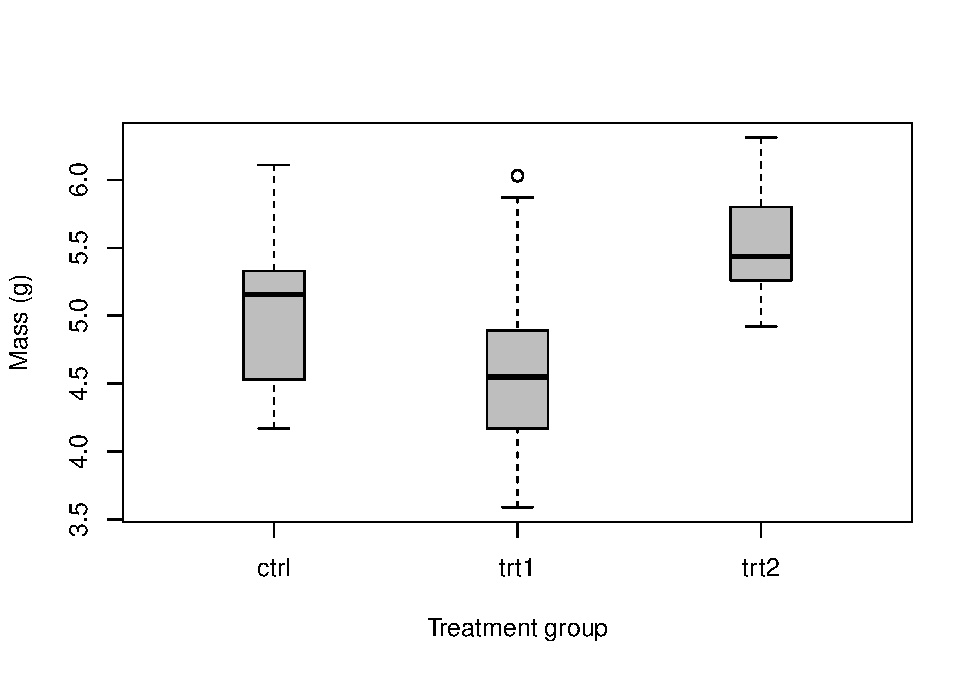
\includegraphics{worstr_files/figure-latex/unnamed-chunk-194-1.pdf}

In addition to what we wrote before, we can now say something along the lines of:

\begin{quote}
``We found that the mass of plants in the trt2 group (5.5 \(\pm\) 0.4 g) was significantly greater than plants in the trt1 group (4.7 \(\pm\) 0.8 g; Tukey HSD, p = 0.012). However, we failed to detect differences in mass between plants in the control group (5.0 \(\pm\) 0.6 g) and trt1 (p = 0.39) or trt2 (p = 0.20).''
\end{quote}

\hypertarget{twon-way-anova}{%
\subsection{\texorpdfstring{Two(\emph{n})-way ANOVA}{Two(n)-way ANOVA}}\label{twon-way-anova}}

Next, we'll step up the complexity and talk about cases for which we have more than one grouping variable and some kind of numeric response. In these cases, we can use a two-way ANOVA (or `\emph{n}-way' depending on number of factors) to examine effects of more than one grouping variable on the response.

Here, we will use a data set describing differences in the mass of belly- button lint collected from males and females of three species of apes.

\begin{Shaded}
\begin{Highlighting}[]
\CommentTok{# Read in the data:}
\NormalTok{lint <-}\StringTok{ }\KeywordTok{read.csv}\NormalTok{(}\StringTok{'data/lint.txt'}\NormalTok{)}
\end{Highlighting}
\end{Shaded}

\hypertarget{main-effects-7}{%
\subsubsection{Main effects model}\label{main-effects-7}}

Now we can fit a model to the data. This will work the same way as for the one-way ANOVA above, but this time we will add more terms on the right hand side of the equation. We will start by looking at the \emph{main effects} model for this data set.

What is a main-effects model? This model assumes that the response of interest, in this case the mass of belly button lint, \texttt{lintmass}, is affected by both \texttt{species} and \texttt{gender}, and that within species the effect of gender is the same. For example, the mass of belly button lint could be greater in one species compared to others, and if there is a difference between sexes we would expect that trend to be the same across species (e.g., boys always have more lint than girls - sorry guys, it's probably true!).

\begin{Shaded}
\begin{Highlighting}[]
\CommentTok{# Fit the model and save it to an object}
\NormalTok{lint.model<-}\StringTok{ }\KeywordTok{lm}\NormalTok{(lintmass}\OperatorTok{~}\NormalTok{species }\OperatorTok{+}\StringTok{ }\NormalTok{gender, }\DataTypeTok{data =}\NormalTok{ lint)}

\CommentTok{# Look at the summary of the model fit}
\KeywordTok{summary}\NormalTok{(lint.model)}
\end{Highlighting}
\end{Shaded}

\begin{verbatim}
## 
## Call:
## lm(formula = lintmass ~ species + gender, data = lint)
## 
## Residuals:
##     Min      1Q  Median      3Q     Max 
## -2.5792 -0.9021  0.0875  0.8448  2.3917 
## 
## Coefficients:
##                  Estimate Std. Error t value Pr(>|t|)    
## (Intercept)       15.5458     0.6133  25.346  < 2e-16 ***
## speciesSpecies 2  -3.4375     0.7512  -4.576 0.000183 ***
## speciesSpecies 3  -1.8750     0.7512  -2.496 0.021414 *  
## genderMale         4.9083     0.6133   8.003 1.16e-07 ***
## ---
## Signif. codes:  0 '***' 0.001 '**' 0.01 '*' 0.05 '.' 0.1 ' ' 1
## 
## Residual standard error: 1.502 on 20 degrees of freedom
## Multiple R-squared:  0.8096,	Adjusted R-squared:  0.781 
## F-statistic: 28.35 on 3 and 20 DF,  p-value: 2.107e-07
\end{verbatim}

\begin{Shaded}
\begin{Highlighting}[]
\CommentTok{# Print the anova table}
\KeywordTok{anova}\NormalTok{(lint.model)}
\end{Highlighting}
\end{Shaded}

\begin{verbatim}
## Analysis of Variance Table
## 
## Response: lintmass
##           Df  Sum Sq Mean Sq F value    Pr(>F)    
## species    2  47.396  23.698  10.499 0.0007633 ***
## gender     1 144.550 144.550  64.041  1.16e-07 ***
## Residuals 20  45.143   2.257                      
## ---
## Signif. codes:  0 '***' 0.001 '**' 0.01 '*' 0.05 '.' 0.1 ' ' 1
\end{verbatim}

As you can see, the output for the model is much the same as for the one-way ANOVA. The only real difference is that we have more than one grouping variable here. We conclude that there is a significant difference in \texttt{lintmass} between \texttt{species} (F = 10.50, df = 2, p \textless{} 0.05) and between \texttt{genders} (F = 64.01, df = 1, p \textless{} 0.05).

As before, we can make a quick boxplot and overlay our raw data to visualize these differences:

\begin{Shaded}
\begin{Highlighting}[]
\NormalTok{lint }\OperatorTok\StringTok{ }
\StringTok{  }\KeywordTok{ggplot}\NormalTok{(}\KeywordTok{aes}\NormalTok{(}\DataTypeTok{x =}\NormalTok{ species, }\DataTypeTok{y =}\NormalTok{ lintmass, }\DataTypeTok{fill=}\NormalTok{gender)) }\OperatorTok{+}
\StringTok{    }\KeywordTok{geom_boxplot}\NormalTok{() }\OperatorTok{+}
\StringTok{    }\KeywordTok{geom_point}\NormalTok{(}\DataTypeTok{position=}\KeywordTok{position_jitterdodge}\NormalTok{(.}\DecValTok{1}\NormalTok{)) }\OperatorTok{+}
\StringTok{    }\KeywordTok{xlab}\NormalTok{(}\StringTok{'Species'}\NormalTok{) }\OperatorTok{+}
\StringTok{    }\KeywordTok{ylab}\NormalTok{(}\StringTok{'Lint mass'}\NormalTok{) }\OperatorTok{+}
\StringTok{    }\KeywordTok{labs}\NormalTok{(}\DataTypeTok{fill =} \StringTok{"Gender"}\NormalTok{) }\OperatorTok{+}
\StringTok{    }\KeywordTok{theme_bw}\NormalTok{() }\OperatorTok{+}
\StringTok{    }\KeywordTok{theme}\NormalTok{(}\DataTypeTok{axis.title.x =} \KeywordTok{element_text}\NormalTok{(}\DataTypeTok{vjust=}\OperatorTok{-}\DecValTok{1}\NormalTok{),}
          \DataTypeTok{axis.title.y =} \KeywordTok{element_text}\NormalTok{(}\DataTypeTok{vjust=}\DecValTok{3}\NormalTok{),}
          \DataTypeTok{panel.grid =} \KeywordTok{element_blank}\NormalTok{()}
\NormalTok{          )}
\end{Highlighting}
\end{Shaded}

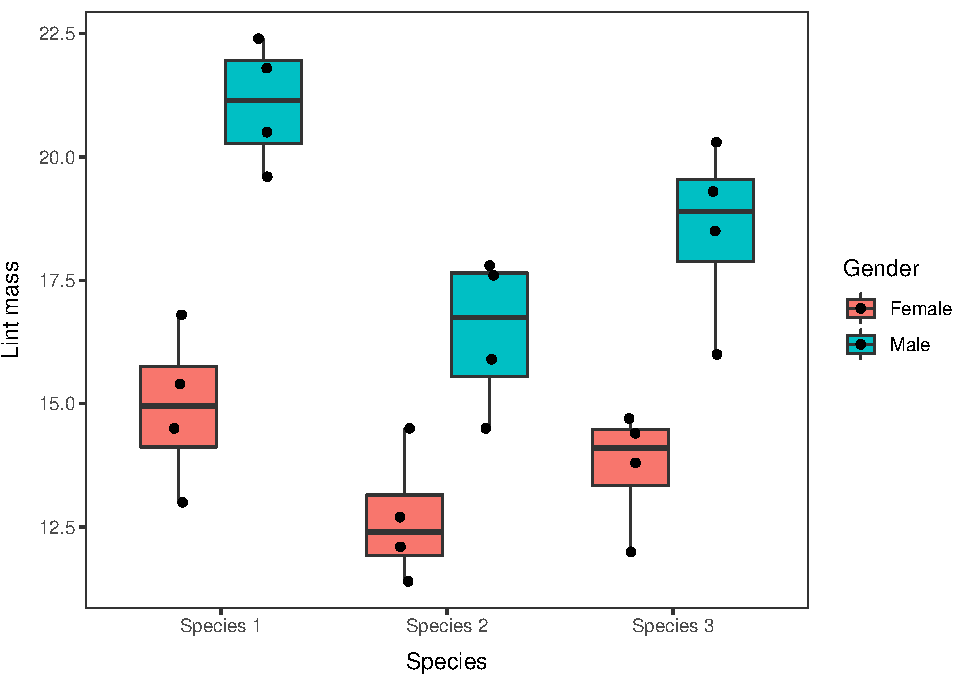
\includegraphics{worstr_files/figure-latex/unnamed-chunk-197-1.pdf}

Hopefully after seeing these results you are now starting to realize how important a few well-placed figures and tables can be for clearly communicating the results of your research (even if it is about belly-button lint).

The math for making predictions becomes a little more complicated once we add a second grouping variable. Even the numbers of pair-wise comparisons can become overwhelming in a simple situation like this. Therefore, we'll hold off on digging too much deeper into the math until next week.

\hypertarget{interaction-terms}{%
\subsubsection{Interaction terms}\label{interaction-terms}}

The n-way ANOVA is the first kind of model we have used in which it is possible to consider \emph{interactions} between two or more factors. An interaction occurs when the effects of two or more factors are not additive. This means that the effect of \texttt{gender} might change for different \texttt{species}. For example, let us consider the following scenario in the \texttt{lint} data.

Perhaps we hypothesize that lint accumulation in the belly buttons of females differs in pattern from males due to social grooming patterns and sex-specific behavioral patterns favoring females in only certain species. As a result, we might expect that \texttt{gender} and \texttt{species} could have some kind of non-additive effect on \texttt{lintmass} in these apes such that there are significant, sex-specific differences only in some species. To test this, we would use the following:

\begin{Shaded}
\begin{Highlighting}[]
\CommentTok{# Fit a new model that includes an interaction, signified by '*'}
\NormalTok{lint.modeli <-}\StringTok{ }\KeywordTok{lm}\NormalTok{(lintmass}\OperatorTok{~}\NormalTok{species }\OperatorTok{*}\StringTok{ }\NormalTok{gender, }\DataTypeTok{data=}\NormalTok{lint)}

\CommentTok{# Summarize the model}
\KeywordTok{summary}\NormalTok{(lint.modeli)}
\end{Highlighting}
\end{Shaded}

\begin{verbatim}
## 
## Call:
## lm(formula = lintmass ~ species * gender, data = lint)
## 
## Residuals:
##    Min     1Q Median     3Q    Max 
## -2.525 -0.750  0.050  1.019  1.875 
## 
## Coefficients:
##                             Estimate Std. Error t value Pr(>|t|)    
## (Intercept)                  14.9250     0.7404  20.159 8.40e-14 ***
## speciesSpecies 2             -2.2500     1.0471  -2.149   0.0455 *  
## speciesSpecies 3             -1.2000     1.0471  -1.146   0.2668    
## genderMale                    6.1500     1.0471   5.874 1.46e-05 ***
## speciesSpecies 2:genderMale  -2.3750     1.4808  -1.604   0.1261    
## speciesSpecies 3:genderMale  -1.3500     1.4808  -0.912   0.3740    
## ---
## Signif. codes:  0 '***' 0.001 '**' 0.01 '*' 0.05 '.' 0.1 ' ' 1
## 
## Residual standard error: 1.481 on 18 degrees of freedom
## Multiple R-squared:  0.8335,	Adjusted R-squared:  0.7873 
## F-statistic: 18.03 on 5 and 18 DF,  p-value: 1.898e-06
\end{verbatim}

\begin{Shaded}
\begin{Highlighting}[]
\CommentTok{# Print an ANOVA table for the model}
\KeywordTok{anova}\NormalTok{(lint.modeli)}
\end{Highlighting}
\end{Shaded}

\begin{verbatim}
## Analysis of Variance Table
## 
## Response: lintmass
##                Df  Sum Sq Mean Sq F value    Pr(>F)    
## species         2  47.396  23.698 10.8079 0.0008253 ***
## gender          1 144.550 144.550 65.9253 1.983e-07 ***
## species:gender  2   5.676   2.838  1.2943 0.2984104    
## Residuals      18  39.468   2.193                      
## ---
## Signif. codes:  0 '***' 0.001 '**' 0.01 '*' 0.05 '.' 0.1 ' ' 1
\end{verbatim}

Alas, in the case of the lint model, this interaction is not significant, so we lack the evidence we would need to say that lint accumulation changes differently between genders within species.

\hypertarget{simple-linear-regression}{%
\section{Simple linear regression}\label{simple-linear-regression}}

We have now considered the case of what to do when we have a numerical response and categorical explanatory variable(s) with any number of groups or grouping variables. But, what if we have both a numerical response and numerical explanatory variables? Fear not, there is a stat for that! Now we are entering the realm of correlation and regression. Next week, we'll show that ANOVA is, in fact, just a special kind of regression.

When we fit a linear regression model, we are trying to explain relationships between some response of interest (dependent variable y) and one or more explanatory (independent) variables, x.

As with all linear models the goal of regression analysis is, in it's simplest sense, to fit a line through all of the points in bivariate space that minimizes the distance between the points and a line of the form:

\[y = mx + b\]

That ought to look familiar!

In the case of statistics, we usually represent the formula for a line like this:

\[Y_i = \beta_0 + \beta_i X_i\]

We are ignoring an important part of these statistical models for now. In most cases, though, we will be estimating a parameter for the intercept and one parameter for each explanatory variable of interest.

\hypertarget{simple-linear-regression-1}{%
\subsection{Simple linear regression}\label{simple-linear-regression-1}}

Since most folks are probably more familiar with linear regression than with ANOVA whether they know it or not, we'll jump right into this one with an example using the \texttt{swiss} data.

These data are for fertility and infant mortality rates as related to a number of socio-economic indicators. Take a moment to look at them:

\begin{Shaded}
\begin{Highlighting}[]
\KeywordTok{data}\NormalTok{(swiss)}
\end{Highlighting}
\end{Shaded}

You can see the description of these data by looking at the help file for the data set as always. Have look on your own:

\begin{Shaded}
\begin{Highlighting}[]
\NormalTok{?swiss}
\end{Highlighting}
\end{Shaded}

Now, let's get cracking.

We'll start by fitting a simple model and then build complexity.

Fit a model that relates fertility to education level. Notice that this looks exactly the same as the call to \texttt{lm} for the ANOVAs above? That's because they are the same thing and people have been lying to you your whole life. Perhaps it took reading The Worst Stats Text eveR to learn it? If so, I aplogize for your misfortune.

\begin{Shaded}
\begin{Highlighting}[]
\CommentTok{# Fit the model and assign it to a named object}
\NormalTok{fert_mod <-}\StringTok{ }\KeywordTok{lm}\NormalTok{(Fertility }\OperatorTok{~}\StringTok{ }\NormalTok{Education, }\DataTypeTok{data =}\NormalTok{ swiss)}

\CommentTok{# Summarize the model}
\KeywordTok{summary}\NormalTok{(fert_mod)}
\end{Highlighting}
\end{Shaded}

\begin{verbatim}
## 
## Call:
## lm(formula = Fertility ~ Education, data = swiss)
## 
## Residuals:
##     Min      1Q  Median      3Q     Max 
## -17.036  -6.711  -1.011   9.526  19.689 
## 
## Coefficients:
##             Estimate Std. Error t value Pr(>|t|)    
## (Intercept)  79.6101     2.1041  37.836  < 2e-16 ***
## Education    -0.8624     0.1448  -5.954 3.66e-07 ***
## ---
## Signif. codes:  0 '***' 0.001 '**' 0.01 '*' 0.05 '.' 0.1 ' ' 1
## 
## Residual standard error: 9.446 on 45 degrees of freedom
## Multiple R-squared:  0.4406,	Adjusted R-squared:  0.4282 
## F-statistic: 35.45 on 1 and 45 DF,  p-value: 3.659e-07
\end{verbatim}

The \texttt{(Intercept)} term in this summary is the y-intercept from our formula for a line and the \texttt{Education} coefficient is the slope of the line. Our intercept tells us that mean \texttt{Fertility} (y) is about 79.6 when \texttt{Education} (x) is zero. Note that this interpretation does not change even if we did not observe an education of zero in the data - something to think about in the weeks to come. The p-value for the intercept just tells us that this value is significantly different from zero (snores).

The p-value for the \texttt{Education} coefficient tells us that the slope of the line is also significantly different from zero. Because this number is negative, we know that there is an inverse relationship between \texttt{Education} and \texttt{Fertility}. In other words, more highly educated individuals have fewer children. You can tell this is an inverse relationship because of the minus sign in front of the coefficient for \texttt{Education}. We know that the relationship is significant because of the small p-value and corresponding significance codes.

We explained a little more than 40\% of the variability in the response with this one explanatory variable if we look at the R\textsuperscript{2} value that is returned (we'll work with the \texttt{Multiple\ R-squared} by default).

This is as far as the summary goes for linear regression for now. That is, we don't need the ANOVA table to assess significance any more because we have no factors - just continuous variables. What we end up with in this summary are the coefficients that can be used to describe the line that passes through the data and minimizes the residual errors (that's the part we ignored above).

\begin{quote}
WHAT??
\end{quote}

Let's explain this by actually looking at the data and plotting our model over the top of it.

First, we'll use the built-in \texttt{predict()} function to create a trend line and a prediction interval. We'll dig deeper into how to do this in \protect\hyperlink{Chapter10}{Chapter 10}.

\begin{Shaded}
\begin{Highlighting}[]
\CommentTok{# Make predictions from the fitted model object using observed data}
\NormalTok{predicted_fertility =}\StringTok{ }\KeywordTok{predict}\NormalTok{(fert_mod, }\DataTypeTok{interval =} \StringTok{'confidence'}\NormalTok{)}

\CommentTok{# Add these to the swiss data}
\NormalTok{swiss_pred <-}\StringTok{ }\KeywordTok{cbind}\NormalTok{(swiss, predicted_fertility)}
\end{Highlighting}
\end{Shaded}

Now, we can plot the raw data as a scatterplot and add our model estimates over the top. You should notice that the confidence interval is much wider at high values of \texttt{Education} because there are few data points and thus more uncertainty in that part of the data.

\begin{Shaded}
\begin{Highlighting}[]
\CommentTok{# Sets up data and aesthetics}
\KeywordTok{ggplot}\NormalTok{(swiss_pred, }
       \KeywordTok{aes}\NormalTok{(}\DataTypeTok{x =}\NormalTok{ Education, }\DataTypeTok{y =}\NormalTok{ Fertility)) }\OperatorTok{+}
\StringTok{  }\CommentTok{# Adds raw data as points}
\StringTok{  }\KeywordTok{geom_point}\NormalTok{(}\DataTypeTok{colour =} \StringTok{'blue'}\NormalTok{, }\DataTypeTok{fill =} \StringTok{'blue'}\NormalTok{, }\DataTypeTok{alpha =} \FloatTok{0.3}\NormalTok{, }\DataTypeTok{size =} \DecValTok{2}\NormalTok{) }\OperatorTok{+}
\StringTok{  }\CommentTok{# Adds regression line}
\StringTok{  }\KeywordTok{geom_line}\NormalTok{( }\KeywordTok{aes}\NormalTok{(}\DataTypeTok{y =}\NormalTok{ fit), }\DataTypeTok{size =} \DecValTok{1}\NormalTok{) }\OperatorTok{+}
\StringTok{  }\CommentTok{# Adds 95% confidence interval}
\StringTok{  }\KeywordTok{geom_ribbon}\NormalTok{(}\KeywordTok{aes}\NormalTok{(}\DataTypeTok{ymin =}\NormalTok{ lwr, }\DataTypeTok{ymax =}\NormalTok{ upr), }\DataTypeTok{color =} \StringTok{'purple'}\NormalTok{, }\DataTypeTok{alpha =} \FloatTok{.2}\NormalTok{) }\OperatorTok{+}
\StringTok{  }\CommentTok{# Adds sweet style tweaks of your choosing}
\StringTok{  }\KeywordTok{theme}\NormalTok{(}\DataTypeTok{legend.position =} \StringTok{"none"}\NormalTok{)}
\end{Highlighting}
\end{Shaded}

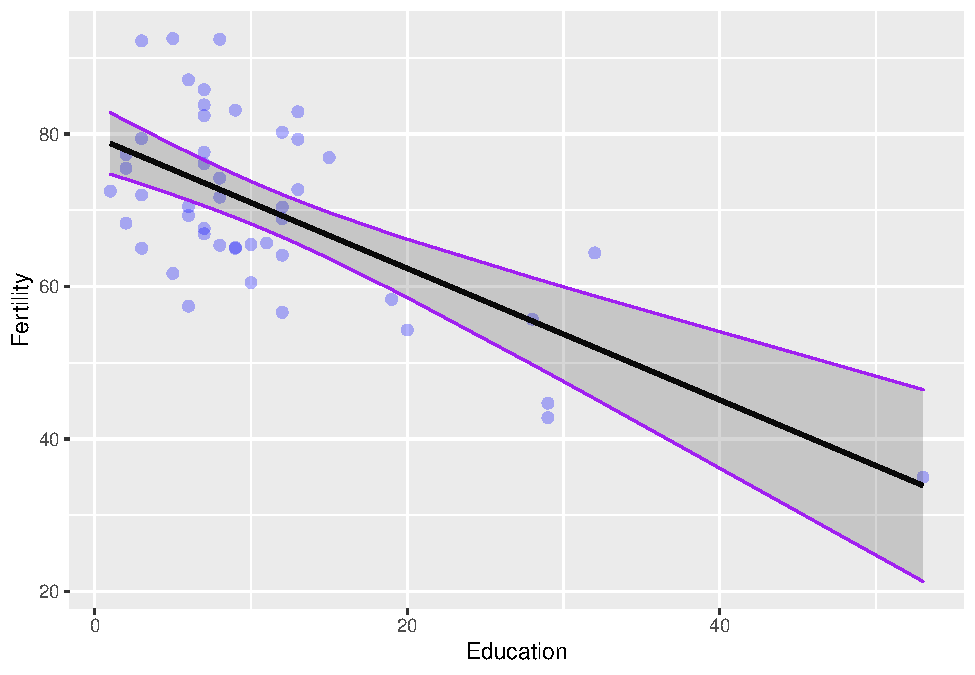
\includegraphics{worstr_files/figure-latex/unnamed-chunk-203-1.pdf}

Again, dangerously easy.

\hypertarget{multiple-linear-regression}{%
\section{Multiple linear regression}\label{multiple-linear-regression}}

We can, of course, extend this to include multiple continuous explanatory variables of interest just as we did with ANOVA for multiple categorical explanatory variables!

Here is an example to whet your appetite. Let's say we want a multiple regression model that includes both \texttt{Education} and \texttt{Catholic}?

\begin{Shaded}
\begin{Highlighting}[]
\NormalTok{multiple_mod <-}\StringTok{ }\KeywordTok{lm}\NormalTok{(Fertility }\OperatorTok{~}\StringTok{ }\NormalTok{Education }\OperatorTok{+}\StringTok{ }\NormalTok{Catholic, }\DataTypeTok{data =}\NormalTok{ swiss)}

\KeywordTok{summary}\NormalTok{(multiple_mod)}
\end{Highlighting}
\end{Shaded}

\begin{verbatim}
## 
## Call:
## lm(formula = Fertility ~ Education + Catholic, data = swiss)
## 
## Residuals:
##     Min      1Q  Median      3Q     Max 
## -15.042  -6.578  -1.431   6.122  14.322 
## 
## Coefficients:
##             Estimate Std. Error t value Pr(>|t|)    
## (Intercept) 74.23369    2.35197  31.562  < 2e-16 ***
## Education   -0.78833    0.12929  -6.097 2.43e-07 ***
## Catholic     0.11092    0.02981   3.721  0.00056 ***
## ---
## Signif. codes:  0 '***' 0.001 '**' 0.01 '*' 0.05 '.' 0.1 ' ' 1
## 
## Residual standard error: 8.331 on 44 degrees of freedom
## Multiple R-squared:  0.5745,	Adjusted R-squared:  0.5552 
## F-statistic:  29.7 on 2 and 44 DF,  p-value: 6.849e-09
\end{verbatim}

Or if we really want to get crazy with the hot sauce:

\begin{Shaded}
\begin{Highlighting}[]
\NormalTok{full_mod <-}\StringTok{ }\KeywordTok{lm}\NormalTok{(}
\NormalTok{  Fertility }\OperatorTok{~}\StringTok{ }\NormalTok{Agriculture }\OperatorTok{+}\StringTok{ }\NormalTok{Examination }\OperatorTok{+}\StringTok{ }\NormalTok{Education }\OperatorTok{+}\StringTok{ }\NormalTok{Catholic,}
  \DataTypeTok{data =}\NormalTok{ swiss}
\NormalTok{  )}

\KeywordTok{summary}\NormalTok{(full_mod)}
\end{Highlighting}
\end{Shaded}

\begin{verbatim}
## 
## Call:
## lm(formula = Fertility ~ Agriculture + Examination + Education + 
##     Catholic, data = swiss)
## 
## Residuals:
##      Min       1Q   Median       3Q      Max 
## -15.7813  -6.3308   0.8113   5.7205  15.5569 
## 
## Coefficients:
##             Estimate Std. Error t value Pr(>|t|)    
## (Intercept) 91.05542    6.94881  13.104  < 2e-16 ***
## Agriculture -0.22065    0.07360  -2.998  0.00455 ** 
## Examination -0.26058    0.27411  -0.951  0.34722    
## Education   -0.96161    0.19455  -4.943 1.28e-05 ***
## Catholic     0.12442    0.03727   3.339  0.00177 ** 
## ---
## Signif. codes:  0 '***' 0.001 '**' 0.01 '*' 0.05 '.' 0.1 ' ' 1
## 
## Residual standard error: 7.736 on 42 degrees of freedom
## Multiple R-squared:  0.6498,	Adjusted R-squared:  0.6164 
## F-statistic: 19.48 on 4 and 42 DF,  p-value: 3.95e-09
\end{verbatim}

\hypertarget{next7}{%
\section{Next steps}\label{next7}}

During the next couple of weeks, we'll try to figure out a way to deal with this rat's nest of different explanatory variables and how they are interpretted. But first, we'll talk about combining ANOVA and linear regression into a general linear model (analysis of covariance) in \protect\hyperlink{Chapter8}{Chapter 8} and how to assess assumptions (\protect\hyperlink{Chapter9}{Chapter 9}) and communicate our results effectively (\protect\hyperlink{Chapter10}{Chapter 10}).

\hypertarget{Chapter8}{%
\chapter{General linear models}\label{Chapter8}}

\includegraphics{worstr_files/figure-latex/unnamed-chunk-206-1.pdf}

This is not the picture from Chapter 4. It is a new picture but it looks just like that one. That's because they are both linear models. This one just has two intercepts!

\hypertarget{analysis-of-covariance-ancova}{%
\section{Analysis of covariance (ANCOVA)}\label{analysis-of-covariance-ancova}}

Alright, to wrap up our crazy, eye-opening introduction to linear models we are going to unleash the power of ANCOVA, or the \emph{general linear model}. Hopefully the power and limitations of this approach will be readily apparent to you. If not, we will talk about them a lot more so don't worry.

ANCOVA is the way into the world of real, complex data analyses. It will serve as the foundation for the next several weeks in this course. Get to know it well, it is your friend. That said, ANCOVA is just another type of linear model (see Chapter title!), so it really doesn't need it's own book chapter except that it sounds scary to people. Plus, this \emph{is} The Worst Stats Text eveR.

We won't spend a tone of time on the development of these models as we covered most of the important ideas in \protect\hyperlink{Chapter4}{Chapter 4}. Instead, we are going to jump right in with an example. We'll need the \texttt{tidyverse} for this chapter, as well as the data contained in \texttt{crickets.txt}. Go ahead and load the \texttt{tidyverse} now so you don't forget.

\begin{Shaded}
\begin{Highlighting}[]
\KeywordTok{library}\NormalTok{(tidyverse)}
\end{Highlighting}
\end{Shaded}

\hypertarget{motivation}{%
\section{Motivation}\label{motivation}}

So here we are:

We have multiple explanatory variables that we would like to test; some are factors and some are continuous. Each of those factors has some set of statistical and biological hypotheses associated with them as related to our continuous (and still normal) response of interest. We want a nice elegant way of wrapping these all in to one analysis.

How in the world are we supposed to do that? It's easier than you might think.

\hypertarget{data}{%
\section{Data}\label{data}}

Read in a new data set.

This data set contains pulses of two species of crickets collected under varying temperatures.

\begin{Shaded}
\begin{Highlighting}[]
\CommentTok{# Read in the cricket data and assign it to a named object}
\NormalTok{crickets <-}\StringTok{ }\KeywordTok{read.csv}\NormalTok{(}\StringTok{'data/crickets.txt'}\NormalTok{)}

\CommentTok{# Have a look}
\KeywordTok{head}\NormalTok{(crickets)}
\end{Highlighting}
\end{Shaded}

\begin{verbatim}
##   Species Temp Pulse
## 1      ex 20.8  67.9
## 2      ex 20.8  65.1
## 3      ex 24.0  77.3
## 4      ex 24.0  78.7
## 5      ex 24.0  79.4
## 6      ex 24.0  80.4
\end{verbatim}

\hypertarget{analysis}{%
\section{Analysis}\label{analysis}}

Here we want to investigate the effects of species and temperature on
pulses of individual crickets. Our null hypotheses are that there is no difference in \texttt{Pulse} between \texttt{Species} and no change in \texttt{Pulse} with increasing temperature. We conduct the test at the default \(\alpha\) = 0.05.

We use the \texttt{lm()} function to fit the model, and the formula looks identical to the main-effects ANOVA and linear regression models from \protect\hyperlink{Chapter4}{Chapter 4}. Isn't that handy?

\begin{Shaded}
\begin{Highlighting}[]
\CommentTok{# Fit the model}
\NormalTok{cricket_mod <-}\StringTok{ }\KeywordTok{lm}\NormalTok{(Pulse }\OperatorTok{~}\StringTok{ }\NormalTok{Species }\OperatorTok{+}\StringTok{ }\NormalTok{Temp, }\DataTypeTok{data=}\NormalTok{crickets)}
\end{Highlighting}
\end{Shaded}

Install the \texttt{car} package. We need a function from this package for model summary because now we have a mix of categorical and continuous explanatory variables. This means we want to calculate the sums of squared errors a little differently than we did before.

\begin{Shaded}
\begin{Highlighting}[]
\CommentTok{# Load the package after it's installed}
\KeywordTok{library}\NormalTok{(car)}
\end{Highlighting}
\end{Shaded}

Now we create the ANVOA table for our ANCOVA model

\begin{Shaded}
\begin{Highlighting}[]
\NormalTok{car}\OperatorTok{::}\KeywordTok{Anova}\NormalTok{(cricket_mod, }\DataTypeTok{type=}\StringTok{'III'}\NormalTok{)}
\end{Highlighting}
\end{Shaded}

\begin{verbatim}
## Anova Table (Type III tests)
## 
## Response: Pulse
##             Sum Sq Df   F value    Pr(>F)    
## (Intercept)   25.5  1    7.9906  0.008582 ** 
## Species      598.0  1  187.3994 6.272e-14 ***
## Temp        4376.1  1 1371.3541 < 2.2e-16 ***
## Residuals     89.3 28                        
## ---
## Signif. codes:  0 '***' 0.001 '**' 0.01 '*' 0.05 '.' 0.1 ' ' 1
\end{verbatim}

And we can look at the summary:

\begin{Shaded}
\begin{Highlighting}[]
\KeywordTok{summary}\NormalTok{(cricket_mod)}
\end{Highlighting}
\end{Shaded}

\begin{verbatim}
## 
## Call:
## lm(formula = Pulse ~ Species + Temp, data = crickets)
## 
## Residuals:
##     Min      1Q  Median      3Q     Max 
## -3.0128 -1.1296 -0.3912  0.9650  3.7800 
## 
## Coefficients:
##              Estimate Std. Error t value Pr(>|t|)    
## (Intercept)  -7.21091    2.55094  -2.827  0.00858 ** 
## Speciesniv  -10.06529    0.73526 -13.689 6.27e-14 ***
## Temp          3.60275    0.09729  37.032  < 2e-16 ***
## ---
## Signif. codes:  0 '***' 0.001 '**' 0.01 '*' 0.05 '.' 0.1 ' ' 1
## 
## Residual standard error: 1.786 on 28 degrees of freedom
## Multiple R-squared:  0.9896,	Adjusted R-squared:  0.9888 
## F-statistic:  1331 on 2 and 28 DF,  p-value: < 2.2e-16
\end{verbatim}

We see that there are significant effects of species and temperature on the pulse of individual crickets. Everything else proceeds as in the analyses \protect\hyperlink{Chapter4}{Chapter 4}! We can build in complexity as needed, and we can make predictions as we did before.

\hypertarget{predictions}{%
\section{Predictions}\label{predictions}}

Here we will take a quick look at how to plot model predictions over our raw data to demonstrate the relationships we have discovered and to show how they compare to our observations. We should have a separate line for each group based on differences in \texttt{Pulse} between species, but the lines should be parallel based on how our model was formulated. Again, we will dig deep into why this is the case in \protect\hyperlink{Chapter10}{Chapter 10}.

Note that this procedure is identical to the one we used for linear regression. That is because linear regression is just one special case of the general linear model!

\begin{Shaded}
\begin{Highlighting}[]
\CommentTok{# Make predictions from the fitted model object using observed data}
\NormalTok{predicted_pulse =}\StringTok{ }\KeywordTok{predict}\NormalTok{(cricket_mod, }\DataTypeTok{interval =} \StringTok{'confidence'}\NormalTok{)}

\CommentTok{# Add these to the cricket data}
\NormalTok{cricket_pred <-}\StringTok{ }\KeywordTok{cbind}\NormalTok{(crickets, predicted_pulse)}
\end{Highlighting}
\end{Shaded}

Now, we can plot the raw data as a scatterplot and add our model estimates over the top just like we did for the \texttt{swiss} data in \protect\hyperlink{Chapter4}{Chapter 4}.

\begin{Shaded}
\begin{Highlighting}[]
\CommentTok{# Sets up data and aesthetics}
\KeywordTok{ggplot}\NormalTok{(cricket_pred, }
       \KeywordTok{aes}\NormalTok{(}\DataTypeTok{x =}\NormalTok{ Temp, }\DataTypeTok{y =}\NormalTok{ Pulse, }\DataTypeTok{color =}\NormalTok{ Species, }\DataTypeTok{fill =}\NormalTok{ Species)) }\OperatorTok{+}
\StringTok{  }\KeywordTok{geom_point}\NormalTok{(}\DataTypeTok{alpha =} \FloatTok{0.3}\NormalTok{, }\DataTypeTok{size =} \DecValTok{2}\NormalTok{) }\OperatorTok{+}
\StringTok{  }\KeywordTok{geom_line}\NormalTok{(}\KeywordTok{aes}\NormalTok{(}\DataTypeTok{y =}\NormalTok{ fit), }\DataTypeTok{size =} \DecValTok{1}\NormalTok{) }\OperatorTok{+}
\StringTok{  }\KeywordTok{geom_ribbon}\NormalTok{(}\KeywordTok{aes}\NormalTok{(}\DataTypeTok{ymin =}\NormalTok{ lwr, }\DataTypeTok{ymax =}\NormalTok{ upr, }\DataTypeTok{color =} \OtherTok{NULL}\NormalTok{), }\DataTypeTok{alpha =} \FloatTok{.3}\NormalTok{)}\OperatorTok{+}
\StringTok{  }\KeywordTok{xlab}\NormalTok{(}\KeywordTok{expression}\NormalTok{(}\KeywordTok{paste}\NormalTok{(}\StringTok{'Temperature ('}\NormalTok{, degree, }\StringTok{'C)'}\NormalTok{)))  }
\end{Highlighting}
\end{Shaded}

\includegraphics{worstr_files/figure-latex/unnamed-chunk-214-1.pdf}

\hypertarget{next8}{%
\section{Next steps}\label{next8}}

Now that you hold real power in your hands to do data analysis, we need to to have our first talk about due diligence and assumptions of the statistical models that we use.

There are three fundamental assumptions that we either need to validate or address through experimental design in this class of models.

\begin{enumerate}
\def\labelenumi{\arabic{enumi}.}
\tightlist
\item
  Independence of observations.
\item
  Normality of residuals (with mean = 0)
\item
  Homogeneity of variances
\end{enumerate}

We will discuss what each of these means and how to assess them in \protect\hyperlink{Chapter9}{Chapter 9}. During remaining Chapters, we will continue to discuss methods for verifying or relaxing these assumptions to meet our needs through specific techniques.

\hypertarget{Chapter9}{%
\chapter{Assumptions of linear models}\label{Chapter9}}

Statistics is like a fine-tuned machine that relies on many moving parts to work reliably, unlike the broken watch in the image above. What, you expected a working watch? Maybe you need to \textbf{check your assumptions}! This is The Worst Stats Text eveR. Just goes to show that even the fanciest model is useless if you don't validate that it works.

\hypertarget{intro9}{%
\section{Introduction}\label{intro9}}

In this chapter, we will start by taking a step back for an in-depth look at the assumptions we make when we fit parametric models to data in an effort to explain the effects of explanatory variables on some response of interest, using linear models as the backdrop for our discussions. In previous chapters we learned how to fit linear models. The purpose of this chapter is to provide you with the tools you need on the front end and the back end of that process so we are surrounding linear models with the goodness they deserve.

We will also continue to talk about linear models that include multiple explanatory variables. Specifically, we will discuss how relationships between these variables might influence which ones we include in a given model and how we make defensible decisions when it comes to these choices. We will further probe the concept of the R\textsuperscript{2} statistic as a measure of model fit, and how this is influenced by the inclusion of multiple explanatory variables.

Finally, we will conclude our discussions this week with tools for communicating the results of our analyses once we have verified that we are not in major violation of assumptions in \protect\hyperlink{Chapter10}{Chapter 10}. To do this, we will need to look a little more closely at the math behind linear models (not too closely!) and what exactly we are doing when we fit a linear model. These discussions will include the essential concepts of main effects, interaction effects, and response `surfaces' for the case in which we include more than one explanatory variable. Please keep in mind that although we are using strictly linear models to introduce these concepts their application in the suite of models that we will discuss for the next several weeks is virtually identical, and we will discuss exactly why this is.

We'll be working with the functions from various packages in the \texttt{tidyverse} and with the \texttt{turtles.txt} data file for this chapter. You'll also need to install the \texttt{GGally} package if you don't have it. Go ahead and load those in your code whenever you are ready to get started. I'll keep track of how long it takes on my broken watch.

\hypertarget{assumptions-of-linear-models}{%
\section{Assumptions of linear models}\label{assumptions-of-linear-models}}

From last week:

\begin{quote}
Now that you hold real power in your hands to do data analysis, we need to to have our first talk about due diligence and assumptions of the statistical models that we use.
There are three fundamental assumptions that we either need to validate or address through experimental design in this class of models.
\end{quote}

\begin{quote}
\textbf{1.} Independence of observations.
\textbf{2.} Normality of residuals (with mean=0)
\textbf{3.} Homogeneity of variances (i.e.~homoscedasticity)
\end{quote}

We will discuss what each of these means in class this week, and during the next several weeks we will discuss methods for verifying these assumptions or relaxing the assumptions to meet our needs through specific techniques.

\hypertarget{ughmath}{%
\section{WTF is a residuals?}\label{ughmath}}

Up until now, we've been talking about the formula of a line in geometric terms as \(y = mx + b\) or \(y = \beta_0 + \beta X\). In \protect\hyperlink{Chapter7}{Chapter 7} we extended this simple linear form to be:

\[y = \beta_0 + \beta_1 X_1 ... + \beta_k X_k\]

or

\[\sum_{k=1}^{K} \beta_0 + \beta_k X_k\]

for however many \emph{K} explanatory variables we may wish to include in a linear model. That's gross, but it's about to get grosser. (More gross? Who cares, this is The Worst Stats Text eveR - go Google it)

In this chapter we are going to acknowledge for the first time that it has all been a lie even though those summation symbols really make this book look more official.

From now on, we are going to think about linear models, and all their generalizations or specializations, like this:

\[y = \beta_0 + \beta X + \epsilon\]

or

\[\sum_{k=1}^{K} \beta_0 + \beta_k X_k + \epsilon\]
if you like that one better.

\begin{quote}
Don't freak out. The only thing that has changed is that we added an error term.
\end{quote}

The error term, \(\epsilon\), is called the \textbf{residual error}. For grouping variables, it is \textbf{the difference between each i\textsuperscript{th} observation \(x\) and the mean} (\(\bar{x}\)):

\(\epsilon_i = x_i - \bar{x}\)

This should look really familiar if you've seen the formula for the variance of a normal distribution (which you have because you definitely read and understood \protect\hyperlink{Chapter5}{Chapter 5}):

\[\sigma^2 = \frac{ {\sum_{i=1}^{n} (x - \bar{x})^2}}{n - 1}\]

\hypertarget{residuals-in-anova}{%
\subsection{Residuals in ANOVA}\label{residuals-in-anova}}

The error for each observation is calculated relative to both the grand mean and group-specific means for each observation (data point) in ANOVA. And, these errors are directly related to the calculation of the sum of squares calculations we talked about for t-tests in \protect\hyperlink{Chapter6}{Chapter 6} and ANOVA in \protect\hyperlink{Chapter7}{Chapter 7}. As an example of what this looks like, we can calculate the residual error (\(\epsilon\)) of \texttt{Petal.Length} for each \texttt{Species} in the \texttt{iris} data like this:

\begin{Shaded}
\begin{Highlighting}[]
\CommentTok{# Load the iris data}
\KeywordTok{data}\NormalTok{(iris)}

\CommentTok{# Calculate mean of each group}
\NormalTok{means <-}\StringTok{ }\NormalTok{iris }\OperatorTok
\StringTok{  }\KeywordTok{group_by}\NormalTok{(Species) }\OperatorTok
\StringTok{  }\KeywordTok{summarise}\NormalTok{(}\DataTypeTok{x_bar =} \KeywordTok{mean}\NormalTok{(Petal.Length))}

\CommentTok{# Have a look}
\NormalTok{means}
\end{Highlighting}
\end{Shaded}

\begin{verbatim}
## # A tibble: 3 x 2
##   Species    x_bar
##   <fct>      <dbl>
## 1 setosa      1.46
## 2 versicolor  4.26
## 3 virginica   5.55
\end{verbatim}

If we merge these group \texttt{means} with the \texttt{iris} data, it is really easy to calculate the error for each observation in each \texttt{Species}, or group:

\begin{Shaded}
\begin{Highlighting}[]
\CommentTok{# Merge them. R will use "Species"  in both by default}
\NormalTok{resid_df <-}\StringTok{ }\KeywordTok{merge}\NormalTok{(iris, means)}

\CommentTok{# Calculate residual error:}
\NormalTok{resid_df}\OperatorTok{$}\NormalTok{epsilon <-}\StringTok{ }\NormalTok{resid_df}\OperatorTok{$}\NormalTok{Petal.Length }\OperatorTok{-}\StringTok{ }\NormalTok{resid_df}\OperatorTok{$}\NormalTok{x_bar}
\end{Highlighting}
\end{Shaded}

We can make a histogram of the residuals to confirm the assumption that the residuals are normally distributed with a mean of zero. This assumption is important because it allows us to drop \(\epsilon\) from the equations above and fall back to our old friend \(y = mx + b\). As you can see below, the mean of our residuals is about zero, and the distribution of residuals also appears to be symmetrical (normal).

\begin{Shaded}
\begin{Highlighting}[]
\KeywordTok{ggplot}\NormalTok{(resid_df, }\KeywordTok{aes}\NormalTok{(}\DataTypeTok{x =}\NormalTok{ epsilon)) }\OperatorTok{+}
\StringTok{  }\KeywordTok{geom_histogram}\NormalTok{()}
\end{Highlighting}
\end{Shaded}

\includegraphics{worstr_files/figure-latex/unnamed-chunk-218-1.pdf}

We could also examine residuals within \texttt{Species} using a box plot. Again, we should see that our residuals are normally distributed with a mean of zero within groups. However, you may notice that the variance of \(\epsilon\) is clearly not equal between groups.

\begin{Shaded}
\begin{Highlighting}[]
\KeywordTok{ggplot}\NormalTok{(resid_df, }\KeywordTok{aes}\NormalTok{(}\DataTypeTok{x =}\NormalTok{ Species, }\DataTypeTok{y =}\NormalTok{ epsilon)) }\OperatorTok{+}
\StringTok{  }\KeywordTok{geom_boxplot}\NormalTok{()}
\end{Highlighting}
\end{Shaded}

\includegraphics{worstr_files/figure-latex/unnamed-chunk-219-1.pdf}

\hypertarget{residuals-in-linear-regression}{%
\subsection{Residuals in linear regression}\label{residuals-in-linear-regression}}

For linear regression (continuous \(X\)), the residuals are calculated as the difference between each data point (\(x\)) and the corresponding prediction of \(\hat{y}\) at that value of \(x\) from the line of best fit (\(\epsilon_i = x_i - \hat{y}\)). These are referred to as \texttt{fitted} (\(x\)) and \texttt{predicted} (\(\hat{y}\)) values in R.

Here's some code in case the math isn't doing it for you. Don't worry, we'll make some graphs, too.

\begin{Shaded}
\begin{Highlighting}[]
\CommentTok{# Fit a linear regression to estimate change}
\CommentTok{# in Petal.Width with Petal.Length}
\NormalTok{fit_lm <-}\StringTok{ }\KeywordTok{lm}\NormalTok{(Petal.Width }\OperatorTok{~}\StringTok{ }\NormalTok{Petal.Length, }\DataTypeTok{data =}\NormalTok{ iris)}

\CommentTok{# Now extract the residuals from}
\CommentTok{# the fitted model object}
\NormalTok{resids <-}\StringTok{ }\NormalTok{fit_lm}\OperatorTok{$}\NormalTok{residuals}
\end{Highlighting}
\end{Shaded}

The order of values in the vector \texttt{resids} in the code above matches the order of the data in \texttt{iris}, so we can combine these as we did above:

\begin{Shaded}
\begin{Highlighting}[]
\NormalTok{iris}\OperatorTok{$}\NormalTok{resids <-}\StringTok{ }\NormalTok{resids}
\end{Highlighting}
\end{Shaded}

And now we can make a histogram to see if they are normal with a mean of zero.

\begin{Shaded}
\begin{Highlighting}[]
\KeywordTok{ggplot}\NormalTok{(iris, }\KeywordTok{aes}\NormalTok{(}\DataTypeTok{x =}\NormalTok{ resids)) }\OperatorTok{+}
\StringTok{  }\KeywordTok{geom_histogram}\NormalTok{()}
\end{Highlighting}
\end{Shaded}

\includegraphics{worstr_files/figure-latex/unnamed-chunk-222-1.pdf}

This also allows us to determine whether there are any changes in the residuals along the range of \(x\) values to assess whether we have satisfied the assumption of independence of observations. To do this, we just need to plot the residuals against the fitted values (the data in the \texttt{iris\$Petal.Length} column).

\begin{Shaded}
\begin{Highlighting}[]
\KeywordTok{ggplot}\NormalTok{(iris, }\KeywordTok{aes}\NormalTok{(}\DataTypeTok{x =}\NormalTok{ Petal.Length, }\DataTypeTok{y =}\NormalTok{ resids)) }\OperatorTok{+}
\StringTok{  }\KeywordTok{geom_point}\NormalTok{() }
\end{Highlighting}
\end{Shaded}

\includegraphics{worstr_files/figure-latex/unnamed-chunk-223-1.pdf}

If we've met assumptions of independence of observations, the plot above should look like random scatter from left to right and top to bottom. Looks like that is not the case here because the group of data on the left have a much lower spread of residuals than the rest of the data. In fact, if you color by \texttt{Species} it becomes obvious that these are samples for \texttt{setosa}.

\begin{Shaded}
\begin{Highlighting}[]
\KeywordTok{ggplot}\NormalTok{(iris, }\KeywordTok{aes}\NormalTok{(}\DataTypeTok{x =}\NormalTok{ Petal.Length, }\DataTypeTok{y =}\NormalTok{ resids, }\DataTypeTok{color =}\NormalTok{ Species)) }\OperatorTok{+}
\StringTok{  }\KeywordTok{geom_point}\NormalTok{() }
\end{Highlighting}
\end{Shaded}

\includegraphics{worstr_files/figure-latex/unnamed-chunk-224-1.pdf}

Boo \texttt{setosa}!

Finally, if the code doesn't do it for you, we can graph the regression to see what residuals actually look like for our model. It is the squared sum of these errors, specifically, which R is trying to minimize when it estimates the coefficients for the formula of our line. That is why we talk about ``sums of squares'' in ANOVA tables.

Here is a visual representation of residuals. The points are our raw data, the diagonal line is our model prediction, and the vertical lines represent the residual error for each observation.

\begin{Shaded}
\begin{Highlighting}[]
\CommentTok{# Make predictions from the model}
\NormalTok{y_hat <-}\StringTok{ }\KeywordTok{predict}\NormalTok{(fit_lm)}


\KeywordTok{ggplot}\NormalTok{(iris, }\KeywordTok{aes}\NormalTok{(}\DataTypeTok{x =}\NormalTok{ Petal.Length, }\DataTypeTok{y =}\NormalTok{ Petal.Width, }\DataTypeTok{color =}\NormalTok{ Species) ) }\OperatorTok{+}
\StringTok{  }\KeywordTok{geom_smooth}\NormalTok{(}\DataTypeTok{method =} \StringTok{"lm"}\NormalTok{, }\DataTypeTok{se =} \OtherTok{FALSE}\NormalTok{, }\DataTypeTok{color =} \StringTok{"gray87"}\NormalTok{) }\OperatorTok{+}
\StringTok{  }\KeywordTok{geom_point}\NormalTok{() }\OperatorTok{+}
\StringTok{  }\KeywordTok{geom_segment}\NormalTok{(}\KeywordTok{aes}\NormalTok{(}\DataTypeTok{xend =}\NormalTok{ Petal.Length, }\DataTypeTok{yend =}\NormalTok{ y_hat), }\DataTypeTok{alpha =} \FloatTok{.2}\NormalTok{) }\OperatorTok{+}
\StringTok{  }\KeywordTok{theme_bw}\NormalTok{() }\OperatorTok{+}
\StringTok{  }\KeywordTok{theme}\NormalTok{(}\DataTypeTok{panel.grid =} \KeywordTok{element_blank}\NormalTok{())}
\end{Highlighting}
\end{Shaded}

\includegraphics{worstr_files/figure-latex/unnamed-chunk-225-1.pdf}

So, now that we know what residuals \emph{are} or at least what they \emph{look like} we can talk about how they are used.

We will keep making tweaks to our equation in \protect\hyperlink{Chapter10}{Chapter 10} when we start to think of the linear model more accurately as \(y = \beta X + \epsilon\) or \(\sum_{k=1}^{K} \beta_k X_k + \epsilon\) to unify the t-test, ANOVA, linear regression, and ANCOVA into a single general framework (the general linear model you def read about in \protect\hyperlink{Chapter8}{Chapter 8}).

\hypertarget{the-turtle-problem}{%
\section{The turtle problem}\label{the-turtle-problem}}

Let's get some data to demonstrate these assumptions.

These are data that were collected 2013-2015 for Kemp's Ridley sea turtles incidentally caught by anglers in the Gulf of Mexico. After being caught, the turtles were taken to a wildlife rehabilitation center so they could have fishing hooks removed and recover.

\begin{Shaded}
\begin{Highlighting}[]
\CommentTok{# Read in the turtles data,}
\CommentTok{# It's a bit messy, so we will read it}
\CommentTok{# in with an extra option to strip white spaces.}
\NormalTok{turtles =}\StringTok{ }\KeywordTok{read.csv}\NormalTok{(}\StringTok{'data/turtles.txt'}\NormalTok{, }\DataTypeTok{header =} \OtherTok{TRUE}\NormalTok{, }\DataTypeTok{strip.white =} \OtherTok{TRUE}\NormalTok{)}
\end{Highlighting}
\end{Shaded}

Here is a quick explanation of the variables (columns) in the dataframe:

\texttt{ID}: turtle ID
\texttt{Year}: year of capture
\texttt{Gear}: the gear type with which the turtle was hooked
\texttt{Width}: the gape width of the hook
\texttt{Removed}: the location from which the hook was removed
\texttt{Status}: survived (1) or did not (0)
\texttt{Stay}: length of stay in the rehab facility
\texttt{nHooks}: Number of hooks in the turtle

We will use \texttt{Stay} as the response variable here. This is a great data set because \texttt{Stay} has all kinds of problems related to assumptions of linear models that require analyzing it in a different framework than those we have discussed so far (or will for a few weeks!).

\hypertarget{data-exploration}{%
\section{Data exploration}\label{data-exploration}}

\hypertarget{independence-of-observations}{%
\subsection{Independence of observations}\label{independence-of-observations}}

This assumption basically means that each row of your data was collected independently of all others. In other words, no two rows of your data are related to one another.

We can relax this assumption by explicitly including variables and constructs within the models that actually account for these kinds of relationships. For example, in one-way ANOVA we include grouping (factor) variables to to account for non-independence of some observations. In fact, this lack of independence is often the very thing we are interested in testing! In ANOVA, we are interested in whether individuals from the same group respond in the same way. Note that this in turn places the assumption of independence on individual measurements within our groups. It's turtles all the way down. (I say this a lot. If you don't know what it means go Google it.)

This assumption really should be be addressed within the context of experimental design. Violations generally require alternatives to the simple cases of one-way ANOVA, ANCOVA or simple linear regression that we will discuss in later chapters. We will discuss specific extensions of our basic linear models (ANOVA and regression) to relax more difficult violations such as repeated observations, and temporal or spatial autocorrelation among observations. Although we can't cover all of these extensions in one book or a single bottom-up biometry class, we can point you in the right direction for most of them.

\textbf{You:} \emph{Get to the point, what are we looking for here}?

\textbf{Me:} \emph{Sorry}. {[}writes rest of chapter{]}

For linear models, we want data that were sampled randomly and independently from all other data points. For this information, we have to examine the actual experimental design. In a best case, an experiment is designed intentionally so that all groups get opposite treatments and those there is no correlation (relationship) between treatments (``orthogonal design''). This is easy to achieve with some thought in the design of controlled experiments, but can be difficult or impossible to do in semi-controlled experiments or observational studies. This is one reason why controlled experimentation has long been thought of as the gold standard in science.

There is one obvious thing that is going to tell us that the observations in \texttt{turtles} are not collected independently, but there are a few others. What is it? You can probably infer the answer just from the variable names.

\begin{Shaded}
\begin{Highlighting}[]
\KeywordTok{head}\NormalTok{(turtles, }\DecValTok{10}\NormalTok{)}
\end{Highlighting}
\end{Shaded}

\begin{verbatim}
##             ID Year   Gear Width Removed Status Stay nHooks
## 1       AL-002 2013      J  1.45      UE      1    9      1
## 2  AL-LT14-001 2014      J  6.25      ME      0    4      1
## 3  AL-LT14-003 2014      J  5.45     NaN      1   16      1
## 4  AL-LT14-004 2014  Kahle  2.77       B      0    6      1
## 5  AL-LT14-006 2014      J  4.75      ME      1   49      2
## 6  AL-LT14-006 2014 Circle  2.92     NaN      1   49      2
## 7     LT13-001 2013  Kahle  2.22      ME      1   29      1
## 8     LT13-003 2013      J  1.34      ME      0    4      1
## 9     LT13-004 2013      J  1.63      ME      1   33      1
## 10    LT13-008 2013      J    NA      LE      1   26      2
\end{verbatim}

If you look closely, you'll notice that we have repeated observations of individuals here. So, we already know that our data do not conform to the assumptions of ANOVA, linear regression, or ANCOVA - but let's keep using these data for the sake of demonstration. There is, of course another major violation of our assumptions that has to do with experimental design (that is commonly violated): these are \textbf{discrete} data! We'll pretend for now that we can think of \texttt{Stay} as a continuous variable, though.

You can see how this could get tedious to do for every level of every grouping factor and then for each continuous variable. So, we can also take a ``shotgun'' approach and look at how variables are related to one another.

This approach allows us to look at relationships between all variables at once. Note below that I am using all columns except \texttt{ID} because that graph would be a mess.

\begin{Shaded}
\begin{Highlighting}[]
\CommentTok{# Look at correlations between variables}
\KeywordTok{pairs}\NormalTok{(turtles[ , }\DecValTok{2}\OperatorTok{:}\KeywordTok{ncol}\NormalTok{(turtles)])}
\end{Highlighting}
\end{Shaded}

\includegraphics{worstr_files/figure-latex/unnamed-chunk-228-1.pdf}

But, for this data set this is really gross and difficult to interpret due to the nature of the variables. This should tell you that thinking about this stuff before you collect data is really important!

It would make a lot more sense for something like the built-in \texttt{swiss} data because those variables are all continuous. You can check that out by running \texttt{pairs(swiss)} in your code. Look at all of the related variables in the \texttt{swiss} data! This relatedness is called \textbf{collinearity} and can cause some issues if we are not careful about it.

We'll talk about problems related to correlation between variables (e.g.~temperature and photoperiod) in detail when we discuss model selection and collinearity. In the sections that follow, we'll just focus our efforts on diagnosing \texttt{Year} as a categorical explanatory variable and \texttt{Width} as a continuous explanatory variable.

\hypertarget{normality}{%
\subsection{Normality}\label{normality}}

In all linear models we make the assumption that the residual error of our model is normally distributed with a mean of zero. This allows us to drop the error term, \(\epsilon\) from computation in the model fitting and allows us to calculate an exact solution in the case of ANOVA and linear regression. (Technological advances have really made this unnecessary because we can solve everything through optimization now).

There are a multitude of tools at our disposal for examining normality of the residuals for linear models. One option is to examine group-specific error structures as a surrogate for residual error prior to analysis. The other option is to examine diagnostic plots of residuals directly from a fitted model object in R or other software programs (this is actually the more appropriate tool).

We are looking to see if the response variable within each group is normally distributed. To assess this, we need to think in terms of the moments of a normal distribution that we learned about earlier in the course, specifically skew and kurtosis. Here we are looking for outliers in the data, or sample distributions that are highly skewed.

First, we could go level by level for all of our grouping variables and conduct Shapiro tests (not shown here).

We can look at a few different plots of our response to start teasing apart some of the potential violations of our assumptions.

We know we will need to look at a year effect here because that is yet another form of non-independence (and potentially homogeneity) in our data. Let's start with a boxplot:

\begin{Shaded}
\begin{Highlighting}[]
\KeywordTok{ggplot}\NormalTok{(turtles, }
       \KeywordTok{aes}\NormalTok{(}\DataTypeTok{x =} \KeywordTok{factor}\NormalTok{(Year), }\DataTypeTok{y =}\NormalTok{ Stay, }\DataTypeTok{group =}\NormalTok{ Year), }\DataTypeTok{fill =} \StringTok{'gray87'}\NormalTok{) }\OperatorTok{+}
\StringTok{  }\KeywordTok{geom_boxplot}\NormalTok{() }\OperatorTok{+}
\StringTok{  }\KeywordTok{xlab}\NormalTok{(}\StringTok{"Year"}\NormalTok{)}
\end{Highlighting}
\end{Shaded}

\includegraphics{worstr_files/figure-latex/unnamed-chunk-229-1.pdf}

Whoa! We have a couple of issues here.

First of all: we have clearly identified a number of `outliers' in our data. These are the circles that are outside the whiskers of our box plots.

One way to address these outliers is by dropping them from the data. We only want to do this if we have a pretty good justification for this ahead of time (``\emph{a priori}''). And, sometimes these can be some of the most interesting observations.

Another way to deal with this is through data transformation. For example, we could use a log transformation in an attempt to normalize extreme values in our data. This certainly looks a little better, but may not get us all the way there\ldots{}

\begin{Shaded}
\begin{Highlighting}[]
\KeywordTok{ggplot}\NormalTok{(turtles, }
       \KeywordTok{aes}\NormalTok{(}\DataTypeTok{x =} \KeywordTok{factor}\NormalTok{(Year), }\DataTypeTok{y =} \KeywordTok{log}\NormalTok{(Stay), }\DataTypeTok{group =}\NormalTok{ Year), }
       \DataTypeTok{fill =} \StringTok{'gray87'}\NormalTok{) }\OperatorTok{+}
\StringTok{  }\KeywordTok{geom_boxplot}\NormalTok{() }\OperatorTok{+}
\StringTok{  }\KeywordTok{xlab}\NormalTok{(}\StringTok{"Year"}\NormalTok{)}
\end{Highlighting}
\end{Shaded}

\includegraphics{worstr_files/figure-latex/unnamed-chunk-230-1.pdf}

\begin{quote}
NOTE: I will not cover variable transformation extensively in this class or text. The justification is: 1) you can Google it to learn more about what transformations are useful for what, and 2) I will argue that most of the time there are better methods for dealing with non-normal data and then I will show you how to use those methods as we go.
\end{quote}

We can also look at histograms to investigate normality within groups. We'll continue using log(Stay) for now.

\begin{Shaded}
\begin{Highlighting}[]
\KeywordTok{ggplot}\NormalTok{(turtles, }\KeywordTok{aes}\NormalTok{(}\DataTypeTok{x =} \KeywordTok{log}\NormalTok{(Stay))) }\OperatorTok{+}
\StringTok{  }\KeywordTok{geom_histogram}\NormalTok{() }\OperatorTok{+}
\StringTok{  }\KeywordTok{facet_wrap}\NormalTok{(}\OperatorTok{~}\StringTok{ }\NormalTok{Year)}
\end{Highlighting}
\end{Shaded}

\includegraphics{worstr_files/figure-latex/unnamed-chunk-231-1.pdf}

Again, a little better, but perhaps not as good as we'd like.

\hypertarget{homogeneity-of-variances}{%
\subsection{Homogeneity of variances}\label{homogeneity-of-variances}}

Finally, we assume in all of our linear models that variability in our residuals (which are really just part of our variances) are constant among groups or across the range of continuous variables \(x\). This is the same assumption that we made for t-tests and tested with the F-test in \protect\hyperlink{Chapter6}{Chapter 6}. We'll now look at a few options for linear models in this chapter depending on how the data are structured.

A quick check of variances in the \texttt{Stay} variable by \texttt{Year} will make it clear that we are also in violation of this assumption if we do not log-transform the data.

\begin{Shaded}
\begin{Highlighting}[]
\NormalTok{turtles }\OperatorTok
\StringTok{  }\KeywordTok{group_by}\NormalTok{(Year) }\OperatorTok
\StringTok{  }\KeywordTok{summarize}\NormalTok{(}\KeywordTok{var}\NormalTok{(Stay))}
\end{Highlighting}
\end{Shaded}

\begin{verbatim}
## # A tibble: 3 x 2
##    Year `var(Stay)`
##   <int>       <dbl>
## 1  2013      1435. 
## 2  2014       164. 
## 3  2015        91.7
\end{verbatim}

You can go ahead and conduct a few F-tests if you don't believe me that these are different, but I'm pretty sure you won't convince me that the ratios of any two of these variances are equal to 1.00!

This, too, is made magically (A little) better when we log-transform \texttt{Stay}:

\begin{Shaded}
\begin{Highlighting}[]
\NormalTok{turtles }\OperatorTok
\StringTok{  }\KeywordTok{group_by}\NormalTok{(Year) }\OperatorTok
\StringTok{  }\KeywordTok{summarize}\NormalTok{(}\KeywordTok{var}\NormalTok{(}\KeywordTok{log}\NormalTok{(Stay)))}
\end{Highlighting}
\end{Shaded}

\begin{verbatim}
## # A tibble: 3 x 2
##    Year `var(log(Stay))`
##   <int>            <dbl>
## 1  2013            0.556
## 2  2014            0.360
## 3  2015            0.321
\end{verbatim}

\hypertarget{anova-diagnostics}{%
\section{ANOVA Diagnostics}\label{anova-diagnostics}}

The preferred method for examining the normality of residuals for us is going to be actually looking at the diagnostics from a fitted model object regardless of the models we choose. This same approach can be applied to t-tests, ANOVA, linear regression, and ANCOVA. We'll start with ANOVA and wrap up with linear regression.

Here, we will conduct an ANOVA to test the null hypothesis that there is no difference in \texttt{Stay} between years (\texttt{Year}) assuming a Type-I error rate (\(\alpha\)) of 0.05.

We are going to need to change \texttt{Year} to a factor for this analysis.

\begin{Shaded}
\begin{Highlighting}[]
\NormalTok{turtles}\OperatorTok{$}\NormalTok{Year <-}\StringTok{ }\KeywordTok{factor}\NormalTok{(turtles}\OperatorTok{$}\NormalTok{Year, }\DataTypeTok{levels =} \KeywordTok{c}\NormalTok{(}\DecValTok{2013}\NormalTok{, }\DecValTok{2014}\NormalTok{, }\DecValTok{2015}\NormalTok{))}
\end{Highlighting}
\end{Shaded}

Fit the model.

\begin{Shaded}
\begin{Highlighting}[]
\CommentTok{# First fit a model - the easy part}
\NormalTok{turdel <-}\StringTok{ }\KeywordTok{lm}\NormalTok{( Stay }\OperatorTok{~}\StringTok{ }\NormalTok{Year, }\DataTypeTok{data =}\NormalTok{ turtles) }
\end{Highlighting}
\end{Shaded}

The \texttt{ggplot()} function knows just what to do with \texttt{lm()} objects!

\begin{Shaded}
\begin{Highlighting}[]
\KeywordTok{ggplot}\NormalTok{(turdel, }\KeywordTok{aes}\NormalTok{(}\DataTypeTok{x =}\NormalTok{ .fitted, }\DataTypeTok{y =}\NormalTok{ .resid, }\DataTypeTok{color=}\NormalTok{Year)) }\OperatorTok{+}\StringTok{ }
\StringTok{  }\KeywordTok{geom_jitter}\NormalTok{() }\OperatorTok{+}
\StringTok{  }\KeywordTok{scale_x_discrete}\NormalTok{() }\OperatorTok{+}
\StringTok{  }\KeywordTok{xlab}\NormalTok{(}\StringTok{"Year"}\NormalTok{) }\OperatorTok{+}\StringTok{ }
\StringTok{  }\KeywordTok{ylab}\NormalTok{(}\KeywordTok{expression}\NormalTok{(}\KeywordTok{paste}\NormalTok{(epsilon)))}
\end{Highlighting}
\end{Shaded}

\includegraphics{worstr_files/figure-latex/unnamed-chunk-236-1.pdf}

Cool! But\ldots what the heck are we looking at here??

We have pretty much everything we need here to understand whether we have violated the assumptions of linear models from this graph (other design issues notwithstanding).

Remember, the mean of the residuals in each group is supposed to be \textbf{normally distributed with a mean of zero} and the \textbf{variance is equal between groups}. Now, I don't think we need a K-S test or an F-test to say that 1) these resids is def not normal and 2) no way the variances are equal. You can also see that \texttt{ggplot()} has nicely organized our groups in order of increasing magnitude of the residuals from left to right, and that \texttt{2013} and \texttt{2014} were more variable than \texttt{2015}.

We can hit the data with a log transformation to see if it fixes any of our problems:

\begin{Shaded}
\begin{Highlighting}[]
\CommentTok{# First fit a model}
\NormalTok{log_turdel <-}\StringTok{ }\KeywordTok{lm}\NormalTok{( }\KeywordTok{log}\NormalTok{(Stay) }\OperatorTok{~}\StringTok{ }\NormalTok{Year, }\DataTypeTok{data =}\NormalTok{ turtles) }

\CommentTok{# Now plot the residuals}
\KeywordTok{ggplot}\NormalTok{(log_turdel, }\KeywordTok{aes}\NormalTok{(}\DataTypeTok{x =}\NormalTok{ .fitted, }\DataTypeTok{y =}\NormalTok{ .resid, }\DataTypeTok{color=}\KeywordTok{factor}\NormalTok{(Year))) }\OperatorTok{+}\StringTok{ }
\StringTok{  }\KeywordTok{geom_jitter}\NormalTok{() }\OperatorTok{+}
\StringTok{  }\KeywordTok{scale_color_discrete}\NormalTok{(}\DataTypeTok{name =} \StringTok{"Year"}\NormalTok{) }\OperatorTok{+}
\StringTok{  }\KeywordTok{xlab}\NormalTok{(}\StringTok{"Year"}\NormalTok{) }\OperatorTok{+}\StringTok{ }
\StringTok{  }\KeywordTok{ylab}\NormalTok{(}\KeywordTok{expression}\NormalTok{(}\KeywordTok{paste}\NormalTok{(epsilon)))}
\end{Highlighting}
\end{Shaded}

\includegraphics{worstr_files/figure-latex/unnamed-chunk-237-1.pdf}

In fact, we see that the model fit has improved substantially, although the outliers in our data are still outliers and there is still some skew in the residuals. But, at least now all three years have residuals with a mean near zero and they're more symmetrical than they were before. You can also see that the groups are now placed more uniformly along the x axis.

If we wanted to investigate further the extent of remaining issues, we could visualize this a little better using a violin plot of the residuals:

\begin{Shaded}
\begin{Highlighting}[]
\CommentTok{# Now plot the residuals}
\KeywordTok{ggplot}\NormalTok{(log_turdel, }\KeywordTok{aes}\NormalTok{(}\DataTypeTok{x =}\NormalTok{ .fitted, }\DataTypeTok{y =}\NormalTok{ .resid, }\DataTypeTok{color=}\KeywordTok{factor}\NormalTok{(Year))) }\OperatorTok{+}\StringTok{ }
\StringTok{  }\KeywordTok{geom_violin}\NormalTok{() }\OperatorTok{+}
\StringTok{  }\KeywordTok{geom_jitter}\NormalTok{() }\OperatorTok{+}
\StringTok{  }\KeywordTok{scale_color_discrete}\NormalTok{(}\DataTypeTok{name =} \StringTok{"Year"}\NormalTok{) }\OperatorTok{+}
\StringTok{  }\KeywordTok{xlab}\NormalTok{(}\StringTok{"Year"}\NormalTok{) }\OperatorTok{+}\StringTok{ }
\StringTok{  }\KeywordTok{ylab}\NormalTok{(}\KeywordTok{expression}\NormalTok{(}\KeywordTok{paste}\NormalTok{(epsilon)))}
\end{Highlighting}
\end{Shaded}

\includegraphics{worstr_files/figure-latex/unnamed-chunk-238-1.pdf}

This plot now shows pretty clearly that the variance in the residuals increases from 2013 to 2015, and that there are a lot more outliers in 2013. But, there aren't a ton of outliers, so maybe this is something we could accomodate with the right assumptions about our sampling distribution down the road.

Notice that we still haven't looked at the model results yet? That's not just because this is The Worst Stats Text eveR.

\hypertarget{linear-regression-diagnostics}{%
\section{Linear regression diagnostics}\label{linear-regression-diagnostics}}

Finally, what if we have a continuous explanatory variable and a continuous response that necessitates use of linear regression or ANCOVA?

We use the same approach (whoa, that's sweet, huh?). Here, let's fit and assess a model that predicts the length of \texttt{Stay} in turtle rehab based on the hook \texttt{Width} that caught them in the first place.

\begin{Shaded}
\begin{Highlighting}[]
\CommentTok{# Fit the model}
\NormalTok{fit_width <-}\StringTok{ }\KeywordTok{lm}\NormalTok{( Stay }\OperatorTok{~}\StringTok{ }\NormalTok{Width, }\DataTypeTok{data =}\NormalTok{ turtles)}

\CommentTok{# Now plot the residuals}
\KeywordTok{ggplot}\NormalTok{(fit_width, }\KeywordTok{aes}\NormalTok{(}\DataTypeTok{x =}\NormalTok{ .fitted, }\DataTypeTok{y =}\NormalTok{ .resid, }\DataTypeTok{color =}\NormalTok{ Width)) }\OperatorTok{+}\StringTok{ }
\StringTok{  }\KeywordTok{geom_point}\NormalTok{() }\OperatorTok{+}
\StringTok{  }\KeywordTok{xlab}\NormalTok{(}\StringTok{"Hook width"}\NormalTok{) }\OperatorTok{+}\StringTok{ }
\StringTok{  }\KeywordTok{ylab}\NormalTok{(}\KeywordTok{expression}\NormalTok{(}\KeywordTok{paste}\NormalTok{(epsilon)))}
\end{Highlighting}
\end{Shaded}

Bleh. As with our example above, we can see that we clearly fail the assumption that the residuals are normally distributed with a mean of zero! It also looks like the residual error increases with increasing hook width, which means our observations are also not independent. This specific type of non-independence is called \emph{heteroscedasticity}. That's a real word.

Let's see if our new toy, the log-transformation can help us here:

\begin{Shaded}
\begin{Highlighting}[]
\CommentTok{# Fit the model}
\NormalTok{log_fit_width <-}\StringTok{ }\KeywordTok{lm}\NormalTok{( }\KeywordTok{log}\NormalTok{(Stay) }\OperatorTok{~}\StringTok{ }\NormalTok{Width, }\DataTypeTok{data =}\NormalTok{ turtles)}

\CommentTok{# Now plot the residuals}
\KeywordTok{ggplot}\NormalTok{(log_fit_width, }\KeywordTok{aes}\NormalTok{(}\DataTypeTok{x =}\NormalTok{ .fitted, }\DataTypeTok{y =}\NormalTok{ .resid, }\DataTypeTok{color =}\NormalTok{ Width)) }\OperatorTok{+}\StringTok{ }
\StringTok{  }\KeywordTok{geom_point}\NormalTok{() }\OperatorTok{+}
\StringTok{  }\KeywordTok{xlab}\NormalTok{(}\StringTok{"Hook width"}\NormalTok{) }\OperatorTok{+}\StringTok{ }
\StringTok{  }\KeywordTok{ylab}\NormalTok{(}\KeywordTok{expression}\NormalTok{(}\KeywordTok{paste}\NormalTok{(epsilon)))}
\end{Highlighting}
\end{Shaded}

\includegraphics{worstr_files/figure-latex/unnamed-chunk-240-1.pdf}

Wow, that actually looks a whole lot better! There are still a couple of data points flying high that we would want to investigate further in this data set, but the pukey feeling in my stomach is slowly subsiding here.

And remember, if you \emph{really} want to see how your model fits the data, you could always plot the predictions over the raw data:

\begin{Shaded}
\begin{Highlighting}[]
\CommentTok{# Need to get rid of a couple NA values}
\NormalTok{turts <-}\StringTok{ }\KeywordTok{subset}\NormalTok{(turtles, }\OperatorTok{!}\KeywordTok{is.na}\NormalTok{(Width))}

\NormalTok{log_fit_width <-}\StringTok{ }\KeywordTok{lm}\NormalTok{( }\KeywordTok{log}\NormalTok{(Stay) }\OperatorTok{~}\StringTok{ }\NormalTok{Width, }\DataTypeTok{data =}\NormalTok{ turts)}
\NormalTok{turt_pred <-}\StringTok{ }\KeywordTok{cbind}\NormalTok{(turts, }\KeywordTok{predict}\NormalTok{(log_fit_width, }\DataTypeTok{interval =} \StringTok{'confidence'}\NormalTok{))}

\KeywordTok{ggplot}\NormalTok{(turt_pred, }\KeywordTok{aes}\NormalTok{(}\DataTypeTok{x =}\NormalTok{ Width, }\DataTypeTok{y =} \KeywordTok{log}\NormalTok{(Stay), }\DataTypeTok{color =}\NormalTok{ Year, }\DataTypeTok{fill =}\NormalTok{ Year)) }\OperatorTok{+}
\StringTok{  }\KeywordTok{geom_point}\NormalTok{(}\DataTypeTok{alpha =} \FloatTok{0.3}\NormalTok{, }\DataTypeTok{size =} \DecValTok{2}\NormalTok{) }\OperatorTok{+}
\StringTok{  }\KeywordTok{geom_line}\NormalTok{(}\KeywordTok{aes}\NormalTok{(}\DataTypeTok{y =}\NormalTok{ fit), }\DataTypeTok{size =} \DecValTok{1}\NormalTok{) }\OperatorTok{+}
\StringTok{  }\KeywordTok{geom_ribbon}\NormalTok{(}\KeywordTok{aes}\NormalTok{(}\DataTypeTok{ymin =}\NormalTok{ lwr, }\DataTypeTok{ymax =}\NormalTok{ upr, }\DataTypeTok{color =} \OtherTok{NULL}\NormalTok{), }\DataTypeTok{alpha =} \FloatTok{.3}\NormalTok{) }\OperatorTok{+}
\StringTok{  }\KeywordTok{xlab}\NormalTok{(}\StringTok{"Hook width"}\NormalTok{) }\OperatorTok{+}
\StringTok{  }\KeywordTok{ylab}\NormalTok{(}\StringTok{"log(Length of stay in days)"}\NormalTok{)}
\end{Highlighting}
\end{Shaded}

\includegraphics{worstr_files/figure-latex/unnamed-chunk-241-1.pdf}

Surely this plot alone is evidence enough that we need to investigate confounding between hook \texttt{Width} and \texttt{Year} in any further investigation into this data set! Maybe with an ANCOVA?

\begin{Shaded}
\begin{Highlighting}[]
\CommentTok{# Need to get rid of a couple NA values}
\NormalTok{turts <-}\StringTok{ }\KeywordTok{subset}\NormalTok{(turtles, }\OperatorTok{!}\KeywordTok{is.na}\NormalTok{(Width))}

\NormalTok{log_fit_width <-}\StringTok{ }\KeywordTok{lm}\NormalTok{( }\KeywordTok{log}\NormalTok{(Stay) }\OperatorTok{~}\StringTok{ }\NormalTok{Year }\OperatorTok{+}\StringTok{ }\NormalTok{Width, }\DataTypeTok{data =}\NormalTok{ turts)}
\NormalTok{turt_pred <-}\StringTok{ }\KeywordTok{cbind}\NormalTok{(turts, }\KeywordTok{predict}\NormalTok{(log_fit_width, }\DataTypeTok{interval =} \StringTok{'confidence'}\NormalTok{))}

\KeywordTok{ggplot}\NormalTok{(turt_pred, }
       \KeywordTok{aes}\NormalTok{(}\DataTypeTok{x =}\NormalTok{ Width, }\DataTypeTok{y =} \KeywordTok{log}\NormalTok{(Stay), }\DataTypeTok{color =}\NormalTok{ Year, }\DataTypeTok{fill =}\NormalTok{ Year)) }\OperatorTok{+}
\StringTok{  }\KeywordTok{geom_point}\NormalTok{(}\DataTypeTok{alpha =} \FloatTok{0.3}\NormalTok{, }\DataTypeTok{size =} \DecValTok{2}\NormalTok{) }\OperatorTok{+}
\StringTok{  }\KeywordTok{geom_line}\NormalTok{(}\KeywordTok{aes}\NormalTok{(}\DataTypeTok{y =}\NormalTok{ fit), }\DataTypeTok{size =} \DecValTok{1}\NormalTok{) }\OperatorTok{+}
\StringTok{  }\KeywordTok{geom_ribbon}\NormalTok{(}\KeywordTok{aes}\NormalTok{(}\DataTypeTok{ymin =}\NormalTok{ lwr, }\DataTypeTok{ymax =}\NormalTok{ upr, }\DataTypeTok{color =} \OtherTok{NULL}\NormalTok{), }\DataTypeTok{alpha =} \FloatTok{.3}\NormalTok{) }\OperatorTok{+}
\StringTok{  }\KeywordTok{xlab}\NormalTok{(}\StringTok{"Hook width"}\NormalTok{) }\OperatorTok{+}
\StringTok{  }\KeywordTok{ylab}\NormalTok{(}\StringTok{"log(Length of stay in days)"}\NormalTok{)}
\end{Highlighting}
\end{Shaded}

\includegraphics{worstr_files/figure-latex/unnamed-chunk-242-1.pdf}

Holy crap\ldots{}\textbf{three lines}. Where did the other two come from? Keep reading to find out in \protect\hyperlink{Chapter10}{Chapter 10}.

Notice that we still have not looked at the results of any of these models.

\hypertarget{next9}{%
\section{Next steps}\label{next9}}

This is a lot to take in. But this stuff is important for everything we do in statistics. Do this stuff \textbf{before} you start fitting all kinds of models because it is important to think about ahead of time! Examination of residual plots should become second nature to you in these analyses because it is the most powerful tool you have for testing assumptions. Don't freak out if things don't look perfect (they almost never will), and realize that there may be ways of dealing with violations within the context of linear models. If not, there certainly are other models designed specifically for this purpose.

In \protect\hyperlink{Chapter10}{Chapter 10} we will continue to unpack the linear model as we talk about how to communicate the results of the models after we fit them and validate assumptions.

\hypertarget{Chapter10}{%
\chapter{Communicating effect sizes}\label{Chapter10}}

\includegraphics{worstr_files/figure-latex/unnamed-chunk-244-1.pdf}

This is the graph showing how the amount of time spent in rehab by sea turtles changed with fishing hook size during three years. We made this in Chapter 3, but I never told you if the effect of hook width was significant because this is The Worst Stats Text eveR. It was not. But then again, you probably could have figured that out from the graph. That's why it's important to show your predictions.

Here's the bad news: add/drop is over and we're about to do some math. Here's the good news: the math will stay the same from now until the end of this book because it is the beautiful, unifying math behind most of the tools we've discussed so far and all the tools to come. Well, I don't know if that's actually good news, but it does sound nice when I say it like that.

Now that we have a handle on interpreting the statistical results of linear models we need to think about how to communicate biological differences (effects) and the uncertainty associated with our predictions. This is a major short coming of many scientific studies, and has led to wide-spread reporting of statistically significant results that confer minimal biological meaning. On the other hand, if we do have really cool biological results, we want to be able to show those to people! A well designed graphic will tell most of your readers more than a parentheses-packed, numerically dense Results section - I don't care how well you write.

How we approach communication of our results can range from summarizing and graphing raw data to plotting futuristic curves over raw data depending on the type of effect we are trying to communicate. That depends, of course, on the model that we fit, the data that we collected, and how they were collected. To do this well, we have to at least understand how R is using our data, and that requires at least a superficial understanding of the actual math we are doing. Sorry. We'll take it one step at a time and work through ANOVA (so hard), linear regressions (super easy), and ANCOVA (not that hard once you ``get it'').

For this chapter, we will revisit some of the built-in data sets we've been using for hypothesis testing and linear models and introduce the \texttt{dental} data set. We'll also be working with a few packages in the \texttt{tidyverse} so you can go ahead and load that now if you want to.

\begin{Shaded}
\begin{Highlighting}[]
\KeywordTok{library}\NormalTok{(tidyverse)}
\end{Highlighting}
\end{Shaded}

\hypertarget{one-way-anova}{%
\section{One-way ANOVA}\label{one-way-anova}}

When we are working in the world of one-way ANOVA, or even more complex models that contain only ``main effects'' of categorical, explanatory variables, the interpretation of these effects is relatively straightforward. Let's use the \texttt{PlantGrowth} data as an example.

\begin{Shaded}
\begin{Highlighting}[]
\KeywordTok{data}\NormalTok{(}\StringTok{"PlantGrowth"}\NormalTok{)}
\end{Highlighting}
\end{Shaded}

We'll start here by fitting a one-way anova to test effects of treatment \texttt{group} on on plant \texttt{weight}.

\begin{Shaded}
\begin{Highlighting}[]
\CommentTok{# Get the names of the df}
\KeywordTok{names}\NormalTok{(PlantGrowth)}
\end{Highlighting}
\end{Shaded}

\begin{verbatim}
## [1] "weight" "group"
\end{verbatim}

\begin{Shaded}
\begin{Highlighting}[]
\CommentTok{# Fit the model}
\NormalTok{mod <-}\StringTok{ }\KeywordTok{lm}\NormalTok{(weight}\OperatorTok{~}\NormalTok{group, }\DataTypeTok{data =}\NormalTok{ PlantGrowth)}
\end{Highlighting}
\end{Shaded}

We've seen these data and this model before. We know there was a significant effect of treatment on plant weight but only \texttt{trt1} and \texttt{trt2} were different when we checked with the Tukey test. So, for now we will ignore the ANOVA table and just look at the summary.

\begin{Shaded}
\begin{Highlighting}[]
\KeywordTok{summary}\NormalTok{(mod)}
\end{Highlighting}
\end{Shaded}

\begin{verbatim}
## 
## Call:
## lm(formula = weight ~ group, data = PlantGrowth)
## 
## Residuals:
##     Min      1Q  Median      3Q     Max 
## -1.0710 -0.4180 -0.0060  0.2627  1.3690 
## 
## Coefficients:
##             Estimate Std. Error t value Pr(>|t|)    
## (Intercept)   5.0320     0.1971  25.527   <2e-16 ***
## grouptrt1    -0.3710     0.2788  -1.331   0.1944    
## grouptrt2     0.4940     0.2788   1.772   0.0877 .  
## ---
## Signif. codes:  0 '***' 0.001 '**' 0.01 '*' 0.05 '.' 0.1 ' ' 1
## 
## Residual standard error: 0.6234 on 27 degrees of freedom
## Multiple R-squared:  0.2641,	Adjusted R-squared:  0.2096 
## F-statistic: 4.846 on 2 and 27 DF,  p-value: 0.01591
\end{verbatim}

This summary gives us three coefficients corresponding to the coefficients of a linear model. Up until now, we've mostly ignored these for ANOVA and focused on hypothesis testing. But we need to use the coefficients to make predictions from our model and communicate biological results - which is why there is a history of people not doing this effectively.

If we wanted to write out that linear model, we could write it like this:

\(y = \beta_0 + \beta_1 X_1 + \beta_2 X_2\)

But this is confusing because we only gave R one variable for \texttt{X}! How did it get three? Plus, we've been thinking of ANOVA like t-tests. Much puzzlement.

\hypertarget{unifying-the-linear-model}{%
\subsection{Unifying the linear model}\label{unifying-the-linear-model}}

To really get full control over making predictions from linear models and the models to come we need to understand a little bit more about what R is doing here. I mentioned in \protect\hyperlink{Chapter9}{Chapter 9.3} that we would need to start thinking about the linear model as \(y = \beta X + \epsilon\) or \(\sum_{k=1}^{K} \beta_k X_k + \epsilon\) to unify the t-test, ANOVA, linear regression, and ANCOVA into a single general framework. The reason for this is that R (and the math) actually don't see \texttt{X} in our linear models the way we've been writing it in our code. The models we've talked about so far are solved through Least Squares estimation. This involves solving for however many \(\beta\) we might have using linear algebra and a little calculus to minimize the sum of \(\epsilon^2\), or our squared residuals. To do the math, \texttt{X} must be a matrix of values that can be multiplied by a vector coefficients (\(\beta\)) because as we now know, \(y = \beta X + \epsilon\).

So, how does this relate to \(\beta_0\) and the fact that we supposedly have three \texttt{X} variables in the \texttt{PlantGrowth} ANOVA even though it is just one column?

I've already told students in my class by this point in the semester, but I'll repeat here that \(\beta_0\) has a special place in my heart. It is the thing that allows us to relate all of this crap back to \(y = mx + b\) and makes me feel like I understand statistics a little bit. But, it is also the hard part behind understanding the predictions you make from linear models if you don't know or like (love) the algebra. Especially for ANVOA and ANCOVA-like models. And let's face it, most of us as biologists don't understand let alone love the algebra. We'll try to keep avoiding that here as long as we can.

Up until now, we have thought of \(\beta_0\) as our \texttt{(Intercept)} term in linear models, and that is both truthful and useful. But, it is just another \(\beta\) in the matrix multiplication used to solve least-squares regression.

How, then, is the intercept represented mathematically in ANOVA?

\hypertarget{the-model-matrix}{%
\subsection{The model matrix}\label{the-model-matrix}}

In order to understand how the intercept works in ANOVA, we must look at the model matrix.

The \textbf{model matrix} or \textbf{design matrix} is \texttt{X} from the really gross equations that I started showing all of a sudden now that the Add/Drop period has ended. (Muahaha). It really isn't as sinister as it sounds though.

For our plant model, we wrote \texttt{weight\ \textasciitilde{}\ group} in our call to \texttt{lm()} and didn't have to think twice about what was happening after that. In the meantime, R had re-written the equation as \(y = \beta_i X_i\) or \texttt{y\ =\ (Intercept)*model.matrix\$}(Intercept)\texttt{+\ grouptrt1*model.matix\$grouptrt1\ +\ grouptrt2*model.matix\$grouptrt2}. To begin understanding that difference, we obviously need to see this \texttt{model.matrix} object.

First, look at the actual data used to fit the model:

\begin{Shaded}
\begin{Highlighting}[]
\KeywordTok{head}\NormalTok{(mod}\OperatorTok{$}\NormalTok{model)}
\end{Highlighting}
\end{Shaded}

\begin{verbatim}
##   weight group
## 1   4.17  ctrl
## 2   5.58  ctrl
## 3   5.18  ctrl
## 4   6.11  ctrl
## 5   4.50  ctrl
## 6   4.61  ctrl
\end{verbatim}

You can see that we have one column for our response, \texttt{weight}, and one column for our explanatory variable, \texttt{group}, just as you thought.

Now here is the design matrix:

\begin{Shaded}
\begin{Highlighting}[]
\CommentTok{# Extract design matrix from fitted}
\CommentTok{# PlantGrowth model}
\NormalTok{X <-}\StringTok{ }\KeywordTok{model.matrix}\NormalTok{(mod)}

\CommentTok{# Have a look}
\KeywordTok{head}\NormalTok{(X)}
\end{Highlighting}
\end{Shaded}

\begin{verbatim}
##   (Intercept) grouptrt1 grouptrt2
## 1           1         0         0
## 2           1         0         0
## 3           1         0         0
## 4           1         0         0
## 5           1         0         0
## 6           1         0         0
\end{verbatim}

Okay, that's actually not so bad. So, this is how R sees our data now. What R has done is to \textbf{dummy code} our \texttt{group} variable from the \texttt{PlantGrowth} data for each row of the data. The first column, \texttt{(Intercept)} contains only \texttt{1}. You can think of this as \texttt{X\_0} in our linear model. It is multiplied by \(\beta_0\) in \(y = \beta_0 + \beta_k X_k\). But, since it is always \texttt{1} we just don't write it when we write the formula for a line and \(\beta_0\) is always in the model! OMG that is sooooo annoying. The second column is an indicator variable for whether \texttt{group} is equal to \texttt{trt1} for a given observation (row in \texttt{PlantGrowth}). If \texttt{group\ ==\ trt1} for that row, then the column \texttt{grouptrt1} gets a \texttt{1}. If not, it gets a \texttt{0}. Same for \texttt{grouptrt2}. The columns \texttt{grouptrt1} and \texttt{grouptrt2} are each multiplied by their own \(\beta\) in our formula:

\(y = \beta_{(Intercept)} X_{(Intercept)} + \beta_{grouptrt1} X_{grouptrt1} + \beta_{grouptrt1} X_{grouptrt1}\)

If the columns \texttt{grouptrt1} or \texttt{grouptrt2} have \texttt{0}, then \(\beta_i X_i = 0\) and the term for that group falls out of the equation, leaving only \texttt{ctrl} or the \texttt{(Intercept)}. We can use this to make predictions directly from our model coefficients.

Before moving on to prediction, it is helpful if you think of the coefficients for ANOVA as being an intercept (mean of the alphabetically first group) and offsets, or adjustments, to that intercept for each subsequent group. That is, ANOVA is kind of like a linear model with multiple intercepts and no slopes. We are just estimating a bunch of points on the y-axis.

\hypertarget{prediction}{%
\subsection{Prediction}\label{prediction}}

Now that we've seen what R is actually doing, it becomes pretty trivial to make predictions from one-way ANOVA by hand.

We can get the model coefficients (\(\beta\)) like this:

\begin{Shaded}
\begin{Highlighting}[]
\CommentTok{# We can get the model coefficients like this:}
\KeywordTok{names}\NormalTok{(mod)}
\end{Highlighting}
\end{Shaded}

\begin{verbatim}
##  [1] "coefficients"  "residuals"     "effects"       "rank"         
##  [5] "fitted.values" "assign"        "qr"            "df.residual"  
##  [9] "contrasts"     "xlevels"       "call"          "terms"        
## [13] "model"
\end{verbatim}

\begin{Shaded}
\begin{Highlighting}[]
\NormalTok{coeffs <-}\StringTok{ }\KeywordTok{data.frame}\NormalTok{(mod}\OperatorTok{$}\NormalTok{coefficients)}

\CommentTok{# And now we have a vector of beta}
\NormalTok{betas <-}\StringTok{ }\NormalTok{coeffs}\OperatorTok{$}\NormalTok{mod.coefficients}
\end{Highlighting}
\end{Shaded}

We can use \texttt{betas} to make predictions from the formula of our linear model for each group by taking advantage of the dummy coding that R uses.

\begin{Shaded}
\begin{Highlighting}[]
\CommentTok{# From the model, we can estimate:}

\CommentTok{# Mean of control}
\NormalTok{y_control <-}\StringTok{ }\NormalTok{betas[}\DecValTok{1}\NormalTok{] }\OperatorTok{+}\StringTok{ }\NormalTok{betas[}\DecValTok{2}\NormalTok{]}\OperatorTok{*}\DecValTok{0} \OperatorTok{+}\StringTok{ }\NormalTok{betas[}\DecValTok{3}\NormalTok{]}\OperatorTok{*}\DecValTok{0}

\CommentTok{# Mean of trt1}
\NormalTok{y_trt1 <-}\StringTok{ }\NormalTok{betas[}\DecValTok{1}\NormalTok{] }\OperatorTok{+}\StringTok{ }\NormalTok{betas[}\DecValTok{2}\NormalTok{]}\OperatorTok{*}\DecValTok{1} \OperatorTok{+}\StringTok{ }\NormalTok{betas[}\DecValTok{3}\NormalTok{]}\OperatorTok{*}\DecValTok{0}

\CommentTok{# Mean of trt2}
\NormalTok{y_trt2 <-}\StringTok{ }\NormalTok{betas[}\DecValTok{1}\NormalTok{] }\OperatorTok{+}\StringTok{ }\NormalTok{betas[}\DecValTok{2}\NormalTok{]}\OperatorTok{*}\DecValTok{0} \OperatorTok{+}\StringTok{ }\NormalTok{betas[}\DecValTok{3}\NormalTok{]}\OperatorTok{*}\DecValTok{1}
\end{Highlighting}
\end{Shaded}

\textbf{Or} if you wanted to get really fancy, you could do this with matrix math:

\begin{Shaded}
\begin{Highlighting}[]
\CommentTok{# Get unique groups in dummy coded matrix}
\NormalTok{X_pred <-}\StringTok{ }\KeywordTok{as.matrix}\NormalTok{(}\KeywordTok{unique}\NormalTok{(}\KeywordTok{model.matrix}\NormalTok{(mod)))}

\CommentTok{# Multiply betas by dummy coded}
\CommentTok{# matrix using transpose of both}
\CommentTok{# These are your predictions }
\CommentTok{# for ctrl, trt1, and trt2}
\NormalTok{y_pred <-}\StringTok{ }\KeywordTok{t}\NormalTok{(betas) }\OperatorTok\StringTok{ }\KeywordTok{t}\NormalTok{(X_pred)}
\end{Highlighting}
\end{Shaded}

Of course, either of these approaches is super useful but R also has default \texttt{predict()} methods for most or all of the models we will work with in this book. We will use these for the most part, as will \texttt{ggplot()}, which is more convenient than you will ever be able to appreciate.

To make predictions of \texttt{y} from the original data that you used to fit the model (\texttt{mod}), you can just do this:

\begin{Shaded}
\begin{Highlighting}[]
\CommentTok{# Get unique values of groups and put it in }
\CommentTok{# a data frame. The predict function expects }
\CommentTok{# original x variable as a vector or a named }
\CommentTok{# column in a data.frame}
\NormalTok{groups <-}\StringTok{ }\KeywordTok{data.frame}\NormalTok{(}\DataTypeTok{group =} \KeywordTok{unique}\NormalTok{(PlantGrowth}\OperatorTok{$}\NormalTok{group) )}

\CommentTok{# Make the prediction}
\NormalTok{y <-}\StringTok{ }\KeywordTok{predict}\NormalTok{(mod, }\DataTypeTok{newdata =}\NormalTok{ groups, }\DataTypeTok{interval =} \StringTok{"confidence"}\NormalTok{)}

\CommentTok{# Add it to the data frame}
\NormalTok{pred_plant <-}\StringTok{ }\KeywordTok{data.frame}\NormalTok{(groups, y)}
\end{Highlighting}
\end{Shaded}

If we want \texttt{confidence} intervals for the predictions, we can add that, too:

\begin{Shaded}
\begin{Highlighting}[]
\CommentTok{# Make the prediction with confidence}
\NormalTok{yCI <-}\StringTok{ }\KeywordTok{predict}\NormalTok{(mod, }\DataTypeTok{newdata =}\NormalTok{ groups, }\DataTypeTok{interval =} \StringTok{"confidence"}\NormalTok{)}

\CommentTok{# Add it to the data frame}
\NormalTok{pred_plantCI <-}\StringTok{ }\KeywordTok{data.frame}\NormalTok{(groups, yCI)}
\end{Highlighting}
\end{Shaded}

You could print this and get a nice clean table of estimated means and 95\% confidence intervals for each group.

\begin{Shaded}
\begin{Highlighting}[]
\KeywordTok{print}\NormalTok{(pred_plantCI)}
\end{Highlighting}
\end{Shaded}

\begin{verbatim}
##   group   fit      lwr      upr
## 1  ctrl 5.032 4.627526 5.436474
## 2  trt1 4.661 4.256526 5.065474
## 3  trt2 5.526 5.121526 5.930474
\end{verbatim}

Now, let's compare our model predictions to the actual means.

\begin{Shaded}
\begin{Highlighting}[]
\CommentTok{# Calculate group means}
\NormalTok{means <-}\StringTok{ }\NormalTok{PlantGrowth }\OperatorTok
\StringTok{  }\KeywordTok{group_by}\NormalTok{(group) }\OperatorTok
\StringTok{  }\KeywordTok{summarize}\NormalTok{(}\KeywordTok{mean}\NormalTok{(weight))}

\KeywordTok{print}\NormalTok{(means)}
\end{Highlighting}
\end{Shaded}

\begin{verbatim}
## # A tibble: 3 x 2
##   group `mean(weight)`
##   <fct>          <dbl>
## 1 ctrl            5.03
## 2 trt1            4.66
## 3 trt2            5.53
\end{verbatim}

Pretty much spot on!

\hypertarget{plotting}{%
\subsection{Plotting}\label{plotting}}

We could use any number of graphical tools to represent these results. Given that we've met the assumptions of normality, and we've determined that statistical differences exist, the simplest (and most common) method for visualizing these results is to just show a box plot or a violin plot, or both, with the raw data. Hmmm\ldots I never realized how small this data set was.

\begin{Shaded}
\begin{Highlighting}[]
\KeywordTok{ggplot}\NormalTok{(PlantGrowth, }\KeywordTok{aes}\NormalTok{(}\DataTypeTok{x =}\NormalTok{ group, }\DataTypeTok{y =}\NormalTok{ weight)) }\OperatorTok{+}
\StringTok{  }\KeywordTok{geom_violin}\NormalTok{(}\KeywordTok{aes}\NormalTok{(}\DataTypeTok{fill=}\NormalTok{group), }\DataTypeTok{alpha=}\FloatTok{0.2}\NormalTok{) }\OperatorTok{+}
\StringTok{  }\KeywordTok{geom_boxplot}\NormalTok{(}\KeywordTok{aes}\NormalTok{(}\DataTypeTok{fill=}\NormalTok{group), }\DataTypeTok{width =} \FloatTok{0.2}\NormalTok{, }\DataTypeTok{alpha =} \FloatTok{0.5}\NormalTok{) }\OperatorTok{+}
\StringTok{  }\KeywordTok{geom_jitter}\NormalTok{(}\KeywordTok{aes}\NormalTok{(}\DataTypeTok{color=}\NormalTok{group), }\DataTypeTok{width =} \FloatTok{0.15}\NormalTok{, }\DataTypeTok{alpha=}\FloatTok{0.5}\NormalTok{) }\OperatorTok{+}
\StringTok{  }\KeywordTok{scale_fill_manual}\NormalTok{(}\DataTypeTok{values=}\KeywordTok{c}\NormalTok{(}\StringTok{'black'}\NormalTok{, }\StringTok{'gray30'}\NormalTok{, }\StringTok{'gray60'}\NormalTok{)) }\OperatorTok{+}
\StringTok{  }\KeywordTok{scale_color_manual}\NormalTok{(}\DataTypeTok{values=}\KeywordTok{c}\NormalTok{(}\StringTok{'black'}\NormalTok{, }\StringTok{'gray30'}\NormalTok{, }\StringTok{'gray60'}\NormalTok{)) }\OperatorTok{+}
\StringTok{  }\KeywordTok{xlab}\NormalTok{(}\StringTok{'Group'}\NormalTok{) }\OperatorTok{+}
\StringTok{  }\KeywordTok{ylab}\NormalTok{(}\StringTok{'Weight (g)'}\NormalTok{) }\OperatorTok{+}\StringTok{ }
\StringTok{  }\KeywordTok{theme_bw}\NormalTok{() }\OperatorTok{+}
\StringTok{  }\KeywordTok{theme}\NormalTok{(}\DataTypeTok{axis.title.x =} \KeywordTok{element_text}\NormalTok{(}\DataTypeTok{vjust =} \DecValTok{-1}\NormalTok{),}
        \DataTypeTok{axis.title.y =} \KeywordTok{element_text}\NormalTok{(}\DataTypeTok{vjust =} \DecValTok{3}\NormalTok{),}
        \DataTypeTok{panel.grid =} \KeywordTok{element_blank}\NormalTok{()}
\NormalTok{        )}
\end{Highlighting}
\end{Shaded}

\includegraphics{worstr_files/figure-latex/unnamed-chunk-258-1.pdf}

This plot is really cool, but it doesn't actually show us how our model predictions compare to the raw data!

However, we could also think of our model predictions as just being different y-intercepts, which will be helpful when we start to work with ANCOVA. If we plotted them that way, they would look like this:

\begin{Shaded}
\begin{Highlighting}[]
\KeywordTok{ggplot}\NormalTok{(pred_plantCI, }\KeywordTok{aes}\NormalTok{(}\DataTypeTok{x =} \DecValTok{0}\NormalTok{, }\DataTypeTok{y =}\NormalTok{ fit, }\DataTypeTok{color =}\NormalTok{ group)) }\OperatorTok{+}
\StringTok{  }\KeywordTok{geom_point}\NormalTok{(}\DataTypeTok{size =} \DecValTok{3}\NormalTok{) }\OperatorTok{+}\StringTok{ }
\StringTok{  }\KeywordTok{scale_x_continuous}\NormalTok{(}\DataTypeTok{limits =} \KeywordTok{c}\NormalTok{(}\OperatorTok{-}\DecValTok{1}\NormalTok{,  }\DecValTok{1}\NormalTok{), }\DataTypeTok{expand=}\KeywordTok{c}\NormalTok{(}\DecValTok{0}\NormalTok{,}\DecValTok{0}\NormalTok{)) }\OperatorTok{+}
\StringTok{  }\KeywordTok{geom_segment}\NormalTok{(}\KeywordTok{aes}\NormalTok{(}\DataTypeTok{x =} \DecValTok{0}\NormalTok{, }\DataTypeTok{xend =} \DecValTok{0}\NormalTok{, }\DataTypeTok{y =}\NormalTok{ lwr, }\DataTypeTok{yend =}\NormalTok{ upr),}
               \DataTypeTok{lwd =} \FloatTok{1.5}\NormalTok{, }\DataTypeTok{alpha =} \FloatTok{0.25}\NormalTok{) }\OperatorTok{+}
\StringTok{  }\KeywordTok{xlab}\NormalTok{(}\StringTok{"X"}\NormalTok{) }\OperatorTok{+}
\StringTok{  }\KeywordTok{ylab}\NormalTok{(}\StringTok{"Weight (g)"}\NormalTok{) }\OperatorTok{+}\StringTok{ }
\StringTok{  }\KeywordTok{labs}\NormalTok{(}\DataTypeTok{color =} \StringTok{"Predicted"}\NormalTok{)}
\end{Highlighting}
\end{Shaded}

\includegraphics{worstr_files/figure-latex/unnamed-chunk-259-1.pdf}

But this is really hard to see and understand. So, we usually look at it like this in keeping with the dummy coding that is used in the model matrix:

\begin{Shaded}
\begin{Highlighting}[]
\KeywordTok{ggplot}\NormalTok{(pred_plantCI, }\KeywordTok{aes}\NormalTok{(}\DataTypeTok{x =} \DecValTok{1}\OperatorTok{:}\DecValTok{3}\NormalTok{, }\DataTypeTok{y =}\NormalTok{ fit, }\DataTypeTok{color =}\NormalTok{ group)) }\OperatorTok{+}
\StringTok{  }\KeywordTok{geom_point}\NormalTok{(}\DataTypeTok{size =} \DecValTok{3}\NormalTok{) }\OperatorTok{+}\StringTok{ }
\StringTok{  }\KeywordTok{scale_x_continuous}\NormalTok{(}\DataTypeTok{limits =} \KeywordTok{c}\NormalTok{(}\DecValTok{0}\NormalTok{,  }\DecValTok{4}\NormalTok{), }\DataTypeTok{expand=}\KeywordTok{c}\NormalTok{(}\DecValTok{0}\NormalTok{, }\DecValTok{0}\NormalTok{)) }\OperatorTok{+}
\StringTok{  }\KeywordTok{geom_segment}\NormalTok{(}\KeywordTok{aes}\NormalTok{(}\DataTypeTok{x =} \DecValTok{1}\OperatorTok{:}\DecValTok{3}\NormalTok{, }\DataTypeTok{xend =} \DecValTok{1}\OperatorTok{:}\DecValTok{3}\NormalTok{, }\DataTypeTok{y =}\NormalTok{ lwr, }\DataTypeTok{yend =}\NormalTok{ upr),}
               \DataTypeTok{lwd =} \FloatTok{1.5}\NormalTok{, }\DataTypeTok{alpha =} \FloatTok{0.25}\NormalTok{) }\OperatorTok{+}
\StringTok{  }\KeywordTok{xlab}\NormalTok{(}\StringTok{"X[, i]"}\NormalTok{) }\OperatorTok{+}
\StringTok{  }\KeywordTok{ylab}\NormalTok{(}\StringTok{"Weight (g)"}\NormalTok{) }\OperatorTok{+}
\StringTok{  }\KeywordTok{labs}\NormalTok{(}\DataTypeTok{color =} \StringTok{"Predicted"}\NormalTok{)}
\end{Highlighting}
\end{Shaded}

\includegraphics{worstr_files/figure-latex/unnamed-chunk-260-1.pdf}

Or, perhaps more mercifully:

\begin{Shaded}
\begin{Highlighting}[]
\KeywordTok{ggplot}\NormalTok{(pred_plantCI, }\KeywordTok{aes}\NormalTok{(}\DataTypeTok{x =}\NormalTok{ group, }\DataTypeTok{y =}\NormalTok{ fit, }\DataTypeTok{color =}\NormalTok{ group)) }\OperatorTok{+}
\StringTok{  }\KeywordTok{geom_point}\NormalTok{(}\DataTypeTok{size =} \DecValTok{3}\NormalTok{) }\OperatorTok{+}\StringTok{ }
\StringTok{  }\KeywordTok{geom_segment}\NormalTok{(}\KeywordTok{aes}\NormalTok{(}\DataTypeTok{x =}\NormalTok{ group, }\DataTypeTok{xend =}\NormalTok{ group, }\DataTypeTok{y =}\NormalTok{ lwr, }\DataTypeTok{yend =}\NormalTok{ upr),}
               \DataTypeTok{lwd =} \FloatTok{1.5}\NormalTok{, }\DataTypeTok{alpha =} \FloatTok{0.25}\NormalTok{) }\OperatorTok{+}
\StringTok{  }\KeywordTok{xlab}\NormalTok{(}\StringTok{"Treatment group"}\NormalTok{) }\OperatorTok{+}
\StringTok{  }\KeywordTok{ylab}\NormalTok{(}\StringTok{"Weight (g)"}\NormalTok{) }\OperatorTok{+}
\StringTok{  }\KeywordTok{labs}\NormalTok{(}\DataTypeTok{color =} \StringTok{"Predicted"}\NormalTok{)}
\end{Highlighting}
\end{Shaded}

\includegraphics{worstr_files/figure-latex/unnamed-chunk-261-1.pdf}

Finally, we could put this right over the top of our raw data and/or violin to see how well the model predictions match up with the data:

\begin{Shaded}
\begin{Highlighting}[]
\KeywordTok{ggplot}\NormalTok{(PlantGrowth, }\KeywordTok{aes}\NormalTok{(}\DataTypeTok{x =}\NormalTok{ group, }\DataTypeTok{y =}\NormalTok{ weight, }\DataTypeTok{color =}\NormalTok{ group)) }\OperatorTok{+}
\StringTok{  }\KeywordTok{geom_violin}\NormalTok{(}\KeywordTok{aes}\NormalTok{(}\DataTypeTok{fill =}\NormalTok{ group), }\DataTypeTok{alpha =} \FloatTok{0.05}\NormalTok{) }\OperatorTok{+}
\StringTok{  }\KeywordTok{geom_jitter}\NormalTok{(}\DataTypeTok{size =} \FloatTok{1.5}\NormalTok{, }\DataTypeTok{width =} \FloatTok{0.05}\NormalTok{) }\OperatorTok{+}
\StringTok{  }\KeywordTok{geom_point}\NormalTok{(}\DataTypeTok{mapping =} \KeywordTok{aes}\NormalTok{(}\DataTypeTok{x =}\NormalTok{ group, }\DataTypeTok{y =}\NormalTok{ fit), }
             \DataTypeTok{data =}\NormalTok{ pred_plantCI,}
             \DataTypeTok{size =} \DecValTok{4}\NormalTok{) }\OperatorTok{+}
\StringTok{  }\KeywordTok{geom_segment}\NormalTok{(}\KeywordTok{aes}\NormalTok{(}\DataTypeTok{x =}\NormalTok{ group, }\DataTypeTok{xend =}\NormalTok{ group, }\DataTypeTok{y =}\NormalTok{ lwr, }\DataTypeTok{yend =}\NormalTok{ upr),}
               \DataTypeTok{data =}\NormalTok{ pred_plantCI, }
               \DataTypeTok{lwd =} \FloatTok{1.5}\NormalTok{, }
               \DataTypeTok{alpha =} \FloatTok{0.5}\NormalTok{) }\OperatorTok{+}
\StringTok{  }\KeywordTok{theme_bw}\NormalTok{() }\OperatorTok{+}
\StringTok{  }\KeywordTok{theme}\NormalTok{(}\DataTypeTok{panel.grid =} \KeywordTok{element_blank}\NormalTok{()) }\OperatorTok{+}
\StringTok{  }\KeywordTok{xlab}\NormalTok{(}\StringTok{"Treatment group"}\NormalTok{) }\OperatorTok{+}
\StringTok{  }\KeywordTok{ylab}\NormalTok{(}\StringTok{"Weight (g)"}\NormalTok{) }\OperatorTok{+}
\StringTok{  }\KeywordTok{labs}\NormalTok{(}\DataTypeTok{fill =} \StringTok{"Group"}\NormalTok{, }\DataTypeTok{color =} \StringTok{"Group"}\NormalTok{)}
\end{Highlighting}
\end{Shaded}

\includegraphics{worstr_files/figure-latex/unnamed-chunk-262-1.pdf}

\hypertarget{two-way-anova}{%
\section{Two-way ANOVA}\label{two-way-anova}}

Two-way ANOVA works the same way as one-way ANOVA, except that now we have multiple dummy-coded variables tied up in the intercept. For this example, we will consider a new data set. These data are from an experiment in Restorative Dentistry and Endodontics that was published in 2014. The study examines effects of drying light and resin type on the strength of a bonding resin for teeth.

The full citation for the paper is:

Kim, H-Y. 2014. Statistical notes for clinical researchers: Two-way analysis of variance (ANOVA)-exploring possible interaction between factors. Restorative Dentistry and Endodontics 39(2):143-147.

Here are the data:

\begin{Shaded}
\begin{Highlighting}[]
\NormalTok{dental <-}\StringTok{ }\KeywordTok{read.csv}\NormalTok{(}\StringTok{'data/dental.csv'}\NormalTok{, }\DataTypeTok{stringsAsFactors =} \OtherTok{FALSE}\NormalTok{)}
\end{Highlighting}
\end{Shaded}

\hypertarget{main-effects-10}{%
\subsection{Main effects model}\label{main-effects-10}}

We will start by fitting a linear model to the data that tests effects of \texttt{lights} and \texttt{resin} on adhesive strength \texttt{mpa}. Since both \texttt{lights} and \texttt{resin} are categorical, this is a two-way ANOVA. We use the \texttt{+} to imply additive, or main-effects only.

\begin{Shaded}
\begin{Highlighting}[]
\CommentTok{# We are looking only at main effects for now}
\NormalTok{dental.mod <-}\StringTok{ }\KeywordTok{lm}\NormalTok{(mpa }\OperatorTok{~}\StringTok{ }\NormalTok{lights }\OperatorTok{+}\StringTok{ }\NormalTok{resin, }\DataTypeTok{data =}\NormalTok{ dental)}
\end{Highlighting}
\end{Shaded}

If we make an ANOVA table for this two-way ANOVA, we see that there are significant main effects of resin type but not lights used for drying.

\begin{Shaded}
\begin{Highlighting}[]
\KeywordTok{anova}\NormalTok{(dental.mod)}
\end{Highlighting}
\end{Shaded}

\begin{verbatim}
## Analysis of Variance Table
## 
## Response: mpa
##           Df Sum Sq Mean Sq F value    Pr(>F)    
## lights     1   34.7   34.72  0.6797    0.4123    
## resin      3 1999.7  666.57 13.0514 6.036e-07 ***
## Residuals 75 3830.5   51.07                      
## ---
## Signif. codes:  0 '***' 0.001 '**' 0.01 '*' 0.05 '.' 0.1 ' ' 1
\end{verbatim}

We can also examine the model coefficients for a closer look at what this means.

\begin{Shaded}
\begin{Highlighting}[]
\KeywordTok{summary}\NormalTok{(dental.mod)}
\end{Highlighting}
\end{Shaded}

\begin{verbatim}
## 
## Call:
## lm(formula = mpa ~ lights + resin, data = dental)
## 
## Residuals:
##      Min       1Q   Median       3Q      Max 
## -14.1162  -4.9531   0.1188   4.4613  14.4663 
## 
## Coefficients:
##             Estimate Std. Error t value Pr(>|t|)    
## (Intercept)   19.074      1.787  10.676  < 2e-16 ***
## lightsLED     -1.318      1.598  -0.824  0.41229    
## resinB         3.815      2.260   1.688  0.09555 .  
## resinC         6.740      2.260   2.982  0.00386 ** 
## resinD        13.660      2.260   6.044 5.39e-08 ***
## ---
## Signif. codes:  0 '***' 0.001 '**' 0.01 '*' 0.05 '.' 0.1 ' ' 1
## 
## Residual standard error: 7.147 on 75 degrees of freedom
## Multiple R-squared:  0.3469,	Adjusted R-squared:  0.312 
## F-statistic: 9.958 on 4 and 75 DF,  p-value: 1.616e-06
\end{verbatim}

Remember, in our data we had 2 kinds of lights, and 4 kinds of resin. But, here we have one less of each! Why is this? It is because of the way categorical variables are dummy coded for linear models. But, now we have two separate sets of adjustments, so one level of each variable is wrapped up in the estimate for our intercept (\texttt{lightsHalogen} and \texttt{resinA}).

When in doubt, have a look at the model matrix:

\begin{Shaded}
\begin{Highlighting}[]
\NormalTok{X <-}\StringTok{ }\KeywordTok{model.matrix}\NormalTok{(dental.mod)}

\KeywordTok{head}\NormalTok{(X)}
\end{Highlighting}
\end{Shaded}

\begin{verbatim}
##   (Intercept) lightsLED resinB resinC resinD
## 1           1         0      0      0      0
## 2           1         0      0      0      0
## 3           1         0      0      0      0
## 4           1         0      0      0      0
## 5           1         0      0      0      0
## 6           1         0      0      0      0
\end{verbatim}

Right now, you might be a little confused about how to calculate and show the effect size for these variables. If you are not, you should probably take a more advanced stats class and get a better book.

One reasonable option might be to summarize the data by the means and plot the means, but we already decided that we are going to plot our model predictions against the raw data following the form of the statistical model. Rather than go throught the math again, let's just use the built-in \texttt{predict()} function that I know you now appreciate!

First, we need to do a little magic to get the group combinations for \texttt{lights} and \texttt{resin} into a data.frame that we can use for prediction.

\begin{Shaded}
\begin{Highlighting}[]
\NormalTok{groups <-}\StringTok{ }\KeywordTok{data.frame}\NormalTok{(}
  \KeywordTok{with}\NormalTok{(dental, }\KeywordTok{unique}\NormalTok{(}\KeywordTok{data.frame}\NormalTok{(lights, resin)))}
\NormalTok{)}
\end{Highlighting}
\end{Shaded}

Now we can make our predictions:

\begin{Shaded}
\begin{Highlighting}[]
\NormalTok{dental_y_pred <-}\StringTok{ }\KeywordTok{predict}\NormalTok{(}
\NormalTok{  dental.mod, }\DataTypeTok{newdata =}\NormalTok{ groups, }\DataTypeTok{interval =} \StringTok{"confidence"}
\NormalTok{  )}

\NormalTok{pred_dental <-}\StringTok{ }\KeywordTok{data.frame}\NormalTok{(groups, dental_y_pred)}
\end{Highlighting}
\end{Shaded}

And now we can plot it just like we did for ANOVA:

\begin{Shaded}
\begin{Highlighting}[]
\KeywordTok{ggplot}\NormalTok{(dental, }\KeywordTok{aes}\NormalTok{(}\DataTypeTok{x =}\NormalTok{ lights, }\DataTypeTok{y =}\NormalTok{ mpa, }\DataTypeTok{color =}\NormalTok{ lights)) }\OperatorTok{+}
\StringTok{  }\KeywordTok{geom_violin}\NormalTok{(}\KeywordTok{aes}\NormalTok{(}\DataTypeTok{fill=}\NormalTok{lights), }\DataTypeTok{alpha =} \FloatTok{0.1}\NormalTok{) }\OperatorTok{+}
\StringTok{  }\KeywordTok{geom_jitter}\NormalTok{(}\DataTypeTok{size =} \DecValTok{1}\NormalTok{, }\DataTypeTok{width =} \FloatTok{0.05}\NormalTok{) }\OperatorTok{+}
\StringTok{  }\KeywordTok{geom_point}\NormalTok{(}\DataTypeTok{mapping =} \KeywordTok{aes}\NormalTok{(}\DataTypeTok{x =}\NormalTok{ lights, }\DataTypeTok{y =}\NormalTok{ fit), }
             \DataTypeTok{data =}\NormalTok{ pred_dental,}
             \DataTypeTok{color =} \StringTok{'black'}\NormalTok{,}
             \DataTypeTok{size =} \DecValTok{2}\NormalTok{) }\OperatorTok{+}
\StringTok{  }\KeywordTok{geom_segment}\NormalTok{(}
    \KeywordTok{aes}\NormalTok{(}\DataTypeTok{x =}\NormalTok{ lights, }\DataTypeTok{xend =}\NormalTok{ lights, }\DataTypeTok{y =}\NormalTok{ lwr, }\DataTypeTok{yend =}\NormalTok{ upr),}
    \DataTypeTok{data =}\NormalTok{ pred_dental,}
    \DataTypeTok{color =} \StringTok{'black'}\NormalTok{) }\OperatorTok{+}\StringTok{  }
\StringTok{  }\KeywordTok{facet_wrap}\NormalTok{(}\OperatorTok{~}\NormalTok{resin) }\OperatorTok{+}
\StringTok{  }\KeywordTok{theme_bw}\NormalTok{() }\OperatorTok{+}
\StringTok{  }\KeywordTok{theme}\NormalTok{(}\DataTypeTok{panel.grid =} \KeywordTok{element_blank}\NormalTok{()) }\OperatorTok{+}
\StringTok{  }\KeywordTok{xlab}\NormalTok{(}\StringTok{"Treatment group"}\NormalTok{) }\OperatorTok{+}
\StringTok{  }\KeywordTok{ylab}\NormalTok{(}\StringTok{"Weight (g)"}\NormalTok{) }\OperatorTok{+}
\StringTok{  }\KeywordTok{labs}\NormalTok{(}\DataTypeTok{fill =} \StringTok{"Group"}\NormalTok{, }\DataTypeTok{color =} \StringTok{"Group"}\NormalTok{)}
\end{Highlighting}
\end{Shaded}

\includegraphics{worstr_files/figure-latex/unnamed-chunk-270-1.pdf}

Now, this looks really nice, but there is definitely something funky going on with \texttt{Halogen} in panel D in the figure above! We have clearly done a poor job of predicting this group. The reason for this, in this case, is because we need to include an \textbf{interaction} term in our model, which makes things even grosser in terms of the math, but is easy to do in R. Of course, if we had been doing a good job of data exploration and residual analysis, we would have noticed this before making predictive plots\ldots{}

\hypertarget{interactions}{%
\subsection{Interactions}\label{interactions}}

To make a model that includes an interaction between \texttt{lights} and \texttt{resin} in the \texttt{dental} data, we will need to go all the way back to our model fitting process.

\begin{Shaded}
\begin{Highlighting}[]
\CommentTok{# The "*" operator is shorthand for what we want to do}
\CommentTok{# here - more of an "advanced" stats topic}
\NormalTok{dental_int <-}\StringTok{ }\KeywordTok{lm}\NormalTok{(mpa }\OperatorTok{~}\StringTok{ }\NormalTok{lights }\OperatorTok{*}\StringTok{ }\NormalTok{resin, }\DataTypeTok{data =}\NormalTok{ dental)}
\end{Highlighting}
\end{Shaded}

We just have three more columns in our model matrix to distinguish between coefficients for \texttt{resin} that correspond to \texttt{LED} and coefficients for \texttt{resin} that correspond to \texttt{Halogen}. It is at this point that not even I want to do the math by hand!

\begin{Shaded}
\begin{Highlighting}[]
\CommentTok{# Have a look on your own:}
\KeywordTok{head}\NormalTok{(}\KeywordTok{model.matrix}\NormalTok{(dental_int))}
\end{Highlighting}
\end{Shaded}

\begin{verbatim}
##   (Intercept) lightsLED resinB resinC resinD lightsLED:resinB lightsLED:resinC
## 1           1         0      0      0      0                0                0
## 2           1         0      0      0      0                0                0
## 3           1         0      0      0      0                0                0
## 4           1         0      0      0      0                0                0
## 5           1         0      0      0      0                0                0
## 6           1         0      0      0      0                0                0
##   lightsLED:resinD
## 1                0
## 2                0
## 3                0
## 4                0
## 5                0
## 6                0
\end{verbatim}

The process for making predictions, thankfully, is identical to two-way ANOVA in R.

Using the groups we made for the main-effects model:

\begin{Shaded}
\begin{Highlighting}[]
\NormalTok{int_y_pred <-}\StringTok{ }\KeywordTok{predict}\NormalTok{(}
\NormalTok{  dental_int, }\DataTypeTok{newdata =}\NormalTok{ groups, }\DataTypeTok{interval =} \StringTok{"confidence"}
\NormalTok{  )}

\NormalTok{int_pred <-}\StringTok{ }\KeywordTok{data.frame}\NormalTok{(groups, int_y_pred)}
\end{Highlighting}
\end{Shaded}

And now we plot the predictions against the raw data changing only the name of the data containing our predictions, \texttt{int\_pred}.

\begin{Shaded}
\begin{Highlighting}[]
\KeywordTok{ggplot}\NormalTok{(dental, }\KeywordTok{aes}\NormalTok{(}\DataTypeTok{x =}\NormalTok{ lights, }\DataTypeTok{y =}\NormalTok{ mpa, }\DataTypeTok{color =}\NormalTok{ lights)) }\OperatorTok{+}
\StringTok{  }\KeywordTok{geom_violin}\NormalTok{(}\KeywordTok{aes}\NormalTok{(}\DataTypeTok{fill=}\NormalTok{lights), }\DataTypeTok{alpha =} \FloatTok{0.1}\NormalTok{) }\OperatorTok{+}
\StringTok{  }\KeywordTok{geom_jitter}\NormalTok{(}\DataTypeTok{size =} \DecValTok{1}\NormalTok{, }\DataTypeTok{width =} \FloatTok{0.05}\NormalTok{) }\OperatorTok{+}
\StringTok{  }\KeywordTok{geom_point}\NormalTok{(}\DataTypeTok{mapping =} \KeywordTok{aes}\NormalTok{(}\DataTypeTok{x =}\NormalTok{ lights, }\DataTypeTok{y =}\NormalTok{ fit), }
             \DataTypeTok{data =}\NormalTok{ int_pred,}
             \DataTypeTok{color =} \StringTok{'black'}\NormalTok{,}
             \DataTypeTok{size =} \DecValTok{2}\NormalTok{) }\OperatorTok{+}
\StringTok{  }\KeywordTok{geom_segment}\NormalTok{(}
    \KeywordTok{aes}\NormalTok{(}\DataTypeTok{x =}\NormalTok{ lights, }\DataTypeTok{xend =}\NormalTok{ lights, }\DataTypeTok{y =}\NormalTok{ lwr, }\DataTypeTok{yend =}\NormalTok{ upr),}
    \DataTypeTok{data =}\NormalTok{ int_pred,}
    \DataTypeTok{color =} \StringTok{'black'}\NormalTok{) }\OperatorTok{+}\StringTok{  }
\StringTok{  }\KeywordTok{facet_wrap}\NormalTok{(}\OperatorTok{~}\NormalTok{resin) }\OperatorTok{+}
\StringTok{  }\KeywordTok{theme_bw}\NormalTok{() }\OperatorTok{+}
\StringTok{  }\KeywordTok{theme}\NormalTok{(}\DataTypeTok{panel.grid =} \KeywordTok{element_blank}\NormalTok{()) }\OperatorTok{+}
\StringTok{  }\KeywordTok{xlab}\NormalTok{(}\StringTok{"Treatment group"}\NormalTok{) }\OperatorTok{+}
\StringTok{  }\KeywordTok{ylab}\NormalTok{(}\StringTok{"Weight (g)"}\NormalTok{) }\OperatorTok{+}
\StringTok{  }\KeywordTok{labs}\NormalTok{(}\DataTypeTok{fill =} \StringTok{"Group"}\NormalTok{, }\DataTypeTok{color =} \StringTok{"Group"}\NormalTok{)}
\end{Highlighting}
\end{Shaded}

\includegraphics{worstr_files/figure-latex/unnamed-chunk-274-1.pdf}

You should see below that \textbf{all} of our means match up much better with the observed data in the violins. And, if you go back to the ANOVA output for this model you will see that the interaction term is significant even though \texttt{lights} still is not on it's own. In coming chapters, we'll talk about how to design and compare multiple models like these to compare meaningful biological hypotheses against one another.

\begin{Shaded}
\begin{Highlighting}[]
\KeywordTok{anova}\NormalTok{(dental_int)}
\end{Highlighting}
\end{Shaded}

\begin{verbatim}
## Analysis of Variance Table
## 
## Response: mpa
##              Df  Sum Sq Mean Sq F value    Pr(>F)    
## lights        1   34.72   34.72  1.1067    0.2963    
## resin         3 1999.72  666.57 21.2499 5.792e-10 ***
## lights:resin  3 1571.96  523.99 16.7043 2.457e-08 ***
## Residuals    72 2258.52   31.37                      
## ---
## Signif. codes:  0 '***' 0.001 '**' 0.01 '*' 0.05 '.' 0.1 ' ' 1
\end{verbatim}

Interactions between categorical variables generally are more complicated to deal with than interactions between categorical and continuous variables, because then we are only dealing with straight lines that differ by level. This does not, however, make it any less important for us to communicate how our models fit the observations we have collected. If you can get these tools under your belt, they will be extremely powerful for preparing journal articles, and perhaps more importantly, for communicating your results and the uncertainty surrounding them to stakeholders and public audiences.

\hypertarget{linear-regression}{%
\section{Linear regression}\label{linear-regression}}

Compared to interpreting group effects from ANOVA, the interpretation of a single, continuous predictor in linear regression is pretty straightforward. Here, all we are doing is looking to use the equation for a line \(y = mx + b\) to predict the effects of one continuous variable on another. Most of us probably did this for the first time in middle school. But, if we look at the math in the same way that we did for ANOVA, it will make understanding ANCOVA a lot easier.

Let's use the \texttt{swiss} data again for this like we did in \protect\hyperlink{Chapter8}{Chapter 8}. Remember that this data set compares fertility rates to a number of socio-economic indicators:

\begin{Shaded}
\begin{Highlighting}[]
\KeywordTok{data}\NormalTok{(}\StringTok{"swiss"}\NormalTok{)}
\end{Highlighting}
\end{Shaded}

We'll make a model to predict the effect of education level on fertility:

\begin{Shaded}
\begin{Highlighting}[]
\CommentTok{# Make the model and save it to a named object called 'swiss.mod'}
\NormalTok{swiss.mod <-}\StringTok{ }\KeywordTok{lm}\NormalTok{(Fertility }\OperatorTok{~}\StringTok{ }\NormalTok{Education, }\DataTypeTok{data =}\NormalTok{ swiss)}
\end{Highlighting}
\end{Shaded}

Have a look at the design matrix and you can see that R still includes a column for the intercept that is all \texttt{1}, so this is the same as ANOVA. But, instead of having dummy variables in columns representing groups, we just have our observed values of \texttt{Education}

\begin{Shaded}
\begin{Highlighting}[]
\KeywordTok{head}\NormalTok{( }\KeywordTok{model.matrix}\NormalTok{(swiss.mod) )}
\end{Highlighting}
\end{Shaded}

\begin{verbatim}
##              (Intercept) Education
## Courtelary             1        12
## Delemont               1         9
## Franches-Mnt           1         5
## Moutier                1         7
## Neuveville             1        15
## Porrentruy             1         7
\end{verbatim}

Next, we can look at the coefficient estimates for \texttt{swiss.mod}. Remember that each of these coefficients corresponds to one and only one column in our design matrix \texttt{X}.

\begin{Shaded}
\begin{Highlighting}[]
\CommentTok{# Summarize the model}
\KeywordTok{summary}\NormalTok{(swiss.mod)}
\end{Highlighting}
\end{Shaded}

\begin{verbatim}
## 
## Call:
## lm(formula = Fertility ~ Education, data = swiss)
## 
## Residuals:
##     Min      1Q  Median      3Q     Max 
## -17.036  -6.711  -1.011   9.526  19.689 
## 
## Coefficients:
##             Estimate Std. Error t value Pr(>|t|)    
## (Intercept)  79.6101     2.1041  37.836  < 2e-16 ***
## Education    -0.8624     0.1448  -5.954 3.66e-07 ***
## ---
## Signif. codes:  0 '***' 0.001 '**' 0.01 '*' 0.05 '.' 0.1 ' ' 1
## 
## Residual standard error: 9.446 on 45 degrees of freedom
## Multiple R-squared:  0.4406,	Adjusted R-squared:  0.4282 
## F-statistic: 35.45 on 1 and 45 DF,  p-value: 3.659e-07
\end{verbatim}

\hypertarget{prediction-1}{%
\subsection{Prediction}\label{prediction-1}}

As with the case of categorical explanatory variables, we are now interested in predicting the mean expected \texttt{Fertility} for any given value of \texttt{Education} based on our model coefficients. Recall from ANOVA that we can do this ``by hand'':

\begin{Shaded}
\begin{Highlighting}[]
\NormalTok{betas <-}\StringTok{ }\NormalTok{swiss.mod}\OperatorTok{$}\NormalTok{coefficients}
\NormalTok{X_pred <-}\StringTok{ }\KeywordTok{as.matrix}\NormalTok{(}\KeywordTok{model.matrix}\NormalTok{(swiss.mod))}

\CommentTok{# Multiply betas by dummy coded}
\CommentTok{# matrix using transpose of both}
\CommentTok{# These are your predictions }
\CommentTok{# for ctrl, trt1, and trt2}
\NormalTok{y_pred <-}\StringTok{ }\KeywordTok{as.vector}\NormalTok{( }\KeywordTok{t}\NormalTok{(betas) }\OperatorTok\StringTok{ }\KeywordTok{t}\NormalTok{(X_pred) )}

\NormalTok{swiss_pred <-}\StringTok{ }\KeywordTok{data.frame}\NormalTok{(swiss, y_pred)}
\end{Highlighting}
\end{Shaded}

\textbf{Or}, we can use the built-in \texttt{predict()} function to get confidence intervals on our predictions, too! That's a pain to do by hand every time, so we will use the \texttt{predict()} function from here out for linear regression!

Here I'll ask R for \texttt{"prediction"} intervals. To avoid warnings about predicting from the same data to which the model was fit, we need to either pass the \texttt{model} part of \texttt{swiss.mod} to the function as new data or we need to simulate new data. As models become increasingly complex, it becomes increasingly complicated to simulate data appropriately. Therefore, if I am just interested in communicating my results, I do so with the model data.

\begin{Shaded}
\begin{Highlighting}[]
\CommentTok{# Make predictions using the model data}
\NormalTok{y_pred2 <-}\StringTok{ }\KeywordTok{predict}\NormalTok{(swiss.mod, }
                   \DataTypeTok{newdata =}\NormalTok{ swiss.mod}\OperatorTok{$}\NormalTok{model, }
                   \DataTypeTok{interval =} \StringTok{"prediction"}\NormalTok{)}

\CommentTok{# Combine with original data}
\NormalTok{swiss_pred2 <-}\StringTok{ }\KeywordTok{data.frame}\NormalTok{(swiss, y_pred2)}
\end{Highlighting}
\end{Shaded}

Whichever way you do this, you'll notice that we have a unique value of fit for every value of \texttt{Education} in the original data because \texttt{fit} is predicted as a continuous function of \texttt{Education} in this case:

\begin{Shaded}
\begin{Highlighting}[]
\KeywordTok{head}\NormalTok{( swiss_pred2)}
\end{Highlighting}
\end{Shaded}

\begin{verbatim}
##              Fertility Agriculture Examination Education Catholic
## Courtelary        80.2        17.0          15        12     9.96
## Delemont          83.1        45.1           6         9    84.84
## Franches-Mnt      92.5        39.7           5         5    93.40
## Moutier           85.8        36.5          12         7    33.77
## Neuveville        76.9        43.5          17        15     5.16
## Porrentruy        76.1        35.3           9         7    90.57
##              Infant.Mortality      fit      lwr      upr
## Courtelary               22.2 69.26186 50.03294 88.49077
## Delemont                 22.2 71.84891 52.61363 91.08418
## Franches-Mnt             20.2 75.29831 55.99275 94.60387
## Moutier                  20.3 73.57361 54.31199 92.83522
## Neuveville               20.6 66.67480 47.41244 85.93717
## Porrentruy               26.6 73.57361 54.31199 92.83522
\end{verbatim}

We could also make predictions for specific values of \texttt{Education} by creating (simulating) new values of \texttt{Education}. Below, we make a sequence of new values for \texttt{Education} from the minimum to the maximum in 30 equal increments and then make predictions with that object instead of the model data.

\begin{Shaded}
\begin{Highlighting}[]
\NormalTok{new_ed <-}\StringTok{ }\KeywordTok{data.frame}\NormalTok{(}
  \DataTypeTok{Education =} \KeywordTok{seq}\NormalTok{(}\DataTypeTok{from =} \KeywordTok{min}\NormalTok{(swiss}\OperatorTok{$}\NormalTok{Education),}
                  \DataTypeTok{to =} \KeywordTok{max}\NormalTok{(swiss}\OperatorTok{$}\NormalTok{Education),}
                  \DataTypeTok{length.out =} \DecValTok{30}
\NormalTok{                  )}
\NormalTok{  )}
\end{Highlighting}
\end{Shaded}

Now make predictions across the range of observed data.

\begin{Shaded}
\begin{Highlighting}[]
\NormalTok{new_y_preds <-}\StringTok{ }\KeywordTok{predict}\NormalTok{(swiss.mod, }\DataTypeTok{newdata =}\NormalTok{ new_ed, }\DataTypeTok{interval =} \StringTok{"prediction"}\NormalTok{)}

\NormalTok{new_preds <-}\StringTok{ }\KeywordTok{data.frame}\NormalTok{(new_ed, new_y_preds)}
\end{Highlighting}
\end{Shaded}

Or, you could make a prediction for a single value. Let's say I ask you to find the mean and 95\% confidence interval for a specific value of \texttt{Education}. Usually we are interested in the maximum and minimum for communicating change in y across the range of x. To do this, you can just make some new data and print the predictions!

\begin{Shaded}
\begin{Highlighting}[]
\CommentTok{# Make a data frame containing only the max and min values for Education}
\NormalTok{point_ed =}\StringTok{ }\KeywordTok{data.frame}\NormalTok{(}\DataTypeTok{Education =} \KeywordTok{c}\NormalTok{(}\KeywordTok{min}\NormalTok{(swiss}\OperatorTok{$}\NormalTok{Education), }\KeywordTok{max}\NormalTok{(swiss}\OperatorTok{$}\NormalTok{Education)))}

\CommentTok{# Predict new values of y from the model}
\NormalTok{point_y_pred <-}\StringTok{ }\KeywordTok{predict}\NormalTok{(swiss.mod, point_ed, }\DataTypeTok{interval =} \StringTok{'confidence'}\NormalTok{)}

\CommentTok{# Put the predictions in a data frame with }
\CommentTok{# the min and max values of Education}
\NormalTok{point_preds <-}\StringTok{ }\KeywordTok{data.frame}\NormalTok{(point_ed, point_y_pred)}

\CommentTok{# Now you can see your predictions}
\KeywordTok{print}\NormalTok{(point_preds)}
\end{Highlighting}
\end{Shaded}

\begin{verbatim}
##   Education      fit      lwr      upr
## 1         1 78.74771 74.72578 82.76963
## 2        53 33.90549 21.33635 46.47464
\end{verbatim}

Now, it is really easy for us to say:

\begin{quote}
Fertility rate was inversely related to Education (t = 5.95m, p \textless{} 0.05), and Education explained about 44\% of the variation in Fertility rate. Across the range of observed education values Fertility decreased from a maximum of 78 (95\% CI 75 - 83) at Education of 1 to a minimum of 34 (95\% CI 21 - 46) at Education of 53 (Figure 1).
\end{quote}

Where is Figure 1?

\hypertarget{plotting-1}{%
\subsection{Plotting}\label{plotting-1}}

Once we are happy with our predictions, we can go ahead and plot them against the raw data to show how our model fit the data. Here is the code that we used to do this in \protect\hyperlink{Chapter7}{Chapter 7} but a little more purpley.

\begin{Shaded}
\begin{Highlighting}[]
\CommentTok{# Make a pretty plot showing raw data and model predictions}
\KeywordTok{ggplot}\NormalTok{(swiss_pred2, }\KeywordTok{aes}\NormalTok{(}\DataTypeTok{x =}\NormalTok{ Education, }\DataTypeTok{y =}\NormalTok{ Fertility)) }\OperatorTok{+}
\StringTok{  }\KeywordTok{geom_point}\NormalTok{(}\DataTypeTok{colour =} \StringTok{'plum3'}\NormalTok{, }\DataTypeTok{fill =} \StringTok{'plum3'}\NormalTok{, }\DataTypeTok{alpha =} \FloatTok{0.75}\NormalTok{, }\DataTypeTok{size =} \DecValTok{4}\NormalTok{) }\OperatorTok{+}
\StringTok{  }\KeywordTok{geom_line}\NormalTok{( }\KeywordTok{aes}\NormalTok{(}\DataTypeTok{y =}\NormalTok{ fit), }\DataTypeTok{size =} \DecValTok{1}\NormalTok{, }\DataTypeTok{color=}\StringTok{'purple'}\NormalTok{, }\DataTypeTok{alpha =} \FloatTok{.5}\NormalTok{) }\OperatorTok{+}
\StringTok{  }\KeywordTok{geom_ribbon}\NormalTok{(}\KeywordTok{aes}\NormalTok{(}\DataTypeTok{ymin =}\NormalTok{ lwr, }\DataTypeTok{ymax =}\NormalTok{ upr), }
              \DataTypeTok{color =} \StringTok{'purple4'}\NormalTok{, }
              \DataTypeTok{fill =} \StringTok{'lavender'}\NormalTok{, }
              \DataTypeTok{alpha =} \FloatTok{.4}\NormalTok{,}
              \DataTypeTok{lty =} \DecValTok{2}\NormalTok{,}
              \DataTypeTok{lwd =} \FloatTok{.5}\NormalTok{) }\OperatorTok{+}
\StringTok{  }\KeywordTok{theme_bw}\NormalTok{() }\OperatorTok{+}\StringTok{ }
\StringTok{  }\KeywordTok{theme}\NormalTok{(}\DataTypeTok{legend.position =} \StringTok{"none"}\NormalTok{, }\DataTypeTok{panel.grid =} \KeywordTok{element_blank}\NormalTok{())}
\end{Highlighting}
\end{Shaded}

\includegraphics{worstr_files/figure-latex/unnamed-chunk-286-1.pdf}

Now that is a \textbf{money} figure that shows your raw data, the model predictions, and the uncertainty associated with both of these. That's what we want to go for every time - with or without the purpleyness.

Multiple regression proceeds in much the same way. In most cases, it is easiest to make model predictions directly from the observed data because when we have multiple continuous \texttt{X} variables they are often correlated with one another. We will examine this in detail in \protect\hyperlink{Chapter11}{Chapter 11} when we discuss model selection.

\hypertarget{ancova}{%
\section{ANCOVA}\label{ancova}}

Now, we are going to step up the complexity a little bit and start to look at how to interpret linear models with more than one variable, and more than one variable type. Exciting, I know!

Last week we worked with the \texttt{crickets} data to demonstrate ANCOVA. Let's keep working with that one.

\begin{Shaded}
\begin{Highlighting}[]
\CommentTok{# Read cricket data}
\CommentTok{# This data set contains pulses of}
\CommentTok{# 2 species of crickets collected under}
\CommentTok{# varying temperatures}
\NormalTok{  crickets <-}\StringTok{ }\KeywordTok{read.csv}\NormalTok{(}\StringTok{'data/crickets.txt'}\NormalTok{)}
\end{Highlighting}
\end{Shaded}

We investigated the additive effects of \texttt{Species} and temperature (\texttt{Temp}) on chirpy pulses of individual crickets and found significant evidence of both.

\begin{Shaded}
\begin{Highlighting}[]
\CommentTok{# Fit the model}
\NormalTok{cricket.mod <-}\StringTok{ }\KeywordTok{lm}\NormalTok{(Pulse}\OperatorTok{~}\NormalTok{Species }\OperatorTok{+}\StringTok{ }\NormalTok{Temp, }\DataTypeTok{data=}\NormalTok{crickets)}
\end{Highlighting}
\end{Shaded}

Here is the summary of the linear model:

\begin{Shaded}
\begin{Highlighting}[]
\KeywordTok{summary}\NormalTok{(cricket.mod)}
\end{Highlighting}
\end{Shaded}

\begin{verbatim}
## 
## Call:
## lm(formula = Pulse ~ Species + Temp, data = crickets)
## 
## Residuals:
##     Min      1Q  Median      3Q     Max 
## -3.0128 -1.1296 -0.3912  0.9650  3.7800 
## 
## Coefficients:
##              Estimate Std. Error t value Pr(>|t|)    
## (Intercept)  -7.21091    2.55094  -2.827  0.00858 ** 
## Speciesniv  -10.06529    0.73526 -13.689 6.27e-14 ***
## Temp          3.60275    0.09729  37.032  < 2e-16 ***
## ---
## Signif. codes:  0 '***' 0.001 '**' 0.01 '*' 0.05 '.' 0.1 ' ' 1
## 
## Residual standard error: 1.786 on 28 degrees of freedom
## Multiple R-squared:  0.9896,	Adjusted R-squared:  0.9888 
## F-statistic:  1331 on 2 and 28 DF,  p-value: < 2.2e-16
\end{verbatim}

And the model matrix:

\begin{Shaded}
\begin{Highlighting}[]
\NormalTok{X <-}\StringTok{ }\KeywordTok{model.matrix}\NormalTok{(cricket.mod)}
\end{Highlighting}
\end{Shaded}

You can see that the model matrix still has a column for the \texttt{(Intercept)} that represents \texttt{Species} \texttt{ex} and a dummy variable called \texttt{Speciesniv} to indicate rows in the \texttt{cricket} data where \texttt{Species\ ==\ niv}. But, now we also have a column in the model matrix for a continuous variable. Not to fear, the math works exactly the same way as it did for ANOVA and for linear regression.

\hypertarget{prediction-2}{%
\subsection{Prediction}\label{prediction-2}}

We could do this using linear algebra (matrix math). Note that the math has stayed the same for ANOVA, regression and ANCOVA. That is because they are all just different special cases of the same general model.

\begin{Shaded}
\begin{Highlighting}[]
\NormalTok{X_pred <-}\StringTok{ }\KeywordTok{as.matrix}\NormalTok{(}\KeywordTok{model.matrix}\NormalTok{(cricket.mod))}
\NormalTok{betas <-}\StringTok{ }\NormalTok{cricket.mod}\OperatorTok{$}\NormalTok{coefficients}

\CommentTok{# Multiply betas by dummy coded}
\CommentTok{# matrix using transpose of both}
\CommentTok{# These are your predictions }
\CommentTok{# for ctrl, trt1, and trt2}
\NormalTok{y_pred <-}\StringTok{ }\KeywordTok{as.vector}\NormalTok{( }\KeywordTok{t}\NormalTok{(betas) }\OperatorTok\StringTok{ }\KeywordTok{t}\NormalTok{(X_pred) )}

\NormalTok{cricket_pred <-}\StringTok{ }\KeywordTok{data.frame}\NormalTok{(crickets, y_pred)}
\end{Highlighting}
\end{Shaded}

But since it is a pain to get prediction intervals like this, we'll use the default \texttt{predict()} function here as well. I am not going to lie, I am literally just copying and pasting code from ANOVA and regression here and changing the names. This is the power of understanding what actually goes on under the hood for us!

\begin{Shaded}
\begin{Highlighting}[]
\CommentTok{# Make predictions}
\NormalTok{y_pred <-}\StringTok{ }\KeywordTok{predict}\NormalTok{(cricket.mod, }\DataTypeTok{interval =} \StringTok{"prediction"}\NormalTok{)}

\CommentTok{# Combine with original data}
\NormalTok{cricket_pred <-}\StringTok{ }\KeywordTok{data.frame}\NormalTok{(crickets, y_pred)}
\end{Highlighting}
\end{Shaded}

\hypertarget{plotting-2}{%
\subsection{Plotting}\label{plotting-2}}

Plot the predictions by species. Again, I am pretty much changing the names of the data and the colors at this point. Who'd have thought that fitting and and making predictions from scary ANCOVA models could be so easy!? Dangerously easy\ldots{}

In this case, though, we should expect to see two lines on our graph if I have not completely lied to you. This is because we have both categorical and continuous explanatory variables in \texttt{X}. \textbf{Remember that the \(\beta\)s for categorical variables are just adjustments or offsets to the intercept in linear models.} That means that we should have two parallel lines given that we had two groups (so one intercept + 1 offset) and a single slope.

\begin{Shaded}
\begin{Highlighting}[]
\CommentTok{# Make a pretty plot showing raw data and model predictions}
\KeywordTok{ggplot}\NormalTok{(cricket_pred, }\KeywordTok{aes}\NormalTok{(}\DataTypeTok{x =}\NormalTok{ Temp, }\DataTypeTok{y =}\NormalTok{ Pulse, }\DataTypeTok{group =}\NormalTok{ Species)) }\OperatorTok{+}
\StringTok{  }\KeywordTok{geom_point}\NormalTok{(}\KeywordTok{aes}\NormalTok{(}\DataTypeTok{colour =}\NormalTok{ Species, }\DataTypeTok{fill =}\NormalTok{ Species), }\DataTypeTok{alpha =} \FloatTok{0.75}\NormalTok{, }\DataTypeTok{size =} \DecValTok{4}\NormalTok{) }\OperatorTok{+}
\StringTok{  }\KeywordTok{geom_line}\NormalTok{( }\KeywordTok{aes}\NormalTok{(}\DataTypeTok{y =}\NormalTok{ fit, }\DataTypeTok{color =}\NormalTok{ Species), }\DataTypeTok{size =} \DecValTok{1}\NormalTok{, }\DataTypeTok{alpha =} \FloatTok{.5}\NormalTok{) }\OperatorTok{+}
\StringTok{  }\KeywordTok{geom_ribbon}\NormalTok{(}\KeywordTok{aes}\NormalTok{(}\DataTypeTok{ymin =}\NormalTok{ lwr, }\DataTypeTok{ymax =}\NormalTok{ upr, }\DataTypeTok{color =}\NormalTok{ Species, }\DataTypeTok{fill =}\NormalTok{ Species),}
              \DataTypeTok{alpha =} \FloatTok{0.25}\NormalTok{) }\OperatorTok{+}
\StringTok{  }\KeywordTok{scale_fill_manual}\NormalTok{(}\DataTypeTok{values =} \KeywordTok{c}\NormalTok{(}\StringTok{'gray40'}\NormalTok{, }\StringTok{'black'}\NormalTok{)) }\OperatorTok{+}
\StringTok{  }\KeywordTok{scale_color_manual}\NormalTok{(}\DataTypeTok{values =} \KeywordTok{c}\NormalTok{(}\StringTok{'gray40'}\NormalTok{, }\StringTok{'black'}\NormalTok{)) }\OperatorTok{+}
\StringTok{  }\KeywordTok{xlab}\NormalTok{(}\KeywordTok{expression}\NormalTok{(}\KeywordTok{paste}\NormalTok{(}\StringTok{"Temperature ( "}\NormalTok{, degree, }\StringTok{"C)"}\NormalTok{))) }\OperatorTok{+}
\StringTok{  }\KeywordTok{theme_bw}\NormalTok{() }\OperatorTok{+}\StringTok{ }
\StringTok{  }\KeywordTok{theme}\NormalTok{(}\DataTypeTok{panel.grid =} \KeywordTok{element_blank}\NormalTok{())}
\end{Highlighting}
\end{Shaded}

\includegraphics{worstr_files/figure-latex/unnamed-chunk-293-1.pdf}

Ta-da!

\hypertarget{next10}{%
\section{Next steps}\label{next10}}

Here, we have demonstrated how to communicate the biological predictions of statistical models that we use to test hypotheses. These included most common frameworks for data analysis within the context of linear models. We will continue to apply these tools to as we extend our modeling framework to include non-normal response variables of interest in later chapters. First, in \protect\hyperlink{Chapter11}{Chapter 11}, we'll explore model selection as a way of choosing between hypotheses that are represented by all of these different models.

\hypertarget{Chapter11}{%
\chapter{Model selection}\label{Chapter11}}

Sometimes it can be difficult to see the forest for the trees (or anything at all if you spend all your time looking through the bottom of a wine glass). When faced with multiple competing explanations for observed phenomena we may represent these by multiple competing models. Model selection helps us see through the fog to tell us which is best supported. But, it doesn't tell you whether any of your models is good. The wine was good.

\hypertarget{introduction}{%
\section{Introduction}\label{introduction}}

As we have learned in the past couple weeks, we often encounter situations for which there are multiple, competing hypotheses about what factors, or combinations of factors, best explain the observed patterns in our response of interest. This uncertainty arises for two primary reasons:

\textbf{1. Complexity of the study system}

Biological systems are complex, and often we are interested in which factor, or set of factors, best predict the patterns we observe in the natural world. In carefully designed experiments, we might be interested in evaluating competing hypotheses about mechanistic drivers of biological phenomena. In complex observational studies, we might simply wish to know what factor or subset of possible factors best predicts the patterns we observe, with the understanding that these findings cannot be used to infer causality (or `mechanism') although they can help us better design studies that do.

\textbf{2. Collinearity}

Oh, snap! What did he just say? \textbf{Collinearity} is the idea that certain explanatory variables are related to one another. I know, I know; last week I told you that \emph{independence of observations} was one of the fundamental assumptions that we make about linear models. That is, all observations (rows of data) are sampled independently from one another. This is a nice ideal, and in certain experimental designs that are ``orthogonal'', we can ensure that variables are not collinear. But, in the real world, this is almost never the case.

Model selection offers a means for us to weigh effects of collinearity against the information that is gained as a result of including explanatory variables that are related to one another. In real-world cases, our best model will almost always fall somewhere between a model that contains all of the variables we want to include, and a model that contains only one of those variables.

\textbf{However}, model selection is just as useful for testing hypotheses of rigorously designed, controlled experiments. And as we'll see it can often help to provide more meaningful interpretation of those hypotheses than do p-values alone.

We will be working out of the \texttt{tidyverse} as usual for this chapter. We will also be working with functions from the \texttt{AICcmodavg} package. You will need to install \texttt{AICcmodavg} if you do not already have it installed.

\hypertarget{model-selection-tools}{%
\section{Model selection tools}\label{model-selection-tools}}

Here, we discuss a few different approaches to model selection. As always, I know it is hard to believe, but there is some controversy as to which method of model selection is best for a given situation. We'll cover three types of model selection: stepwise selection, all possible subsets, and \emph{a priori} subsets. While \emph{a priori} model selection is generally preferred for most applications in biology and ecology, step-wise selection is widely used for phylogenetic analyses and all subsets regressions may be useful for some exploratory studies sometimes if that is really the only choice you have you can tell I don't like this one. Therefore, we will briefly discuss all subsets before demonstrating stepwise selection and moving with commonly used \emph{a priori} tools for the rest of the semester.

\hypertarget{all-subsets}{%
\section{All subsets}\label{all-subsets}}

Just as the name states - compare all possible combinations of variables and pick the one that gives the most information with the least collinearity between predictors. This is largely an exploratory approach or is reserved for cases in which we care solely about prediction. There are a number of R packages that implement all subsets with varying utility and efficiency. These approaches historically relied on Mallow's Cp, but most are now updated to use Akaike's information criterion (see \protect\hyperlink{a-priori}{Chapter 11.4})

We will not discuss these techniques in this class because 1) they are usually not needed 2) they can lead to laziness in formulation of hypotheses and in a worst case data dredging, and 3) plain and simple: there are just better tools available for these purposes now (e.g.~GAMM, CART, and network analysis).

Now can you tell I am not a fan?

\hypertarget{stepwise}{%
\section{Stepwise selection}\label{stepwise}}

The basic idea behind stepwise model selection is that we wish to create and test models in a variable-by-variable manner until only ``important'' (say ``well supported'') variables are left in the model. The support for each variable is evaluated in turn relative to some pre-determined criterion and an arbitrary (or not) starting point.

While convenient, this approach has some well-known pitfalls. First, this generally is not a useful way to construct biological hypotheses for experiments or for observational studies. Second, it is easy to miss out on important relationships that are not considered because of the automated inclusion or exclusion of `significant' explanatory variables and the order in which they are entered or dropped. For example, in most readily accessible applications, this tool also does not include interaction terms that might be of biological interest by default. Therefore, regardless of the method used, careful thought is warranted regarding the variables included and their potential mathematical combinations. For most purely predictive situations better tools now exist since the advent of machine learning algorithms.

\hypertarget{forward-selection}{%
\subsection{Forward selection}\label{forward-selection}}

We start by making a ``null'' model that includes no explanatory variables. This model is simply a least-squares estimate of the mean. If we think about it in terms of a linear model, the only parameter is the intercept \(Y = \beta_0\), so the estimate of \texttt{(Intercept)} that R reports from the model is simply the mean of \texttt{y} in the data. Let's demonstrate with the \texttt{swiss} data.

We write the \textbf{null model} like this.

\begin{Shaded}
\begin{Highlighting}[]
\KeywordTok{data}\NormalTok{(swiss)}
\NormalTok{null =}\StringTok{ }\KeywordTok{lm}\NormalTok{(Fertility }\OperatorTok{~}\StringTok{ }\DecValTok{1}\NormalTok{, }\DataTypeTok{data =}\NormalTok{ swiss)}
\end{Highlighting}
\end{Shaded}

Mathemetically, the \texttt{1} just tells R to make a model matrix with a single column of \texttt{1}s called \texttt{(Intercept)}. Have a look:

\begin{Shaded}
\begin{Highlighting}[]
\KeywordTok{head}\NormalTok{( }\KeywordTok{model.matrix}\NormalTok{(null) )}
\end{Highlighting}
\end{Shaded}

\begin{verbatim}
##              (Intercept)
## Courtelary             1
## Delemont               1
## Franches-Mnt           1
## Moutier                1
## Neuveville             1
## Porrentruy             1
\end{verbatim}

Now that we have a \texttt{null} model, we need to make a full model. The \textbf{full model} is the model that includes all the variables we want to consider in different combinations. In phylogenetics, these would be different trees that consider varying numbers of splits and different groupings. We can write out the formula for the full model by hand in the \texttt{lm()} function, or we can use \texttt{.} to tell R that we want it to consider \emph{additive} combinations of all columns other than \texttt{Fertility}.

\begin{Shaded}
\begin{Highlighting}[]
\NormalTok{full=}\KeywordTok{lm}\NormalTok{(Fertility}\OperatorTok{~}\NormalTok{., }\DataTypeTok{data=}\NormalTok{swiss)}
\end{Highlighting}
\end{Shaded}

Now we perform the forward selection using the \texttt{step()} function. Watch them fly by in real time! Here we are telling R to start with the \texttt{null} model we created above using \texttt{object\ =\ null}, but we could actually specify any other model between the \texttt{null} and \texttt{full} if we wanted to. Next, we tell R that the \texttt{scope} of models to consider should include all combinations of explanatory variables (\texttt{Education}, \texttt{Catholic}, \texttt{Infant.Mortality}, and \texttt{Agriculture}), including none of them (\texttt{null}) and all of them (\texttt{full}). Then, we tell R what direction to build models in, either \texttt{forward}, \texttt{backward}, or \texttt{both}.

\begin{Shaded}
\begin{Highlighting}[]
\KeywordTok{step}\NormalTok{(}\DataTypeTok{object =}\NormalTok{ null, }\DataTypeTok{scope=}\KeywordTok{list}\NormalTok{(}\DataTypeTok{lower=}\NormalTok{null, }\DataTypeTok{upper=}\NormalTok{full), }\DataTypeTok{direction =}\StringTok{'forward'}\NormalTok{)}
\end{Highlighting}
\end{Shaded}

\begin{verbatim}
## Start:  AIC=238.35
## Fertility ~ 1
## 
##                    Df Sum of Sq    RSS    AIC
## + Education         1    3162.7 4015.2 213.04
## + Examination       1    2994.4 4183.6 214.97
## + Catholic          1    1543.3 5634.7 228.97
## + Infant.Mortality  1    1245.5 5932.4 231.39
## + Agriculture       1     894.8 6283.1 234.09
## <none>                          7178.0 238.34
## 
## Step:  AIC=213.04
## Fertility ~ Education
## 
##                    Df Sum of Sq    RSS    AIC
## + Catholic          1    961.07 3054.2 202.18
## + Infant.Mortality  1    891.25 3124.0 203.25
## + Examination       1    465.63 3549.6 209.25
## <none>                          4015.2 213.04
## + Agriculture       1     61.97 3953.3 214.31
## 
## Step:  AIC=202.18
## Fertility ~ Education + Catholic
## 
##                    Df Sum of Sq    RSS    AIC
## + Infant.Mortality  1    631.92 2422.2 193.29
## + Agriculture       1    486.28 2567.9 196.03
## <none>                          3054.2 202.18
## + Examination       1      2.46 3051.7 204.15
## 
## Step:  AIC=193.29
## Fertility ~ Education + Catholic + Infant.Mortality
## 
##               Df Sum of Sq    RSS    AIC
## + Agriculture  1   264.176 2158.1 189.86
## <none>                     2422.2 193.29
## + Examination  1     9.486 2412.8 195.10
## 
## Step:  AIC=189.86
## Fertility ~ Education + Catholic + Infant.Mortality + Agriculture
## 
##               Df Sum of Sq    RSS    AIC
## <none>                     2158.1 189.86
## + Examination  1    53.027 2105.0 190.69
\end{verbatim}

\begin{verbatim}
## 
## Call:
## lm(formula = Fertility ~ Education + Catholic + Infant.Mortality + 
##     Agriculture, data = swiss)
## 
## Coefficients:
##      (Intercept)         Education          Catholic  Infant.Mortality  
##          62.1013           -0.9803            0.1247            1.0784  
##      Agriculture  
##          -0.1546
\end{verbatim}

Here, we see that the best model is that which includes the additive effects of \texttt{Education}, \texttt{Catholic}, \texttt{Infant.Mortality}, and \texttt{Agriculture}, or our \texttt{full} model. Go ahead and try it with a different starting \texttt{object} or \texttt{direction} to see if this changes the result.

\hypertarget{a-priori}{%
\section{\texorpdfstring{\emph{A priori} selection}{A priori selection}}\label{a-priori}}

The most widely perpetuated approach to model selection is probably \emph{a prior} model selection. This means consideration of only those models for which we have \emph{a priori} reasons for inclusion. These are usually models that are designed to represent competing {[}biological{]} hypotheses or to balance those hypotheses within a framework for testing. In simple situations, we compare all the models in which we are interested through a single phase of model selection. Will stick to this approach for class. But, in more complex situations we might apply a hierarchical (multi-phase) approach to reduce complexity and test hypotheses about specific groups of parameters one at a time to avoid inflated type-I error rates (yup, that's still a thing!) when we have lots and lots of models.

\hypertarget{multi-phase-heirarchical-selection}{%
\subsection{Multi-phase (heirarchical) selection}\label{multi-phase-heirarchical-selection}}

Hierarchical model selection is widely used for complex models that have different underlying processes (and often ``likelihoods'') within. A great example of these kinds of models are occupancy and mark-recapture models that incorporate ``sub-models'' for estimating detection probabilities and other ``sub-models'' for estimating things like presence-absence, survival, or abundance. These methods are widely used in studies of fish and wildlife populations, and are also a cornerstone in modern epidemiology when we want to account for false positives or false negatives.

Essentially, multi-phase model selection means that we impose some kind of hierarchy on the steps we take to test competing hypotheses. For instance, we might first wish to compare hypotheses about factors influencing detection probabilities in our examples above. Then, we could use the best model(s) from that set of hypotheses as the basis for testing hypotheses about factors that influence processes such as survival or breeding probability.

\hypertarget{single-phase-selection}{%
\subsection{Single-phase selection}\label{single-phase-selection}}

This is where we'll spend the majority of our time for the rest of the chapter and the rest of the book. Single-phase selection means that we want to set up an compare a single group of models that each represent a distinct hypothesis (or set of hypotheses in the case of n-way ANOVA, ANCOVA, and multiple regression).

\hypertarget{tools-for-a-priori-model-selection}{%
\subsection{\texorpdfstring{Tools for \emph{a priori} model selection}{Tools for a priori model selection}}\label{tools-for-a-priori-model-selection}}

Here, we will focus on a few common approaches to model selection that can be useful in different situations. We will also discuss the importance of thinking about the hypotheses that are represented by our models and how model selection results are interpreted as we go. In this realm of model selection, it is important that we limit the number of models considered to avoid introducing spurious hypotheses and drawing junk conclusions. Remember, now matter what model we choose as best, it can't represent a good hypothesis if we don't know what it means. And, no matter what, we will always have a best model even if the best model is a shitty one.

In the words of the great Scroobius Pip in his \emph{Death of the journalist}:
\textgreater{} Throw enough shit at the wall and some of it will stick
But make no mistake, you're wall's still covered in shit

To ensure that our walls don't get covered in excrement at all, we will examine the historical application of and difficulties of the Adjusted R\textsuperscript{2} statistic, and then we will dig into information-theoretic approaches using the Akaike information criterion (AIC) as this, along with other information criteria, is now the primary method used for model selection.

\begin{quote}
Let's check some of these tools out!
\end{quote}

Start by fitting some models, we will use the \texttt{swiss} data again this week for the purpose of demonstrating selection tools because it is a noisy data set with lots of complexity and colinearity between variables.

\begin{Shaded}
\begin{Highlighting}[]
\KeywordTok{data}\NormalTok{(}\StringTok{'swiss'}\NormalTok{)}

\CommentTok{# Fit the model that tests the}
\CommentTok{# effects of education on the fertility index}
\NormalTok{  mod_Ed =}\StringTok{ }\KeywordTok{lm}\NormalTok{(Fertility}\OperatorTok{~}\NormalTok{Education, }\DataTypeTok{data=}\NormalTok{swiss)}
  
\CommentTok{# Fit another model that tests}
\CommentTok{# effects of % Catholic on Fertility}
\NormalTok{  mod_Cath =}\StringTok{ }\KeywordTok{lm}\NormalTok{(Fertility}\OperatorTok{~}\NormalTok{Catholic, }\DataTypeTok{data=}\NormalTok{swiss)}
  
\CommentTok{# Fit a model with additive effects}
\CommentTok{# of both explanatory variables}
\NormalTok{  mod_EdCath =}\StringTok{ }\KeywordTok{lm}\NormalTok{(Fertility}\OperatorTok{~}\NormalTok{Education }\OperatorTok{+}\StringTok{ }\NormalTok{Catholic, }\DataTypeTok{data=}\NormalTok{swiss)}
  
\CommentTok{# Fit a model with multiplicative}
\CommentTok{# effects of both explanatory variables}
\NormalTok{  mod_EdxCath =}\StringTok{ }\KeywordTok{lm}\NormalTok{(Fertility}\OperatorTok{~}\NormalTok{Education}\OperatorTok{*}\NormalTok{Catholic, }\DataTypeTok{data=}\NormalTok{swiss)}
\end{Highlighting}
\end{Shaded}

We have four models that represent competing hypotheses:

1.\texttt{Education} alone is the best explanation among those considered for variability in \texttt{fertility}.

2.Percent \texttt{Catholic} alone is the best explanation among those considered for variability in \texttt{fertility}.

3.The additive effects of \texttt{Education} and percent \texttt{Catholic} are the best explanation among those considered for variability in \texttt{fertility}.

4.The interactive effects of \texttt{Education} and percent \texttt{Catholic} are the best explanation among those considered for variability in \texttt{fertility}.

Great, but how can we evaluate which of these hypotheses is best supported by our data?

Have a look at the residuals of the most complex of these models to make sure we haven't shattered the assumptions of linear models. In this case, ``most complex'' means the model with the most parameters, or \texttt{mod.EdxCath}. If you are still unsure as to why this model has more parameters than \texttt{mod.EdCath}, then have a look at the output of \texttt{model.matrix()} for each of them.

\begin{Shaded}
\begin{Highlighting}[]
\CommentTok{# Extract the residuals from}
\CommentTok{# the fitted model object}
\NormalTok{resids <-}\StringTok{ }\NormalTok{mod_EdxCath}\OperatorTok{$}\NormalTok{residuals}

\CommentTok{# Add the residuals to the swiss data}
\NormalTok{swiss_resids <-}\StringTok{ }\KeywordTok{data.frame}\NormalTok{(swiss, resids)}
\end{Highlighting}
\end{Shaded}

They definitely look like they are normal with a mean of zero:

\begin{Shaded}
\begin{Highlighting}[]
\KeywordTok{ggplot}\NormalTok{(swiss_resids, }\KeywordTok{aes}\NormalTok{(}\DataTypeTok{x =}\NormalTok{ resids)) }\OperatorTok{+}
\StringTok{  }\KeywordTok{geom_histogram}\NormalTok{(}\DataTypeTok{bins =} \DecValTok{5}\NormalTok{)}
\end{Highlighting}
\end{Shaded}

\includegraphics{worstr_files/figure-latex/unnamed-chunk-301-1.pdf}

A glance at the residuals vs fitted seems to indicate that we don't have any concerning patterns in the residuals with respect to the observed value of fertility, although we do see that one point all by itself over to the left that might make us want to puke a little.

\begin{Shaded}
\begin{Highlighting}[]
\CommentTok{# Make a pretty plot to make sure we haven't }
\CommentTok{# completely forgotten about those pesky }
\CommentTok{# assumptions from Chapter 9}
\KeywordTok{ggplot}\NormalTok{(mod_EdxCath, }\KeywordTok{aes}\NormalTok{(}\DataTypeTok{x =}\NormalTok{ .fitted, }\DataTypeTok{y =}\NormalTok{ .resid)) }\OperatorTok{+}\StringTok{ }
\StringTok{  }\KeywordTok{geom_jitter}\NormalTok{() }\OperatorTok{+}
\StringTok{  }\KeywordTok{geom_abline}\NormalTok{(}\DataTypeTok{intercept =} \DecValTok{0}\NormalTok{, }\DataTypeTok{slope =} \DecValTok{0}\NormalTok{) }\OperatorTok{+}
\StringTok{  }\KeywordTok{xlab}\NormalTok{(}\StringTok{"Fertility"}\NormalTok{) }\OperatorTok{+}\StringTok{ }
\StringTok{  }\KeywordTok{ylab}\NormalTok{(}\KeywordTok{expression}\NormalTok{(}\KeywordTok{paste}\NormalTok{(epsilon))) }\OperatorTok{+}
\StringTok{  }\KeywordTok{theme_bw}\NormalTok{()}
\end{Highlighting}
\end{Shaded}

\includegraphics{worstr_files/figure-latex/unnamed-chunk-302-1.pdf}

Now that we have verified we are not in violation of assumptions we can apply model selection to find out if one is clearly better than the others and if so which. Then, we'll use our best model to make predictions just like last week and next week and the week after that\ldots and so on.

Let's start by making a list of our models and giving each element (model) in the list a name:

\begin{Shaded}
\begin{Highlighting}[]
\CommentTok{# Making a list that holds are models inside it}
\NormalTok{  mods =}\StringTok{ }\KeywordTok{list}\NormalTok{(mod_Ed, mod_Cath, mod_EdCath, mod_EdxCath)}

\CommentTok{# Give names to each element of the list (each model)}
  \KeywordTok{names}\NormalTok{(mods) =}\StringTok{ }\KeywordTok{c}\NormalTok{(}\StringTok{'Ed'}\NormalTok{, }\StringTok{'Cath'}\NormalTok{, }\StringTok{'EdCath'}\NormalTok{, }\StringTok{'EdxCath'}\NormalTok{)}
\end{Highlighting}
\end{Shaded}

\hypertarget{adjusted-r2}{%
\subsubsection{\texorpdfstring{Adjusted R\textsuperscript{2}}{Adjusted R2}}\label{adjusted-r2}}

The adjusted R\textsuperscript{2} offers a relatively simple tool for model selection. It is superior to the multiple R\textsuperscript{2} with which we have been working only because it balances the number of parameters in the model with the number of observations in our data.

Just as before, we can look at the summary of our model objects that we have stored in this list.

\begin{Shaded}
\begin{Highlighting}[]
\CommentTok{# Education only model, we can take a look, like this}
  \KeywordTok{summary}\NormalTok{(mods}\OperatorTok{$}\NormalTok{Ed)}
\end{Highlighting}
\end{Shaded}

\begin{verbatim}
## 
## Call:
## lm(formula = Fertility ~ Education, data = swiss)
## 
## Residuals:
##     Min      1Q  Median      3Q     Max 
## -17.036  -6.711  -1.011   9.526  19.689 
## 
## Coefficients:
##             Estimate Std. Error t value Pr(>|t|)    
## (Intercept)  79.6101     2.1041  37.836  < 2e-16 ***
## Education    -0.8624     0.1448  -5.954 3.66e-07 ***
## ---
## Signif. codes:  0 '***' 0.001 '**' 0.01 '*' 0.05 '.' 0.1 ' ' 1
## 
## Residual standard error: 9.446 on 45 degrees of freedom
## Multiple R-squared:  0.4406,	Adjusted R-squared:  0.4282 
## F-statistic: 35.45 on 1 and 45 DF,  p-value: 3.659e-07
\end{verbatim}

\begin{Shaded}
\begin{Highlighting}[]
\CommentTok{# REMEMBER: this model is an object stored in R,}
\CommentTok{# so we can also look at the names of this summary,}
\CommentTok{# like this}
  \KeywordTok{names}\NormalTok{(}\KeywordTok{summary}\NormalTok{(mods}\OperatorTok{$}\NormalTok{Ed))}
\end{Highlighting}
\end{Shaded}

\begin{verbatim}
##  [1] "call"          "terms"         "residuals"     "coefficients" 
##  [5] "aliased"       "sigma"         "df"            "r.squared"    
##  [9] "adj.r.squared" "fstatistic"    "cov.unscaled"
\end{verbatim}

\emph{Whoa}, this is some heavy stuff. To recap, we have made a list of models, each of which are actually lists themselves. Each model has lots of elements. The output of \texttt{summary()} for each model is also a list with and the elements have names of their own. Within that final list we can find the \texttt{Adusted\ R-squared} or what \texttt{summary()} calls the \texttt{adj.r.squared}. It's turtles all the way down all over again.

We can, of course, extract the adjusted R\textsuperscript{2} value from the output of \texttt{summary()} by name:

\begin{Shaded}
\begin{Highlighting}[]
\NormalTok{ed_r <-}\StringTok{ }\KeywordTok{summary}\NormalTok{(mods}\OperatorTok{$}\NormalTok{Ed)}\OperatorTok{$}\NormalTok{adj.r.squared}
\NormalTok{cath_r <-}\StringTok{ }\KeywordTok{summary}\NormalTok{(mods}\OperatorTok{$}\NormalTok{Cath)}\OperatorTok{$}\NormalTok{adj.r.squared}
\NormalTok{EdCath_r <-}\StringTok{ }\KeywordTok{summary}\NormalTok{(mods}\OperatorTok{$}\NormalTok{EdCath)}\OperatorTok{$}\NormalTok{adj.r.squared}
\NormalTok{EdxCath_r <-}\StringTok{ }\KeywordTok{summary}\NormalTok{(mods}\OperatorTok{$}\NormalTok{EdxCath)}\OperatorTok{$}\NormalTok{adj.r.squared}
\end{Highlighting}
\end{Shaded}

And, we could even put them in a data frame with the original model names to compare the R\textsuperscript{2} values.

\begin{Shaded}
\begin{Highlighting}[]
\KeywordTok{data.frame}\NormalTok{(}
  \DataTypeTok{model =} \KeywordTok{names}\NormalTok{(mods), }
  \DataTypeTok{adj_r_squared =} \KeywordTok{c}\NormalTok{(ed_r, cath_r, EdCath_r, EdxCath_r)}
\NormalTok{  )}
\end{Highlighting}
\end{Shaded}

\begin{verbatim}
##     model adj_r_squared
## 1      Ed     0.4281849
## 2    Cath     0.1975591
## 3  EdCath     0.5551665
## 4 EdxCath     0.5700628
\end{verbatim}

When we compare adjusted R\textsuperscript{2}, \textbf{the model with the highest R\textsuperscript{2} is the ``best model''}. So, in this case, we would conclude that \texttt{EdxCath} is the best model. But, we have two problems. First, how do we tell if an R\textsuperscript{2} value of 0.57 is meaningfully better than an R\textsuperscript{2} value of 0.57 statistically? Second, we know we have more parameters in \texttt{EdxCath} than in \texttt{EdCath}. Are these extra parameters worth the small increase in R\textsuperscript{2}?. Although we won't dive into statistics like the PRESS statistic, this and other traditional model-selection statistics suffer the same two deficiencies. Finally, the R\textsuperscript{2} is a statistic derived from the sum of squared errors in least-squares estimation so we won't be able to use it starting in \protect\hyperlink{Chapter12}{Chapter 12} when we start to estimate regression coefficients using maximum likelihood estimation from now on.

So, how to life?

\hypertarget{information-theoretic-approaches}{%
\subsubsection{Information theoretic approaches}\label{information-theoretic-approaches}}

Akaike's information criterion (AIC)

This tool (or the popular alternatives BIC, DIC, and WAIC) will be more useful for us during the next several weeks than any of the methods we've discussed so far because it allows us to draw inference based on the likelihood of the model rather than the sum of squared errors, which we will learn that GLMs and other generalizations do not have!

Information-theoretic approaches to model selection are based on the trade off in information gained through addition of parameters (explanatory variables and how they combine) and the added complexity of the models, with respect to sample size. I will hold off on a detailed explanation because you will learn more about this tool in your readings. So, let's cut straight to the chase.

Remember that we made a list of \emph{a priori} models above that we would like to consider.

Have a look at the names of those models just in case you've forgotten them.

\begin{Shaded}
\begin{Highlighting}[]
\KeywordTok{names}\NormalTok{(mods)}
\end{Highlighting}
\end{Shaded}

\begin{verbatim}
## [1] "Ed"      "Cath"    "EdCath"  "EdxCath"
\end{verbatim}

We can extract the AIC value for each model in our list by using the \texttt{lapply()} or \texttt{mapply} functions. These functions will split up the list and ``apply'' a function to each of the elements of that list. The primary difference is that \texttt{lapply()} returns a named list and \texttt{mapply()} returns an atomic vector with named elements (easier to work with if we want to combine results with model names).

\begin{Shaded}
\begin{Highlighting}[]
\NormalTok{mods_AIC <-}\StringTok{ }\KeywordTok{mapply}\NormalTok{(}\DataTypeTok{FUN =} \StringTok{'AIC'}\NormalTok{, mods)}

\KeywordTok{data.frame}\NormalTok{(}
  \DataTypeTok{Model =} \KeywordTok{names}\NormalTok{(mods),}
  \DataTypeTok{AIC =}\NormalTok{ mods_AIC}
\NormalTok{)}
\end{Highlighting}
\end{Shaded}

\begin{verbatim}
##           Model      AIC
## Ed           Ed 348.4223
## Cath       Cath 364.3479
## EdCath   EdCath 337.5636
## EdxCath EdxCath 336.8823
\end{verbatim}

Now we have printed a dataframe holding with the names of our models in one column and their AIC values in another. Unlike the R\textsuperscript{2} statistic, smaller is better when it comes to AIC (and other I-T approaches), even if the values are negative. \textbf{The actual value of AIC for any given model has no interpretation other than relative to the remaining three}. To clarify: if I have a single AIC value for one model, it is meaningless. I must have another model with the same response (and data!!) to compare with. There is no such think as an inherently ``good'' or ``bad'' AIC. They are only interpreted relative to other models in the same candidate set. This is fundamentally different than the R\textsuperscript{2} statistic.

At a glance, we can see that our model with the interaction is the `best' model in the set as indicated by our other statistics, but this time it is only better by less than 1 AIC (\textbf{lower AIC is better}). Can we say anything about that?

Funny you should ask. Yes, we can. We have a few general rules of thumb for interpreting the AIC statistic, and we can actually derive a whole set of statistics based on these rankings.

\begin{quote}
Open can of worms\ldots{}
\end{quote}

\begin{Shaded}
\begin{Highlighting}[]
\CommentTok{# First, we need another library}
  \KeywordTok{library}\NormalTok{(AICcmodavg)}

\CommentTok{# Let's start digging into this stuff}
\CommentTok{# by making a table that can help us along. }
  \KeywordTok{aictab}\NormalTok{(}\DataTypeTok{cand.set =}\NormalTok{ mods, }\DataTypeTok{modnames =} \KeywordTok{names}\NormalTok{(mods))}
\end{Highlighting}
\end{Shaded}

\begin{verbatim}
## 
## Model selection based on AICc:
## 
##         K   AICc Delta_AICc AICcWt Cum.Wt      LL
## EdxCath 5 338.35       0.00   0.52   0.52 -163.44
## EdCath  4 338.52       0.17   0.48   1.00 -164.78
## Ed      3 348.98      10.63   0.00   1.00 -171.21
## Cath    3 364.91      26.56   0.00   1.00 -179.17
\end{verbatim}

Lots going on here\ldots{}\textbf{What does it all mean}?

We'll walk through the table From left to right. First, notice that the \texttt{row.names()} are actually our model names, which is nice. Next, you should take note that the models are ranked in order of increasing AIC. With some context in-hand we can look at each column as follows:

\textbf{\texttt{K}} is the number of parameters in each of the models

\textbf{\texttt{AICc}} is the AIC score, but it is corrected for sample size. Generally speaking, this means models with many parameters and small number of observations are penalized for potential instability in the likelihood. In general, using the AIC\textsubscript{c} is almost always a practical approach because it is conservative when we don't have much data and the effect of the penalty goes away with sufficiently large sample sizes (so it becomes equivelant to AIC).

\textbf{\texttt{Delta\_AICc}} is the difference in AIC\textsubscript{c} between the best model and each of the other models.

\textbf{\texttt{AICcWt}} is the probability that a given model is the best model in the candidate set.

\textbf{\texttt{Cum.Wt}} is the cumulative weights represented by each of the models from best to last. This can be used to create a 95\% confidence set of models.

\textbf{\texttt{LL}} is the log likelihood of each model, the very same discussed at the beginning of our discussions about probability distributions!

\hypertarget{interpreting-aic-statistics}{%
\subsubsection{Interpreting AIC statistics}\label{interpreting-aic-statistics}}

\textbf{In general}:

A lower AIC is better.

Models with \(\Delta\)AIC\textsubscript{c} of less than 2.0 are considered to have similar support as the best model. Models with \(\Delta\)AIC\textsubscript{c} from 2 to 4 have some support in the data, but not as much. Models with \(\Delta\)AIC\textsubscript{c} \textgreater{} 4 have virtually no support.

The ratio of AIC weights (w\textsubscript{i})can be used to interpret the improvement between the best model and each subsequent model. In this example, the best model is only \(\frac{0.52}{0.48} = 1.08 \times\) better supported than the next best model, but the best two models have all of the support.

Our results suggest that \texttt{Education} and \texttt{Catholic} are the both important in explaining the variation in \texttt{Fertility}, because both are included in any model receiving any support in the candidate set.

Unlike our previous results, we have no clear winner in this case, and we are left wondering whether it is the additive effects or the multiplicative effects of \texttt{Education} and \texttt{Catholic} that are important. But, we still may want to get estimates for our main effects, at least, so we can make some good solid inference on the effect sizes. If only we had a method for dealing with this uncertainty now\ldots Oh wait, we do!

\hypertarget{model-averaging}{%
\subsubsection{Model averaging}\label{model-averaging}}

Using model averaging to account for the model uncertainty, we can see that the unconditional confidence interval for \texttt{Education} is negative and does not overlap zero, and the opposite trend is evident in the trend for \texttt{Catholic}. We also find out that the interaction between \texttt{Education} and \texttt{Catholic} is actually not significant, which is probably why the main effects model had equivelant support in the candidate set.

\begin{Shaded}
\begin{Highlighting}[]
\KeywordTok{modavg}\NormalTok{(mods, }\DataTypeTok{parm =} \StringTok{'Education'}\NormalTok{, }\DataTypeTok{modnames =} \KeywordTok{names}\NormalTok{(mods),}
       \DataTypeTok{conf.level =} \FloatTok{.95}\NormalTok{, }\DataTypeTok{exclude =} \OtherTok{TRUE}\NormalTok{)}
\end{Highlighting}
\end{Shaded}

\begin{verbatim}
## 
## Multimodel inference on "Education" based on AICc
## 
## AICc table used to obtain model-averaged estimate:
## 
##         K   AICc Delta_AICc AICcWt Estimate   SE
## Ed      3 348.98      10.63   0.00    -0.86 0.14
## EdCath  4 338.52       0.17   0.48    -0.79 0.13
## EdxCath 5 338.35       0.00   0.52    -0.43 0.26
## 
## Model-averaged estimate: -0.6 
## Unconditional SE: 0.28 
## 95% Unconditional confidence interval: -1.14, -0.06
\end{verbatim}

\begin{Shaded}
\begin{Highlighting}[]
\KeywordTok{modavg}\NormalTok{(mods, }\DataTypeTok{parm =} \StringTok{'Catholic'}\NormalTok{, }\DataTypeTok{modnames =} \KeywordTok{names}\NormalTok{(mods),}
       \DataTypeTok{conf.level =} \FloatTok{.95}\NormalTok{, }\DataTypeTok{exclude =} \OtherTok{TRUE}\NormalTok{)}
\end{Highlighting}
\end{Shaded}

\begin{verbatim}
## 
## Multimodel inference on "Catholic" based on AICc
## 
## AICc table used to obtain model-averaged estimate:
## 
##         K   AICc Delta_AICc AICcWt Estimate   SE
## Cath    3 364.91      26.56   0.00     0.14 0.04
## EdCath  4 338.52       0.17   0.48     0.11 0.03
## EdxCath 5 338.35       0.00   0.52     0.18 0.05
## 
## Model-averaged estimate: 0.15 
## Unconditional SE: 0.06 
## 95% Unconditional confidence interval: 0.04, 0.26
\end{verbatim}

\begin{Shaded}
\begin{Highlighting}[]
\KeywordTok{modavg}\NormalTok{(mods, }\DataTypeTok{parm =} \StringTok{'Education:Catholic'}\NormalTok{, }\DataTypeTok{modnames =} \KeywordTok{names}\NormalTok{(mods),}
       \DataTypeTok{conf.level =} \FloatTok{.95}\NormalTok{, }\DataTypeTok{exclude =} \OtherTok{TRUE}\NormalTok{)}
\end{Highlighting}
\end{Shaded}

\begin{verbatim}
## 
## Multimodel inference on "Education:Catholic" based on AICc
## 
## AICc table used to obtain model-averaged estimate:
## 
##         K   AICc Delta_AICc AICcWt Estimate   SE
## EdxCath 5 338.35          0      1    -0.01 0.01
## 
## Model-averaged estimate: -0.01 
## Unconditional SE: 0.01 
## 95% Unconditional confidence interval: -0.02, 0
\end{verbatim}

Isn't that fantastic? From here we could move on to make predictions based on the model-averaged parameter estimates using what you learned last week. But\ldots what if we weren't convinced so easily and wanted a reliable means of seeing how well our model actually performs now that we've selected one (or more)?

The simple fact of the matter is that we have selected a ``best'' model, but that doesn't mean our model is necessarily a ``good'' model.

\hypertarget{model-validation}{%
\section{Model validation}\label{model-validation}}

Once we have selected a best model, or a set of explanatory variables that we want to consider in our analysis, it is important that we validate that model when possible. In truth, comparison of the validity of multiple models can even be a gold-standard method for model selection in itself (e.g.~LOO-IC), but we are not going to go there this semester because it would require a much richer understanding of programming than we can achieve in a week.

Model validation is the use of external data, or subsets of data that we have set aside to assess the predictive ability of our models with data that were not used to estimate the parameters. That is, we can use new data to test how well our model works for making predictions about the phenomenon of interest. Pretty cool, I know!

There are lots of different methods for model validation, most of which use some of your data for fitting (or \textbf{training}) the model and then saves some of the data for predicting new observations based on your model parameters (\textbf{testing}). The most common form of model validation is called cross-validation.

Very generally speaking, there are a large (near-infinite) number of ways to do model validation based on how you split up your data set and how you choose to evaluate predictions. This \href{http://machinelearningmastery.com/how-to-estimate-model-accuracy-in-r-using-the-caret-package/}{blog} gives a nice overview of these methods with the \texttt{iris} data set in R using the \texttt{caret} package. We'll write a little code so you can see how it works, though.

\hypertarget{leave-one-out-cross-validation}{%
\subsection{Leave-one-out cross validation}\label{leave-one-out-cross-validation}}

We will do some manual cross validation here to demonstrate the general procedure. In order to do that, we will use a ``loop'' to repeat the process over and over again. For each iteration (\texttt{i}), we will choose a subset of the \texttt{swiss} data to use for training and set the rest aside for comparing to our predictions. Then, we will fit the education model and store the result. Finally, in each iteration, we will store the training data and the predictions in separate lists that we can then use to visualize the results of our model validation. For this example, we will use leave-one-out (LOO) cross validation, but other methods such as ``k-fold'' that use specified chunks of data are also common. I just prefer LOO, especially because you are likely to run into this one in the near future as it becomes increasingly easy to use and increasingly useful for model comparison via LOO-IC in Bayesian statistics.

First, we need to make a couple of empty vectors to hold our training data and our predictions for each iteration of our cross-validation loop. We define \texttt{n} as the number of rows in the data and will use this as the total number of iterations so that each data point gets left out of the data set exactly once in the process.

\begin{Shaded}
\begin{Highlighting}[]
\CommentTok{# Number of rows in the data set}
\CommentTok{# Also the number of times the for loop will run}
\NormalTok{n <-}\StringTok{ }\KeywordTok{nrow}\NormalTok{(swiss)}

\CommentTok{# Will hold observation of Fertility withheld for each iteration}
\NormalTok{fert_obs <-}\StringTok{ }\KeywordTok{vector}\NormalTok{(}\DataTypeTok{mode =} \StringTok{'numeric'}\NormalTok{, }\DataTypeTok{length =}\NormalTok{ n)  }

\CommentTok{# Will hold observation of Education withheld for each iteration}
\NormalTok{ed_obs <-}\StringTok{ }\KeywordTok{vector}\NormalTok{(}\DataTypeTok{mode =} \StringTok{'numeric'}\NormalTok{, }\DataTypeTok{length =}\NormalTok{ n)  }

\CommentTok{# Will hold our prediction for each iteration}
\NormalTok{fert_pred <-}\StringTok{ }\KeywordTok{vector}\NormalTok{(}\DataTypeTok{mode =} \StringTok{'numeric'}\NormalTok{, }\DataTypeTok{length =}\NormalTok{ n) }
\end{Highlighting}
\end{Shaded}

Now, drop one data point, fit the model, and predict the missing data point one row at a time until you have done them all.

\begin{Shaded}
\begin{Highlighting}[]
\CommentTok{# Repeat this for each row of the data set}
\CommentTok{# from 1 to n until we have left each row out}
  \ControlFlowTok{for}\NormalTok{(i }\ControlFlowTok{in} \DecValTok{1}\OperatorTok{:}\NormalTok{n)\{}

\CommentTok{# Sample the data, leaving out the ith row}
\CommentTok{# These will be our 'training data'}
\NormalTok{  data_train <-}\StringTok{ }\NormalTok{swiss[}\OperatorTok{-}\NormalTok{i, ]}
  
\CommentTok{# These will be the data we use for prediction}
\CommentTok{# We are just dropping the rows that were used for training}
\NormalTok{  data_pred <-}\StringTok{ }\NormalTok{swiss[i, ]}

\CommentTok{# Fit the model that tests the effects of Education}
\CommentTok{# on the Fertility}
\NormalTok{  mod_ed <-}\StringTok{ }\KeywordTok{lm}\NormalTok{(Fertility }\OperatorTok{~}\StringTok{ }\NormalTok{Education, }\DataTypeTok{data =}\NormalTok{ data_train)}

\CommentTok{# Predict Fertility from the fitted model and store it}
\CommentTok{# Along with values of Fertility and Education}
\NormalTok{  fert_obs[i] <-}\StringTok{ }\NormalTok{swiss}\OperatorTok{$}\NormalTok{Fertility[i]}
\NormalTok{  ed_obs[i] <-}\StringTok{ }\NormalTok{swiss}\OperatorTok{$}\NormalTok{Education[i]}
\NormalTok{  fert_pred[i] <-}\StringTok{ }\KeywordTok{predict}\NormalTok{(mod_ed, data_pred)}
  
\NormalTok{\}}
\end{Highlighting}
\end{Shaded}

Let's put our observed (left-out) data and our predictions for each iteration in a dataframe that we can use for plotting the results of model validation.

\begin{Shaded}
\begin{Highlighting}[]
\NormalTok{loo_df <-}\StringTok{ }\KeywordTok{data.frame}\NormalTok{(fert_obs, ed_obs, fert_pred)}
\end{Highlighting}
\end{Shaded}

Now, We can look at a plot of our predicted values for each iteration against the data point that was withheld for making the prediction.

\begin{Shaded}
\begin{Highlighting}[]
\KeywordTok{ggplot}\NormalTok{(loo_df, }\KeywordTok{aes}\NormalTok{(}\DataTypeTok{x =}\NormalTok{ fert_obs, }\DataTypeTok{y =}\NormalTok{ fert_pred)) }\OperatorTok{+}
\StringTok{  }\KeywordTok{geom_point}\NormalTok{()}
\end{Highlighting}
\end{Shaded}

\includegraphics{worstr_files/figure-latex/unnamed-chunk-314-1.pdf}

We can add a regression line to the plot to see whether we are over or under predicting \texttt{Fertility} from our model in a systematic way:

\begin{Shaded}
\begin{Highlighting}[]
\CommentTok{# Fit the model}
\NormalTok{pred_line =}\StringTok{ }\KeywordTok{lm}\NormalTok{(fert_pred }\OperatorTok{~}\StringTok{ }\NormalTok{fert_obs, }\DataTypeTok{data =}\NormalTok{ loo_df)}

\CommentTok{# Make predictions}
\NormalTok{loo_pred <-}\StringTok{ }\KeywordTok{predict}\NormalTok{(pred_line, loo_df)}
  
\CommentTok{# Add them to the loo_df}
\NormalTok{loo_df_pred <-}\StringTok{ }\KeywordTok{data.frame}\NormalTok{(loo_df, loo_pred)}
  
\CommentTok{# Plot the line against the observed and predicted Fertility  }
\KeywordTok{ggplot}\NormalTok{(loo_df_pred, }\KeywordTok{aes}\NormalTok{(}\DataTypeTok{x =}\NormalTok{ fert_obs, }\DataTypeTok{y =}\NormalTok{ fert_pred)) }\OperatorTok{+}
\StringTok{  }\KeywordTok{geom_point}\NormalTok{() }\OperatorTok{+}
\StringTok{  }\KeywordTok{geom_line}\NormalTok{(}\KeywordTok{aes}\NormalTok{(}\DataTypeTok{y =}\NormalTok{ loo_pred))}
\end{Highlighting}
\end{Shaded}

\includegraphics{worstr_files/figure-latex/unnamed-chunk-315-1.pdf}

You can see that we are generally okay, but tend to under-predict at both low and high values of \texttt{Fertility} because the points on either end of the line fall mostly below the line. This is due either to a lack of data at extremes or some overlooked non-linearity in the relationship between X (\texttt{Education}) and Y (\texttt{Fertility}). If we intentionally collected more data at the extremes of \texttt{Education} that could resolve which is the case (because we would either improve prediction at extremes or see the non-linearity in the relationship more clearly). We will use log-transformations to deal help linearize these relationships in some future examples.

We could also look at the summary of our observed vs predicted regression to see how good we are (how much variance in prediction is explained by the model). In this case, it is not great. If we were going to use this for model prediction, we might want there to be a stronger correlation between the observed and predicted values. In that case, it might just mean collecting more or better data or it could mean re-thinking what is being measured and how.

\begin{Shaded}
\begin{Highlighting}[]
\CommentTok{# Extract the R-squared for observed vs predicted}
  \KeywordTok{summary}\NormalTok{(pred_line)}\OperatorTok{$}\NormalTok{r.squared}
\end{Highlighting}
\end{Shaded}

\begin{verbatim}
## [1] 0.3991715
\end{verbatim}

There are lots of other takes on cross-validation, including popular approaches such as k-fold cross-validation, and a number of simulation-based tools: many of which can be implemented in wrappers available through various R packages. I will leave you to explore these in your leisure time. In general, the more data that are set aside, the more robust the validation is, but we usually don't want to set aside so much of our data that the training model isn't representative of the data we've collected.

If we are happy enough with our cross-validation results at this point we can go ahead and make predictions from our model.

\hypertarget{next11}{%
\section{Next steps}\label{next11}}

OMG there's more?? I know, right, you're so lucky. In the first 11 chapters of this book we focused on learning how to use R, how to fit statistical models that represent biological hypotheses, how to assess whether those methods are valid for the data collected, how to make predictions about phenomena of interest from our models, and now how to choose between multiple competing models. All of this has relied heavily on assumptions of linear models. Fundamental among those assumptions is that our response variables of interest (and their residuals) conform to the normal distribution. In \protect\hyperlink{Chapter12}{Chapter 12}, we will free ourselves of those shackles by stepping into the world of generalized linear models.

  \bibliography{book.bib,packages.bib}

\end{document}
